\batchmode
%% For normal draft builds (figs undisplayed hence fast compile)
%\documentclass[hyperpdf,nobind,draft,oneside]{hepthesis}
\documentclass[hyperpdf,nobind,draft,twoside]{hepthesis}

%% For short draft builds (breaks citations by necessity)
% \documentclass[hyperpdf,nobind,draft,hidefrontback]{hepthesis}

%%For Cambridge soft-bound version
% \documentclass[hyperpdf,bindnopdf]{hepthesis}
%% For Cambridge hard-bound version (must be one-sided)
%\documentclass[hyperpdf,oneside]{hepthesis}

%% Load special font packages here if you wish
%\usepackage{lmodern}
\usepackage{mathpazo}
%\usepackage{euler}
\usepackage[top=35mm,bottom=25mm,inner=25mm,outer=25mm,headsep=7mm]{geometry}

%% Put package includes etc. into preamble.tex for convenience
\usepackage{xspace}
\usepackage{tikz}
\usepackage{morefloats,afterpage}
\usepackage{mathrsfs} % script font
\usepackage{verbatim}
\usepackage{caption}
\usepackage{subcaption}

\usepackage[acronym]{glossaries}
\makeglossaries

%% Feynman diagrams
\usepackage{tikz}
\usepackage[compat=1.1.0]{tikz-feynman}


%% To-do notes
\setlength{\marginparwidth}{2cm}
\usepackage[colorinlistoftodos,prependcaption,textsize=tiny]{todonotes}
\DeclareRobustCommand{\unsure}[2][1=]{\todo[linecolor=red,backgroundcolor=red!25,bordercolor=red,#1]{#2}}
\DeclareRobustCommand{\change}[2][1=]{\todo[linecolor=blue,backgroundcolor=blue!25,bordercolor=blue,#1]{#2}}
\DeclareRobustCommand{\info}[2][1=]{\todo[linecolor=green,backgroundcolor=green!25,bordercolor=green,#1]{#2}}
\DeclareRobustCommand{\improvement}[2][1=]{\todo[linecolor=purple,backgroundcolor=purple!25,bordercolor=purple,#1]{#2}}

%% Using Babel allows other languages to be used and mixed-in easily
%\usepackage[ngerman,english]{babel}
\usepackage[english]{babel}
\selectlanguage{english}

%% Citation system tweaks
\usepackage{cite}
% \let\@OldCite\cite
% \renewcommand{\cite}[1]{\mbox{\!\!\!\@OldCite{#1}}}

%% Maths
% TODO: rework or eliminate maybemath
\usepackage{abmath}
\DeclareRobustCommand{\mymath}[1]{\ensuremath{\maybebmsf{#1}}}
% \DeclareRobustCommand{\parenths}[1]{\mymath{\left({#1}\right)}\xspace}
% \DeclareRobustCommand{\braces}[1]{\mymath{\left\{{#1}\right\}}\xspace}
% \DeclareRobustCommand{\angles}[1]{\mymath{\left\langle{#1}\right\rangle}\xspace}
% \DeclareRobustCommand{\sqbracs}[1]{\mymath{\left[{#1}\right]}\xspace}
% \DeclareRobustCommand{\mods}[1]{\mymath{\left\lvert{#1}\right\rvert}\xspace}
% \DeclareRobustCommand{\modsq}[1]{\mymath{\mods{#1}^2}\xspace}
% \DeclareRobustCommand{\dblmods}[1]{\mymath{\left\lVert{#1}\right\rVert}\xspace}
% \DeclareRobustCommand{\expOf}[1]{\mymath{\exp{\!\parenths{#1}}}\xspace}
% \DeclareRobustCommand{\eexp}[1]{\mymath{e^{#1}}\xspace}
% \DeclareRobustCommand{\plusquad}{\mymath{\oplus}\xspace}
% \DeclareRobustCommand{\logOf}[1]{\mymath{\log\!\parenths{#1}}\xspace}
% \DeclareRobustCommand{\lnOf}[1]{\mymath{\ln\!\parenths{#1}}\xspace}
% \DeclareRobustCommand{\ofOrder}[1]{\mymath{\mathcal{O}\parenths{#1}}\xspace}
% \DeclareRobustCommand{\SOgroup}[1]{\mymath{\mathup{SO}\parenths{#1}}\xspace}
% \DeclareRobustCommand{\SUgroup}[1]{\mymath{\mathup{SU}\parenths{#1}}\xspace}
% \DeclareRobustCommand{\Ugroup}[1]{\mymath{\mathup{U}\parenths{#1}}\xspace}
% \DeclareRobustCommand{\I}[1]{\mymath{\mathrm{i}}\xspace}
% \DeclareRobustCommand{\colvector}[1]{\mymath{\begin{pmatrix}#1\end{pmatrix}}\xspace}
\DeclareRobustCommand{\Rate}{\mymath{\Gamma}\xspace}
\DeclareRobustCommand{\RateOf}[1]{\mymath{\Gamma}\parenths{#1}\xspace}

%% High-energy physics stuff
\usepackage{abhep}
\usepackage{hepnames}
\usepackage{hepunits}
\DeclareRobustCommand{\arXivCode}[1]{arXiv:#1}
\DeclareRobustCommand{\CP}{\ensuremath{\mathcal{CP}}\xspace}
\DeclareRobustCommand{\CPviolation}{\CP-violation\xspace}
\DeclareRobustCommand{\CPv}{\CPviolation}
\DeclareRobustCommand{\LHCb}{LHCb\xspace}
\DeclareRobustCommand{\LHC}{LHC\xspace}
\DeclareRobustCommand{\LEP}{LEP\xspace}
\DeclareRobustCommand{\CERN}{CERN\xspace}
\DeclareRobustCommand{\bphysics}{\Pbottom-physics\xspace}
\DeclareRobustCommand{\bhadron}{\Pbottom-hadron\xspace}
\DeclareRobustCommand{\Bmeson}{\PB-meson\xspace}
\DeclareRobustCommand{\bbaryon}{\Pbottom-baryon\xspace}
\DeclareRobustCommand{\Bdecay}{\PB-decay\xspace}
\DeclareRobustCommand{\bdecay}{\Pbottom-decay\xspace}
\DeclareRobustCommand{\BToKPi}{\HepProcess{ \PB \to \PK \Ppi }\xspace}
\DeclareRobustCommand{\BToPiPi}{\HepProcess{ \PB \to \Ppi \Ppi }\xspace}
\DeclareRobustCommand{\BToKK}{\HepProcess{ \PB \to \PK \PK }\xspace}
\DeclareRobustCommand{\BToRhoPi}{\HepProcess{ \PB \to \Prho \Ppi }\xspace}
\DeclareRobustCommand{\BToRhoRho}{\HepProcess{ \PB \to \Prho \Prho }\xspace}
\DeclareRobustCommand{\X}{\thesismath{X}\xspace}
\DeclareRobustCommand{\Xbar}{\thesismath{\overline{X}}\xspace}
\DeclareRobustCommand{\Xzero}{\HepGenParticle{X}{}{0}\xspace}
\DeclareRobustCommand{\Xzerobar}{\HepGenAntiParticle{X}{}{0}\xspace}
\DeclareRobustCommand{\epluseminus}{\Ppositron\!\Pelectron\xspace}
\DeclareRobustCommand{\protonproton}{\Pproton\Pantiproton\xspace}

\DeclareRobustCommand{\photon}{\gamma}


%% You can set the line spacing this way
%\setallspacing{double}
%% or a section at a time like this
%\setfrontmatterspacing{double}


%% Define the thesis title and author
\title{Measurement of the inclusive and differential \mFourL cross-section with the \ATLAS detector}
\author{Dan Ping (Joanna) Huang}

%% Doc-specific PDF metadata
\makeatletter
\@ifpackageloaded{hyperref}{%
\hypersetup{%
  pdftitle = {Studying B to K pi decays with LHCb},
  pdfsubject = {Andy Buckley's PhD thesis},
  pdfkeywords = {LHCb, B, physics, LHC, heavy flavour},
  pdfauthor = {\textcopyright\ Andy Buckley}
}}{}
\makeatother


%% Start the document
\begin{document}

%% Define the un-numbered front matter (cover pages, rubrik and table of contents)
\begin{frontmatter}
  %% Title
\titlepage[]{%
  A dissertation submitted to University College London\\ for the degree of Doctor of Philosophy}

%% Abstract
\begin{abstract}%[\smaller \thetitle\\ \vspace*{1cm} \smaller {\theauthor}]
  %\thispagestyle{empty}
  First off, this thesis describes the analysis design and results of the \ATLAS four-lepton measurement, using 139~fb$^{-1}$ of data collected in 13~TeV proton-proton collisions at the Large Hadron Collider. The measurement is designed for maximal model-independence and inclusivity. Defined solely in terms of the final state particles, any process leading to the creation of four or more leptons is considered to be a part of the signal. The results are presented in the form of inclusive and fiducial differential cross-sections, and are corrected for detector effects via an iterative Bayesian technique. The measurement is compared to state-of-the-art Standard Model predictions, and the two are found to be consistent. Secondly, two re-interpretation studies are presented where existing precision fiducial measurements, including the aforementioned four-lepton measurement, are used to set constraints on two beyond the Standard Model theories. The first is a generic model of vector-like quarks, and the second is a model with a gauged and spontaneously broken $B-L$ symmetry. These studies are conducted using the \contur re-interpretation toolkit. The derived limits are competitive with existing \ATLAS limits, and exclude previously unexplored regions of parameter space. 
\end{abstract}

\chapter*{\centering Impact Statement}
The research presented in this work plays a part in the continuous efforts of the particle physics community in refining the Standard Model, as well as searching for what lies beyond it. Using new LHC data collected by the ATLAS detector during Run 2, a measurement was made for events with a specific final state. Steps were taken to ensure the data are well preserved such that they may be re-used by the theoretical community. Two studies were performed to demonstrate the power of such re-use. The work carried out in this thesis is an advocate for re-interpretation. In maximizing the impact of the published data for years to come like so, researchers will be able to push the frontiers of particle physics even further. Outside of the academic world, the analysis techniques and experimental technologies developed have wide applications that improve and facilitate humans' quality of life. Particle accelerators are now used by most major medical centres for treatment and diagnosis, and the use of batch systems to handle unprecedented amounts of data is now adopted by many government and private industries. 


%% Declaration
\begin{declaration}
  I confirm that the work presented in this thesis is my own. Where information has been derived from other sources, I confirm that this has been indicated in the thesis.
  \vspace*{1cm}
  \begin{flushright}
    Dan Ping (Joanna) Huang
  \end{flushright}
\end{declaration}


%% Acknowledgements
\begin{acknowledgements}
  Lots of people to thank...
\end{acknowledgements}

%% ToC
\tableofcontents

%% Strictly optional!
% \frontquote{%
%   Don't leave your thesis until the last minute Joanna!!}%
%   {Yourself}
% %% I don't want a page number on the following blank page either.
% \thispagestyle{empty}

  \newglossaryentry{latex}
{
        name=latex,
        description={Is a mark up language specially suited for 
scientific documents}
}

\newglossaryentry{maths}
{
        name=mathematics,
        description={Mathematics is what mathematicians do}
}

\newglossaryentry{formula}
{
        name=formula,
        description={A mathematical expression}
}

\newacronym{gcd}{GCD}{Greatest Common Divisor}

\newacronym{lcm}{LCM}{Least Common Multiple}

\printglossary[type=\acronymtype]

\printglossary
\end{frontmatter}

%% Start the content body of the thesis
\begin{mainmatter}
  %% Actually, more semantic chapter filenames are better, like "chap-bgtheory.tex"
%  \chapter{Introduction}
\label{chap:intro}
What is the universe made of? This question has fascinated both philosophers and scientist alike for the past millenium. The best theory there is to date that answers this question is the Standard Model of Particle Physics, often abbreviated as the SM. All matter in the universe can be broken up into fundamental building blocks, the fundamental particles, which are govern by fundamental forces. The SM is the most accurate description that exists of how these particles and forces interact with one another. The construction of increasingly powerful particle colliders has led to the the observation of a plethora of new particles. The SM has been able to bring to order the observed particles, as well as accurately predict the existence of postulated particles. In 2012, two experiments (ATLAS and CMS) at the Large Hadron Collider (LHC) announced the discovery of a new particle exhibiting the predicted properties of the Higgs boson, thus completing the SM. Despite its immense success, however, the SM is not without imperfections. For example, the reasoning behind dark matter, dark energy, gravity, and the matter-antimatter asymmetry are not incorporated within the model. Rather, the explanations for these phenomena are postulated by theorists as Beyond the Standard Model (BSM) theories. 

Traditionally, the hunt for BSM physics at the LHC takes in the form of dedicated direct searches. A less labour-intensive, complementary probe for new physics involves exploiting the precision measurements made at the LHC of predicted SM processes. The work presented in this thesis focuses on the design and results of one such ATLAS precision measurement, and how it is used alongside other published LHC measurements to test new physics theories.

This thesis is structured as follows. Beginning with Chapter~\ref{chap:theory}, a brief review of the phenomenology of the Standard Model is given. Chapter~\ref{chap:ATLASdetector} explains the practical experimental aspects of the data used, including the LHC, the structure of the ATLAS detector, and how collision events are reconstructed. Chapter~\ref{chap:fourlepton} is the main focus of this thesis: the \ATLAS inclusive four-lepton analysis. The analysis design is described in detail, with particular attention paid to the unfolding procedure. The results using the complete \unit{139}{\invfb} Run II data-set are presented along with several interpretation examples. Finally, Chapter~\ref{chap:reinterpretation} introduces the concept of reinterpretation and presents the constraints that LHC measurements have on two BSM scenarios. 

\section{Author contributions}



%   %% "When you hear the name the Standard Model it sounds tedious and mundane, it should really be replaced by the Greatest Theory in the History of Human Civilization" - David Tong

\chapter{The Standard Model}
\label{chap:theory}

The Standard Model (SM) of particle physics is a rather simplistic name for such a powerful theory. It is the closest theory that exists to a complete description of the universe at the most fundamental level, and is arguably the pinnacle of science. In this chapter, the aim is to provide a a brief overview of the SM, relying on the derivations of Reference~\cite{Griffiths:2008zz}. For a more comprehensive description, one may refer to the above reference.

\section{Particle content}
\label{sec:particlecontent}

The Standard Model is often depicted in compact diagrams similar to that of Mendeleev's Periodic Table of Elements. One such diagram is shown in Figure \ref{fig:SM}. In a nutshell, the particles put forward by the SM are truly elementary particles. Unlike the elements in the Periodic Table which can be further broken down, these elementary particles are (to our knowledge) point-like and contain no internal structure. Each particle has a unique set of properties - quantum numbers - that define it, and split into one of two categories: fermions and bosons. 

Fermions are half-integer spin particles, and are usually thought of as matter particles. Each fermion has an anti-particle, with an identical mass but opposite electric charge. They are further classified as either leptons or quarks. Leptons are either negatively charged (-1), or neutral. The latter are referred to as neutrinos, which the SM predicts to be massless. Quarks have an electric charge of either $\frac{2}{3}$ or $\frac{-1}{3}$, and carry an additional colour charge of either red, blue, or green. The arrangement of fermions in the SM is generational. The first generation is found in everyday matter; for example the proton and neutron are made up of up and down quarks, and the electron which orbit nuclei. The second and third generation leptons have higher masses, but they otherwise behave identically. 

Bosons are integer spin particles that mediate the interactions within the SM. Electromagnetism is arguably the most well-known forces, and is carried by the massless and chargeless photon $\gamma$. Electric charge is conserved during photon-mediated particle interactions, and the photon has infinite range. that Eight gluons mediate the strong force of quantum chromodynamics. They are also massless and electromagnetically neutral, but carry a colour charge. Only quarks are able to interact with gluons, and they can self-interact. Unlike the photon, however, gluons have finite range; as interaction distance increase, the interaction strength decreases. The weak force arises from the exchange of three massive force carriers: two charged $W^{\pm}$ bosons and a neutral $Z$ boson. As its name suggests, the force is relatively weak compared to the EM and strong forces, and is only carried over short ranges. The photon, $W^{\pm}$, and $Z$ bosons are gauge bosons of spin 1. Completing the SM is the spin 0 scalar Higgs boson. The Higgs is electrically neutral, colourless, and massive. It plays a key role in the SM by providing mass to gauge bosons and fermions through electroweak symmetry breaking.

% Standard model of physics
% Author: Carsten Burgard
% \documentclass[border=10pt]{standalone}
% %%%<
% \usepackage{verbatim}
%%%>
\begin{comment}
:Title: Standard model of physics
:Tags: Styles;Decorations;Physics
:Author: Carsten Burgard
:Slug: model-physics

A standard diagram of the current standard model of physics.

In some ways, this was the ultimate, single-diagram user experience
challenge: all of our current understanding of the universe condensed
into a single infographic.

This improved diagram of the standard model of physics was made at
the CERN Webfest 2012 by David Galbraith and Carsten Burgard.

Source:
http://davidgalbraith.org/portfolio/ux-standard-model-of-the-standard-model/

Programmed in TikZ by Carsten Burgard. TikZ styles syntax by Stefan Kottwitz. 
\end{comment}
% \usepackage{tikz}
\usetikzlibrary{calc,positioning,shadows.blur,decorations.pathreplacing}
% \usepackage{etoolbox}

\tikzset{%
        brace/.style = { decorate, decoration={brace, amplitude=5pt} },
       mbrace/.style = { decorate, decoration={brace, amplitude=5pt, mirror} },
        label/.style = { black, midway, scale=0.5, align=center },
     toplabel/.style = { label, above=.5em, anchor=south },
    leftlabel/.style = { label,rotate=-90,left=.5em,anchor=north },   
  bottomlabel/.style = { label, below=.5em, anchor=north },
        force/.style = { rotate=-90,scale=0.4 },
        round/.style = { rounded corners=2mm },
       legend/.style = { right,scale=0.4 },
        nosep/.style = { inner sep=0pt },
   generation/.style = { anchor=base }
}

\newcommand\particle[7][white]{%
  \begin{tikzpicture}[x=1cm, y=1cm]
    \path[fill=#1,blur shadow={shadow blur steps=5}] (0.1,0) -- (0.9,0)
        arc (90:0:1mm) -- (1.0,-0.9) arc (0:-90:1mm) -- (0.1,-1.0)
        arc (-90:-180:1mm) -- (0,-0.1) arc(180:90:1mm) -- cycle;
    \ifstrempty{#7}{}{\path[fill=purple!50!white]
        (0.6,0) --(0.7,0) -- (1.0,-0.3) -- (1.0,-0.4);}
    \ifstrempty{#6}{}{\path[fill=green!50!black!50] (0.7,0) -- (0.9,0)
        arc (90:0:1mm) -- (1.0,-0.3);}
    \ifstrempty{#5}{}{\path[fill=orange!50!white] (1.0,-0.7) -- (1.0,-0.9)
        arc (0:-90:1mm) -- (0.7,-1.0);}
    \draw[\ifstrempty{#2}{dashed}{black}] (0.1,0) -- (0.9,0)
        arc (90:0:1mm) -- (1.0,-0.9) arc (0:-90:1mm) -- (0.1,-1.0)
        arc (-90:-180:1mm) -- (0,-0.1) arc(180:90:1mm) -- cycle;
    \ifstrempty{#7}{}{\node at(0.825,-0.175) [rotate=-45,scale=0.2] {#7};}
    \ifstrempty{#6}{}{\node at(0.9,-0.1)  [nosep,scale=0.17] {#6};}
    \ifstrempty{#5}{}{\node at(0.9,-0.9)  [nosep,scale=0.2] {#5};}
    \ifstrempty{#4}{}{\node at(0.1,-0.1)  [nosep,anchor=west,scale=0.25]{#4};}
    \ifstrempty{#3}{}{\node at(0.1,-0.85) [nosep,anchor=west,scale=0.3] {#3};}
    \ifstrempty{#2}{}{\node at(0.1,-0.5)  [nosep,anchor=west,scale=1.5] {#2};}
  \end{tikzpicture}
}

\resizebox{.98\textwidth}{!}{
\begin{tikzpicture}[x=1.2cm, y=1.2cm]
  \draw[round] (-0.5,0.5) rectangle (4.4,-1.5);
  \draw[round] (-0.6,0.6) rectangle (5.0,-2.5);
  \draw[round] (-0.7,0.7) rectangle (5.6,-3.5);

  \node at(0, 0)   {\particle[gray!20!white]
                   {$u$}        {up}       {$2.3$ MeV}{1/2}{$2/3$}{R/G/B}};
  \node at(0,-1)   {\particle[gray!20!white]
                   {$d$}        {down}    {$4.8$ MeV}{1/2}{$-1/3$}{R/G/B}};
  \node at(0,-2)   {\particle[gray!20!white]
                   {$e$}        {electron}       {$511$ keV}{1/2}{$-1$}{}};
  \node at(0,-3)   {\particle[gray!20!white]
                   {$\nu_e$}    {$e$ neutrino}         {$<2$ eV}{1/2}{}{}};
  \node at(1, 0)   {\particle
                   {$c$}        {charm}   {$1.28$ GeV}{1/2}{$2/3$}{R/G/B}};
  \node at(1,-1)   {\particle 
                   {$s$}        {strange}  {$95$ MeV}{1/2}{$-1/3$}{R/G/B}};
  \node at(1,-2)   {\particle
                   {$\mu$}      {muon}         {$105.7$ MeV}{1/2}{$-1$}{}};
  \node at(1,-3)   {\particle
                   {$\nu_\mu$}  {$\mu$ neutrino}    {$<190$ keV}{1/2}{}{}};
  \node at(2, 0)   {\particle
                   {$t$}        {top}    {$173.2$ GeV}{1/2}{$2/3$}{R/G/B}};
  \node at(2,-1)   {\particle
                   {$b$}        {bottom}  {$4.7$ GeV}{1/2}{$-1/3$}{R/G/B}};
  \node at(2,-2)   {\particle
                   {$\tau$}     {tau}          {$1.777$ GeV}{1/2}{$-1$}{}};
  \node at(2,-3)   {\particle
                   {$\nu_\tau$} {$\tau$ neutrino}  {$<18.2$ MeV}{1/2}{}{}};
  \node at(3,-3)   {\particle[orange!20!white]
                   {$W^{\hspace{-.3ex}\scalebox{.5}{$\pm$}}$}
                                {}              {$80.4$ GeV}{1}{$\pm1$}{}};
  \node at(4,-3)   {\particle[orange!20!white]
                   {$Z$}        {}                    {$91.2$ GeV}{1}{}{}};
  \node at(3.5,-2) {\particle[green!50!black!20]
                   {$\gamma$}   {photon}                        {}{1}{}{}};
  \node at(3.5,-1) {\particle[purple!20!white]
                   {$g$}        {gluon}                    {}{1}{}{color}};
  \node at(5,0)    {\particle[gray!50!white]
                   {$H$}        {Higgs}              {$125.1$ GeV}{0}{}{}};
  \node at(6.1,-3) {\particle
                   {}           {graviton}                       {}{}{}{}};

  \node at(4.25,-0.5) [force]      {strong nuclear force (color)};
  \node at(4.85,-1.5) [force]    {electromagnetic force (charge)};
  \node at(5.45,-2.4) [force] {weak nuclear force (weak isospin)};
  \node at(6.75,-2.5) [force]        {gravitational force (mass)};

  \draw [<-] (2.5,0.3)   -- (2.7,0.3)          node [legend] {charge};
  \draw [<-] (2.5,0.15)  -- (2.7,0.15)         node [legend] {colors};
  \draw [<-] (2.05,0.25) -- (2.3,0) -- (2.7,0) node [legend]   {mass};
  \draw [<-] (2.5,-0.3)  -- (2.7,-0.3)         node [legend]   {spin};

  \draw [mbrace] (-0.8,0.5)  -- (-0.8,-1.5)
                 node[leftlabel] {6 quarks\\(+6 anti-quarks)};
  \draw [mbrace] (-0.8,-1.5) -- (-0.8,-3.5)
                 node[leftlabel] {6 leptons\\(+6 anti-leptons)};
  \draw [mbrace] (-0.5,-3.6) -- (2.5,-3.6)
                 node[bottomlabel]
                 {12 fermions\\(+12 anti-fermions)\\increasing mass $\to$};
  \draw [mbrace] (2.5,-3.6) -- (5.5,-3.6)
                 node[bottomlabel] {5 bosons\\(+1 opposite charge $W$)};

  \draw [brace] (-0.5,.8) -- (0.5,.8) node[toplabel]         {standard matter};
  \draw [brace] (0.5,.8)  -- (2.5,.8) node[toplabel]         {exotic matter};
  \draw [brace] (2.5,.8)  -- (4.5,.8) node[toplabel]          {force carriers};
  \draw [brace] (4.5,.8)  -- (5.5,.8) node[toplabel]       {Goldstone\\bosons};
  \draw [brace] (5.5,.8)  -- (7,.8)   node[toplabel] {outside\\standard model};

  \node at (0,1.4)   [generation] {1\tiny st};
  \node at (1,1.4)   [generation] {2\tiny nd};
  \node at (2,1.4)   [generation] {3\tiny rd};
  \node at (2.8,1.4) [generation] {\tiny generation};
\end{tikzpicture}
}%\subsubsection{Fermions}
%
%Fermions are half-interger spin particles that are further divided into two groups due to their radically different properties. 

\section{Gauge fields}

The Standard Model is constructed upon the language of quantum field theory, where every elementary particle is described as quantizations \todo{(pertubations?)} of a quantum field. It describes the strong and electroweak interaction from the $\SUgroup3_C\otimes\SUgroup2_L\otimes\Ugroup1_Y$ symmetry group, each with a conserved quantity (following Noether's theorem) as indicated by the indices. All the interactions of the SM can be derived on the basis that the system is invariant under local gauge transformations. Imposing local gauge invariance under \SUgroup{3} and colour charge conservation returns Quantum Chromodynamics (QCD). 

\subsection{Quantum electrodynamics}
\label{ssec:QED}

The Dirac Lagrangian, written as
\begin{equation} \label{eq:diracfreelagr}
    \Lagrangian=i\hbar c\bar{\psi}\gamma^{\mu}\partial_{\mu}\psi-mc^2\bar{\psi}\psi
\end{equation}
is invariant under a global gauge transformation $\psi\rightarrow e^{i\theta}\psi$, but not under a local gauge transformation where $\theta$ is a function of $x^{\mu}$. In order for the Lagrangian to be complete an additional term must be added to equation \ref{eq:diracfreelagr}. 
\begin{equation} \label{eq:diraclagr}
    \Lagrangian=i\hbar c\bar{\psi}\gamma^{\mu}\partial_{\mu}\psi-mc^2\bar{\psi}\psi-q\bar{\psi}\gamma^{\mu}\psi A_{\mu}
\end{equation}
This term introduces a new gauge field $A_{\mu}$, which transforms under local gauge transformations in a way that renders equation \ref{eq:diraclagr} invariant. This is not yet complete, since the new vector field must include it's own "free" term - the Proca Lagrangian
\begin{equation} \label{eq:proclagr}
    \Lagrangian=\dfrac{-1}{16\pi}F^{\mu\nu}F_{\mu\nu}+\dfrac{1}{8\pi}\Big(\dfrac{m_Ac}{\hbar}\Big)^2 A^{\nu}A_{\nu}
\end{equation}
where it can be seen that the gauge field must be massless, because $A^{\nu}A_{\nu}$ is not invariant under local gauge transformation $A_{\mu}\rightarrow A_{\mu}+\partial \lambda$. Also introduced in equation \ref{eq:proclagr} is the shorthand 
\begin{equation}
    F^{\mu\nu}\equiv\partial^{\mu}A^{\nu}-\partial^{\nu}A^{\mu}.
\end{equation}
To summarise, in requiring local gauge invariance from the Dirac Lagrangian, a vector field with no mass is introduced. Indeed, this vector field is the field of the massless photon.
\begin{equation}\label{eq:QEDlagr}
    \Lagrangian=i\hbar c\bar{\psi}\gamma^{\mu}\partial_{\mu}\psi-mc^2\bar{\psi}\psi+\dfrac{-1}{16\pi}F^{\mu\nu}F_{\mu\nu}-q\bar{\psi}\gamma^{\mu}\psi A_{\mu}
\end{equation}

Going back to the free Dirac Lagrangian in equation \ref{eq:diracfreelagr}, what if an alternate definition of the derivative, namely 
\begin{equation}
    \mathcal{D}_{\mu}\equiv \partial_{\mu}+i\dfrac{q}{\hbar c}A_{\mu}
\end{equation}
were to replace $\partial_{\mu}$? Suppose as well that $\mathcal{D}_{\mu}$, hereforth referred to as the covariant derivative, transforms like the field $\psi$ itself:
\begin{equation}
    \mathcal{D}_{\mu}\psi\rightarrow e^{i\theta(x_{\mu})}\mathcal{D}_{\mu}\psi .
\end{equation}
\todo[inline]{Read more into this, and derive it on paper? A bit confused as to how it works out.}
It turns out that in doing so, the transformation of of $A_{\mu}$, 
\begin{equation}
    A_{\mu}\rightarrow A_{\mu}-\dfrac{\hbar c}{q}\partial_{\mu}\theta
\end{equation}
renders the Lagrangian locally invariant. $A_{\mu}$ brings along its own free Lagrangian, however, and the field must be massless to preserve local gauge invariance. All together this give the final Lagragian stated in equation \ref{eq:QEDlagr}, describing the interactions of fermions with charge $q$ (Dirac fields) with photons (Maxwell fields), more commonly known as the Lagrangian for quantum electrodynamics. 

\subsection{Quantum chromodynamics}

The coloured quark model dictates that each flavour (six in total) comes in three identical variations. Arbitrarily, colour is used to differentiate between these variations: for each quark flavour, there exists a red, blue, and green version. The quark field in its colour triplet is written in vector notation as
\begin{equation}
\psi_q\equiv
    \begin{pmatrix} 
        \psi_q^r\\ 
        \psi_q^b\\
        \psi_q^g
    \end{pmatrix}
,\quad
\bar{\psi}_q=(\bar{\psi}_q^r,\bar{\psi}_q^b,\bar{\psi}_q^g)
\end{equation}
such that the Lagrangian resembles the free Dirac Lagragian,
\begin{equation} \label{eq:QCDfreelagr}
    \Lagrangian=i\bar{\psi}_q\gamma^{\mu}\partial_{\mu}\psi_q-m^2\bar{\psi}_q \psi_q.
\end{equation}
\todo[inline]{Some stuff to fill in... see page 355-356 of Griffiths}

The Lagrangian must be modified to maintain local gauge invariance under \SUgroup{3} gauge transformations of the form
\begin{equation}
    \psi_q\rightarrow S\psi_q=e^{i\lambda_a\theta^a}\psi_q.
\end{equation}
As with the case in QED, a covariant derivative is introduced to replace the ordinary derivative:
\begin{equation}
    \mathcal{D}_{\mu}\equiv \partial_{\mu}+ig_s\lambda_a{G^a_{\mu}}\\
\end{equation}
where $\lambda_a$ with $a=1,2,...,8$ are the Gell-Mann $3\times3$ matrices, whose role for \SUgroup{3} is the role Pauli spin matrices play for \SUgroup{2}. For the new gauge fields $G^a$, the transformation rule considering the infinitesimal case is 
\begin{equation}
    G^a_{\mu}\rightarrow G^a_{\mu}-\dfrac{1}{g_s}\partial_{\mu}\theta_a-f_{ijk}\theta^jG_{\mu}^k
\end{equation}
where $f_{ijk}$ are the structure constants of \SUgroup{3}. 

The modified Lagrangian (with the covariant derivative replacing the derivative) ins locally invariant under \SUgroup{3} transformations, and consequently eight new gauge fields are introduced. Unsurprisingly, these correspond precisely to the eight gluons. Lastly, the Proca-Lagrangian for the gluon fields must be added in. Here it is useful to define
\begin{equation}
    G^{\mu\nu}_a \equiv \partial^{\mu}G_a^{\nu}-\partial^{\nu}G_a^{\mu}-g_sf_{ijk}G^{\mu}_jG^{\nu}_k
\end{equation}
so that the final Lagrangian describing quantum chromodynamics is
\begin{equation}
    \Lagrangian=[i\bar{\psi}\gamma^{\mu}\partial_{\mu}\psi-m\bar{\psi}\psi] - \dfrac{1}{4}G^{\mu\nu}_aG^a_{\mu\nu}-g_s\bar{\psi}\gamma^{\mu}\lambda_a \psi G_{\mu}^a
\end{equation}

\subsection{Weak interactions and electroweak unification}

%\todo[inline]{In addition to the linked thread: A SU(2) doublet is a pair of states (particles) which can be rotated into each other by SU(2) (gauge) transformations. You have weak isospin (T3) up and down, but you are free to e.g. replace up <-> down everywhere without changing the physics. A singlet has no SU(2) "charge" and it not affected by the transformation. In the SM, left-handed leptons are SU(2) doublets  and right-handed ones SU(2) singlets . In the same way, you have color triplets (quarks), singlets (leptons), and octets (gluons) under SU(3).}

The global gauge transformation $\psi\rightarrow e^{i\theta}\psi$ where $\theta$ is any real number can be though of as a matrix multiplication of the form
\begin{equation}
    \psi\rightarrow U\psi
\end{equation}
where $U^{\dag}U=1$ and in this case $U=e^{i\theta}$. The group of all possible unitary $1\times1$ matrices is called $\Ugroup{1}$. The same logic was applied in 1954 by Yang and Mills to the \SUgroup{2} group.

% The weak interaction theory is described using the non-abelian\todo{Describe non-abelian} symmetry group SU(2). In analogy with the formalism of QCD the generators of the group give rise to the gauge fields. In QCD there are eight generators, the Gell-Mann matrices, that give rise to the introduction of eight gauge fields identified as gluons. Similarly, in the weak theory there are three generators, the Pauli-spin matrices, that give rise to three gauge fields identified as the Z 0 , W+ and W− vector bosons. According to Noether’s theorem4 , a quantity or current is conserved providing gauge invariance is shown. For example, in QED the electric charge is conserved and in QCD it is colour charge that is conserved. In the case of the weak interaction, the conserved quantity is called weak isopin, T1,2.3.

Experimental observations have shown that weak charged currents couple only to left-handed fermions and right-handed anti-fermions \cite{Pich:2007vu}. In order to extract the left- and right-handed components, it is useful to define the projection operators $P_L$ and $P_R$, which act on fermion fields (expressed by Dirac spinors) in the following manner:
\begin{equation}
    \psi_{L}=P_{L}\psi=\dfrac{1}{2}(1- \gamma_5)\psi,\quad 
    \psi_{R}=P_{R}\psi=\dfrac{1}{2}(1+ \gamma_5)\psi
\end{equation}

The left-handed and right-handed fermion fields follow different definitions under \SUgroup{2}. The former are arranged as doublets with isospin $I=\frac{1}{2}$, while the latter are singlets with isospin $I=0$. The singlets are consequently unaffected by \SUgroup{2} local gauge transformation.
\begin{align}\label{eq:SU2doublet}
    \ell_L & =
    \begin{pmatrix}
        \nu_e\\
        e
    \end{pmatrix}_L,
        \begin{pmatrix}
        \nu_{\mu}\\
        \mu
    \end{pmatrix}_L,
        \begin{pmatrix}
        \nu_{\tau}\\
        \tau
    \end{pmatrix}_L
    & q_L & =
    \begin{pmatrix}
        u\\
        d'
    \end{pmatrix}_L,
    \begin{pmatrix}
        c\\
        s'
    \end{pmatrix}_L,
    \begin{pmatrix}
        t\\
        b'
    \end{pmatrix}_L\\
    \ell_R & =e_R, \quad \mu_R, \quad \tau_R
    \qquad 
    & q_R & = u_R, \quad d_R, \quad c_R, \quad s_R, \quad t_R, \quad b_R
\end{align}
Notice that in equation \ref{eq:SU2doublet} the the down type quark doublet partners are weak eigenstates that can transform into one another through interactions with $W$ bosons \cite{Raby:1997bp}. The weak eigenstates $d'$, $s'$ and $b'$ are related to the mass eigenstates $d$, $s$ and $b$ through a unitary $3\times3$ matrix - the Cabbibo-Kobayashi-Maskawa (CKM) matrix. 
\begin{equation}
    \begin{pmatrix}
        d'\\
        s'\\
        b'
    \end{pmatrix}
    =
    \begin{pmatrix} 
        V_{ud} && V_{us} && V_{ub}\\ 
        V_{cd} && V_{cs} && V_{cb}\\
        V_{td} && V_{ts} && V_{tb}
    \end{pmatrix}
        \begin{pmatrix}
        d\\
        s\\
        b
    \end{pmatrix}
\end{equation}

Similar to the QED and QCD case, a covariant derivative $\mathcal{D}_{\mu}$ is defined for the theory to retain its invariance under local gauge transformations:
\begin{equation}
    \mathcal{D}_{\mu}\equiv \partial_{\mu}+ig_W\dfrac{\sigma^a}{2}W^a_{\mu}+ig'\dfrac{Y}{2}B_{\mu}
\end{equation}
where $g$ and $g'$ represent the weak coupling constants, $\sigma_a$ with $a=1,2,3$ are the pauli matrices (i.e. the generators of \SUgroup{2}), and $Y$ is the weak hypercharge (generator of \Ugroup{1}). $Y$ is the conserved quantity from the $\Ugroup{1}_Y$ symmetry and it is related to the electric charge $Q$ by
\begin{equation}
    Q=T_3+\dfrac{Y}{2}
\end{equation}
where $T_3$ is the third component of weak isospin.
The Pauli matrices satisfy the condition
\begin{equation}
    [\sigma_a,\sigma_b]=2i\epsilon_{abc}\sigma^c.
\end{equation}

In defining the covariant derivative, four new massless gauge fields $W^1_{\mu}, W^2_{\mu}, W^3_{\mu}$ and $B_{\mu}$ are introduced. The former corresponds to the three \SUgroup{2}$_L$ generators, while the latter is associated with \Ugroup{1}$_Y$. The mixing of these four fields gives the electroweak bosons $W^+,W^-,Z$ and $\gamma$. The charged bosons $W^+$ and $W^-$ are linear combinations of $W^1_{\mu}$ and $W^2_{\mu}$:
\begin{align}
    W^+_{\mu} & =\dfrac{1}{\sqrt{2}}(W_{\mu}^1-iW_{\mu}^2)\\
    W^-_{\mu} & =\dfrac{1}{\sqrt{2}}(W_{\mu}^1+iW_{\mu}^2).
\end{align}
The remaining fields $W_{\mu}^3$ and $B_{\mu}$ combine to form the Z boson and the photon as follows:
\begin{align}
    A_{\mu} & =B_{\mu}\cos\theta_{w}+W^3_{\mu}\sin\theta_w\\
    Z_{\mu} & =-B_{\mu}\sin\theta_{w}+W^3_{\mu}\cos\theta_w
\end{align}
where $\theta_w$ denotes the Weinberg angle.

The field strength tensors for \SUgroup{2}$_L$ and \Ugroup{1}$_Y$ are defined as: 
\begin{align} \label{eq:EWKtensors}
    W^a_{\mu\nu} & =\partial_{\mu}W^a_{\nu}-\partial_{\nu}W^a_{\mu}-g\epsilon^{abc}W^b_{\mu}W^a_{\nu}\\
    B_{\mu\nu} & =\partial_{\mu}B_{\nu}-\partial_{\nu}B_{\mu}
\end{align}.
The first line of equation \ref{eq:EWKtensors} is reminiscent of QCD, where last term gives rise to self-couplings of the electroweak gauge bosons. 

The electroweak interaction, invariant under \SUgroup{2}$_L\times$\Ugroup{1}$_Y$ gauge transformations, has the following Lagrangian:
\begin{equation}
    \Lagrangian=\sum_{j}i\bar{\psi}_j\gamma^{\mu}\mathcal{D}_{\mu}\psi_j-\dfrac{1}{4}B_{\mu\nu}B^{\mu\nu}-\dfrac{1}{4}W^a_{\mu\nu}W_a^{\mu\nu}
\end{equation}
where $j$ iterates over all the fermion fields. The requirement of local gauge invariant led to the construction of this Lagrangian that unifies the electromagnetic and weak interactions, from which the the physical interactions between fermions and the electroweak gauge bosons are correctly reproduced. The electroweak Lagrangian above, however, does not allow for gauge field mass terms. While the photon (and the gluon) is indeed massless, the fermions, $W$, and $Z$ bosons have been experimentally shown to be massive \cite{missing}. This is an inconsistency that urgently needs addressing - luckily, there is a way to reform gauge theory to accommodate massive gauge fields. 

\section{Spontaneous symmetry breaking and the Higgs mechanism} \label{sec:SSBHiggsMechanism}
\subsection{Spontaneous symmetry breaking}\label{ssec:SSB}
\subsubsection{Broken discrete symmetry}

The Lagrangian written in the classic form of a kinetic term minus a potential term, is:
\begin{align}
    \Lagrangian & = T-V\\
    \Lagrangian & = \dfrac{1}{2}(\partial_{\mu}\phi)(\partial^{\mu}\phi)-(\dfrac{1}{2}\mu^2\phi^2+\dfrac{1}{4}\lambda\phi^4).
    \label{eq:ssbLagrangian}
\end{align}
For the potential to have a finite minimum, $\lambda$ must be positive. The minimum of the potential $V(\phi)$ occurs at 
\begin{equation}
    \phi=\pm\sqrt{\dfrac{-\mu^2}{\lambda}}
\end{equation}
A new field can be written as perturbations from the ground states, defined by 
\begin{equation}
    \eta\equiv\phi\pm\sqrt{\dfrac{-\mu^2}{\lambda}}.
\end{equation}
If the Lagrangian of equation \ref{eq:ssbLagrangian} is rewritten in terms of $\eta$ as
\begin{equation} \label{eq:ssbReformedLagrangian}
    \Lagrangian=\dfrac{1}{2}(\partial_{\eta}\phi)(\partial^{\eta}\phi) - \mu^2\eta^2\pm\mu\lambda\eta^3-\dfrac{1}{4}\lambda\eta^4+\dfrac{1}{4}\dfrac{\mu^4}{\lambda}
\end{equation}
then the second term resembles a mass term, where the mass of the particle is 
\begin{equation}
    m=\sqrt{-2\mu^2}
\end{equation}
the third and fourth term of equation \ref{eq:ssbReformedLagrangian} represent triple and quartic couplings, and the last term is an insignificant constant. 
\begin{figure}[htp]
    \centering
    \resizebox{.5\textwidth}{!}{
    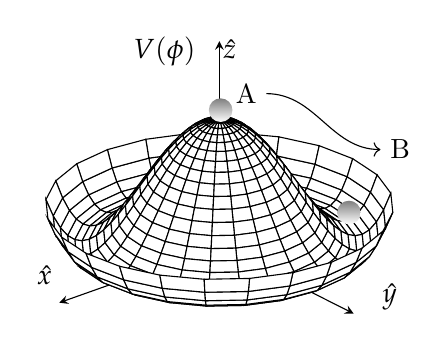
\begin{tikzpicture}
      \begin{axis}[
          axis lines=center,
          view={140}{25},
          axis equal,
          domain=0:360,
          y domain=0:1.25,
          xmax=1.5,ymax=1.5,zmin=0,zmax=1.5,
          x label style={at={(axis description cs:0.18,0.29)},anchor=north},
          y label style={at={(axis description cs:0.82,0.25)},anchor=north},
          z label style={at={(axis description cs:0.44,0.8)},anchor=north},
          xlabel = $\hat{x}$,
          ylabel=$\hat{y}$,
          zlabel=$V(\phi)\quad \hat{z}$,
          ticks=none,
          clip bounding box=upper bound
        ]
    
        \addplot3 [surf, shader=flat, draw=black, fill=white, z buffer=sort] ({sin(x)*y}, {cos(x)*y}, {(y^2-1)^2});
      \end{axis}
      \shade (3.47,3.5) circle [radius=0.15cm];
      \shade (5.1,2.2) circle [radius=0.15cm];
      \node[anchor=east] at (4.05,3.71) (text) {A};
      \node[anchor=west] at (5.5,3.0) (description) {B};
      \draw (description) edge[out=180,in=0,<-] (text);
    \end{tikzpicture}
    }
    \caption{Illustration of the Higgs potential. There is an infinite number of ground states. At point A, the global symmetry is unbroken. At point B, a local minimum is chosen and spontaneous symmetry breaking occurs. This figure is from Ref.~\cite{higgspotential}.}
    \label{fig:Higgspotential}
\end{figure}
\subsubsection{Broken continuous symmetry}

The previous section illustrates an example of spontaneous symmetry breaking. The original Lagrangian of equation \ref{eq:ssbLagrangian} is invariant if $phi\rightarrow-\phi$; it is even in $\phi$. In the reformed Lagrangian of equation \ref{eq:ssbReformedLagrangian}, however, this symmetry is broken because it is not even in $\eta$. The breaking is considered spontaneous because no external agent is required; the symmetry simply becomes hidden when selecting a particular ground state (the "vacuum"). In section \ref{sec:SSB} the broken symmetry was a discrete symmetry in context of a read scalar field. This section will apply spontaneous symmetry breaking to a complex scalar field.

Consider the following complex scalar field, written neatly as a combination of two real fields:
\begin{equation}
    \phi\equiv\dfrac{1}{\sqrt{2}}(\phi_1+i\phi_2)\\ \label{eq:complexfield}
    \phi^*\phi=\dfrac{1}{2}(\phi^2_1+\phi^2_2).
\end{equation}
The Lagrangian written with respect to the two fields $\phi_1$ and $\phi_2$ is
\begin{equation}\label{eq:SSBContLagrangian}
    \Lagrangian=\dfrac{1}{2}(\partial_{\mu}\phi_1)(\partial^{\mu}\phi_1) + \dfrac{1}{2}(\partial_{\mu}\phi_2)(\partial^{\mu}\phi_2) - \Big[\dfrac{1}{2}\mu^2(\phi_1^2+\phi_2^2)+\dfrac{1}{4}\lambda(\phi_1^2+\phi_2^2)^2\Big]
\end{equation}
where the terms in the square brackets is the potential energy function $V$. The minima of $V$ is a circle with the equation
\begin{equation}
    \phi_1^2+\phi_2^2=\dfrac{-\mu^2}{\lambda}=\nu^2
\end{equation}
where $\nu$ corresponds to the ground states. Arbritrarily one can choose
\begin{equation}
    \phi_1=\nu,\qquad\phi_2=0
\end{equation}
and introduce fluctuations about this vacuum state as new fields
\begin{align}\label{eq:etaxifields}
    \eta\equiv\phi_1-\nu,\qquad\xi\equiv\phi_2.
\end{align}

Now equation \ref{eq:SSBContLagrangian} can be rewritten in terms of $\eta$ and $\xi$:
\begin{equation}
    \Lagrangian=\Big[ \dfrac{1}{2}(\partial_{\mu}\eta)(\partial^{\mu}\eta) - \mu^2\eta^2 \Big] 
    + \Big[ \dfrac{1}{2}(\partial_{\mu}\xi)(\partial^{\mu}\xi) \Big] + \text{higher order terms.}
\end{equation}
The first term is the free Lagrangian for the field $\eta$, which includes a mass term, giving $m_{\eta}=\sqrt{2}\mu$. The second term describes field $\xi$, which unlike $\eta$, turns out to be massless. This is Goldstone's theorem - the appearance of a massless spin 0 Goldstone boson is the result of a spontaneous broken continuous global symmetry \cite{Griffiths:2008zz}. 

\subsection{The Higgs mechanism}

The Higgs mechanisms involves spontaneous symmetry breaking of the complex field in equation \ref{eq:complexfield} in a Lagrangian that is locally gauge invariant. Consider the Lagrangian in equation \ref{eq:SSBContLagrangian}: it is invariant under global \Ugroup{1} transformation $\phi\rightarrow e^{iq\theta}\phi$, however not invariant under local \Ugroup{1} gauge transformation $\phi\rightarrow e^{iq\theta(x)}\phi$. In order to impose local gauge invariance, the derivatives must be replaced with the appropriate covariant derivatives
\begin{equation}
    \partial_{\mu}\rightarrow\mathcal{D}_{\mu}=\partial_{\mu}+igA_{\mu}
\end{equation}
where a new gauge field $A_{\mu}$ is introduced and transforms as
\begin{equation}
    A_{\mu}\rightarrow A_{\mu}-\partial_{\mu}\theta(x).
\end{equation}
The locally invariant Lagrangian for the complex scalar field $\phi$ becomes
\begin{equation}\label{eq:Lagrcomplexscalarfield}
    \Lagrangian=(\covd_{\mu}\phi^*)(\covd^{\mu}\phi)-\mu^2\phi^2-\lambda\phi^4-\dfrac{1}{4}F_{\mu\nu}F^{\mu\nu}
\end{equation}
where the additional term is the Proca Lagrangian acccompanying the gauge field. 

As with the previous section, when $\mu^2<0$ in the potential, the choice of a physical degenate vacuum state breaks the symmetry of the Lagrangian. The complex scalar field can be rewritten by substituting equation \ref{eq:etaxifields} into equation \ref{eq:complexfield} to get:
\begin{equation}\label{eq:complexscalarfieldvev}
    \phi(x)=\dfrac{1}{\sqrt{2}}\Big[\nu+\eta(x)+i\xi(x)\Big].
\end{equation}
The definition above is used to rewrite the Lagrangian on equation \ref{eq:Lagrcomplexscalarfield} as
\begin{equation}
    \Lagrangian=\dfrac{1}{2}(\partial_{\mu}\eta)(\partial^{\mu}\eta) - \lambda\nu^2\eta^2
                + \dfrac{1}{2}(\partial_{\mu}\xi)(\partial^{\mu}\xi) 
                - \dfrac{1}{4}F_{\mu\nu}F^{\mu\nu} + \dfrac{1}{2}g^2\nu^2A_{\mu}A^{\mu}
                + g\nu A_{\mu}({\partial^{\mu}\xi})
                + \text{int. terms}
\end{equation}
where the first two terms represent the massive scalar field $\eta$, the third term corresponds to the massless Goldstone boson $\xi$, and the fourth and fifth terms describes the gauge field $A_{\mu}$ which has now acquired a mass. Additional three and four point interactions terms also exist the fields. The is the exact same Lagrangian as equation \ref{eq:Lagrcomplexscalarfield}; $\phi$ has simply been expanded about the vacuum state. The underlying symmetry of the \Ugroup{1} gauge group has consequently been broken.

The final step involves the choice of an appropriate gauge which eliminates the Goldstone field completely from the Lagrangian. This is motivated by the $q\nu A_{\mu}({\partial^{\mu}\xi})$ term, which reads as a coupling between the spin-1 gauge field $A_{\mu}$ and the spin-0 scalar Goldstone field $\xi$, where one field can transform into another. Such bilinear terms indicate that the fundamental fields have been misidentified \cite{Griffiths:2008zz}. The freedom in gauge choice is exploited to set 
\begin{equation}
    \theta(x)=-\dfrac{\xi(x)}{g\nu}
\end{equation}
which leads the complex scalar field to transform as 
\begin{equation}
    \phi(x)\rightarrow e^{-ig\frac{\xi(x)}{g\nu}}\phi(x).
\end{equation}
Writing equation \ref{eq:complexscalarfieldvev} to to first order as $\phi\approx\dfrac{1}{\sqrt{2}}\Big[\nu+\eta(x)\Big]e^{i\frac{\xi(x)}{\nu}}$, the gauge transformation on $\phi$ transforms away the Goldstone field completely:
\begin{equation}
    \phi(x)\rightarrow e^{-i\frac{\xi(x)}{\nu}} \dfrac{1}{\sqrt{2}}\Big[\nu+\eta(x)\Big]e^{i\frac{\xi(x)}{\nu}}
    = \dfrac{1}{\sqrt{2}}\Big[\nu+h(x)\Big].
\end{equation}
This choice of gauge renders $\phi$ to be entirely real, and is called the unitary gauge. Here the field $\eta(x)$ can be rewritten as $h(x)$, corresponding to none other than the Higgs field. The mass terms for the scalar Higgs field is 
\begin{equation}
    m_{\Higgs} = g\nu
\end{equation}
and the mass of $A$, the gauge boson associated with the local gauge symmetry, is given by
\begin{equation}
    m_A=\sqrt{2\lambda}\nu.
\end{equation}

\subsection{The Standard Model Higgs}

This final subsection will apply the Higgs mechanism to the electroweak sector of the Standard Model, with a \SUgroup{2}$_L\times$\Ugroup{1}$_Y$ local gauge symmetry. 
\begin{equation}
    \phi=
    \begin{pmatrix}
         \phi^+ \\
         \phi^0
    \end{pmatrix}
    =\dfrac{1}{\sqrt{2}}
    \begin{pmatrix}
         \phi_1+i\phi_2\\
         \phi_3+i\phi_4
    \end{pmatrix}
\end{equation}
\begin{equation} \label{eq:higgsLagr}
    \Lagrangian=(\covd_{\mu}\phi)(\covd^{\mu}\phi)^{\dagger}-V(\phi^{\dagger}\phi)
\end{equation}
\begin{equation}
    \dfrac{1}{2}(\phi_{1}^2+\phi_{2}^2+\phi_{3}^2+\phi_{4}^2)=\dfrac{\nu^2}{2}
\end{equation}
The Lagrangian has an infinite set of ground states, and choosing any particular ground state will break the symmetry. The vacuum state chosen is
\begin{equation}
    \bra{0}\phi\ket{0}=\dfrac{1}{\sqrt{2}}
    \begin{pmatrix}
         0 \\
         \nu
    \end{pmatrix}
\end{equation}
which keeps the ground state electrically neutral, and consequently the photon massless. Expanding the ground state as before, $\phi$ is redefined as 
\begin{equation}
    \phi(x) = e^{\frac{\xi_a(x)\sigma_a}{2\nu}}\dfrac{1}{\sqrt{2}}
    \begin{pmatrix}
         0\\
         \nu+h(x)
    \end{pmatrix}.
\end{equation}
Choosing a unitary gauge, the Higgs double is rewritten such that the massless Goldstone fields are "eaten" by the gauge fields and the dependence on $\xi_a$ is removed.
\begin{equation} \label{eq:higgsvev}
    \phi(x)\rightarrow e^{-\frac{\xi^a(x)\sigma^a}{2\nu}}\phi(x)=\dfrac{1}{\sqrt{2}}
    \begin{pmatrix}
         0\\
         \nu+h(x)
    \end{pmatrix}.
\end{equation}
Applying equation \ref{eq:higgsvev} on the kinematic part of the Lagrangian in equation \ref{eq:higgsLagr} and expanding generates the mass terms of the gauge boson fields. In the unitary gauge, $\covd_{\mu}\phi$ is
\begin{align}
    \mathcal{D}_{\mu}\phi & = \Big[\partial_{\mu}+ig_W\dfrac{\sigma^a}{2}W^a_{\mu}+ig'\dfrac{Y}{2}B_{\mu}\Big]\phi\\
        & = \dfrac{1}{\sqrt{2}}
        \begin{pmatrix}
             \partial_{\mu} + \dfrac{ig_W}{2}W_{\mu}^3 + \dfrac{ig'}{2}B_{\mu} & \dfrac{ig_W}{2}(W_{\mu}^1-iW_{\mu}^2) \\
             \dfrac{ig_W}{2}(W_{\mu}^1+iW_{\mu}^2) & \partial_{\mu} - \dfrac{ig_W}{2}W_{\mu}^3 + \dfrac{ig'}{2}B_{\mu}
        \end{pmatrix}
        \begin{pmatrix}
             0 \\
             \nu+h
        \end{pmatrix}\\
        & = \dfrac{1}{\sqrt{2}}
        \begin{pmatrix}
             \dfrac{ig_W}{2}(W_{\mu}^1-iW_{\mu}^2)(\nu+h)\\
             (\partial_{\mu}-\dfrac{ig_W}{2}W_{\mu}^3+\dfrac{ig'}{2}B_{\mu})(\nu+h).
        \end{pmatrix}
\end{align}
The kinetic term $(\covd_{\mu}\phi)(\covd^{\mu}\phi)^{\dagger}$ is
\begin{align}
    (\covd_{\mu}\phi)(\covd^{\mu}\phi)^{\dagger} = &  \dfrac{1}{2}(\partial_{\mu}h)(\partial^{\mu}h) + \dfrac{1}{8}g_ W^2(W_{\mu}^1+iW_{\mu}^2)(W^{1\mu}-iW^{2\mu})(\nu+h)^2\\
    & + \dfrac{1}{8}(g_W W_{\mu}^3 - g'B_{\mu})(g_W W^{3\mu} - g'B^{\mu})(\nu+h)^2
\end{align}

\begin{align}
    m_W & =\dfrac{1}{2}g_{W}\nu\\
    m_Z & =\dfrac{1}{2}\nu\sqrt{g_W^2+g'^2}\\
    m_A & =0.
\end{align}
The spontaneous breaking of the \Ugroup{1}$_Y\times$\SUgroup{2}$_{L}$ symmetry lets the $W$ and $Z$ bosons acquire mass, while the \Ugroup{1}$_Q$ symmetry remains unbroken thus leaving the photon massless. 

\subsection{Yukawa sector: fermion masses}

The fermionic mass term given by 
\begin{equation}
    -m\bar{\psi}\psi=-m(\overline{\psi}_R\psi_L+\psi_R\overline{\psi}_L)
\end{equation}
is not invariant under a local gauge transformation due to different transformation properties of its left- and right-handed chiral components. The left-handed states transform as weak isospin doublets under \SUgroup{2}$_L$, while the right-handed states transform as singlets. 

It is possible to add interaction terms between the Higgs field and the fermions to the Lagrangian of equation \ref{eq:higgsLagr} while preserving the \SUgroup{2}$_L\times$\Ugroup{1}$_Y$ symmetry. Starting with leptons, this is done by writing the term
\begin{equation}
    \Lagrangian_{\text{Yukawa, }\ell}=-c_{\ell} (\overline{\psi}_R\phi^{\dagger}\psi_L+\psi_R\phi\overline{\psi}_L)
\end{equation}
where $c_{\ell}$ is the Yukawa coupling constant between the specified lepton and the Higgs field. Next, the Higgs doublet $\phi$ is replaced with the ground state written in unitary gauge as per equation \ref{eq:higgsvev}, and the Lagrangian becomes
\begin{align}
    \Lagrangian_{\text{Yukawa, }\ell} & = -\dfrac{c_{\ell}}{\sqrt{2}}\nu(\overline{\psi}_R\psi_L+\psi_R\overline{\psi}_L) - \dfrac{c_{\ell}}{\sqrt{2}}h(\overline{\psi}_R\psi_L+\psi_R\overline{\psi}_L)\\
             & = -\dfrac{c_{\ell}}{\sqrt{2}}\nu\overline{\psi}\psi - \dfrac{c_{\ell}}{\sqrt{2}}\overline{\psi}\psi h \\
             & = -m_{\ell}\overline{\psi}\psi - \dfrac{m_{\ell}}{\nu}\overline{\psi}\psi h.
\end{align}
The first term is a mass term for the lepton, and the second term represents the coupling of the lepton to the Higgs boson. 

The same mechanism generates mass for the case of down-type quarks. Up-type quarks require something a little different. The vacuum expectation value for the Higgs doublet is zero in the upper component, and therefore cannot generate mass for the up-type quarks and neutrinos\footnote{The question of neutrino masses will not be address in this thesis.}. Focusing on the case of the up-type quarks $\psi_u$, it is useful to define the conjugate doublet $\phi_C$
\begin{equation}
    \phi_C = -i\sigma_2\phi^* = 
    \begin{pmatrix}
         -\phi^{0*} \\
         \phi^-
    \end{pmatrix}
    = \dfrac{1}{\sqrt{2}}
    \begin{pmatrix}
         -\phi_3+i\phi_4\\
         \phi_1-i\phi_2
    \end{pmatrix}.
\end{equation}
which transforms exactly like $\phi$. Now a gauge invariant Yukawa term can be written for the quark families as
\begin{equation}
    \Lagrangian_{\text{Yukawa, }q}=-c_u (\overline{\psi}_{u,R}\phi_C^{\dagger}\psi_{u,L}+\psi_{u,R}\phi_C\overline{\psi}_{u,L}) - c_d (\overline{\psi}_{d,R}\phi^{\dagger}\psi_{d,L}+\psi_{d,R}\phi\overline{\psi}_{d,L})
\end{equation}
which becomes
\begin{align}
    \Lagrangian_{\text{Yukawa, }q} & = - \dfrac{c_u}{\sqrt{2}}\nu\overline{\psi}_u\psi_u - \dfrac{c_u}{\sqrt{2}}\overline{\psi}_u\psi_uh - \dfrac{c_d}{\sqrt{2}}\nu\overline{\psi}_d\psi_d - \dfrac{c_d}{\sqrt{2}}\overline{\psi}_d\psi_dh \\
                & = -m_u\overline{\psi}_u\psi_u - \dfrac{m_u}{\nu}\overline{\psi}_u\psi_u h - m_d\overline{\psi}_d\psi_d - \dfrac{m_d}{\nu}\overline{\psi}_d\psi_d h
\end{align}
after spontaneous symmetry breaking.
The Yukawa constants $c_q, c_{\ell}$ are not predicted by theory, and are assigned values that are consistent with experimental fermion mass measurements. 
%   \chapter{The Large Hadron Collider and the ATLAS experiment}
\label{chap:ATLASdetector}
%% LHC and ATLAS introduction
\section{The Large Hadron Collider}
\label{sec:LHC}

This massive fruit of labour, decades in the making from the hundreds of institutions which make up CERN, lies hidden 100 meters below the surface of the Switzerland-France border. Sandwiched between Geneva and the Jura Mountains is a 27 km ring of superconducting magnets and radio-frequency (RF) cavities, which bend and accelerate particles to near light speed. More specifically, it is approximately 3 metres per second slower. This remarkable achievement is none other than the Large Hadron Collider (LHC). The LHC lives up to its name; it is the largest machine built by humankind, and unsurprisingly the most powerful high-energy particle collider in the world. The four main interaction points around the ring where particles collide mark the four main experiments: ATLAS, CMS, LHCb, and ALICE~\cite{LHCMachine}. The former two are general purpose detectors with a similar goal: to precisely study the Standard Model and to search for evidence of new physics. The latter two have specialized purposes. LHCb is dedicated to probing physics involving b-hadrons in pp collisions, and ALICE’s aim is to shed light on the physics of the quark-gluon plasma by investigating heavy-ion collisions. 

The protons used in the collisions originally come from hydrogen gas. The gas is housed in tanks and stripped of orbital electrons through
of ionization. Prior to the injection into the LHC, the protons first pass through a series of smaller machines which boost them to higher and higher energy. The first in the chain is LINAC2, a linear accelerator in which beams of protons are formed, and given an energy of \unit{50}{\MeV}. Next the protons are piped into the Proton Synchrotron Booster, the Proton Synchrotron, and finally into the Super Proton Synchrotron \todo{Give more details about each of these steps}. Through this chain the protons get boosted to \unit{1.4}{\GeV} by the PSB, then further to \unit{25}{\GeV} by the PS, to a final \unit{450}{\GeV} by the SPS before entering the LHC. Inside the pipes of the LHC, the protons take a short 20 minutes to reach \unit{6.5}{\TeV}. 

\begin{figure}
  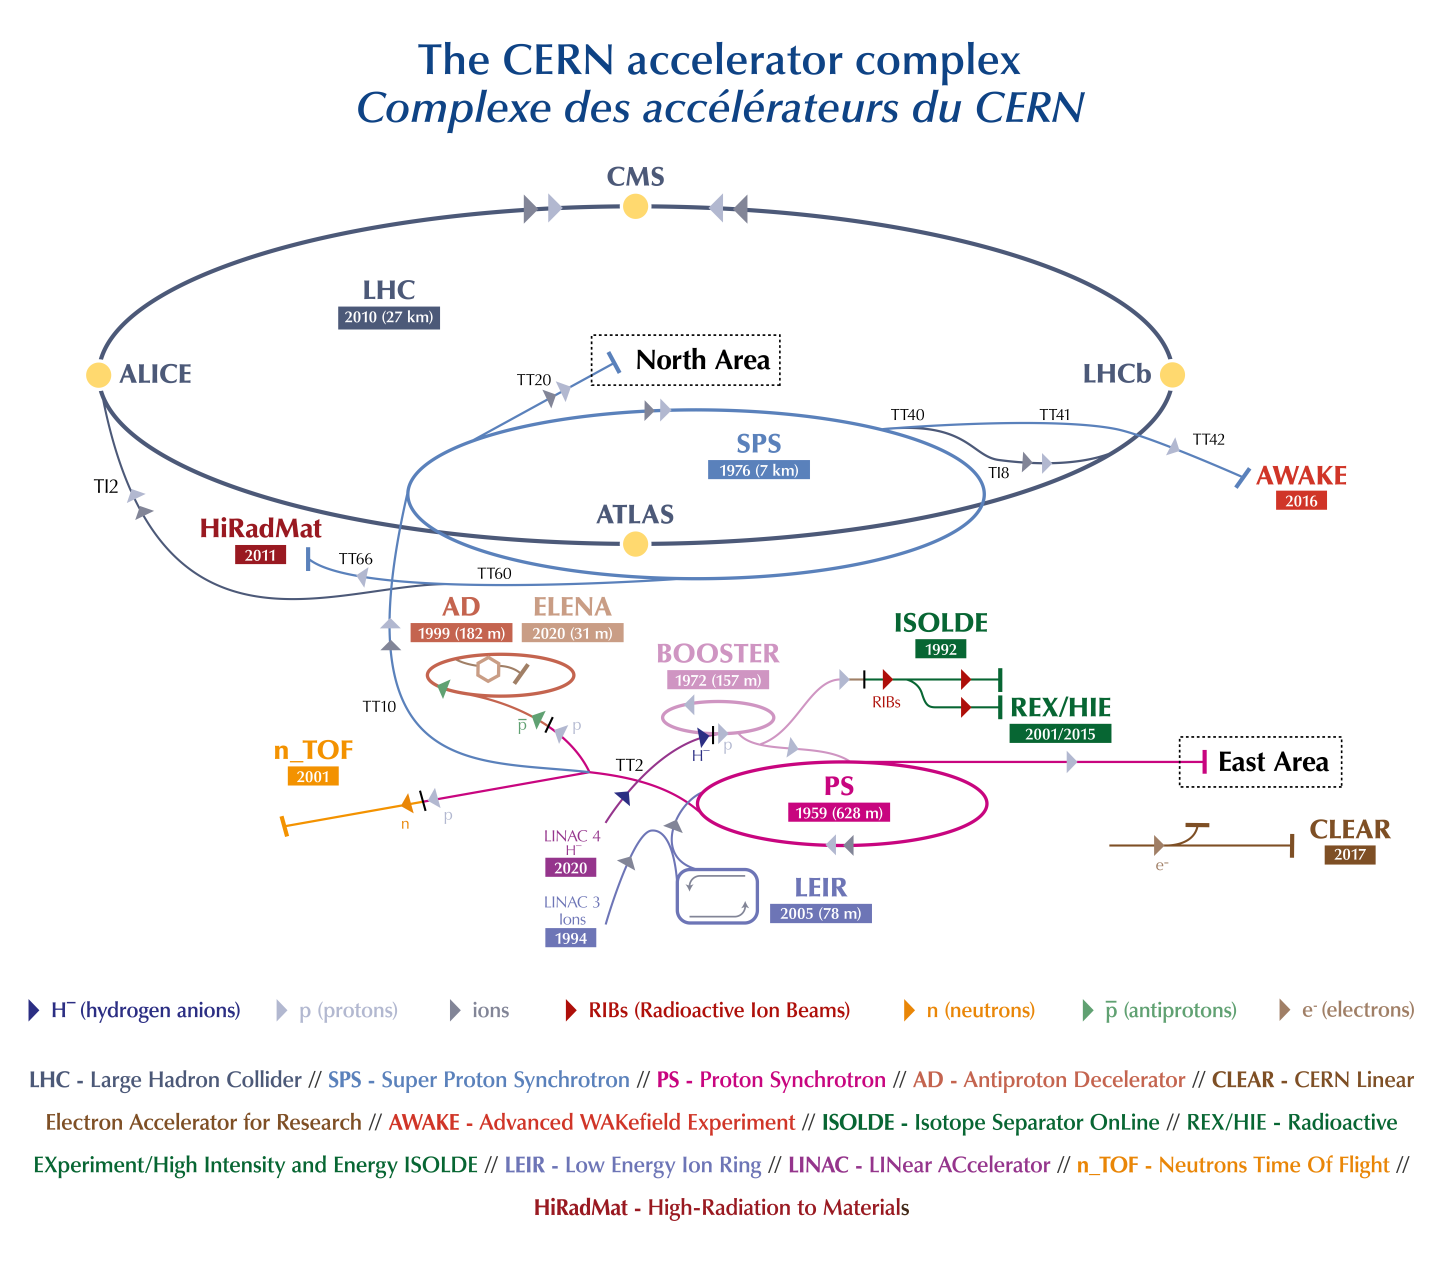
\includegraphics[width=0.9\textwidth]{Figures/LHC/CernAcceleratorComplex.png}
  \caption[The \CERN accelerator complex]%
  {The CERN accelerator complex, where the LHC is the largest ring. The four main collision points corresponding to the main experiments are dotted in yellow. This figure is from Ref.~\cite{Mobs:2684277}.}
  \label{fig:CERNComplex}
\end{figure}

The impressive feat of accelerating particles is made possible through the use of radio-frequency cavities. The idea was first crafted by the young Rolf Wideröe \cite{vretenar2012radio} for his PhD thesis and later caught the eye of the brilliant E. Lawrence, recipient of the Nobel Prize in Physics in 1939 for the invention of the cyclotron. RF cavities are round chambers along the beam. A voltage generator generate a voltage which oscillates at \unit{400}{\mega\hertz}, inducing an electric field inside the RF cavity. As particles pass through they experience the force of the field and are accelerated along the beam pipe. In total the LHC uses 8 RF cavities per beam (so 16 in total), with each cavity capable of delivering two megavolts of energy. Protons travelling through the cavity increase their energy to 14 times the injection amount, from 450 GeV to 6.5 TeV. Once protons get up to speed, a proton that has perfect timing are left alone, while protons that arrive slightly earlier/later will be accelerated/decelerate. The result is a beam of protons sorted into smaller segments of proton bunches. The LHC produces two such proton beams, one circulating clockwise and the other counterclockwise. 

A key concept in particle physics is luminosity. It is a factor that relates the cross-section to the number of event per second, written as follows:
\begin{equation}
    \luminosity=\dfrac{1}{\sigma}\cdot\dfrac{dN}{dt}
\end{equation}
where \luminosity is the luminosity, $N$ is the number of events, and $\sigma$ is the production cross section. The dimension of luminosity is events per unit time and unit area \unit{}{\cm\rpsquared}\unit{}{\second\rp}.

There are two properties used to describe a particle beam: its \todo{write more about this} emittance $\epsilon$, and its $\beta$ function. The emittance can be thought of as the area occupied by the particle beam in the position momentum plane. A lower emittance means the distance between particles and the difference in momentum between the particles are small. The $\beta$ function is also known as the amplitude function. It is a function related to the transverse size of the particle beam, and it is proportional to the width of the beam squared divided by the emittance. With low $\beta$, the beam is narrowere and squeezed. When high $\beta$, the beam is wider. The cross sectional sizes of the beam $\sigma_i$ ($i=x,y$) are written as 
\begin{equation}
    \sigma_i=\sqrt{\dfrac{\beta_i\cdot\epsilon_i}{\pi}}
\end{equation}
The beams are assumed to be Gaussian distributed, meaning that in collisions, the centres of the beams contribute most while the edges have minimal impact. Following this the luminosity is
\begin{equation}
    \luminosity=\dfrac{N_1N_2f_{rev}N_b}{2\pi\Sigma_x\Sigma_y}
\end{equation}
where $N_1$ and $N_2$ are the number of particles for each bunch, $N_b$ is the number of bunches, $f$ is the revolution frequency, and $\Sigma_x,\Sigma_y$ represent the \unsure[]{Read more about this!} convolution of the beam sizes. They can be expressed as
\begin{equation}
    \Sigma_x=\sqrt{\sigma_{x1}^2+\sigma_{x2}^2}, \quad \Sigma_y=\sqrt{\sigma_{y1}^2+\sigma_{y2}^2}.
\end{equation}
Assuming that the beam sizes are identical and round, $\sigma_{x1}=\sigma_{x2}=\sigma_{y1}=\sigma_{y2}$, and the luminosity becomes
\begin{equation}
    \luminosity=\dfrac{N_1N_2f_{rev}N_b}{4\pi\sigma^2}=\dfrac{N_1N_2f_{rev}N_b\gamma}{4\pi\epsilon_N\beta^*},
\end{equation}
where $\beta^*$ is the amplitude function at the interaction point. The LUCID-2 detector of the LHC consists of several small Cherenkov detectors that consists only of photomultipliers with quartz windows, and it is responsible for luminosity measurements and luminosity monitoring~\cite{Avoni:2633501}. 

When proton beams cross at the LHC, there are many collisions which occur other than the hard-scatter of interest. While increasing the number of particles per bunch increases the likelihood of a rare interaction, it also increases the pile-up of multiple interactions. The number of pile-up events, denoted as $\mu$, is one of the biggest obstacles for LHC experiments; the more there is, the more difficult it becomes to disentangle the events of interest from the sea of low energy collisions. It is, however, an inevitable consequence that accompanies increasing the instantaneous luminosity. The contribution to pile-up events can be separated into two main categories: 
\begin{itemize}
  \item In-time pile-up refers to simultaneous proton-proton collisions occurring in the same bunch crossing as the hard scatter of interest;
  \item Out-of-time pile-up is the overlay of events from neighbouring bunches which contaminate signal events, attributed to detector electronics latency.
\end{itemize}
There are also less-substantial contributions from the cavern background, beam halo events, and beam gas events. The cavern background is the cloud of gas that floods the LHC cavern during operation. Beam halo events are from when the proton beam interacts with the collimating instrumentation, and the beam gas events describe interactions between the beam and the residual gas in the beam pipe. 

The \LHC was originally designed to reach a peak instantaneous luminosity and average pile-up of \unit{$10^{34}$}{\rpsquare{\cm}\reciprocal{\second}}\todo{Citation?} and $\langle\mu\rangle=19$ respectively. In Run II, the LHC reached peak luminosity of $2\times$\unit{$10^{34}$}{\rpsquare{\cm}\reciprocal{\second}}, and peak pile-up of $\mu=60$~\cite{boyd2020lhc}. Figure \ref{fig:Pileup} shows the profiles of pile-up conditions in the four years of operation. 

\begin{figure}
  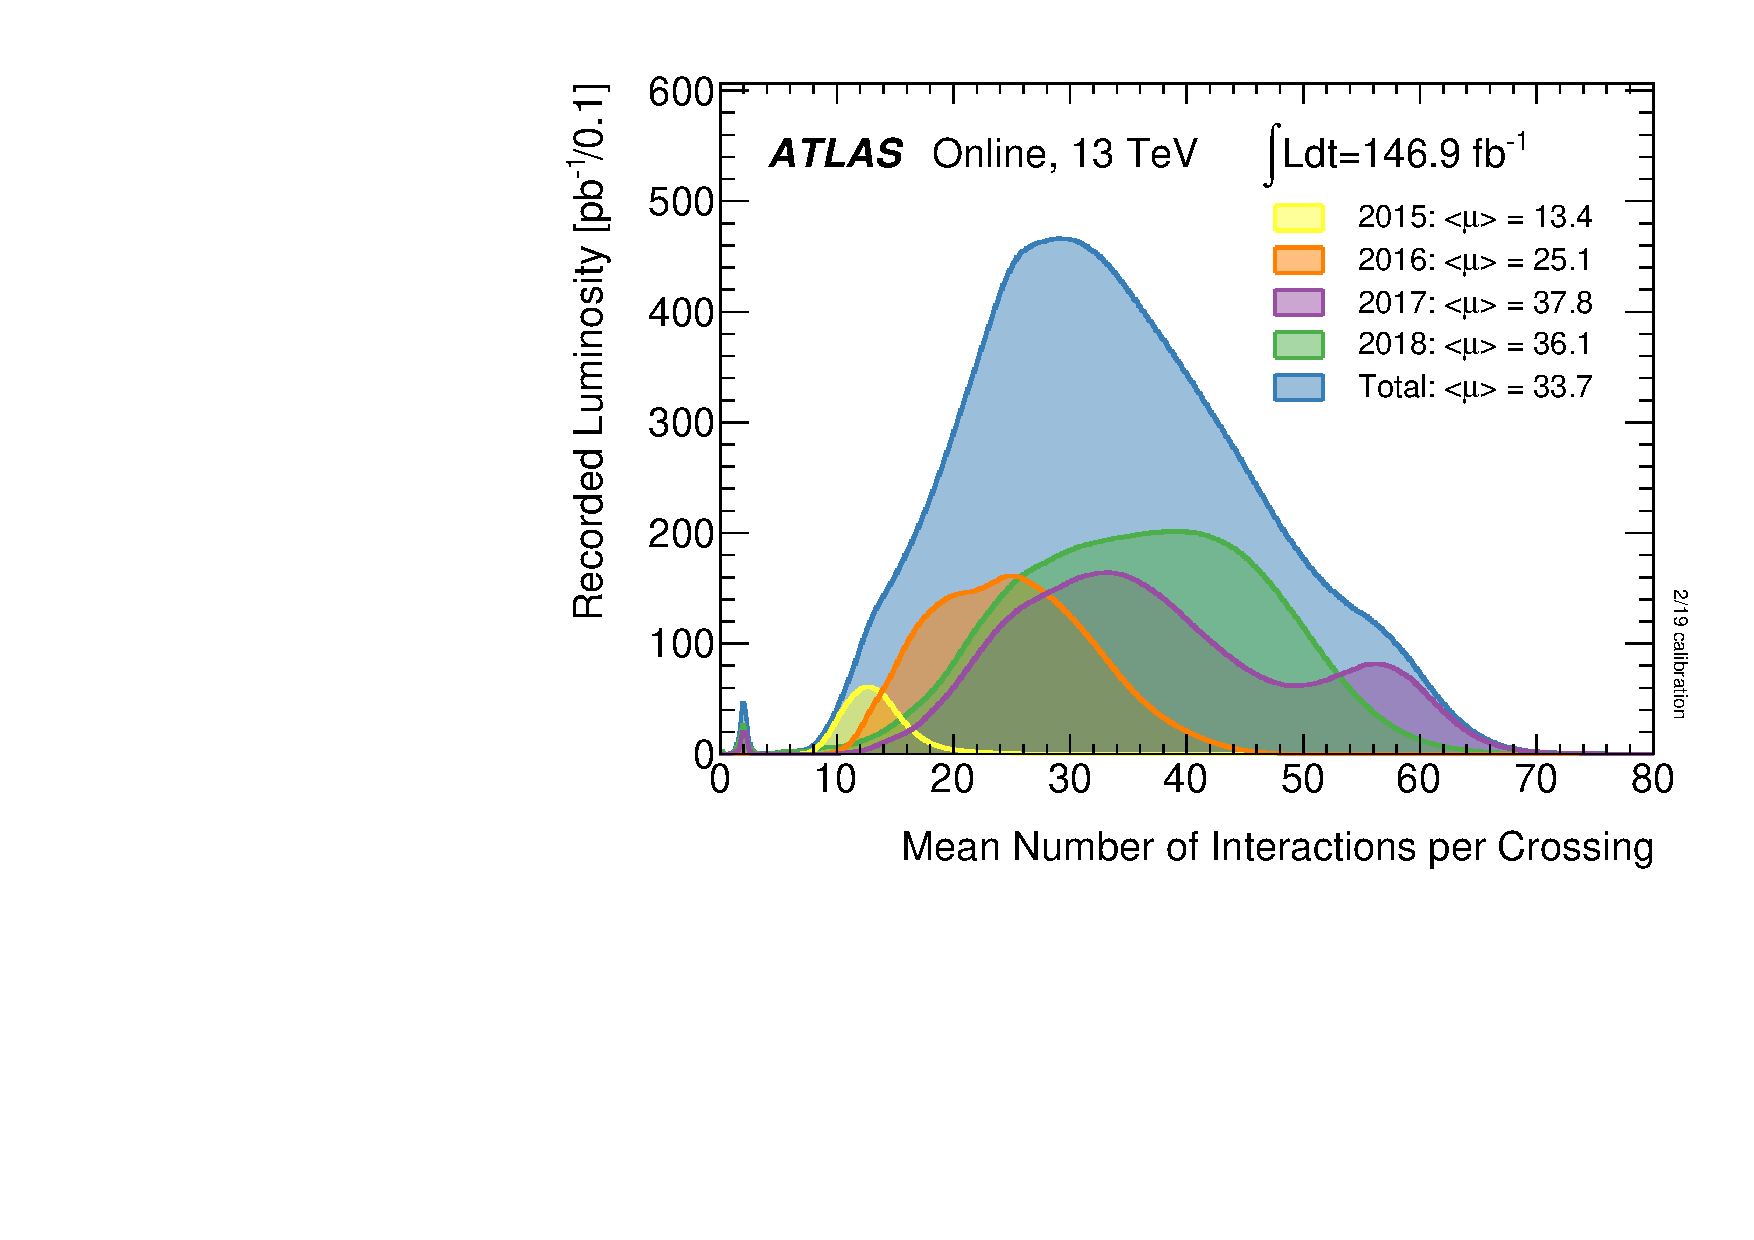
\includegraphics[width=0.7\textwidth]{Figures/LHC/PileUp_2015_2018.pdf}
  \caption[Pile-up distributions.]
  {The pile-up, $\mu$, is the mean number of collisions per bunch crossing. Shown are the pile-up distributions from 2015-2018, where each distribution is luminosity weighted. This figure is from Ref.~\cite{pileupatlas}.}
  \label{fig:Pileup}
\end{figure}

\section{The ATLAS detector}\label{sec:ATLAS}

Measuring forty-six meters in length, twenty five meters in height and width, and weighing in at a hulking seven thousand tons, the ATLAS (A-Toroidal-LHC-ApparatuS) detector is the Mount Everest of particle detectors. Built with a cylindrical and symmetric structure around the beam pipe, it's detection region covers nearly the entirety of the $4\pi$ solid angle of the collision point. \ATLAS is a general purpose detector, and combines a multitude of detector technologies to conduct searches for new phenomena, and to make high-precision measurements of the Standard Model.

The right-handed coordinate system used by the ATLAS detector, and also very commonly in particle physics, is illustrated in figure \ref{fig:atlascoordinate}. The $z$-axis is parallel to the beam pipe, the $y$-axis points vertically to the sky, and the $x$-axis points to the centre of the \LHC ring. The $xy$-plane is often referred to as the transverse plane, and the frequently encountered variables $p_T$ and $E_T$ refer to the momentum and energy in the transverse direction respectively. The azimuthal angle in the transverse plane is denoted as $\phi$, and polar angle $\theta$ denotes the angle offset from the beam pipe. Another commonly used coordinate is the rapidity, $y$, of an object:
\begin{equation}
    y=\dfrac{1}{2}\ln\dfrac{E+p_Z}{E-p_Z},
\end{equation}
where $E$ is the object's energy and $p_Z$ is the momentum in the $z$-direction. Rapidity differences are invariant
with respect to Lorentz boosts along the beam axis. This is the key reason why rapidities are so crucial in accelerator physics~\cite{daw2012}. Alternatively there is the pseudorapidity $\eta$ in the massless limit:
\begin{equation}
    \eta=-\ln\tan \dfrac{\theta}{2}.
\end{equation}
Both rapidity and pseudorapidity are more commonly used than polar angle $\theta$. The separation of two detected objects, $\Delta R$, is given by
\begin{equation}
    \Delta R=\sqrt{\Delta y^2+\Delta\phi^2},
\end{equation}
which is Lorentz invariant under a boost along the longitudinal (beam) direction.

The rest of this section will review the three sub-detectors of \ATLAS - the Inner Detector, the Calorimeter, and the Muon Spectrometer - as well as the Magnet System. A cross-sectional diagram illustrating the sub-detector systems is shown in Figure \ref{fig:atlasdetector}. The sub-detectors are made up of concentric barrels that wrap around the beam pipe, and circular endcaps placed at either end of the barrels. The barrels are designed to detect the particles that travel through the central $|\eta|$ region, and the endcaps broadens the angular coverage for particles whose trajectories run close to parallel to the beam. 

\begin{figure}
    \centering
    \resizebox{.6\textwidth}{!}{
    \tdplotsetmaincoords{75}{50} % to reset previous setting
    \begin{tikzpicture}[scale=2.7,tdplot_main_coords,rotate around x=90]
 
     % variables
      \def\rvec{1.2}
      \def\thetavec{40}
      \def\phivec{70}
      \def\R{1.1}
      \def\w{0.3}
     
      % axes
      \coordinate (O) at (0,0,0);
      \draw[thick,->] (0,0,0) -- (1,0,0) node[below left]{$x$};
      \draw[thick,->] (0,0,0) -- (0,1,0) node[below right]{$y$};
      \draw[thick,->] (0,0,0) -- (0,0,1) node[below right]{$z$};
      \tdplotsetcoord{P}{\rvec}{\thetavec}{\phivec}
     
      % vectors
      \draw[->,red] (O) -- (P) node[above left] {$P$};
      \draw[dashed,red] (O)  -- (Pxy);
      \draw[dashed,red] (P)  -- (Pxy);
      \draw[dashed,red] (Py) -- (Pxy);
     
      % circle - LHC
      \tdplotdrawarc[thick,rotate around x=90,black!70!blue]{(\R,0,0)}{\R}{0}{360}{}{}
     
      % compass - the line between CMS and ATLAS has a ~12° declination (http://googlecompass.com)
      \begin{scope}[shift={(1.1*\R,0,1.65*\R)},rotate around y=12]
        \draw[<->,black!50] (-\w,0,0) -- (\w,0,0);
        \draw[<->,black!50] (0,0,-\w) -- (0,0,\w);
        \node[above left,black!50,scale=0.6] at (-\w,0,0) {N};
      \end{scope}
     
      % nodes
      \node[left,align=center] at (0,0,1.1) {Jura};
      \node[right] at (\R,0,0) {LHC};
      \fill[radius=0.8pt,black!20!red]
        (O) circle node[left=4pt,below=2pt] {CMS};
      \draw[thick] (0.02,0,0) -- (0.5,0,0); % partially overdraw x-axis and CMS point
      \fill[radius=0.8pt,black!20!blue]
        (2*\R,0,0) circle
        node[right=4pt,below=2pt,scale=0.9] {ATLAS};
      \fill[radius=0.8pt,black!10!orange]
        ({\R*sqrt(2)/2+\R},0,{ \R*sqrt(2)/2}) circle % 45 degrees from ATLAS
        node[left=2pt,below=2pt,scale=0.8] {ALICE};
      \fill[radius=0.8pt,black!60!green]
        ({\R*sqrt(2)/2+\R},0,{-\R*sqrt(2)/2}) circle % 45 degrees from ATLAS
        node[below=2pt,right=2pt,scale=0.8] {LHCb};
     
      % arcs
      \tdplotdrawarc[->]{(O)}{0.2}{0}{\phivec}
        {above=2pt,right=-1pt,anchor=mid west}{$\phi$}
      \tdplotdrawarc[->,rotate around z=\phivec-90,rotate around y=-90]{(0,0,0)}{0.5}{0}{\thetavec}
        {anchor=mid east}{$\theta$}
 
    \end{tikzpicture}
    }
    \caption{The coordinate system used at the LHC in the perspective of the CMS experiment. Figure taken from~\cite{coordinatesys}.}
    \label{fig:atlascoordinate}
\end{figure}

\begin{figure}[htb!]
    \centering
    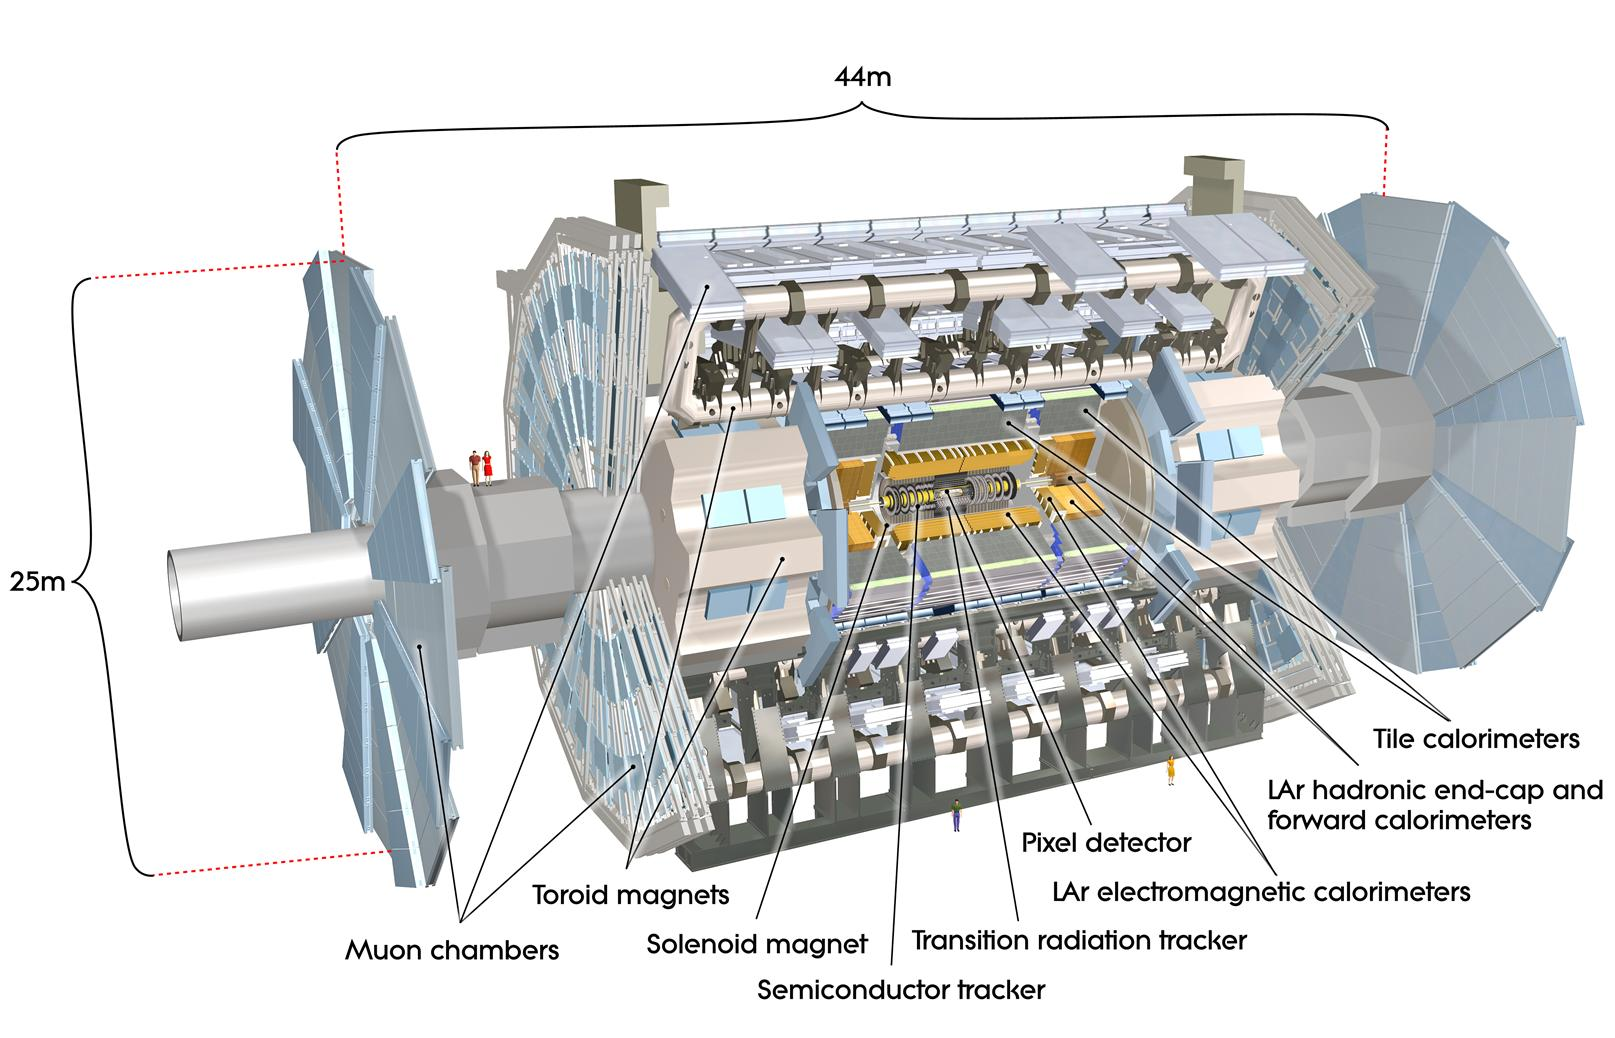
\includegraphics[width=0.7\textwidth]{Figures/LHC/ATLASDetector.jpg}
    \caption{The \ATLAS detector and its sub-components. This figure is from Ref.~\cite{Reed:2014}.}
    \label{fig:atlasdetector}
\end{figure}

\subsection{The Inner Detectors} \label{ssec:ATLASID}
The Inner Detector (ID) is able to measure the momentum of charged particles passing through it. The trajectories of the charged particles as they cross through are curved by a superconducting solenoid magnet with a 2 Tesla magnetic field~\cite{Yamamoto:1999}. The direction of curvature indicates the particle's charge, while the degree of curvature indicates momentum. The Inner Detector is the smallest sub-detector of ATLAS, stretching out to a radius of only 1.15 meters, with a total length of 7 meters. The barrel arrangement consists of concentric cylinders wrapped around the beam axis, and the end-cap components are attached as disks normal to the beam axis. The inner detector has three main components: the Pixel Detector, the Semiconductor Tracker (SCT), and the Transition Radiation Tracker (TRT).

\subsubsection{Pixel Detector}

The Pixel Detector is the innermost part of the Inner Detector. It is the part of ATLAS that is closest to the interaction point where particles collide. It was designed with extremely high granularity in mind in order to accurately resolve primary and secondary vertices, determine impact parameter resolution, and identify short-lived particles such as b-hadrons and tau leptons. Prior to Run 2, the pixel detector consisted of three concentric layers in the barrel, and three disks in the end-cap regions. During the long shutdown prior to Run 2, an additional layer called the Insertable B-layer (IBL)~\cite{Capeans:1291633} was added to the Pixel Detector closest to the beam pipe, making a total of four layers. The pixel detector are made up of sensor modules, each consisting of 46,080 active silicon pixels measuring 50 micrometers in width ($\phi$ direction) and 400 micrometers in length ($z$ direction). Each module consist of the active sensor medium (in this case silicon), and front-end electronics for readout. In total, the pixel detector hosts an astonishing eighty million readout channels. All together, the pixel detector achieves a resolution of \unit{10}{\micro\meter} in the $\phi$-direction and \unit{115}{\micro\meter} in the $z$-direction.

\subsubsection{Semi-conductor tracker}

The second layer of the inner detector is the SemiConductor Tracker (SCT), made up of two-sided modules of silicon microstrip sensors arranged back to back and tilted by a stereo angle of 40 mrad \cite{AHMAD200798}. It wraps around around the pixel detector and has in total 4088 modules, assembled in four cylindrical layers in the barrel region, and two end-caps containing nine disks each \cite{CERN-LHCC-2017-005}. The stereo angle enables the module to provide information about where along the strip the hit occurred. This is turn gives resolution in the z-plane in the barrels, and in R along the endcaps. The spatial resolution of the detector is \unit{17}{\mu\meter} in $R-\phi$ coordinate and \unit{580}{\mu\meter} in the $z$ coordinate in the barrel ($R$ in the endcaps) \cite{Abdesselam:974073}. In total the SCT hosts 4088 modules, assembled in four cylindrical layers in the barrel region, and two end-caps containing nine disks each \cite{CERN-LHCC-2017-005}. 

\subsubsection{Transition Radiation Tracker}

The third and outermost layer of the inner detector is the Transition Radiation Tracker (TRT). Unlike the ID and the SCT, it uses a straw drift tube technology, and exploits transition radiation emission for additional particle identification. Each module consists of 4 millimetre diameter straw tubes filled with xenon, carbon dioxide, and oxygen (70\%, 27\%, and 3\%)\cite{Vogel:1537991} bundled together. In order to collect charge from ionisation, a tungsten wire extends axially through the centre of each tube. In the barrel the drift tubes run parallel with the beam axis, and in the endcaps they run radially. In total there are 351,000 readout channels, and the resulting position resolution is weaker than the Pixel Detector or the SCT. The TRT is only capable of performing measurements in the $R-\phi$ coordinate, with a resolution of \unit{130}{\mu\meter}~\cite{Vogel:1537991}. 

Despite the lower resolution and the lack of sensitivity in the $z$ coordinate, the hits in the TRT contribute significantly to momentum resolution due to the a larger number of measurements and an extended measured track length. There are 73 parallel planes of straw-tubes in the barrel and 80 planes in each endcap. Furthermore, the barrel straws are inter-weaved in a matrix of polypropylene fibres, and the endcap disks are wedged in between polypropylene foils, creating numerous material boundaries. As highly relativistic particles pass through the boundaries they emit transition radiation photons; predominantly in the X-ray energy regime \cite{Ginzburg_1996}. These photons are absorbed by the gas mixture inside the tubes, and yield higher signal amplitudes than the signal of hits from minimum-ionizing particles. The energy of the transition radiation photon is strictly proportional to the relativistic factor $\gamma=E/m$ of the incident particle. For a given momentum, it is much higher for electrons than it is for pions or muons, a useful difference that is exploited for particle identification.

\subsection{Calorimetry}
Immediately after the particles exit the inner detector, they reach a set of calorimeters whose aim is to measure the particles’ energies by fully absorbing them. In contrast to the Inner Detector, the calorimeters can detect both charged and neutral particles. Neutrinos and muons, however, pass through the calorimeters unaffected as they are minimally ionizing particles (MIPs) at the LHC energy scale. The ATLAS calorimeters use sampling calorimeter technology. This is a design choice where layers of an active sensing material alternate with layers of a dense absorber material. Particles crossing the calorimeters will interact with the absorber medium and lose its energy through interactions. The initial traversing particle eventually creates a cascade of many lower energy particles - a particle shower. The sensitive detector medium sandwiched between will generate a signal proportional to this shower, with readout done through ionization or scintillation. 
There are two types of particle showers: electromagnetic and hadronic, depending on the nature of the source. Electromagnetic showers are primarily initiated by electrons or photons and develop mainly through Bremsstrahlung ($e\rightarrow\gamma e$) and pair production ($\gamma\rightarrow e^+e^-$), while hadronic interactions are more complex, developing through the strong interaction between the hadrons and the absorber material's nuclei. They differ radically, and thus require separate detector technologies for high-precision detection.  In order to meet these needs, there are two types of calorimeters that are hermetic along the $\phi$ coordinate and cover up to $|\eta| < 4.9$. As depicted in Figure \ref{fig:calorimeters}, these are the electromagnetic and the hadronic calorimeters. 

\begin{figure}
    \centering
    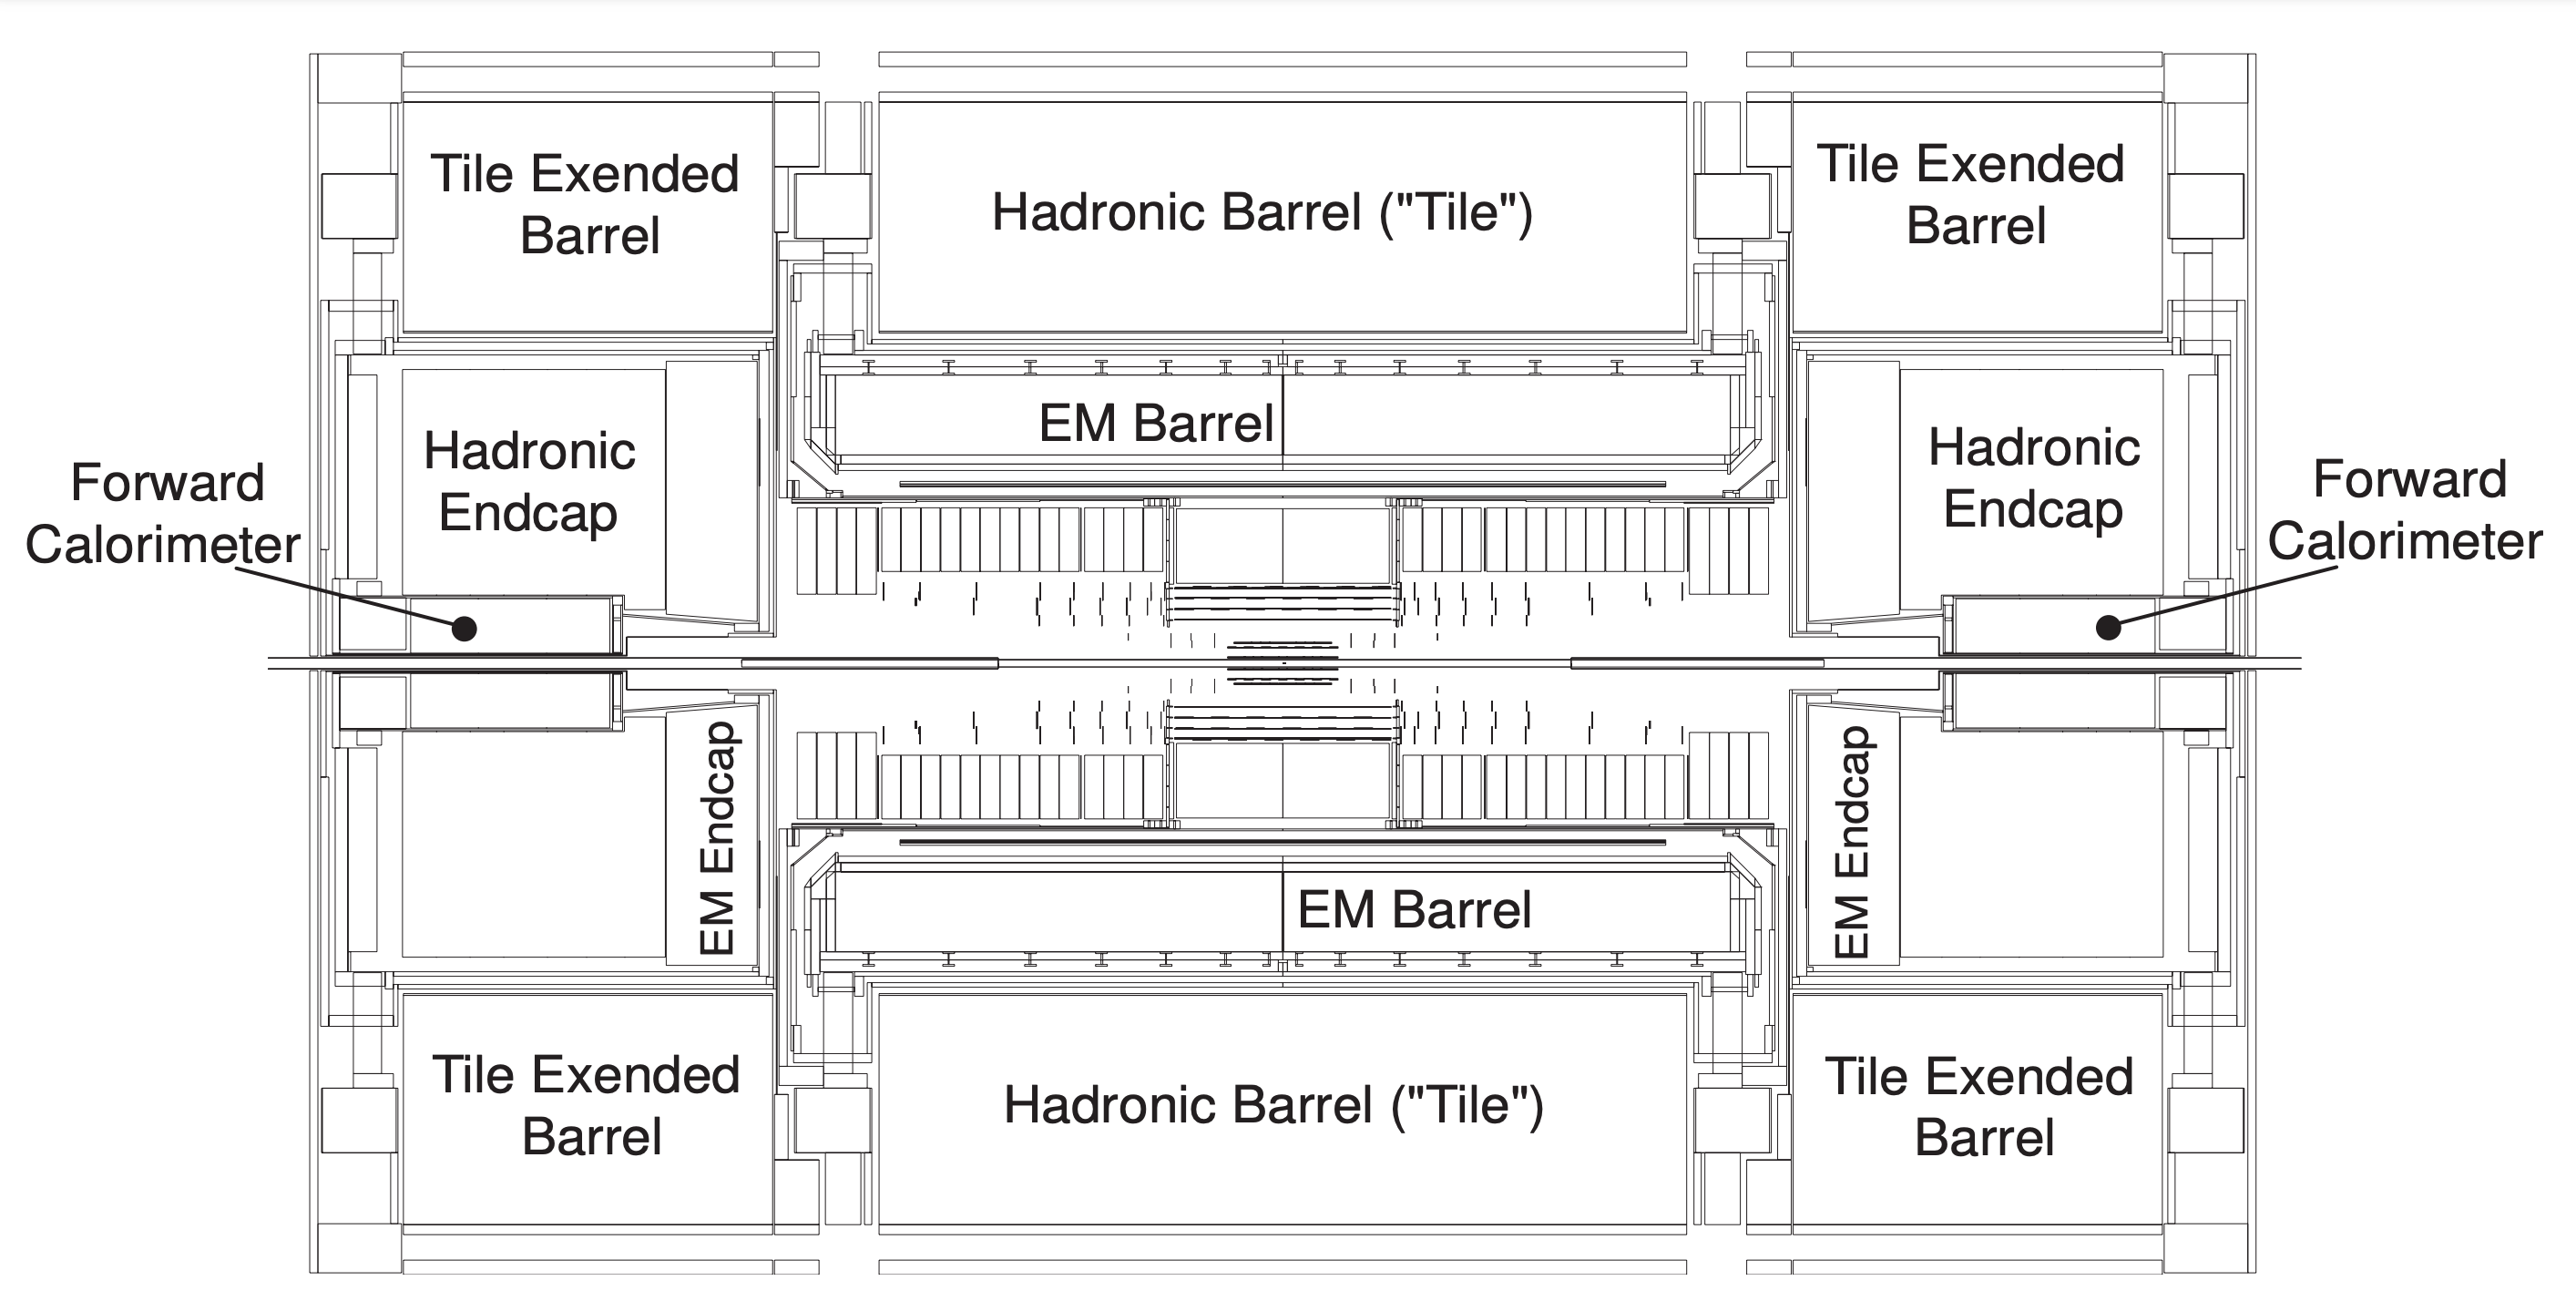
\includegraphics[width=0.99\textwidth]{Figures/LHC/ATLASCalorimetry.png}
    \caption{Cross-sectional view of the calorimetry system in the ATLAS detector. This figure is from Ref.~\cite{Lampl:923625}.}
    \label{fig:calorimeters}
\end{figure}

\subsubsection{The Electromagnetic Calorimeter}
The electromagnetic calorimeter wraps immediately around the inner detector as illustrated in Figure \ref{fig:calorimeters}. The material used for the active sensing medium is liquid Argon (LAr), chosen for its high intrinsic uniformity, long-term stability of signal response, as well as radiation hardness~\cite{Zhang_2011}. Lead plates are used as absorbers, chosen for its high hadronic interaction length to radiation length ratio. The resulting electromagnetic calorimeter has a total thickness that covers 22 times the radiation length, which corresponds to less that one hadronic interaction length, preventing hadronic showers from forming. The liquid Argon and lead layers and arranged in an accordian-like geometry, ensuring a full azimuthal coverage with minimal gaps in acceptance \todo{Find a figure? Can't seem to visualise how this helps}. The barrel sector consists of three layers of varying granularity and has coverage up to $|\eta| < 1.475$. 

The first layer has a granularity of $\Delta\eta\times\Delta\phi=0.0031\times 0.098$. The high $\Delta\eta$ resolution acts as a powerful discriminator between showers originating from single isolated photons and those originating from multiple photons, from decays of neutral mesons within jets \todo{Read more about this}. The second layer is the thickest of the three, and it absorbs the vast majority of the shower's energy. It has a granularity of $\Delta\eta\times\Delta\phi=0.025\times 0.025$. Lastly, a thinner, lower-granularity final layer with $\Delta\eta\times\Delta\phi=0.05\times 0.025$ is used to estimate the energy that leaks beyond the electromagnetic calorimeter and into the hadronic calorimeter. In order to correct for energy lost by electrons and photons when they interact with the inner detector and magnet, a liquid Argon pre-sampler is installed upstream of the calorimeter. The pre-sampler is one single sensitive layer of liquid Argon and covers the range $|\eta| < 1.8$. The electromagnetic calorimeter end-caps are made up of four wheels; an inner and outer wheel on either side of the interaction point. These are each divided into eight wedge shaped modules and cover the range $1.375 < |\eta| < 3.2$. Like the barrel modules, the end-cap modules consist of three layers of varying granularity.

\subsubsection{The Hadronic Calorimeter}
Hadrons lose energy through inelastic interactions with the detector medium, which result in the production of secondary strongly interacting particles, giving rise to hadronic showers\todo{Reword?}. The main purpose of the hadronic calorimetry system is to measure the energy of such hadrons. Its performance is essential for precision measurements of jets as well as reconstruction of missing energy~\cite{Aaboud:2018scw}. The hadronic calorimeter incorporates modules of varying technologies, the barrel region hosts a tile calorimeter and the end-caps host a liquid-argon hadronic calorimeter. 

The Tile Calorimeter, covering the central region of ATLAS, is further separated into two sub-detectors. In the $|\eta| < 1.0$ region there is the hadronic tile barrel, and the extended tile barrel resides between $0.8 < |\eta| < 1.7$. Both regions use alternating tiles of steel absorbers and scintillating sensing elements, arranged parallel to the beam axis. A total of 64 modules wedge together to give full azimuthal angle coverage. In the transverse direction there are three layers of varying granularity. The first and second layers have resolution $0.1 \times 0.1$ in $\Delta\eta\times\Delta\phi$, and the third layer a coarser resolution of $\Delta\eta\times\Delta\phi = 0.2 \time 0.1$. As an ionising particle crosses the scintillating medium, ultraviolet scintillation light is produced. Using wavelength-shifting optical fibers, this light is collected and converted into visible light. Next it is guided towards photomultiplier tubes at the top of each module, where the optical signal is measured.

The hadronic end-cap calorimeter is a liquid argon sampling calorimeter, similar to the electromagnetic counterpart. The coverage reaches the $1.5 < |\eta| < 3.2$ range in the forward region, where the more radiation resistant liquid argon technology is better suited than a tile calorimeter. The absorber in the hadronic end-cap, however, is copper rather than lead. Each end-cap consists of two separate wheels. The inner wheel has 8.5 millimetre liquid argon gaps wedged between 25 millimetre thick copper plates, whereas for the outer wheel the copper is 50 millimetre thick. The granularity is $0.1 \times 0.1$ in $\Delta\eta\times\Delta\phi$ for $1.5 < |\eta| < 2.5$, and $\Delta\eta\times\Delta\phi = 0.2 \times 0.2$ for $\Delta\eta\times\Delta\phi$ for $2.5 < |\eta| < 3.2$.

%%The Tile barrel measures 5.8 m in length, whereas the two extended barrels 2.8 m each. Both systems have an inner radius of 2.28 m and an outer radius of 4.25 m. 


\subsection{The Muon Spectrometer}
\label{ssec:ATLASMS}
The outermost layer of the \ATLAS detector system is the muon spectrometer, which as the name suggests, is designed to provide efficient, high-resolution measurements of muons' trajectory and momenta. Energetic muons are minimum ionizing particles, and can penetrate through the calorimeters. Installing this tracking system wrapping around the other sub-detectors gives muons a very distinctive detector signature, leading to a high purity and efficiency in their reconstruction. Figure \ref{fig:muonspectrometer} shows the layout of the muon system, which consists of four gaseous tracking chambers installed between the eight coils of the barrel toroidal magnetic system, as well as before and after the toroid magnets of the endcaps. Two of these are precision tracking chambers made for precision momentum measurements, and the other two act as an efficient trigger system for fast response \cite{PALESTINI2003337}. 

\begin{itemize}
    \item Monitored Drift Tubes (MDT): To provide precision coordinate measurements in the bending plane of the the muon spectrometer, Monitored Drift Tube (MDT) chambers are installed over the full pseudorapidity range $|\eta| < 2.7$. Each MDT component consists of a 3 cm diameter pressurised aluminium drift tube filled with 93\% argon and 7\% carbon dioxide gas at three bar \cite{LEVIN2008347}. As a muon passes through a drift tube, ionisation electrons drift towards the centre where a wire stretches through the longitudinal axis. 
    \item Cathode Strip Chambers (CSC): The number of MDTs is reduced in the forward region $2.0 < |\eta| < 2.7$, where particle flux is twenty times higher than the average in the rest of the MS. Here, Cathode-Strip Chambers (CSC) aid momentum measurement. The CSC are multi-wire proportional chambers, with the cathode segmented into strips, and the direction of the strip is perpendicular to one of the wires. This allows for two independent measurements of the muon: one for the ionisation electrons that are collected at the wire, the other one from the induced signal collected at the strips. \change[]{Read more about this} %reword, this is copy pasted.}
    \item Resistive Plate Chambers (RPC): Installed in the barrel region, these chambers provides fast tracking in the $\eta<1.05$ region. Each chamber is made up of two gaseous volumes, Bakelite plates, and read-out electronics \cite{PALESTINI2003337}. 
    \item Thin Gap Chambers (TGC): Installed in the endcaps, TGCs makes up the second part of the muon trigger system. In total each endcap has seven layers \todo{Is it 7 or 9 layers? Find a citation.} of TGC. Each layer is made up of two resistive grounded cathode planes, with a sheet of closely spaced wires sandwiched inside \cite{Etzion}. A positive high voltage is applied to the wire anode. The gap between the anode to cathode plane is thinner than the wire to wire spacing (\unit{1.4}{\milli\meter} and \unit{1.8}{\milli\meter} respectively), a characteristic reflected in the name of these chambers. TGCs act as a level-1 trigger, and provide high efficiency and excellent time resolution in a high-background environment \cite{NAGAI1996219}.

    %This feature in combination with a highly-quenching gas mixture of n-pentane and CO2 allows fast and safe operation at high particle flux. The signal read from the wires provides a bending direction position measurement with a few-mm accuracy. Copper strips separated from a graphite cathode plane by a flameresistant material layer provide an azimuthal measurement with a similar accuracy. 
\end{itemize}
\begin{figure}
    \centering
    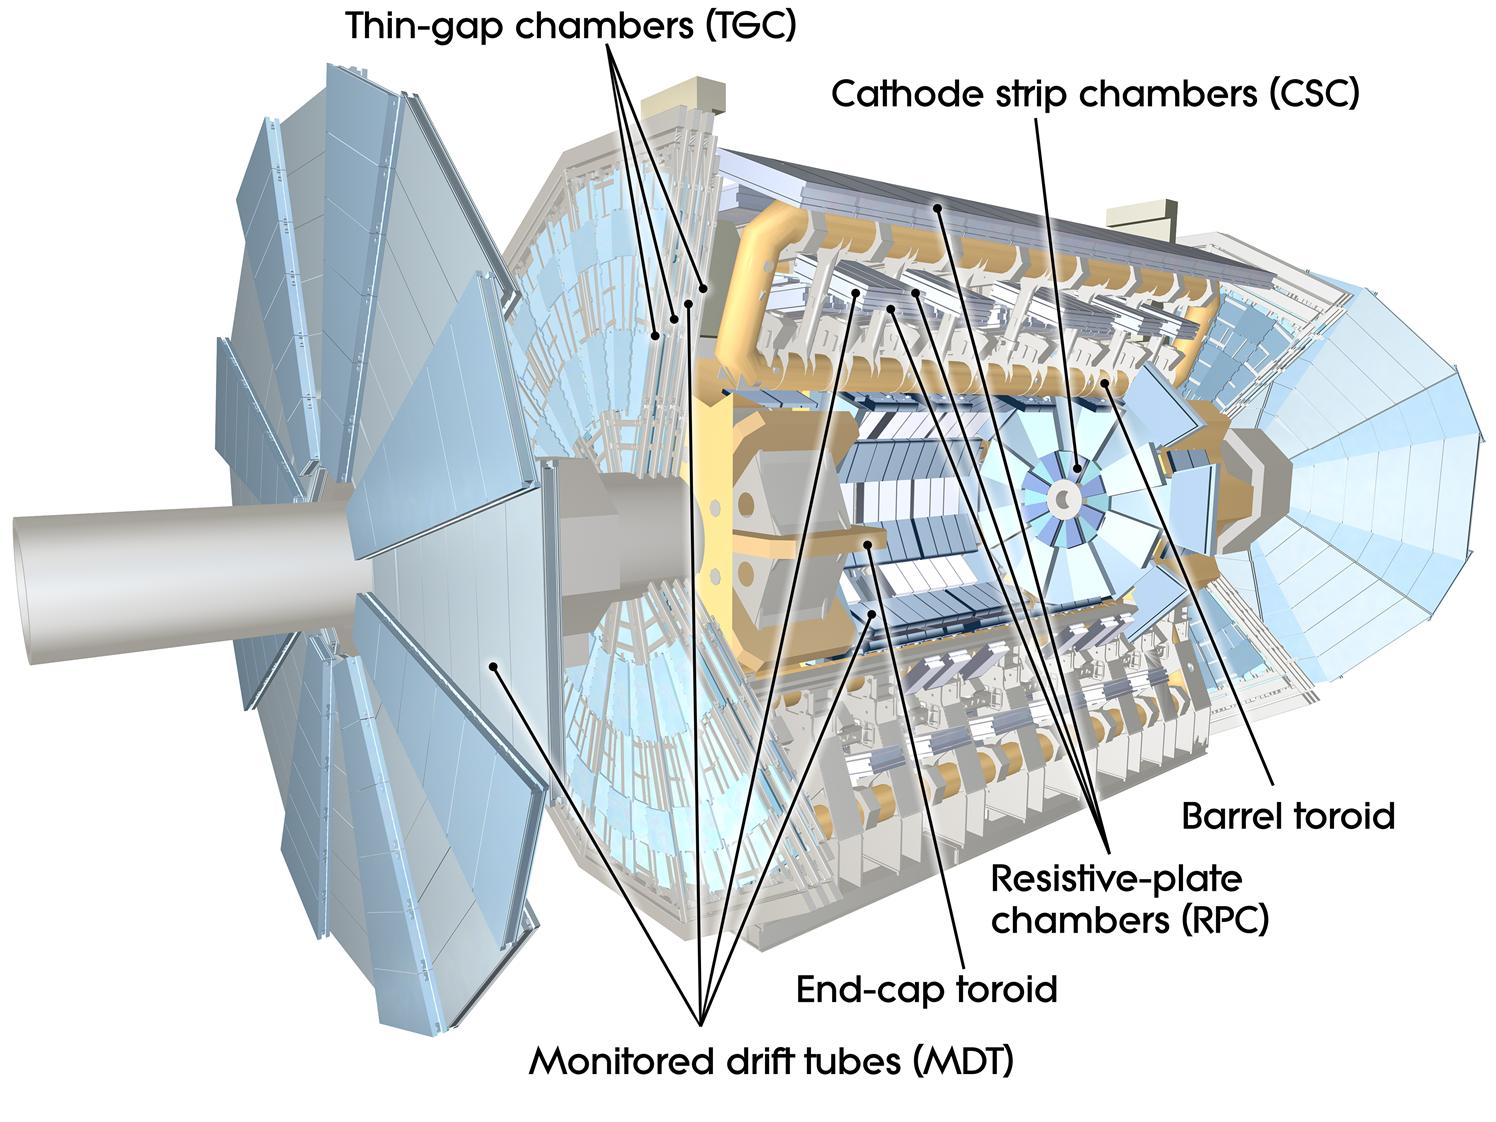
\includegraphics[width=0.8\textwidth]{Figures/LHC/ATLAS_MS.jpeg}
    \caption{A section view of the ATLAS Muon Spectrometer and its sub-components. This figure is from Ref.~\cite{ATLAS_MS}}
    \label{fig:muonspectrometer}
\end{figure}
\subsection{Magnet system}

The ATLAS detector incorporates a powerful magnet system that bends the trajectory of charged particles in order to measure their momentum with high accuracy. The momentum is deduced via the radius of curvature of the tracks seen within the detector systems. A pictorial representation of the ATLAS magnet system is shown in Figure \ref{fig:atlasmagnets}. It is a system comprised of four separate superconducting magnets - one barrel toroid and two endcap toroids incorporated in the muon spectrometer, and one central solenoid surrounding the inner detector. All four magnets are indirectly cooled, through conducting, by circulating helium at 4.5 K in the tubes welded onto the aluminum structure that encloses the coils \cite{828245}. 

The central solenoid is cylindrical in shape, and designed with minimal thickness in order to reduce energy loss before the particles enter the calorimeter. It is a superconducting magnet constructed from niobium-titanium alloy. It provides a magnetic field of \unit{2}{\tesla} to the inner detector axially (parallel to the $z-$axis), deflecting charged tracks along the $\phi$ coordinate. The strength of the central solenoid's magnet field is near constant along the radial direction, however it decreases on the axial edges due to the finite length of the magnet. 

The air toroid system is composed of three magnets: one forming a barrel section, and the others two end-caps. Each is composed of eight coils positioned in azimuthal symmetry around the beam axis. The toroids bend charged particles in the muon spectrometer. Unlike the central solenoid, however, the magnetic field strength varies. In the barrel it is between 0.15 Tesla and 2.5 Tesla, and in the endcaps it starts at 0.2 Tesla and reaches up to 3.5 Tesla \todo{Check these values and cite}. The toroids' generated magnetic fields are orthogonal to that of the solenoid. This has the advantage that independent measurements of muon momenta can be made in the inner- and outer-most regions of the detector.

\begin{figure}[htb!]
    \centering
    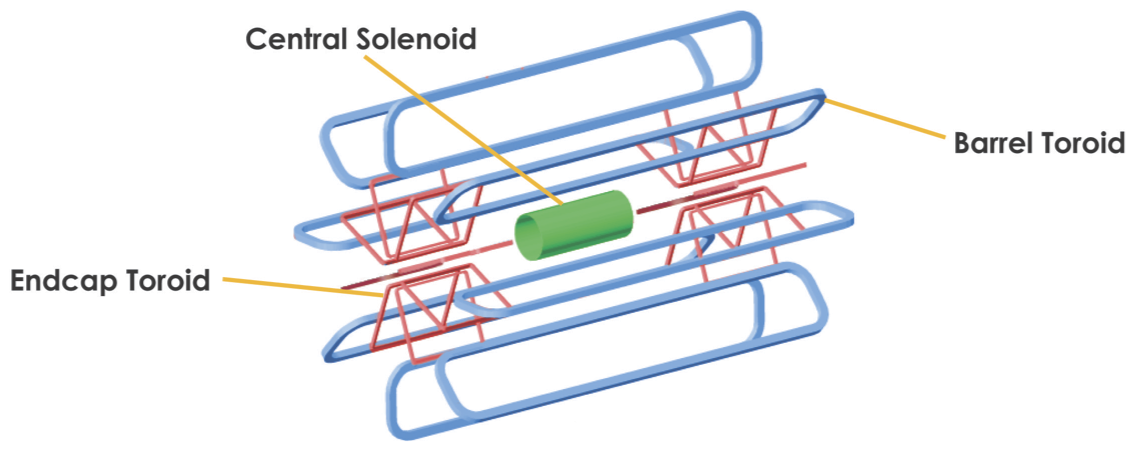
\includegraphics[width=0.7\textwidth]{Figures/LHC/exp-magnets.png}
    \caption{Schematic representation of the ATLAS magnet system. This Figure is from Ref.~\cite{atlasmagnet}.}
    \label{fig:atlasmagnets}
\end{figure}

\subsection{Trigger system}
\label{ssec:ATLAStrigger}
ATLAS does not record every single collision that the LHC produces. This is partially because most events are uninteresting low-energy processes, and partially because the amount of bandwidth and computing resources required make it impossible to do so. During run 2 the LHC had a bunch crossing rate of twenty five nanoseconds, corresponding to a collision frequency of forty megahertz. That's on the order of a few thousand gigabytes of data per second! It is neither feasible or practical to read out and record data at this frequency, and here the nifty trigger system comes into play. The ATLAS triggers act like a fine sieve and select only rare, interesting events. Typically, interesting events involve objects that have high momentum or energy in the transverse direction. The ATLAS trigger system throughout run 2 effectively reduces the crossing rate from forty megahertz to one kilohertz through two triggers. The first is the level-1 (L1) trigger, a hardware based trigger that uses coarse objects from the calorimeters and the muon spectrometer, which reduces the rate to 100 kilohertz. The second is a software based high level trigger (HLT), which makes further selection choices bringing the final rate to one kilohertz~\cite{zurNedden:2238679}. 

\subsubsection{Level-1 trigger}

The level-1 trigger consists of several subsystems. The level-1 calorimeter (L1Calo) and level-1 muon (L1Muon) subsystems operate separately with calorimetry and muon spectrometry information. The L1Calo trigger receives reduced resolution analogue signals from calorimeter trigger towers. These are formed by $\eta\times\phi=0.1\times0.1$ regions in the barrel and $\eta\times\phi=0.4\times0.4$ regions in the endcaps~\cite{pdg_2021}, separately for the electromagnetic and the hadronic calorimeter~\cite{Aad:2716326}. In the central region $|\eta| < 3.2$, L1Calo uses a sliding window algorithm to search for local maximum and forms regions of interests (ROIs) around them, which are sent for further processing to the HLT. L1Muon looks for coincident hits in the muon spectrometer; more specifically in the resistive plate chambers of the barrel region and and thin gap chambers in the endcaps, see Section~\ref{ssec:ATLASMS}. Finally there is the level-1 topological trigger (L1Topo), which makes use of takes trigger objects from both L1Calo and L1Muon and combines them into topological information. For example, one can require that two leptons have small angular separation $\Delta R < 0.1$. The L1 trigger makes a binary accept or reject decision via the the central trigger processor (CTP) which takes input from the three L1 subsystems. The acceptance rate reaches up to \unit{100}{\kilo\hertz}, and the data latency is \unit{2.5}{\micro\second}. 

\subsubsection{High level trigger}

Once the level-1 trigger has accepted an event, it passes the baton onto the software-based high level trigger (HLT) for processing. The HLT uses the ROIs provided by the L1 trigger to seed regional event reconstruction with full detector granularity, including tracking information from the inner detector. Upon receiving an accept signal from the L1 trigger, the front-end electronics sent data out to the readout system via readout drivers. Reconstructing events is computationally expensive, thus the HLT is a built as a series of numerous individual trigger chains. At each stage an event may be rejected should it fail to meet the criteria of the chain. Rejected events are aborted, avoiding the need to run more CPU intensive algorithms. Once the HLT decides to accept an event, the full event data from various detectors are gathered and transferred to the tier-0 facility at CERN for preliminary analysis. The final event acceptance rate is reduced to an average of \unit{1.5}{\kilo\hertz}, a much more bearable 1.5 GB per second~\cite{zurNedden:2238679}. Not all triggers need run, or indeed can run, at their full rate. Here the trigger prescales come into play. The prescale value determines the fraction of events an HLT algorithm is being executed on, including when it is deactivated. This feature is both essential during the commissioning phase of the HLT as well as for adjusting the mixture of recorded physics events during an LHC run~\cite{Winklmeier}. 

\section{Object reconstruction}

The \ATLAS detector's raw readout signals must be translated into meaningfiul physics information before delivered to analysis teams. The responsibility for this task falls upon the offline reconstruction system, which combines information from all sub-detectors to reconstruct and identify particles with the highest possible efficiency. 

\subsection{Tracks and vertices}
\label{ssec:tracksandvertices}

Reconstruction of complex physics objects, such as electrons and muons, begins with the construction of more basic inputs such as tracks, vertices, and calorimeter clusters. 
Charged particle trajectories are called tracks, and their reconstruction is crucial for many reasons. They are explicit inputs in the identification, reconstruction and isolation of electrons and muons, which is the signal process for the analysis of this thesis. The basic building block of a track is the detection of a signal above threshold, a hit, in the inner tracking detectors. In the pixel detector and semi-conductor tracker, the hits are first assembled into clusters of energy deposits that share common corners and edges, called space points. Tracks are seeded with a triplet of space points and are extended by matching subsequent pixel and SCT hits. This is done using a Kalman filter~\cite{ATLAS-CONF-2012-042}, which searches for adjacent clusters both outwards and inwards in the radial direction while attempting to smooth the trajectory.

When describing a track, five parameters are used: $d_0$ and $z_0$, the transverse and longitudinal impact parameters, $\phi$ and $\theta$, the azimuthal and polar angle, and $q/p$ describing the charge~\cite{Akesson:973401}. Together these are known as the perigee parameters. The two impact parameters are illustrated in figure \ref{fig:impactparameters}. The transverse $d_0$ is the transverse distance from the primary vertex to the point of closest approach in the $\eta-\phi$ plane, while the $z_0$ is the distance  from the $z-$axis. 
\begin{figure}
    \centering
    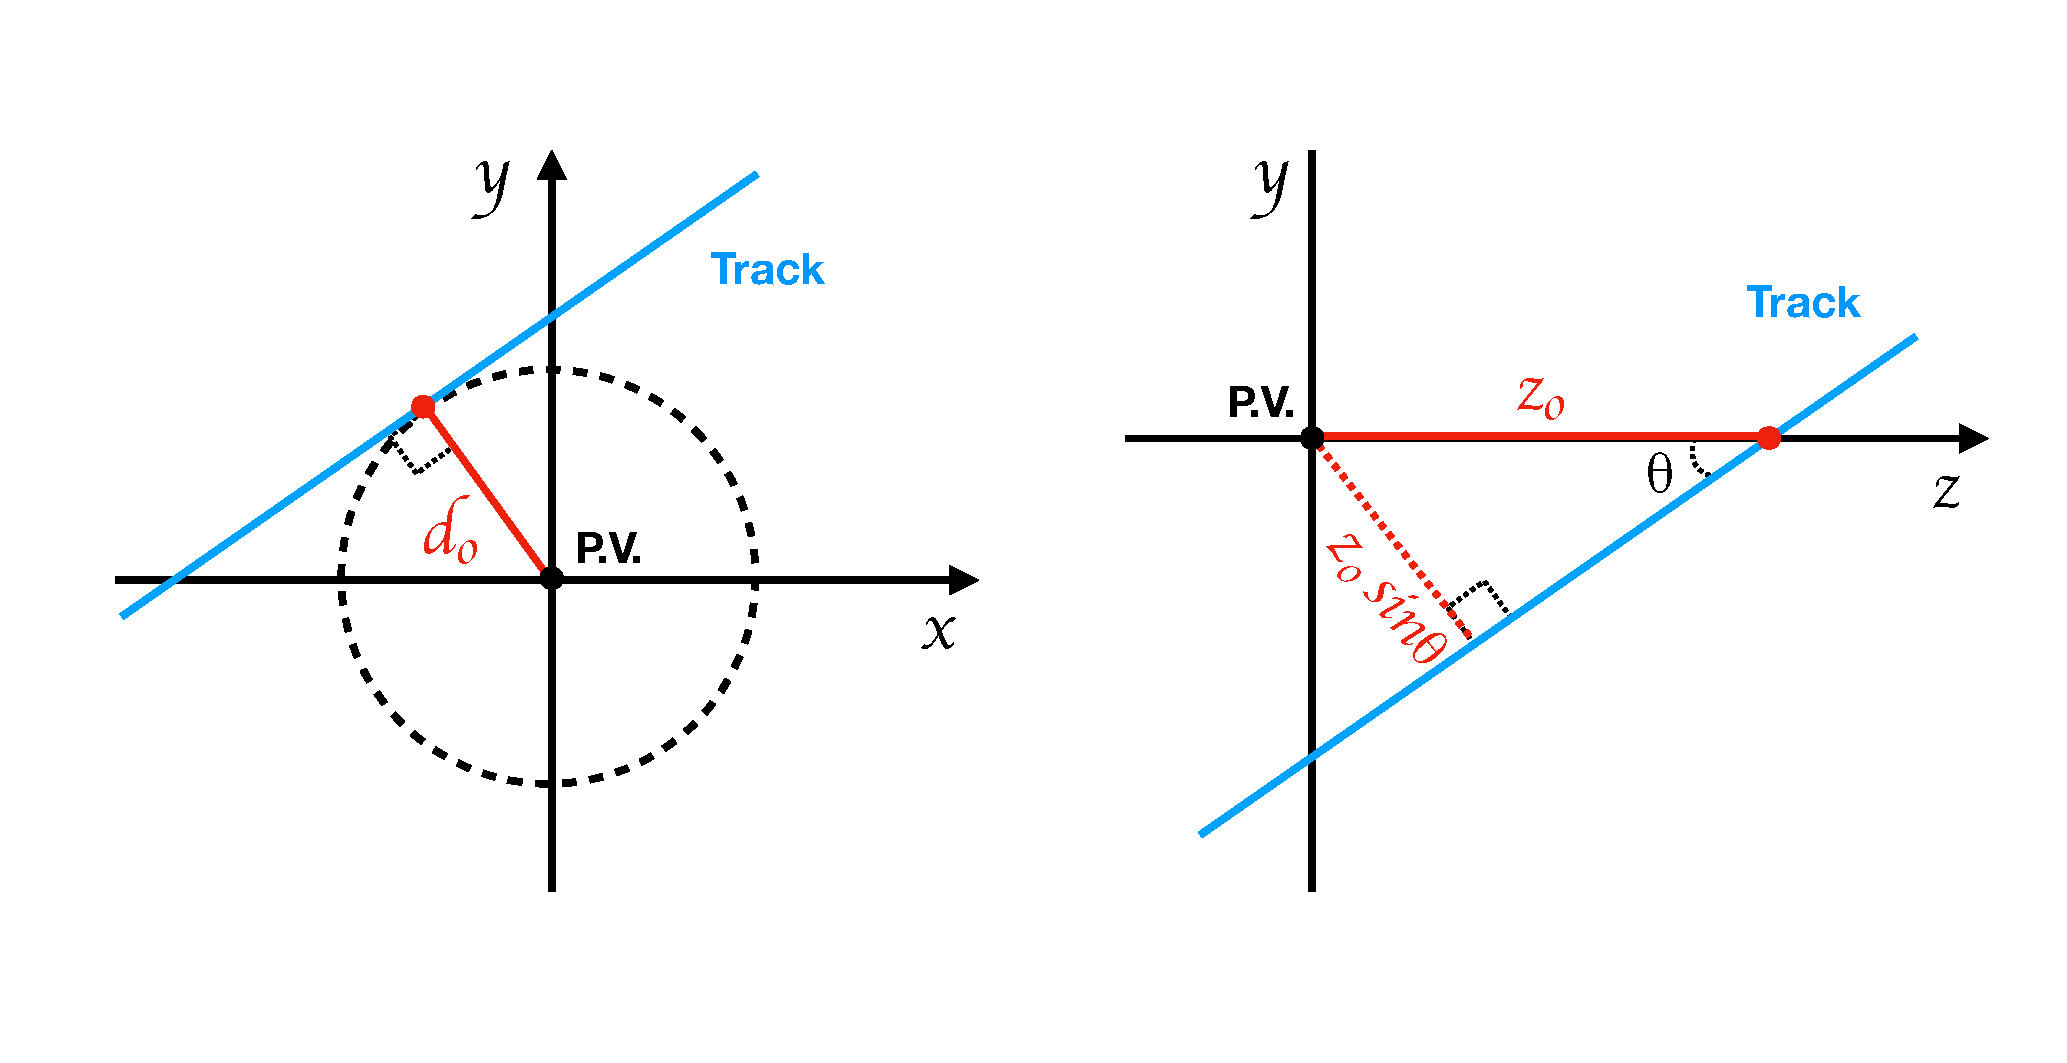
\includegraphics[width=\textwidth]{Figures/LHC/impact_params.pdf}
    \caption{Drawn in blue is the particle track, with the transverse and longitudinal impact parameters illustrated on the left and right graph respectively. The primary vertex (P.V.) is defined to be at the origin.}
    \label{fig:impactparameters}
\end{figure}
The momentum can be deduced from the track using the radius of curvature and the solenoid field strength. High momentum particles have less curved trajectories than low momentum particles. The collision vertex is the intersection of multiple particle trajectories at their origin. For vertex finding at least two reconstructed tracks are required as input. The primary vertices are points in space where proton–proton interactions have occurred \cite{ATLAS_primary_vertices}. Track to vertex association is split into two stages: 
\begin{itemize}
    \item Vertex finding associates reconstructed tracks to potential vertex candidates
    \item Vertex fitting is the reconstruction of the vertex position, as well as an estimate on the quality of the fit \cite{Piacquadio_2008}.
\end{itemize}
These two steps are often interlaced in the algorithms. With a set of selected tracks and a vertex seed position, an iterative procedure is used to find the best vertex position. After the vertex position is computed, incompatible tracks are removed and regrouped with the non-selected tracks to be used in finding and fitting or another vertex. 

\subsection{Clustering algorithms}
\label{ssec:clusteringalgorithms}
In the calorimeters, the signals are collected into related clusters. This is done to extract the significant signal coming from the hard scattering process from the noise \cite{Aad_2017_topo_clustering}. In the calorimeters, the noise arises from two main sources: the readout electronics, and pile-up from non-primary interactions \cite{Lampl:1099735}. The clustering algorithms aim to group together the calorimeter cells, in three dimensions, in which incoming particles have deposited their energy. The clustering allows for the computation of the sum of the total energy deposited. Within \ATLAS, there are two clustering algorithms: the sliding-window algorithm, and the topological algorithm. Both are summarised below and are described in detail in reference \cite{Lampl:1099735}. 

\subsubsection{Sliding-window algorithm}

The sliding-window algorithm first divides the $\eta-\phi$ space into a grid. All longitudinal cells' energies in each grid element is summed together to form rectangular prisms called towers. Next, a fixed sized window of $N_{\eta}\times N_{\phi}$ towers is used to scan across the grid in search of a local maximum above a chosen energy threshold. once found, it is used as a seed for the final step; cluster formation. Depending on the hypothesised particle type and the location in the calorimeter, the clusters pre-defined size in $\eta-\phi$ space varies \cite{Lampl:1099735}. Clusters are built by summing the energies of all cells within the defined size.

In cluster formation, the sliding window algorithm can form overlapping clusters if they share common cells. In these cases, the reconstruction algorithm (by default) includes the overlapping cells in both clusters, thus resulting in a double count of the energies of the shared cells. The disadvantage of this approach is that objects can be reconstructed with a larger energy that it had initially, due to the double counting. 

\subsubsection{Topological clustering}

Unlike the sliding-window algorithm, topological clustering results in clusters that have variable cell sizes. The building of clusters starts by examining the cell signal significance $\zeta_{\text{cell}}$, defined as
\begin{equation}
    \zeta_{\text{cell}} = \dfrac{E_{\text{cell}}}{\sigma_{\text{noise,cell}}}
\end{equation}
where the numerator is the energy deposited in the cell and the denominator is the average expected noise in the cell \cite{Aad_2017_topo_clustering}. In building the topological clusters, three thresholds are defined. The seed threshold $\zeta_{\text{seed}}$, the neighbour threshold $\zeta_{\text{neighbour}}$, and the baseline cell threshold $\zeta_{\text{base}}$. Any cell whose cell significant is above the seed threshold is labelled as a seed cell, and forms a proto-cluster. The seed cells are ranked from high to low based on their $\zeta_{\text{cell}}$ value. From there, neighbouring cells that have not been used as a seed cell are added to the proto-cluster if their energy is above $\zeta_{\text{neighbour}}$, and also added to the neighbour seed list. If a neighbour cell is next to two proto-clusters, then the proto-clusters are merged. If $\zeta_{\text{cell}}$ is below $\zeta_{\text{neighbour}}$ but still above $\zeta_{\text{base}}$, then the cell is added to the nearest neighbouring proto-cluster. After the original seed list is processed, it is discarded and the same procedure is repeated for neighbour seed list. This is done until no cells remain unprocessed. 

The advantage to the topological clustering method, as opposed to the sliding window method, is that it allows for a more organic growth of clusters rather than pre-defining its size and shape. The algorithm is formed so that it closely traces the spatial signal-significance
patterns generated by particle showers \cite{ATL-PHYS-PUB-2017-022}. Furthermore, topological clustering requires smaller energy loss corrections. It has a very efficient energy resolution and collects more energy on average than sliding window clustering \cite{ATL-PHYS-PUB-2017-022}. It is more complex to implement, however, and due to the dependency on noise levels, uncertainties from the electronics and pile-up directly affect the algorithm's reconstruction efficiency \cite{Lampl:1099735}. 

In reference \cite{ATL-PHYS-PUB-2017-022}, a topological clustering algorithm for electron and photon reconstruction is presented. It is demonstrated that this algorithm improves the energy resolution when compared to the traditional sliding window method. Figure \ref{fig:H4l_topo_cluster} shows the resolution improvements in the \HFourL{} channel, taken from reference \cite{ATL-PHYS-PUB-2017-022}. The topological cluster approach has a more narrow Higgs peak, and the peak is also closer to the true Higgs mass. After performing a fit with a double Crystal Ball function, the $4e$ channel shows a 5\% improvement in resolution.
\begin{figure}
    \centering
    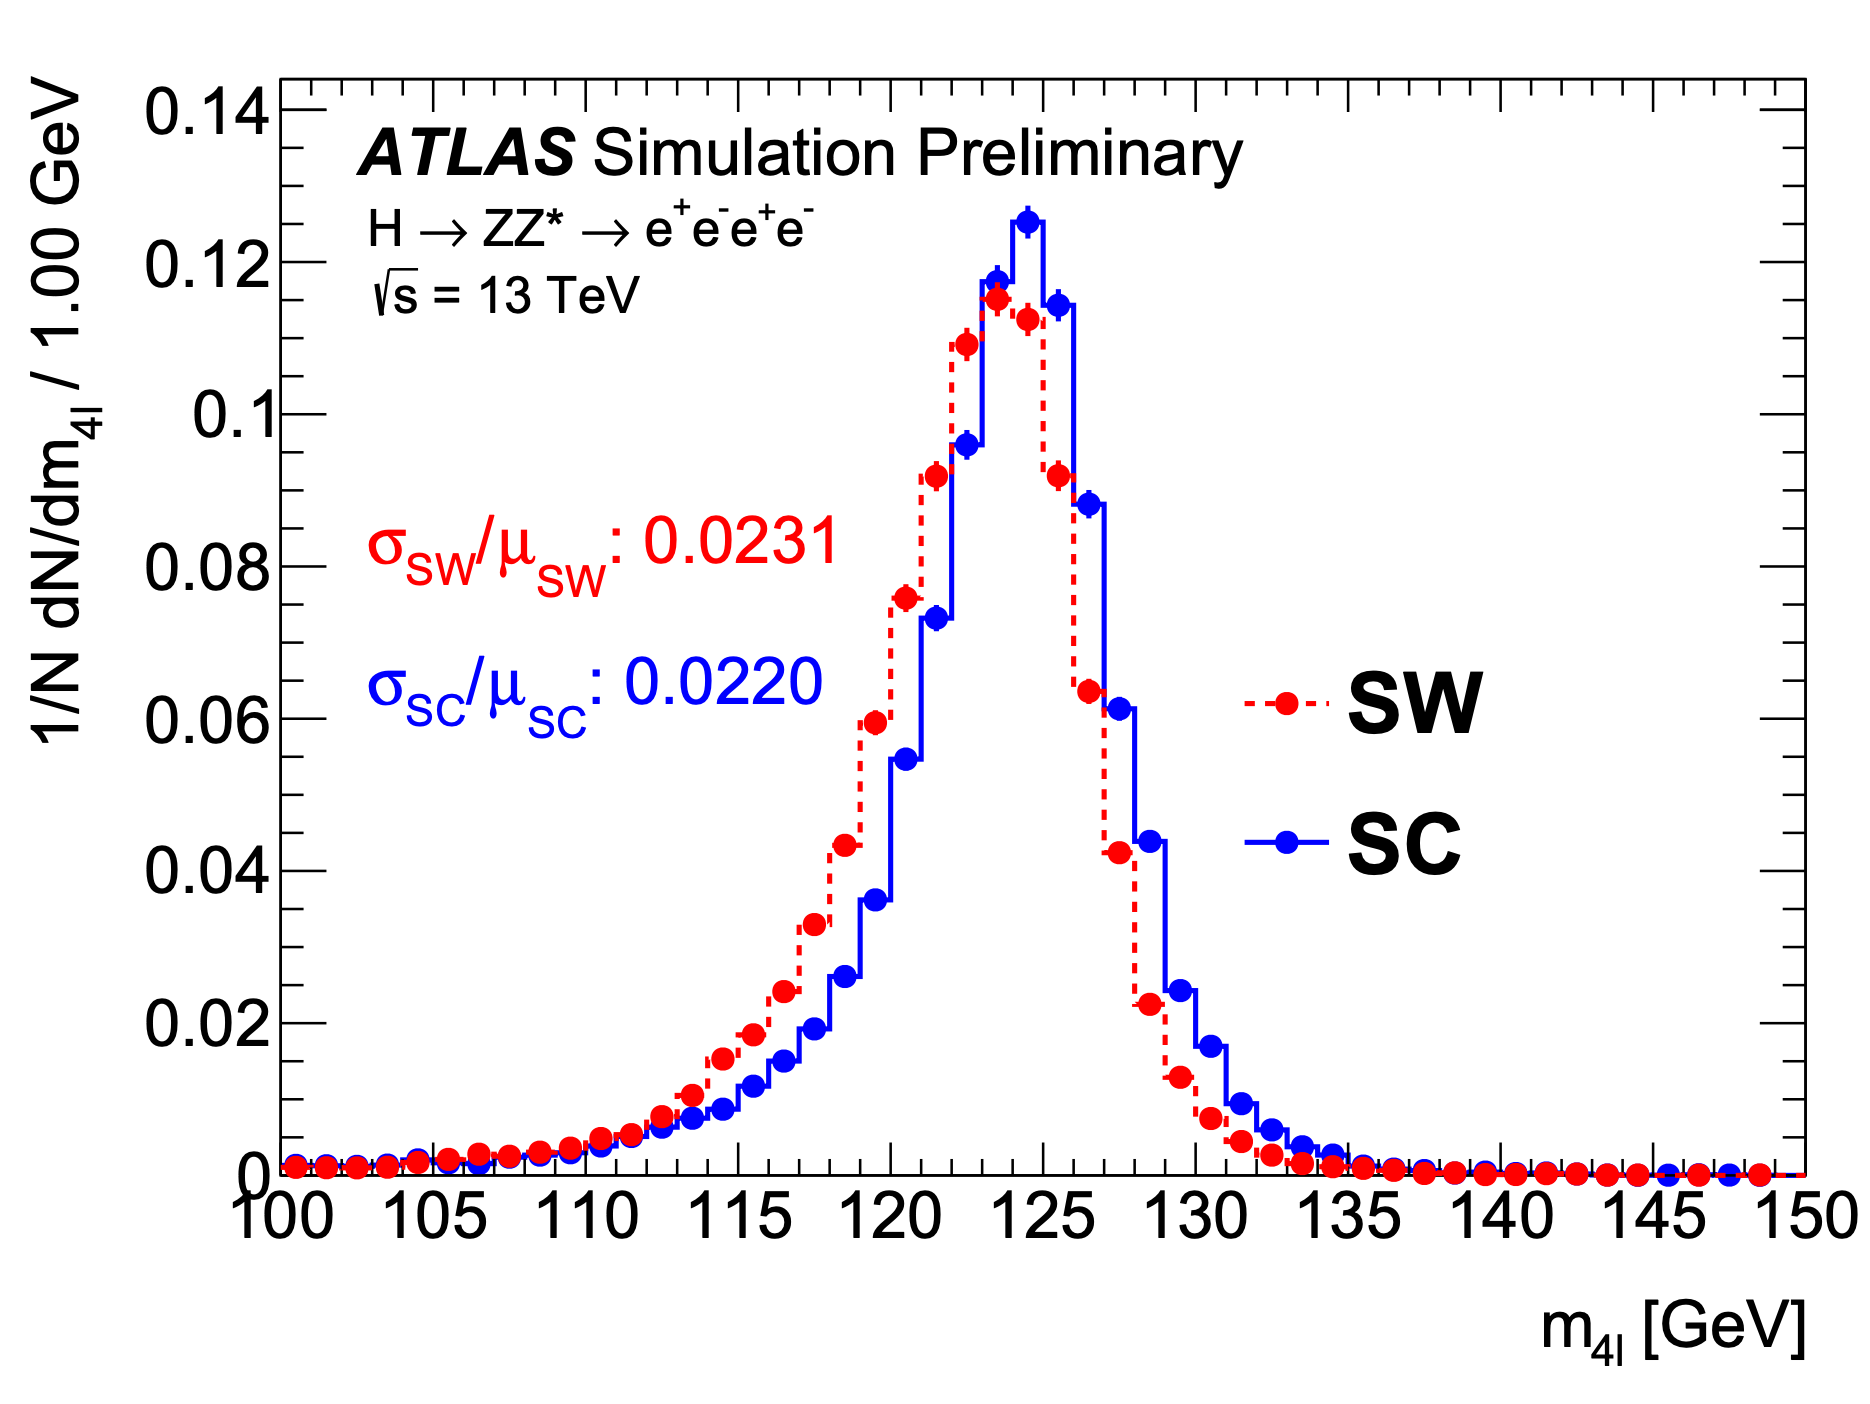
\includegraphics[width=\mediumfigwidth]{Figures/LHC/H4l_topo_cluster.png}
    \caption{Simulated 4 lepton invariant mass distributions using the super-cluster (SC) and sliding window (SW) algorithms, in the $4e$ channel. This figure is from Ref.~\cite{ATL-PHYS-PUB-2017-022}.}
    \label{fig:H4l_topo_cluster}
\end{figure}

\subsection{Electrons}
\label{ssec:electronreco}
\subsubsection{Electron reconstruction}

Following track candidate and calorimeter cluster candidate reconstruction as described in sections \ref{ssec:tracksandvertices} and \ref{ssec:clusteringalgorithms} comes the final procedure in electron reconstruction: the matching of a track candidate to a topo-cluster and the finalisation of the cluster size \cite{ATLAS_electron_efficiency_2015-2016}. The algorithm prepares for reconstruction by first selecting the topo-custers and tracks it will use. The tracks are then refitted  using a Gaussian sum filter (GSF) method \cite{ATLAS-CONF-2012-047} to accommodate for the energy loss due to bremsstrahlung radiation, which affects electrons more significantly than muons due to their lighter mass. As an electron loses its energy, its transverse momentum also decreases, and the curvature of its track becomes more prominent. The refit improves electron reconstruction efficiencies by correcting for this effect and improving the track parameters.

By extrapolating the track from the perigee to the second calorimeter layer and using the track's momentum, re-fitted tracks are matched to topological clusters. Sometimes the momentum of the track is rescaled to match the energy of the cluster, which improves matching accuracy for electron candidates that lose a portion of their energy to bremsstrahlung radiation \cite{ATLAS_electron_efficiency_2015-2017}. In order for a track to match, the requirements $|\Delta\eta|<0.05$ and $-0.10<q\cdot(\phi_{\text{track}}-\phi_{\text{cluster}})<0.05$ must be fulfilled, where $q$ is the charge of the track. The asymmetry of the latter requirement is due to radiated photons which clusters are able to measure, but tracks may miss \cite{ATLAS_electron_efficiency_2015-2017}.

\subsubsection{Electron identification}

Electron identification is done using a likelihood method that takes calorimeter shower shapes, tracking information, and cluster-track matching information as inputs. The advantages of this approach, as opposed to a cut-based approach, are twofold. The first is that a prompt electron may fail to be identified if it does not pass a singular selection criterion for cut-based identification. In a likelihood-based method, however, the electron may still be identified. Secondly, discriminants that are too similar to be used in a cut-based approach (because it would result in drops in efficiency) are easily added to the likelihood-based approach without penalty \cite{ATLAS_electron_efficiency_2015-2016}.

The ATLAS experiment carries out many physics analyses which require different signal efficiencies and background rejection rates. For this reason, the likelihood-based discriminant takes on fixed values for discrete working points \cite{ATLAS_electron_efficiency_2015-2016}. These working points are namely loose, medium, and tight, each corresponding to increasingly stringent thresholds. In Run 2, the electron candidates satisfying the tigher criteria are a subset of those satisfying the looser criteria. The efficiencies are 93\%, 88\%, and 80\% for identifying a \unit{40}{\GeV} electron in the loose, medium, and tight working points respectively. The medium and tight operating points have lower efficiencies and consequently a factor of 2.5 and 5 times higher fake electron rejection rates, respectively. 

For the ATLAS four lepton analysis of this thesis, the Loose electron identification working point is chosen following the studies of the \HFourL{} analysis \cite{ATLAS_H4l_2015}. In terms of tracking criteria, this requires a minimum of two hits in the pixel detector, and seven total hits in the pixel and SCT combined. The Loose likelihood selection originally made to match and improve the previous ATLAS Multilepton working point, a cut-based selection optimized for the \HFourL{} analysis \cite{ATLAS_muon_reco_2011}.

\subsubsection{Electron isolation}

Isolation is an important step in distinguishing prompt electrons in signal processes, from misidentified hadrons, semi-leptonic heavy quark decays, and other such background processes. Signal processes are usually characterized as being well isolated; there is little activity in the surrounding cells of the signal object in the calorimeter and the inner detector alike. In order to quantify the amount of activity surrounding the object of interest, a cone is defined around the electron's trajectory and the signal inside that cone (excluding the electron itself) is summed. There are two types of variables considered for isolation, one that is calorimeter-based and one that is track-based \cite{ATLAS_electron_efficiency_2015-2016}. 

The calorimeter isolation, $E_{\text{T}}^{\text{iso}}$, is the transverse energy sum of topological clusters in a cone around the electron candidate. The value is fully corrected by subtracting the $E_{\text{T}}$ of the underlying event and effects from pile-up \cite{ATLAS_electron_photon_triggers_run2, ATLAS_electron_efficiency_2015-2016}. The track isolation, $p_{\text{T}}^{\text{iso}}$, is similarly obtained by taking the scalar $p_{\text{T}}$ sum of $p_{\text{T}}>1$ GeV tracks that satisfy basic quality requirements in a cone around the electron candidate. To minimise the effects from pile-up, a requirement on the product of the longitudinal impact parameter and the sine of the polar track angle, $|z_0\sin\theta|<3$ mm, is imposed \cite{ATLAS_electron_efficiency_2015-2016}. This requirement selects tracks whose vertex is also the relevant vertex of the process. 

The various working points for track isolation are described in detail in references \cite{ATLAS_electron_efficiency_2015-2016,ATLAS_electron_efficiency_2015-2017}. The leptons in the relevant analysis of this thesis use the FixedCutPflowLoose isolation working point, with $E_{\text{T}}^{\text{iso}}/E_{\text{T}}<0.2$ and $p_{\text{T}}^{\text{iso}}/p_{\text{T}}<0.15$ for electrons. 

\subsection{Muons}
\label{ssec:muonreco}
\subsubsection{Muon reconstruction}

Muons come in various types depending on the what subdetector information was used in reconstruction \cite{ATLAS_muon_reco_2015}. In total there are four classes of muons: combined, segment-tagged, calorimeter-tagged, and extrapolated. Most reconstructed muons are combined muons, indeed, these are the purest of the four identification categories with the smallest percentage of fakes. Combined muons have tracks reconstructed independently in the inner detector and the muon spectrometer, and a global refitting procedure is used to combine the tracks. Segment-tagged (ST) muons are those with a track in the inner detector that is outwards extrapolated to at least one matched track segment in the muon spectrometer. Segmented tracks occur to muons with lower momentum, and in regions of the muon spectrometer with acceptance holes. Calorimeter tagged muons refer to a muon with an identified track in both the inner detector that is matched to a MIP-like energy cluster in the calorimeter. Of all the muon types this is the one with the lowest purity. As it does not rely on the muon spectrometer, its role is to recover the coverage gap around $\eta=0$. Lastly, extrapolated muons (synonymously standalone muons) are reconstructed without an inner detector track, and are based only a full muon spectrometer track. These types are mainly used to extend the muon coverage in the high-$\eta$ region where the inner detector has no coverage. 

These four types of muons exists because muons offer an extremely clean signal in the detector, and therefore they can afford to be further categorised. Figure \ref{fig:typesofmuons} illustrates the detector profiles of each type of muon. In the high multiplicity four lepton channel, the signal is particularly sensitive to changes in lepton acceptance. For the $4\mu$ channel (the flavour channel with the highest resolution), the slightest improvement in muon acceptance will cascade into a significant overall acceptance. 
\begin{figure}
    \centering
    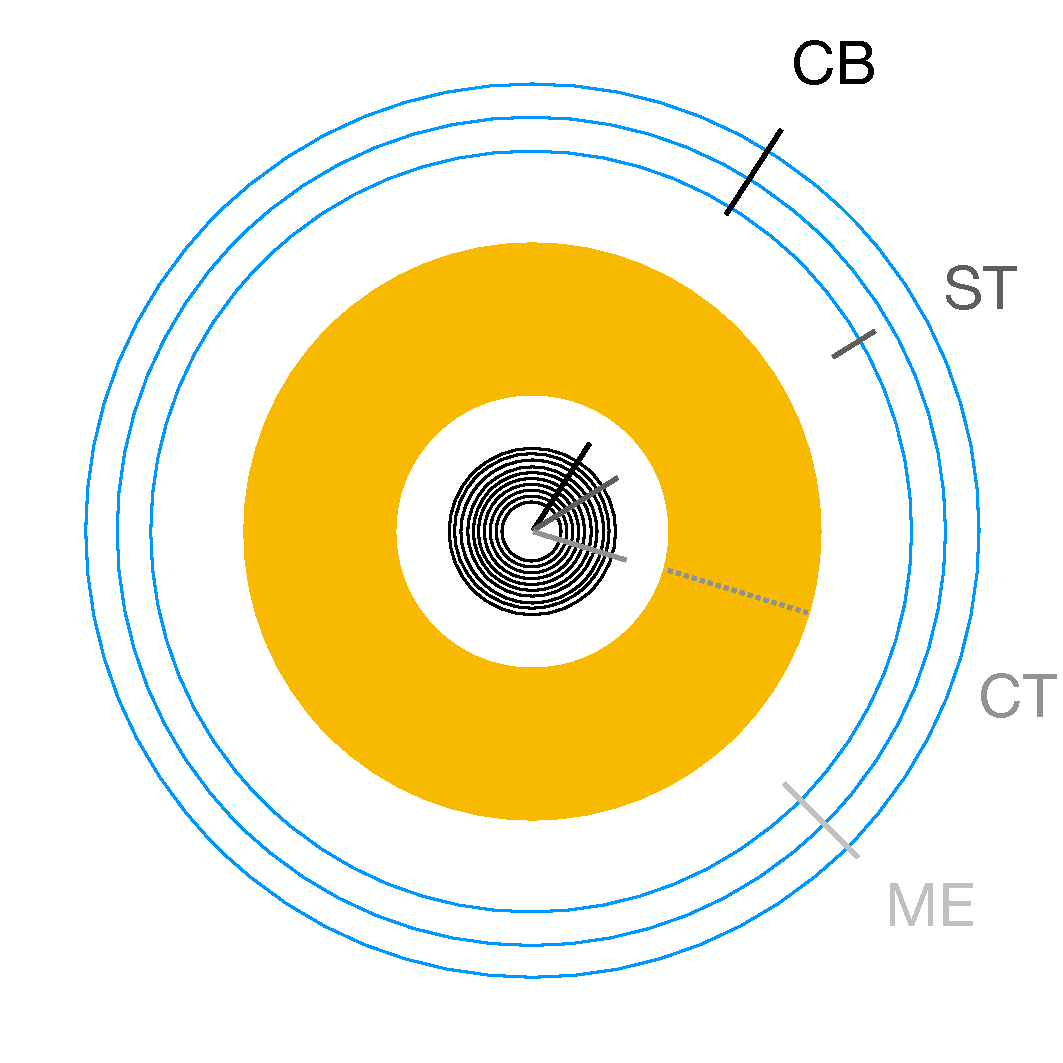
\includegraphics[width=0.5\textwidth]{Figures/LHC/muon_types.pdf}
    \caption{Cross-sectional view of the ATLAS detector and how muon types are identified. The inner black lines represent the inner detector, the yellow is the calorimeter, and the outer blue lines are the muon spectrometer. This figure is adapted from~\cite{Ottersbach:2012mma}.}
    \label{fig:typesofmuons}
\end{figure}
\subsubsection{Muon identification}

Muon identification is carried out with a cut-based approach \cite{ATLAS_muon_reco_2010}. The main backgrounds coming from hadron decays (mostly charged pion and kaon decays) are suppressed by applying quality requirements that select for prompt muons with high efficiency that provide robust momentum measurements. 

There are three identification variables used in discriminating a prompt muon from a background muon. These are:
\begin{itemize}
    \item the q/p significance, $\dfrac{q/p}{\sigma_{q/p}}$, the absolute value of the difference between the muon's charge to momentum ratio as measured in the inner detector and the muon spectrometer, divided by the sum in quadrature of the corresponding uncertainties $\sigma_{q/p}$;
    \item $\rho'=\dfrac{\p_{\text{T}}^{\text{ID}}-\p_{\text{T}}^{\text{MS}}}{\p_{\text{T}}^{\text{CB}}}$, the absolute value of the difference between the transverse momentum measurements in the inner detector and the muon spectrometer, divided by the transverse momentum of the combined track;
    \item the nomalized $\chi^2$ of the fit of the combined track.
\end{itemize}
Together these variables are sensitive in filtering out candidates from charged hadron in-flight decays in the inner detector. These have a topological "kink" that results in a combined track with poor fit quality, and incompatible momentum measurements coming from the inner detector and muon spectrometer. 

Various identification criteria are employed to target the diverse needs of physics analyses. Just like electron identification, the Loose, Medium, and Tight muon identification working points define progressively more restrictive requirements. Unlike the electrons, however, these working points differ not in the thresholds of a likelihood. Rather, they differ in the type of candidate muons permitted and in the requirements on the three variables defined above. 

The Loose muon identification criteria are chosen for the ATLAS work of this thesis, where all four types of reconstructed muons are used. The calorimeter tagged and segment tagged muons are restricted to a smaller region of $|\eta|<0.1$. This working point is designed to maximise reconstruction efficiency all the while providing good-quality tracks \cite{ATLAS_muon_reco_2016}. They were specifically optimised for an ATLAS Higgs analysis in the four-lepton final state \cite{ATLAS_H4l_2015}.  

\subsubsection{Muon isolation}

Just like electrons, muons have additional isolation requirements imposed to reject background, because muons originating from vector boson decays are often isolated while those originating from semileptonic decays are often embedded in jets. The activity around a muon candidate is therefore measured, in a similar manner  to that of the electrons, by summing a cone of transverse momentum and transverse energy in the tracking detector and calorimeter respectively. 

The tracking isolation is $p_{\text{T}}^{\text{varcone30}}$, defined as the scalar transverse momenta sum of tracks with $p_{\text{T}}>1$ GeV in a cone of size $\Delta R=\text{min}\Big(\frac{10}{p_{\text{T}}^{\mu}},0.3\Big)$ around the muon candidate. The contribution from the muon track itself is subtracted. The variability in cone size is to ameliorate performance for high $p_{\text{T}}$ muons \cite{ATLAS_muon_reco_2016}. Likewise, the calorimeter isolation variable, $E_{\text{T}}^{\text{topocone20}}$, is the sum of the topological energy clusters in a $\Delta R=0.2$ cone around the muon, with the energy deposit of the muon and pile-up effects subtracted. Various definitions for the discriminant variables are used to setup different working points. For the four lepton analysis, the FixedCutLoose working point is chosen, with $p_{\text{T}}^{\text{varcone30}}/p_{\text{T}}^{\mu}<0.15$ and $E_{\text{T}}^{\text{topocone20}}/p_{\text{T}}^{\mu}<0.30$. The details of the various muon isolation working points can be found in reference \cite{ATLAS_muon_reco_2016}.

% \cite{ATLAS:2020xtq}


  \chapter{\mFourL: A measurement designed for re-interpretation}
\label{chap:fourlepton}

\chapterquote{Very inspiring quote}
{Very inspiring quote author}

%% m4l motivation
\section{Motivation for the \mFourL measurement}
\label{sec:fourlepmotivation}

The four lepton channel is a particularly interesting channel to study as it receives contributions from many physics processes.  

First and foremost, there is the production of a pair of \PZ-bosons via quark-antiquark interactions in \info[]{s-channel not in SM because it includes neutral ZZZ or ZZ\photon vertex} both the \Ptop- and \Pup-channel. The \Ptop-channel diagram is shown in Figure \ref{fig:m4lfeynman:qqZZ}, and represents, by far, \improvement[]{Read more about why the u-channel diagram is not preferred} the largest contribution to the \ZZ production and thus to the \mFourL distribution. At the low mass end where $\mFourL=m_{PZ}$, there is resonant production of a single \PZ boson via the s-channel diagram in Figure \ref{fig:m4lfeynman:singleZ}. At $\mFourL=\unit{180}{\GeV}$ and beyond, the threshold for the on-shell production of two \PZ bosons is reached and results in a peak in the four lepton invariant mass spectrum. 

Second in magnitude is the gluon-induced production of a \PZ boson pair. This occurs via a triangle or box quark loop, which results in a factor $\alpha_s^2$ suppression. It still plays a substantial role, however, because at small $x$\footnote{Here $x$ is the component of the proton's momentum carried by the struck quark. At the \LHC the protons have very high energies; therefore the \LHC can be described as a small $x$ collider \cite{zotov2012small}} gluon-gluon luminosity is higher than the quark-antiquark luminosity \cite{Glover:194539}. The contribution from this process in on the order of ten percent \cite{Becker:2230817}. Finally in the pool of \PZ boson pairs there is a small contribution from decaying Higgs bosons, which themselves are produced also via gluon fusion, as illustrated in Figure \ref{fig:m4lfeynman:ggHZZ}. There is resonant Higgs production at \mFourL=\unit{125}{\GeV}, and a non-resonant enhancement at $\mFourL=m_{\Ptop}=\unit{350}{\GeV}$ from the top quark loop. Beyond \unit{350}{\GeV}, the Higgs-mediated \PZ boson pair production process destructively interferes with continuum production of on-shell \PZ bosons \cite{Campbell_2016}.

The \mFourL distribution can be a useful probe for certain new physics scenarios. Take for example, the high mass tail of the invariant mass spectrum. This region is dependent on the couplings of the Higgs to incoming and outgoing particles while independent of the Higgs boson width \cite{Campbell_2016}, a unique property that can be exploited to derive model-independent limits on the Higgs couplings, and on the \todo{reword, this is copy pasted} contribution of new states in the Higgs to gluon coupling \cite{Cacciapaglia_2014}. It has also been previously exploited to derive model-independent constraints on the Higgs boson width \cite{Caola_2013}. 

%% Secondly, under specific assumptions a class of models exists for which the off-shell coupling measurement together with a measurement of the on-shell signal strength can be re-interpreted in terms of a bound on the total Higgs boson width. In this paper, we provide a first step towards a classification of the models for which a total width measurement is viable and we discuss examples of BSM models for which the off-shell coupling measurement can be important in either constraining or even discovering new physics in the upcoming LHC runs

\begin{figure}
    \centering
    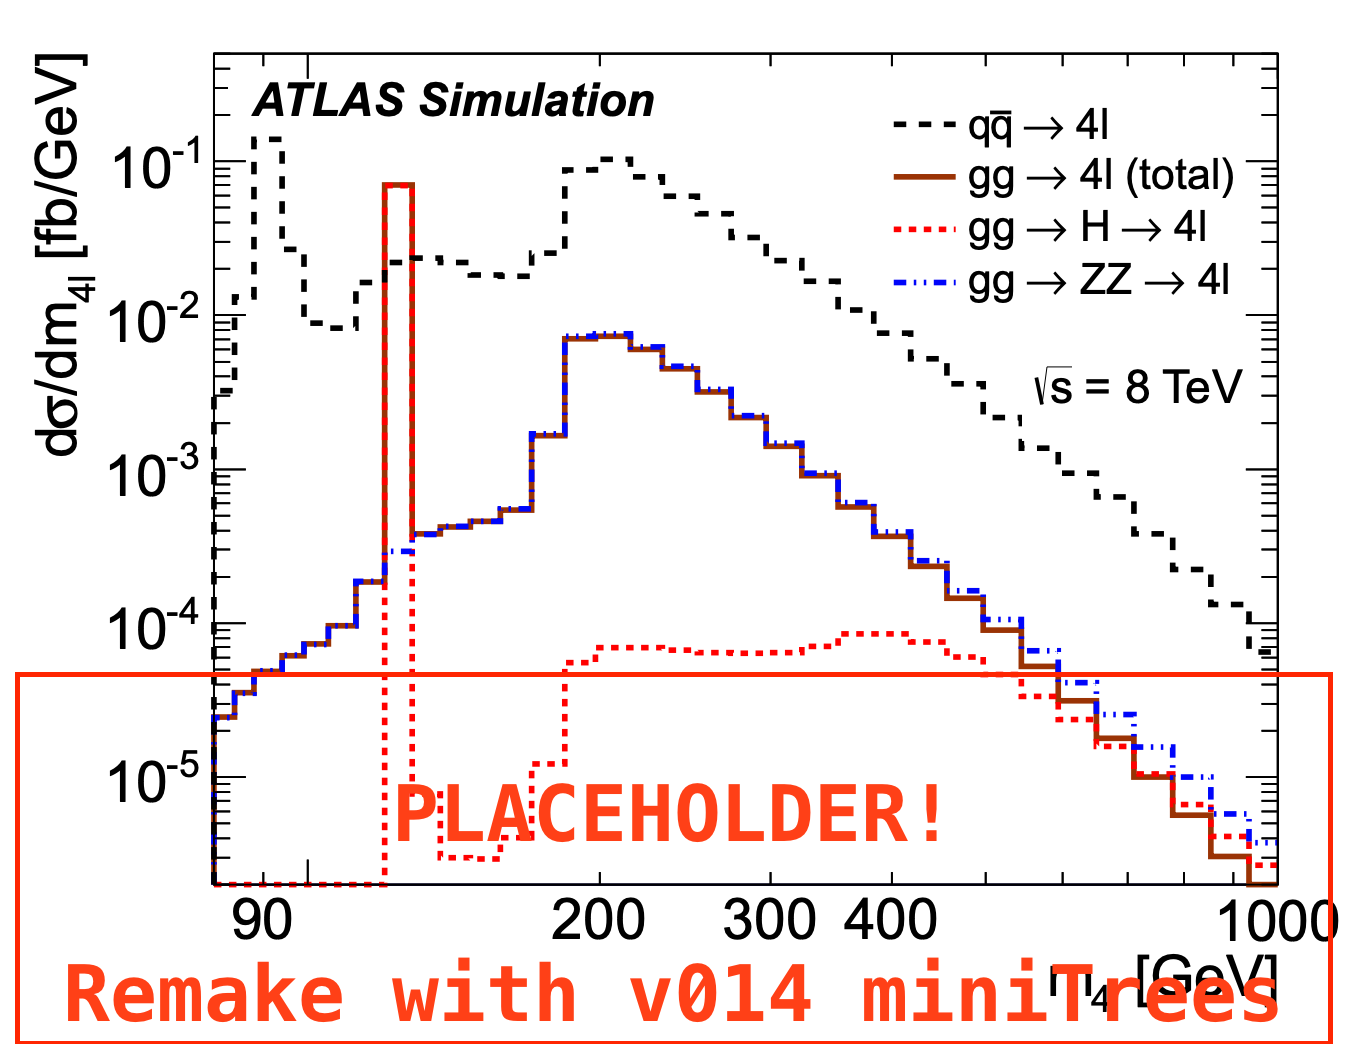
\includegraphics[width=0.5\textwidth]{Figures/m4l/m4lbreakdown.png}
    \caption{Breakdown of contributing processes contributing to the \mFourL distribution.}
    \todo[inline]{Replace and remake with our miniTrees.}
    \label{fig:m4lbreakdown}
\end{figure}

\begin{figure}
\centering
\begin{subfigure}{.24\textwidth}
  \centering
  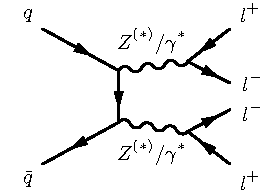
\includegraphics[width=.23\textwidth]{Figures/FeynGraphs/qqZZ4l.pdf}
  \caption{\qqZZ}
  \label{fig:m4lfeynman:qqZZ}
\end{subfigure}%
\begin{subfigure}{.24\textwidth}
  \centering
  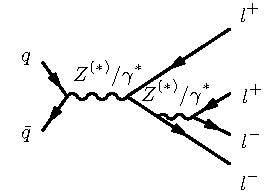
\includegraphics[width=.23\textwidth]{Figures/FeynGraphs/qqZZ4lrad.pdf}
  \caption{A subfigure}
  \label{fig:m4lfeynman:singleZ}
\end{subfigure}
\begin{subfigure}{.24\textwidth}
  \centering
  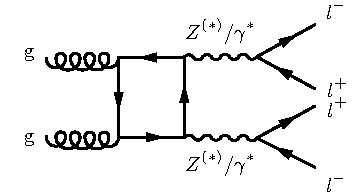
\includegraphics[width=.23\textwidth]{Figures/FeynGraphs/ggZZ4lbox.pdf}
  \caption{A subfigure}
  \label{fig:m4lfeynman:ggZZ}
\end{subfigure}
\begin{subfigure}{.24\textwidth}
  \centering
  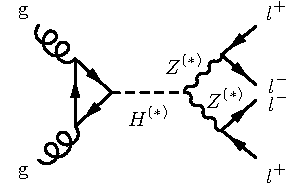
\includegraphics[width=.23\textwidth]{Figures/FeynGraphs/ggZZ4lhiggs.pdf}
  \caption{A subfigure}
  \label{fig:m4lfeynman:ggHZZ}
\end{subfigure}
\caption{Feynman diagrams for quark- and gluon-induced \ZZ production. The processes shown are the main contributors.}
\label{fig:m4lfeynman}
\end{figure}

% this channel provides a clean leptonic final state resulting in a small instrumental background, where one or more of the reconstructed lepton candidates originate from the misidentification of jet fragments or from nonprompt leptons.

%% Signal definition and event selection
\section{Signal and fiducial region definition}
\label{sec:signaldef}

The motivation behind this analysis is to make a measurement as inclusive and as model-independent as possible. Any process leading to a final state of four lepton - made up of two same flavour opposite sign electron or muon pairs - is considered to be part of the signal. Electrons or muons originating from fully leptonic decays of taus are counted towards the signal. 

The fiducial region definition follows closely the acceptance of the detector. Furthermore, by loosening the mass cuts, there is higher event acceptance especially in the low mass regions. Preliminary studies were conducted to investigate the impact of loosening and simplifying the dilepton lower mass cut to \unit{5}{\GeV} and removing the upper mass cut, for example, as opposed to the varying higher cuts in the previous round of the analysis. Unsurprisingly, these result in a higher event yield in both the low and high mass tails of the \mFourL distribution. 

The final state is defined solely in terms of final state particles as opposed to targeting a specific process. Beyond the requirement of two same flavour opposite sign lepton pairs, the measurement is inclusive to additional particles such as additional leptons, jets, and invisible particles. Previous irreducible backgrounds (\VVV, \ttZ) are now considered as part of the signal since they produce four or more prompt leptons.

\missingfigure{Emily plots for loosening mass cuts}

\subsection{Lepton definitions}

For particle physicists, a prompt lepton simply means the lepton did not originate from a hadron. Prompt leptons are further classified into three categories depending on their association with emitted photons. These three categories are:
\begin{itemize}
    \item Born leptons: leptons prior to QED Final State Radiation (FSR);
    \item Bare leptons: leptons after QED FSR;
    \item Dressed leptons: leptons after QED FSR, that then have the four momenta of nearby radiated photons added to it. 
\end{itemize}
The ATLAS detector makes lepton measurements after QED FSR has occurred. It is for this reason that born leptons are not the best choice. It is more realistic to perform measurements involving only final state particles, and objects constructed from final state particles, such as dressed leptons \cite{Kar:ab1be6}. 

\subsubsection{Dressed electrons and bare muons}

In this analysis, a choice of dressing electrons but leaving muons bare was made to closer mimic what is seen by the detector. 

%% Truth isolation
When selecting leptons in the data, there is a complex isolation criteria applied \todo[]{What is this isolation criteria?}. An emulation of this reconstruction-level criteria is included in the fiducial region definition. Although the particle-level application is a simplification, it nevertheless returns a result that is closer to what is actually measured. The particle-level truth isolation criteria requires the sum of the transverse momentum of all charged particles inside a $\Delta R  = 0.3$ cone of the lepton, divided by transverse momentum of the lepton itself, to be less than 0.16. If any other selected leptons are within the cone, their
momenta is not included. 
$$\dfrac{\pt(\Delta R  = 0.3)}{\pt(\text{lepton})}<0.16$$
\subsection{Fiducial region}

\begin{table}[bp]
  \begin{tabular}{lllll}
        & Lepton requirements \\
        \midrule
        Electrons & Dressed lepton definition\\
                & \pt > \unit{5}{\GeV}\\
                & $|\eta| < 2.47$\\
        Muons & Bare lepton definition\\
            & \pt > \unit{7}{\GeV}\\
            & $|\eta| < 2.7$\\
        \bottomrule
        \toprule
        & Event requirements \\
        \midrule
            Four-lepton signature & At least 4 leptons, with 2 Same-Flavour, Opposite-Sign pairs \\
               Lepton kinematics   &   $\pt > 20 / 10$~\GeV{} for
                                     leading two leptons \\ [0.3cm]
              Lepton separation               &   $\Delta R_{ij} > 0.05$ for any leptons \\
              $J/\psi$-Veto &    $  m_{ij} > 5$~\GeV for all SFOS pairs \\
              Truth isolation & ptcone30/\pt < 0.16 \\
  \end{tabular}
  \caption{Fiducial region definition.}
  \label{tab:fidregion}
\end{table}

\missingfigure[]{Dressed electrons, bare muons plot}

\subsection*{Lepton pairing and quadruplet formation} 
\todo[inline]{Reword this whole subsection!!}
Events satisfying the requirements described above enter the fiducial region of the measurement. 
In order to define observables, a unique set of exactly four leptons per event is chosen: 
\begin{itemize}
\item First, the SFOS lepton pair with an invariant mass closest to the Z boson mass is selected as the primary pair in the event. 
\item The remaining SFOS lepton pair closest to the Z boson mass is then referred to as the secondary pair, and completes the quadruplet. 
\end{itemize}
In this way, only one quadruplet is defined even in events containing more than four leptons.
This selection strategy is chosen since it prefers to form pairs that correspond to on-shell Z bosons for the dominant $ZZ$ pair production process, making the pair-level observables based on this definition comparable to such obtained in dedicated $ZZ$ production measurements. This is explored further in Appendix~\ref{app:pairing}. 
The pair and quadruplet formation does not have any impact on the event selection outcome. 

\section{Measured observables}

The star observable of the analysis is none other than the four lepton invariant mass, \mFourL. It has been measured previously by both the \ATLAS and the \CMS experiment \todo{missing citation} \cite{}. As with the previous round of the analysis, the \mFourL distribution is also measured double-differentially, in slices of the transverse momentum of the four lepton system, the absolute rapidity of the four lepton system, and the flavour channel of the four lepton system. 

New to this round of the analysis is the division of the four lepton invariant mass spectrum into four separate regions, each dominated by a different process. From \unit{60}{\GeV}-\unit{100}{\GeV} resonant single \Z production reigns, similarly the \unit{120}{\GeV}-\unit{130}{\GeV} region is dominated by Higgs production, and the high mass region from \unit{180}{\GeV}-\unit{2000}{\GeV} by on-shell \ZZ production. Lastly to fill the gaps between  \unit{20}{\GeV}-\unit{60}{\GeV}, \unit{100}{\GeV}-\unit{120}{\GeV}, and \unit{130}{\GeV}-\unit{180}{\GeV} is the off-shell \ZZ region. This is summarised in Table \ref{tab:m4lregions}. The following variables are measured double differentially in these four regions:

\begin{itemize}
    \item Cosine of angle $\theta^{*}$, where $\theta^{*}$ is the angle between the \todo{definitely check this} lepton in the rest frame and the \Z boson in the lab frame. This angle is sensitive to the polarisation of the decaying boson.
    \item The difference in rapidity between the lepton pairs
    \item The difference in azimuthal angle between the lepton pairs, and between leading leptons
    \item The invariant mass of the lepton pairs
    \item The transverse momentum of the lepton pairs
\end{itemize}

\begin{table}[bp]
  \begin{tabular}{lllll}
        Region & \mFourL interval(s) \\
        \midrule
        \ZFourL & \unit{60}{\GeV} < \mFourL < \unit{100}{\GeV} \\
        \HFourL & \unit{120}{\GeV} < \mFourL < \unit{130}{\GeV} \\
        On-shell \ZZ & \unit{180}{\GeV} < \mFourL < \unit{2000}{\GeV} \\
        Off-shell \ZZ & \unit{20}{\GeV} < \mFourL < \unit{60}{\GeV}, \unit{100}{\GeV} < \mFourL < \unit{120}{\GeV}, \\
          & and \unit{130}{\GeV} < \mFourL < \unit{180}{\GeV}\\
  \end{tabular}
  \caption{The four \mFourL regions dominated by the single \Z, Higgs, on-shell and off-shell \ZZ processes.}
  \label{tab:m4lregions}
\end{table}

\section{Event reconstruction and selection}
\label{sec:eventselection}
A critical aspect of any analysis is its event selection. The dominant backgrounds are shaped by the selection choices, and signal sensitivity are enhanced with optimized cuts. The objective of the selection in this analysis is to efficiently identify the four lepton final states while keeping the background at a minimum. This is achieved through a combination of online trigger (described in detail in Section \ref{ssec:ATLAStrigger}) and offline event selection cuts. As with all \ATLAS analysis, basic requirements on the event cleaning are imposed. Only data recorded with stable beam conditions and with all relevant information from sub-detectors present are considered. 

The requirements on event selection are outlined in Tables \ref{tab:baselineLeptons} and \ref{tab:signalLeptons}. The cuts are largely based on the fiducial region definition of Table~\ref{tab:fidregion} combined with the limited acceptance and efficiency of \ATLAS's object reconstruction. This ensures that there is little to no extrapolation into unmeasured regions on phase space when unfolding. 

First there is the selection of baseline electrons and muons. For both the Loose identification working point is used. For electrons there is a minimum requirement of $p_T>$\unit{7}{\GeV} and $|\eta|>2.7$. For muons it is $p_T>$\unit{5}{\GeV} and $|\eta|>2.47$, and if the muon is a calorimeter-tagged muon there is a more stringent $p_T>$\unit{15}{\GeV} requirement to account for their lower purity. The vertex association requirement ensures that the leptons are associated to the primary vertex in the event. Lastly a lepton-favoured overlap removal is applied to ensure that objects are reconstructed with some distance in between. In the event where a lepton and a jet overlap, priority is given to the lepton. The events that pass these criteria (listed in Table \ref{tab:baselineLeptons}) are classified as baseline leptons.

Additional lepton kinematic requirements are imposed on the leptons after overlap removal. The leading and sub-leading lepton must have a transverse momentum higher than \unit{20}{\GeV} and \unit{10}{\GeV} respectively. The minimum separation between leptons is set at $\Delta R=0.05$ in order to suppress contributions from fake leptons \todo{conversion electrons?}. A $J/\psi$ mass cut at \unit{5}{\GeV} is imposed on all same-flavour-opposite-sign lepton pairs. The $\Upsilon$ contribution is very small, and no mass cut is imposed to suppress it. It is instead subtracted alongside the reducible background from the SM predictions prior to unfolding.

Next, a quadruplet is formed from the baseline leptons containing two same-flavour, opposite-sign (SFOS) lepton pairs. The lepton pair with an invariant mass closest to the \Z mass is the primary pair. Of the remaining leptons, the SFOS pair with an invariant mass closest to the \Z mass is designated as the secondary pair. These are synonymously referred to as the leading and sub-leading lepton pair, respectively. 

The baseline leptons chosen to form the quadruplet undergo a final set of selection cuts outlined in Table~\ref{tab:signalLeptons}. An isolation requirement is imposed to ensure robustness against pile-up. Contributions from other baseline leptons in the vicinity are subtracted from the isolation variables to ensure that the analysis remains sensitive to highly collimated leptons. Background from cosmic-ray muons is suppressed by requiring that a muon's transverse impact parameter $|d_0|<$\unit{1}{\mm}. Each lepton's impact parameter must satisfy a requirement on its significance with respect to the beam line,
\begin{equation}
    \text{S}_{d_0}\equiv\dfrac{d_0}{\sigma_{d_0}}
\end{equation}
where $d_0$ is the transverse impact parameter and $\sigma_{d_0}$ is the associated uncertainty. $\text{S}_{d_0}$ must be smaller than three for muons, and five for electrons. Finally, electrons are subjected to an additional identification criterion requiring a hit in the innermost pixel layer. LooseBLayer is a variation of the Loose working point. 

Like so, the signal region region used in the measurement is defined as the subset of events where all four baseline leptons pass all the signal lepton cuts. Those with baseline lepton(s) that fail the additional cuts of Table \ref{tab:signalLeptons} are not included in the measurement.
 \begin{table}[ht]
    \centering
        \begin{tabular}{lllll}
            Category & Requirement \\
            \hline
            \hline
            Kinematics & Muons : & $p_T > 5$~\GeV{} \\
                       &         &  If CaloTag: $> $15~\GeV \\
                       &         &   $|\eta| < 2.7$  \\[0.2cm]
                       & Electrons: & $p_T > 7$~\GeV \\
                       &            & $|\eta| < 2.47$  \\ 
            \hline
            Vertex association 
                       & Both : & $|z_{0} \sin{\theta}| <$0.5~mm \\
            \hline Identification: 
                       & Muons: & Loose ID  \\ 
                       & Electrons: & LooseLH ID  \\
            \hline
            Overlap removal: Lepton-favoured \\ 
            \hline
            Additional kinematics & Leading lepton & $\pt > 20$~\GeV{}\\
                & Sub-leading lepton & $\pt > 10$~\GeV{}\\
        \end{tabular}
    \caption{Definition of the baseline lepton event selection. \label{tab:baselineLeptons}}
\end{table}  
          
\begin{table}[ht]
    \centering
        \begin{tabular}{l  c }
            Input objects &  Baseline electrons and muons that are part of the quadruplet \\ 
            \hline
            Isolation  &   FixedCutPflowLoose working point\\ %add more detail here/elsewhere
                       &   \textit{Contribution from all other baseline leptons is subtracted} \\
            \hline    
            Cosmic muon veto & Muons: $|d_{0}| < $1~mm\\
            \hline
            Impact Parameter &  Muons: $d_{0}/\sigma_{d_{0}} < $3 \\
                             &  Electrons: $d_{0}/\sigma_{d_{0}} < $5 \\
            \hline
            Stricter Electron ID &  Electrons: LooseBLayerLH ID \\
        \end{tabular}
        \caption{Definition of the signal lepton selection.\label{tab:signalLeptons}}
\end{table}


\begin{table}[ht]
    \centering
        \begin{tabular}{l | c }
            Category & Requirement \\
            \hline
            Event Preselection & Fire at least one lepton \\
                                & trigger \\
                               & $\geq$1 vertex with 2 or more tracks \\[0.2cm]
            \hline
               Four-lepton signature & At least 4 leptons ($e,\mu$)    \\ 
               Lepton kinematics   &   $\pt > 20 / 10$~\GeV{} for
                                     leading two leptons \\[0.2cm]
               Lepton separation               &   $\Delta R_{ij} > 0.05$ for any two leptons \\
              $J/\psi$-Veto &    $  m_{ij} > 5$~\GeV for all SFOS pairs \\
            \hline 
               Trigger matching   & Baseline leptons matched to at least one lepton trigger \\[0.2cm] 
            \hline
              Quadruplet & At least one quadruplet with 2 Same-Flavour, \\
              formation & Opposite-Sign (SFOS) pairs \\
            \hline
              Quadruplet &  4 signal, 0 non-signal: signal region \\
              categorisation    &  $\leq 3$ signal, $\geq 1$ non-signal: background control region \\
        \end{tabular}
        \caption{Definition of the reconstruction-level selection.\label{tab:eventsel}}
\end{table}

 %% Theoretical predictions 
\section{Predictions from Monte Carlo Event Generators}
\subsection{Overview of Monte Carlo Event Generators}
\label{sec:mceg}
Monte Carlo Event Generators (MCEG) play an important role in high energy physics. Generators such as \herwig{}~\cite{Bellm:2017bvx}, \pythia{}~\cite{Sjostrand:2006za} and \SHERPA~\cite{Gleisberg:2008ta} amongst others are essential in data analysis. Together with programs that simulate the detector effects, they are used to estimate the signal and background distributions of various processes. This section gives a brief review of how MCEGs simulate proton-proton collisions, drawing from References~\cite{seymour2013monte,hoche2015introduction,pdg_2021}, to which the readers may refer to for for an in-depth review. 

Protons are composite particles. In order to model how they collide on an event-by-event basis at the LHC, one must model how the partons (valence quarks, sea quarks, and gluons) behave. To achieve this complex goal, the event must be broken up into several phases, each produced via different techniques and occupying a unique region in phase space. QCD is weakly interacting at short distances. Therefore the components of the MCEG dealing with short-distance physics are based on perturbation theory~\cite{pdg}. At larger distances, all soft hadronic phenomena such as hadronization and the formation of the underlying event in hadron collisions cannot be computed from first principles~\cite{pdg}. Instead, one must rely upon other models. This is the general idea behind factorization theorem.

Inside the factorization theorem, an important concept is the Parton Distribution Function (PDF). Written as $f_i(x,\mu_F^2)$, this corresponds to the probability to find a parton of flavour $i$ in the proton as a function of the fraction $x$ of the proton’s momentum carried by the parton and $\mu_F^2$ the energy scale of the hard interaction. $\mu_F^2$ is often referred to as the factorization scale. Since QCD does not predict the parton content of the proton, the shapes of the PDFs are determined by a fit to data from experimental observables in various processes~\cite{placakyte2011parton}.

The event simulation starts at the heart of the collision: the hard scatter. In Figure~\ref{fig:MCEG}, this is the central blob in red. The hard scatter is the one with the largest transfer of energy between the two colliding partons. This is relatively straight-forward to simulate to some fixed order via the matrix element prescription. Nowadays for matrix element calculators, it is standard for most processes to calculate up to Next-to-Leading-Order (NLO), so as to include loop radiative correction. While including higher-order corrections reduces theory uncertainty~\cite{gutschow_lecture}, it is  computationally expensive.

Another important aspect of event generation is the parton shower, which connects the matrix element to the produced and observed hadrons. These are the squiggly branch structures of Figure~\ref{fig:MCEG}. The parton shower describes what happens to the incoming and outgoing parton of the hard collision~\cite{seymour2013monte}. Since partons are coloured, they behave in a Bremsstrahlung-like fashion and radiate gluons as they move through a collision. Recall from Section~\ref{sec:particlecontent} that gluons can also self interact and emit another gluon, leading to an extended shower of partons that is made up of mostly soft gluons~\cite{seymour2013monte}. The parton shower develops with decreasing values of a parameter that is a
measure of the hardness of interactions~\cite{Nagy:98014034}. It is an evolution in momentum transfer scale that starts from the hard process and works to lower momentum until a point is reached where perturbation theory breaks down~\cite{seymour2013monte}. 

As the parton shower branches, the QCD force grows until confinement takes over and results in the partons grouping together into colour-singlet hadrons, illustrated in bright green in Figure~\ref{fig:MCEG}. This process is described using hadronization models. The hadrons simulated may not be stable, meaning that they decay inside the detector volume. The decays are modelled inside the simulations using information about hadron lifetime, branching ratios and hadron decay width~\cite{Cabras:2743914}. Of course, aside from the hard collision there are lots of secondary interactions between the proton remnants~\cite{seymour2013monte}. This is referred to as the underlying event, sketched in purple in Figure~\ref{fig:MCEG}. It produces soft hadrons everywhere in the event, which overlie and contaminate the hard process that was already simulated~\cite{seymour2013monte}.

The MCEGs used to simulate four-lepton events for this analysis, along with key parameters such as PDF set and NLO corrections, are summarized in the next section. The MC samples are used in the design and optimization of the analysis, in evaluating the uncertainties, and in correcting the data from detector inefficiency and resolution effects.
\info[inline]{Simulating the hard process is relatively straightforward because Parton Distribution Functions (PDFs) describe partons coming into the process and lowest order perturbation theory gives a probabilistic distribution of the outgoing partons.}

\begin{figure}[htb!]
    \centering
    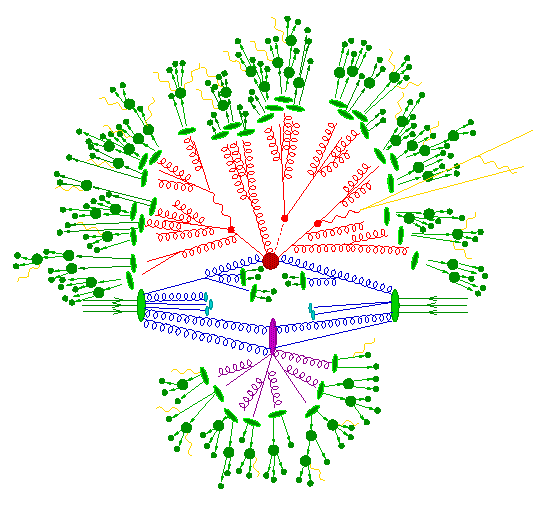
\includegraphics[width=0.90\textwidth]{Figures/LHC/HocheMCEG_final.pdf}
    \caption{This is a diagram of a simulated proton-proton collision. The hard collision is shown in the centre in red. In purple is the secondary hard scattering event. The parton shower is drawn in blue. Hadronisation is sketched in light green, and the subsequent hadron decays and final state particles are shown in dark green. Finally, the electromagnetic radiation is presented in yellow. This figure is from Reference~\cite{hoche2015introduction}.}
    \label{fig:MCEG}
\end{figure}

\subsubsection{Validation of V+jets production in Herwig7 with NLO multi-jet merging}
As part of the \ATLAS author qualification task, multi-leg merging at next-to leading order accuracy using the Matchbox framework in \herwig{7} was explored, with a focus on the vector boson plus jets process. Further details of the task and progression can be found on JIRA (\href{https://its.cern.ch/jira/browse/AGENE-1453}{\code{\textcolor{blue}{AGENE-1453}}}), and in the technical report of~\cite{Huang:2676143}.

\subsection{Monte Carlo samples}
\label{sec:montecarlopred}
This section provides a description of the event samples that are used for this analysis in the standard description of the ATLAS collaboration. These state-of-the-art predictions used to model the signal processes at detector-level and particle-level for this analysis, and to construct the response matrices that correct the data for detector effects. 
\subsection{\qqFourL}
The dominant \qqFourL process is simulated using the \SHERPA {2.2.2} event generator~\cite{Bothmann:2019yzt} with the \nnpdfnnlo{} set of PDFs~\cite{Ball:2014uwa}. The matrix elements are calculated at next-to-leading order accuracy for final states with zero and one jet, and at leading order accuracy for two- and three-jet final states. The different parton multiplicities are merged together and matched to the \SHERPA parton shower model based on the Catani-Seymour dipole factorization~\cite{Gleisberg:2008fv,Schumann:2007mg} using the MEPS@NLO prescription~\cite{Hoeche:2011fd,Catani:2001cc,Hoeche:2009r}. A dedicated set of tuned parton-shower parameters developed by the \SHERPA authors are used. 
An alternate sample of the \qqFourL process is generated using  \POWHEGBOX v2~\cite{Alioli:2010xd,Melia:2011tj,Nason:2013ydw}. The sample is generated at NLO accuracy and interfaced to \PYTHIA 8.186 for the simulation of the parton shower, hadronization, and underlying event. The tuning parameters are set according to the AZNLO tune~\cite{STDM-2012-23}. The sample is corrected to higher order effects using a k-factor obtained with \textsc{Matrix} NNLO QCD prediction~\cite{Cascioli:2014yka,Grazzini:2015hta,Grazzini:2017mhc,Kallweit:2018nyv}. The $K$-factor is defined as the ratio of the NNLO cross-section to the NLO cross-section and applied as a function of \mFourL{}. 
Virtual electroweak NLO effects are accounted for by reweighting both samples with a mass-dependent $K$-factor. The high-order real electroweak contribution of $ZZ$ plus two jets is modelled separately in a \SHERPA{} {2.2.2} sample. 

\subsection{\ggFourL{}}
The gluon-gluon initiated \ggFourL{} process is modelled by \SHERPA{} 2.2.2 at leading order QCD for up to one additional parton emission. The \SHERPA parton shower model based on the Catani-Seymour dipole factorisation is used. Also included in this sample is the s-channel Higgs signal \ggS{} and its interference with the SM box diagram, which has a sizeable contribution above \unit{130}{\GeV}. For particle-level masses below \unit{130}{\GeV} the sample includes on the \ggFourL box diagram because the role of interference is negligible. An NLO QCD $K$-factor is derived using the ratio of the \SHERPA{} sample to an MCFM NLO sample~\cite{Campbell:2011bn}. This is applied as a mass-dependent weight.
An additional constant $K$-factor of 1.2 is applied to account for NNLO effects on the off-shell Higgs production cross-section~\cite{Passarino:2013bha,deFlorian:2016spz}. The sample has a generator cut of $\mll > 10~\GeV$ for same-flavour, opposite-charge lepton pairs. The contribution is below this cut is accounted for through the reweighting to MCFM prediction. Scale and PDF uncertainties are derived in the same way as for the \SHERPA{} \qqFourL{} sample.

\subsection{On-shell Higgs}
The resonant Higgs-boson production is an important process and is generated independently using the most precise description available. The SM Higgs can be produced via gluon-gluon fusion, vector-boson fusion (VBF), Higgstrahlung ($VH$), and in association with a top quark pair ($t\overline{t}H$). The \texttt{PDF4LHC15nnlo} and \texttt{PDF4LHC15nlo} PDF set~\cite{Butterworth:2015oua} are used, alongside AZNLO tune for all on-shell Higgs samples. The dominant gluon–gluon fusion production channel is simulated using the \powheg{} NNLOPS program~\cite{Hamilton:2013fea, Hamilton:2015nsa,Alioli:2010xd,Nason:2004rx,Frixione:2007vw} at NNLO accuracy in QCD, and matched to \pythia~\cite{Sjostrand:2014zea} for the simulation of the parton shower and non-perturbative effects. The sample is normalized to N$^3$LO in QCD cross-sections, which has been calculated for the gluon-fusion process, and corrected for NLO electroweak effects~\cite{deFlorian:2016spz,Anastasiou:2016cez,Anastasiou:2015ema,Dulat:2018rbf,Harlander:2009mq,Harlander:2009bw,Harlander:2009my,Pak:2009dg,Actis:2008ug,Actis:2008ts,Bonetti:2018ukf}. 
\powheg~\cite{Nason:2009ai,Alioli:2010xd,Nason:2004rx,Frixione:2007vw} is interfaced to \pythia{} for the vector-boson fusion process, the $WH$ and $ZH$ production process, and the small contribution from associated productions with a $t\overline{t}$ pair. All are estimated with matrix elements up to NLO in QCD. For VBF, the prediction is reweighted to an approximate-NNLO QCD cross-section with NLO electroweak corrections~\cite{Ciccolini:2007jr,Ciccolini:2007ec,Bolzoni:2010xr}. For VH, the prediction is normalized to an NNLO QCD cross-section calculation with electroweak NLO corrections~\cite{Ciccolini:2003jy,Brein:2003wg,Brein:2011vx,Denner:2014cla,Brein:2012ne}. 
The uncertainties for the on-shell Higgs samples are identical of that of a previous Higgs analysis, the largest of which are from the QCD scale and PDF uncertainties. A detailed description can be found in Reference~\cite{HIGG-2016-22}. 
%  The simulation achieves NNLO accuracy for arbitrary inclusive $gg\to H$ observables by reweighting the Higgs boson rapidity spectrum in \texttt{Hj-MiNLO}~\cite{Hamilton:2012np,Campbell:2012am,Hamilton:2012rf} to that of HNNLO~\cite{Catani:2007vq}.

\subsection{$VVV$ and $t\overline{t}V(V)$}
A smaller contribution to the four-lepton final state originates from triboson processes, and vector-boson production in association of top-quark pairs. These are referred to as $VVV$ (for $WWZ, WZZ$ and $ZZZ$) and $t\overline{t}V(V)$ (for $t\overline{t}Z$ and $t\overline{t}WW$) respectively. The tribon processes are modelled with \SHERPA{} 2.2.2 at NLO accuracy in QCD, with a Catani–Seymour dipole factorization based parton shower provided by \SHERPA{}. Two samples are provided for the  $t\overline{t}V(V)$ contribution. The first is simulated with \SHERPA{} 2.2.0 at LO accuracy up to final states with one additional jet. This sample is used to construct the response matrix used to correct the data for detector effects. The second prediction is produced with the \madgraph~2.3.3~\cite{Alwall:2014hca} generator at NLO accuracy interfaced to \PYTHIAV{8.210}~\cite{Sjostrand:2014zea}. This particle-level predictions of this sample is used to compared against the data for the interpretations of Section \ref{sec:interpretations}. A flat uncertainty of $\pm15\%$ to account for the differences between the two samples is is assigned.

\subsection{Corrections}
All MC events are processed through GEANT4~\cite{Geant4} to simulate the expected response of the ATLAS detector. Next, the samples are passed through the same object reconstruction and identification algorithms as the data and the analysis selection is applied. Pile-up is simulated with \PYTHIAV{8.186} as inclusive inelastic $pp$ collisions. The events are then reweighted to reproduce the distribution of the mean number of interactions per brunch crossing (33.7 on average for the whole dataset). Lastly, events are  reweighted to account for the differences of the lepton reconstruction, identification, isolation, and vertex-matching efficiencies between data and simulation.


 \section{Background estimation}
\label{sec:background}

\subsection{Defining leptons}

The four lepton channel is quite the golden channel, as it has a very clean signature with minimal background. In fact, the single dominant background in this analysis is when one or more of the reconstructed leptons in the quadruplet are not real leptons; rather they are misidentified objects in the detector mimicking the same signature \cite{varnes2016poisson}. These "leptons" are non-prompt, and can be referred to as a fake lepton, whereas a lepton produced from the hard scatter is a prompt, real lepton. One source of fake leptons is from hadron decays. In the case of the electron, photon conversion and hadronic jets misidentified due to their large and narrow deposit in the electromagnetic calorimeter can also play a role. In this analysis, around three-quarters of the fakes originate from \Pbottom-hadron decays in \Z plus jets and \Ptop\APtop events. 

The size and behaviour of the fake lepton background - also referred to as the reducible background - are usually estimated using data-driven methods because they are not well modelled by simulation \cite{varnes2016poisson}. One such method is the Fake Factor method. This method depends on two sets of lepton criteria: a tight criteria that selects leptons which make it into the signal region, and a loose criteria that is similar but less restrictive. The leptons selected by the latter are referred to as baseline leptons, and the baseline leptons that additionally pass the tight criteria are the signal leptons. The rest of this section will also touch on baseline-not-signal leptons; these are leptons that pass the "baseline" loose selection, but do not make the "signal" tight selection. 

\subsection{Fake Factor method}

The Fake Factor method relies on the calculation of a fake efficiency, $f$, which is the fraction of fake baseline leptons pass the tight selection criteria and become signal leptons. Because fake leptons not well modelled in simulation, the fake efficiency is calculated in data, in an alternative region of phase space that is enriched with fake leptons. 

Using the Fake Factor $F$, the number of baseline leptons, and the number of real baseline leptons, the number of fake signal leptons can be calculated. Note that the FF method assumes good modelling in the real component of the simulation since $N^{\text{baseline}}_{\text{real}}$ is taken from MC.
$$N_{\text{fake}}^{\text{signal}} = F(N^{\text{baseline}}-N^{\text{baseline}}_{\text{real}})$$
%% Smoothing
Smoothing on the raw output of the reducible background estimate is performed. The raw output, due to low statistics in certain bins, have pronounced, jagged features that resemble resonances. Of course, resonant peaks should not exist. The smoothing procedure is therefore used to obtain a more even shape, minimizing the impact of any outlier bins that had a large Fake Factor weight. In order to smooth the distribution, an intermediate, finer binning is assigned to each observable and the background estimate is run. The fine-binned intermediate background distribution is smoothed with Friedman's super smoother. Lastly, the final background estimate is obtained by integrating over the smoothed distribution using the coarser, original binning. 

\subsection{Fake background uncertainties}
\label{ssec:fakeuncertainty}

In the fake-factor background estimate, there are five sources of uncertainty considered:
\begin{enumerate}
    \item Dominant in the low- and high-mass tails where \mFourL < 150 GeV and \mFourL > 350 GeV is the statistical uncertainty of the number of events with in the control region. This is propagated through the measurement via the bootstrap method.
    \item The dominant uncertainty in the mid-range region 150 < \mFourL < 350 GeV are the theory uncertainties associated with the subtraction of prompt-leptons in the control region. These come primarily from QCD scale variations in $WZ$ events. 
    \item A smaller contribution comes from the uncertainties in the Monte-Carlo predictions. This covers the modelling of prompt baseline-not-signal leptons, which get subtracted from the background estimation.  
    \item Fourth is the statistical uncertainty in the control region data used for the calculation of the fake factor. This contribution is subdominant. 
    \item Lastly there is a very small uncertainty from the arbitrary choice of number of intermediate bins used in the background smoothing procedure. It is accounted for by comparing the nominal prediction using 500 bins with alternate predictions using 250 or 1000 bins. 
\end{enumerate}

 \section{Measurement uncertainties}
\label{sec:uncertainties}
An important aspect of an experimental measurement is characterizing its uncertainty. Broadly speaking, uncertainties can be divided into two types. The first is the statistical uncertainty, which is caused by inherently unpredictable fluctuations and can be reliably estimated by making repeated measurements~\cite{Kar:ab1be6}. The second is the category of systematic uncertainties, which arise in the estimation of systematic effects such as background, selection bias, scanning efficiency, energy resolution, angle resolution, variation of counter efficiency with beam position and energy, dead time, etc\cite{orear}. Systematic uncertainties are generally more difficult to determine, and cannot be calculated simply from sampling fluctuations \cite{reygers}. The total uncertainty of the measurement is the sum in quadrature of each individual component.

The breakdown and contribution of the uncertainty sources is shown in Figure \ref{fig:m4lsystematics} for the inclusive \mFourL{} spectrum. The dominant is the statistical uncertainty in all but the third mass bin with resonant single $Z$ production, where the lepton efficiencies' uncertainty prevails. Table \ref{tab:SysTablePerSlice} shows the breakdown of the uncertainties on the total fiducial unfolded cross-section, as well as the fiducial cross-section in the four \mFourL{} regions. The data statistical uncertainty plays a dominant role, followed by the uncertainty from the choice of generator. The rest of this section will discuss the different sources of uncertainty and how they are propagated.

\begin{figure}
    \centering
    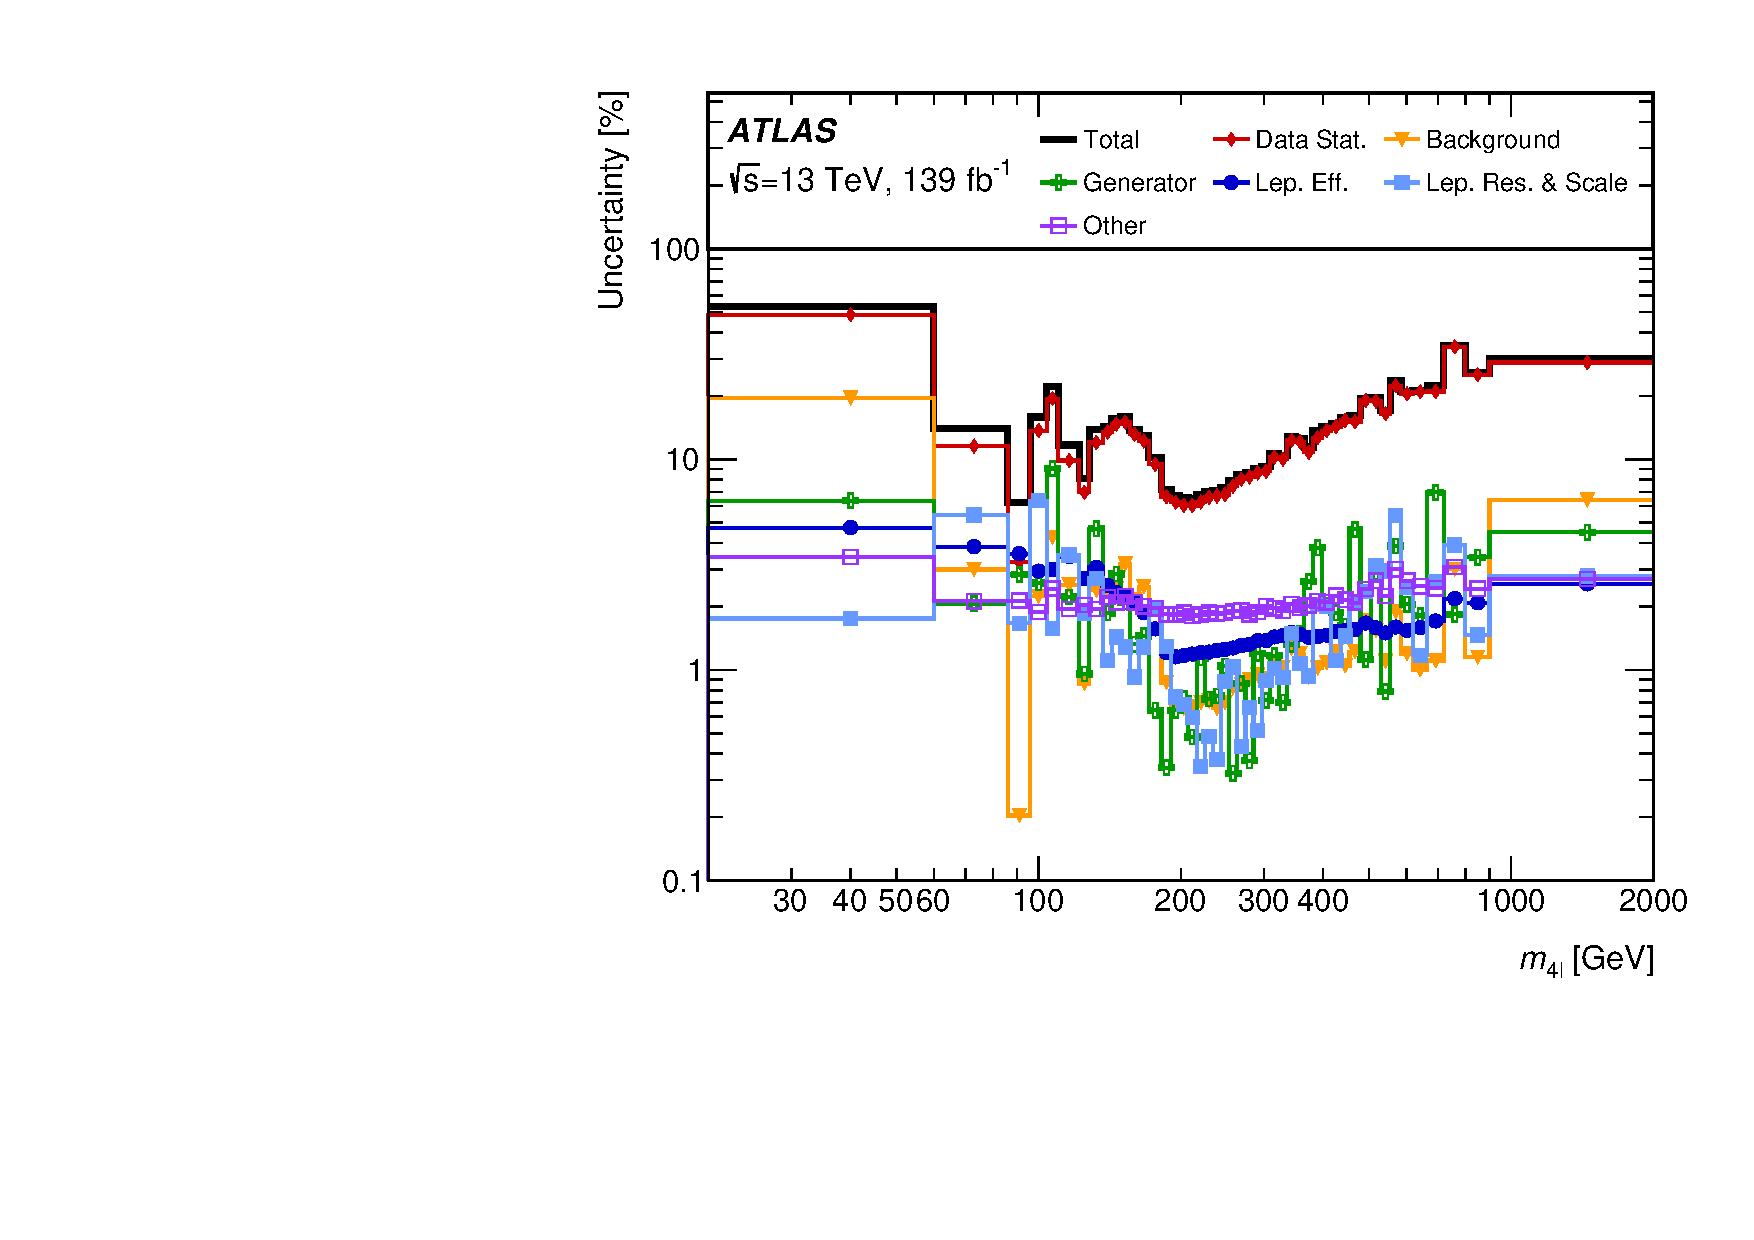
\includegraphics[width=0.85\textwidth]{Figures/m4l/Systematics/UnfoldedSys_M4l_Stack_Paper.pdf}
    \caption{Unfolded systematics for the inclusive \mFourL{} spectrum. The data statistical uncertainty is the dominant source in all but the third bin. This figure is from Ref.~\cite{m4l2021_paper}}
    \label{fig:m4lsystematics}
\end{figure}
\begin{table}
    \centering 
     \begin{tabular} {c  c  c  c  c  c }
         \hline 
         Region  & Inclusive   & $Z\rightarrow 4\ell$   & on-shell $H$   & off-shell $ZZ$   & on-shell $ZZ$   \\
         $m_{4\ell}$ [GeV]  & any   & 60-100   & 120-130   & 20-60/100-120   & 180-2000   \\
            &       &       &       & /130-180 & \\
         \hline 
        DD Closure &  $ 0.088\% $  &  $ 0.35\% $  &  $ 0.13\% $  &  $ 0.45\% $  &  $ 0.035\% $ \\
        Electron ID &  $ 0.94\% $  &  $ \mathbf{1.9}\% $  &  $ \mathbf{1.5}\% $  &  $ \mathbf{1.3}\% $  &  $ 0.49\% $ \\
        Electron Isolation &  $ 0.52\% $  &  $ \mathbf{1.1}\% $  &  $ 0.79\% $  &  $ 0.73\% $  &  $ 0.18\% $ \\
        Electron Reco &  $ 0.84\% $  &  $ \mathbf{1.7}\% $  &  $ \mathbf{1.3}\% $  &  $ \mathbf{1.2}\% $  &  $ 0.31\% $ \\
        Electron Res. \& Scale &  $ 0.46\% $  &  $ \mathbf{1.1}\% $  &  $ 0.83\% $  &  $ 0.54\% $  &  $ 0.12\% $ \\
        Generator &  $ \mathbf{1.3}\% $  &  $ \mathbf{2.6}\% $  &  $ \mathbf{1.3}\% $  &  $ \mathbf{2.7}\% $  &  $ 0.13\% $ \\
        MC Stat. &  $ 0.087\% $  &  $ 0.22\% $  &  $ 0.38\% $  &  $ 0.26\% $  &  $ 0.088\% $ \\
        Muon Isolation &  $ 0.96\% $  &  $ \mathbf{1.6}\% $  &  $ \mathbf{1.2}\% $  &  $ \mathbf{1.2}\% $  &  $ 0.58\% $ \\
        Muon Reco \& ID &  $ 0.83\% $  &  $ \mathbf{1.1}\% $  &  $ 0.91\% $  &  $ 0.89\% $  &  $ 0.82\% $ \\
        Muon Res. \& Scale &  $ 0.3\% $  &  $ 0.65\% $  &  $ 0.55\% $  &  $ 0.53\% $  &  $ 0.13\% $ \\
        Muon TTVA &  $ 0.21\% $  &  $ 0.46\% $  &  $ 0.28\% $  &  $ 0.31\% $  &  $ 0.071\% $ \\
        Non-Generator Theory &  $ 0.27\% $  &  $ 0.31\% $  &  $ 0.23\% $  &  $ 0.45\% $  &  $ 0.27\% $ \\
        Pile-up &  $ 0.73\% $  &  $ \mathbf{1.2}\% $  &  $ \mathbf{1}\% $  &  $ 0.81\% $  &  $ 0.47\% $ \\
        Reducible &  $ 0.8\% $  &  $ 0.55\% $  &  $ \mathbf{1.7}\% $  &  $ \mathbf{2.5}\% $  &  $ 0.74\% $ \\
        Trigger &  $ 0.33\% $  &  $ 0.8\% $  &  $ 0.44\% $  &  $ 0.44\% $  &  $ 0.084\% $ \\
        \hline 
        Total Systematic &  $ 2.6\% $  &  $ 4.8\% $  &  $ 3.7\% $  &  $ 4.6\% $  &  $ 1.5\% $ \\
        Luminosity &  $ \mathbf{1.7}\% $  &  $ \mathbf{1.6}\% $  &  $ \mathbf{1.6}\% $  &  $ \mathbf{1.6}\% $  &  $ \mathbf{1.7}\% $ \\
        Data Stat. &  $ \mathbf{1.3}\% $  &  $ \mathbf{2.9}\% $  &  $ \mathbf{6.2}\% $  &  $ \mathbf{4.1}\% $  &  $ \mathbf{1.5}\% $ \\
        \hline 
        Total &  $ 3.3\% $  &  $ 5.8\% $  &  $ 7.4\% $  &  $ 6.4\% $  &  $ 2.7\% $ \\
        \hline 
     \end{tabular}
    \caption{Uncertainties on the unfolded fiducial cross-section inclusively as well as in the four $\mFourL$ slices studied in this analysis, split by source. Uncertainty contribution larger than $1\%$ are marked in bold to guide the eye. This table is from Ref.~\cite{m4l_internalnote}. \label{tab:SysTablePerSlice} }
\end{table}

\subsection{Statistical uncertainties} \label{ssec:statuncert}

Predominantly, the statistical uncertainty is the dominant uncertainty in most bins of the measured differential and double differential cross-sections. The bootstrap method~\cite{ATLAS_Bootstrap_2021} is used to calculate the statistical uncertainty on the data, and the MC. It is first necessary to construct pseudo-data (also called toys). For each set of pseudo-data, a random value is drawn in each bin following a Poisson distribution where the expectation value is the observed event count that that bin. In total, 3500 pseudo-datasets are generated. Each of these are propagated through the unfolding procedure described in Section \ref{sec:unfolding}. The root mean square of the difference between the unfolded pseudo-data and the unfolded data is taken as the statistical uncertainty in each bin. The statistical uncertainties obtained in this way are equivalent to frequentist confidence intervals in the large-sample limit, while in the bins with few entries, the quoted bands are known to be up to 10\% narrower than a frequentist confidence interval.

The above method of estimating the statistical uncertainty is used as the quoted uncertainty in the measurements. When testing the observed cross-sections against the Standard Model, however, a secondary approach - where the expected number of events is used in place of the observed number of events - is preferred. That is, the 3500 pseudo-datasets follow a Poisson distribution with the mean equal to the predicted reconstruction-level SM event yield. This was motivated by studies in constraining SM effective field theory coefficients where the former approach resulted in unreliable limits. For more details see Section \ref{sec:interpretations}.

\subsection{Systematic uncertainties} \label{ssec:systematics}
Systematic uncertainties arise in nearly every step of the measurement. It is the result of measuring something, or estimating something that is not perfectly known because of certain limitations\cite{barlow2002systematic}. Systematic uncertainties are either experimental or theoretical in nature. The former is common to all analyses and pertains to to the ATLAS detector, while the latter relates to the simulation of physics processes as well as to analysis techniques. 

\subsubsection{Experimental sources}
The flat uncertainty on the integrated luminosity for the for the 2015-2018 datasets of 139 fb$^{-1}$ is $\pm 1.7\%$. The integrated luminosity and uncertainty for the whole Run 2 data-taking period is derived based on a calibration of the luminosity scale using $x-y$ beam-separation scans, following a methodology similar to that detailed in reference \cite{ATLAS-2019-Luminosity}, and using the LUCID-2 detector for the baseline luminosity measurements \cite{Avoni-LUCID-2}. While this uncertainty is not relevant in the unfolding, it applies when converting event counts into a cross-section result as well as during the interpretations.

There is an uncertainty associated with pile-up reweighting, which refers to the reweighting of the Monte Carlo samples in order to reproduce the distribution of the number of $pp$ collisions per bunch crossing ($\mu$) observed in the data \cite{ATLAS_XS_pp}. The uncertainty arises from the modelling of pileup events, including uncertainties in the pp inelastic cross-section. The resulting effects on the measured distributions of this analysis is small.

Lepton identification, reconstruction and isolation, and lepton energy/momentum resolution and scale efficiencies and their uncertainties are derived from data using large samples of $J/\psi\rightarrow\ell\ell$ and $Z\rightarrow\ell\ell$ decays. The uncertainties on the performance are derived following the method reported in reference \cite{ATLAS_muon_reco_2016} for muons and references \cite{ATLAS_electron_efficiency_2015-2017}, \cite{ATLAS_electron_efficiency_2015-2016} for electrons. Typical uncertainties on the identification efficiencies are in the range between 0.5\% to 1.0\% for muons and 1.0\% to 1.3\% for electrons. 

The uncertainty from the non-prompt lepton background estimate has a size-able effect in the low- and high-mass tails of the \mFourL{} distribution, reach up to 11\% and 6.5\% in the first and last bins respectively. The details of the uncertainty estimate on the Fake Factor method is detailed in Section \ref{ssec:fakeuncertainty}.

\subsubsection{Theoretical sources}
The choice of the generator used for the simulation of the \qqFourL{} process in constructing the response matrix for unfolding (see Section \ref{subsec:unfmethod}) is the largest source of theory-related systematic uncertainty. The uncertainty arises from the difference in the modelling of the final-state radiation of photons between the \SHERPA{} prediction and the \POWHEG{} + \pythia{} prediction. To assess the uncertainty, the \POWHEG{} + \pythia{} sample is reweighted to match the \SHERPA{} sample. This is done so no double counting of the unfolding method uncertainty occurs. The data is then unfolded via the standard procedure using the reweighted \POWHEG{} + \pythia{} input. The envelope of the observed ratio between this result and the nominal unfolded result is taken as the generator uncertainty. From the choice of unfolding method, the uncertainty is evaluated using the data-driven closure test detailed in Section \ref{subsec:unfmethod}. 

Other theoretical uncertainties have minimal effect on the unfolding, although their effect is larger on the particle-level predictions that the data is compared against. Generator choice aside, the dominant source is from the factorization and renormalization scale variations, with smaller contributions from PDF uncertainties, parton shower uncertainties, next-to-leading order $k-$factor reweighting uncertainties. Overall, this indicates that a good level of model-independence is achieved.


\section{Detector-level results}
\label{sec:m4lrecoresults}
In this section the detector-level selected events are presented and compared to the SM predictions for the single $Z$, Higgs, \onshellZZ and \offshellZZ mass regions, and for the inclusive \mFourL{} distribution. The reducible background described in Section~\ref{sec:background} is also included. 

The number of selected events in the four \mFourL{} regions over the full fiducial phase space is presented in Table~\ref{tab:RecoYieldTablePerProcess}, along with the predicted number of events, and the predicted background contribution from non-prompt leptons. For the \qqFourL{} process the \SHERPA{} simulation is used. The combined uncertainties (systematic and statistical) are also quoted. The uncertainty in the total prediction takes into account correlations between processes, and therefore contributions in a given column do not trivially add up in quadrature to give the total. Uncertainties in the predictions arise from the sources discussed in Sections~\ref{sec:background} and~\ref{sec:uncertainties}. 

\begin{table}
    \centering    
  \begin{tabular} {l  c  c  c  c  c }
 \hline 
  & \multicolumn{5}{c}{Region} \\
      & Full   & \ZFourL{}  & \HFourL{}  & Off-shell $\Z\Z$  & On-shell $\Z\Z$   \\

 \hline 
\qqFourL{} & $6100 \pm 500$  & $1490 \pm 120$  & $128 \pm 10$  & $800 \pm 60$  & $3640 \pm 280$ \\
\ggFourL{} & $680 \pm 90$  & $10.8 \pm 2.9$  & ~~$3.9 \pm 0.7$  & $49 \pm 6$  & $620 \pm 80$ \\
\HFourL{}  & $245 \pm 20$  & ~~$2.16 \pm 0.18$  & $207 \pm 17$  & $33.5 \pm 3.1$  & $1.98 \pm 0.20$ \\
$VVV$  & $35 \pm 4$  & ~~$0.018 \pm 0.005$  & ~~$0.127 \pm 0.018$  & ~~$2.05 \pm 0.22$  & $32.9 \pm 3.4$ \\
$t\bar{t}$\V(\V) & $123 \pm 19$  & ~~$1.37 \pm 0.22$  & ~~$1.2 \pm 0.2$  & $15.5 \pm 2.4$  & $105 \pm 16$ \\
Background & $330 \pm 50$  & $44 \pm 8$  & $26 \pm 5$  & $129 \pm 19$  & $139 \pm 30$ \\    
\hline 
Total Pred. & $7500 \pm 500$  & $1540 \pm 110$  & $367 \pm 19$  & $1030 \pm 60$~~  & $4530 \pm 290$ \\
\hline 
Data & $7755 $  & $1452 $  & $379 $  & $1095 $  & $4828 $ \\
 \hline 
 \end{tabular}
     \caption{Predicted reconstruction-level yields per process and in total,
      compared with observed data counts, over the full fiducial phase space and in the
      following regions of
      $\mFourL$: \ZFourL{}  ($60 < \mFourL < 100$~\GeV), \HFourL{}  ($120 <
\mFourL < 130$~\GeV), off-shell $\Z\Z$  ($20 <
\mFourL < 60$~\GeV\ or $100 <
\mFourL < 120$~\GeV\ or $130 <
\mFourL < 180$~\GeV) and  on-shell $\Z\Z$ ($180 <
\mFourL < 2000$~\GeV).
     The background row is events with non-prompt leptons,
     including those from $\Z{} + \Upsilon{}$ events.
      The \HFourL{} row includes only the
      on-shell Higgs boson contribution, with off-shell contributions included in
     \ggFourL{}. This table is from Reference~\cite{m4l_internalnote}. \label{tab:RecoYieldTablePerProcess} }
\end{table}

Figure~\ref{fig:recoresults1} shows the inclusive \mFourL{} distribution at the detector level. The data are plotted in black along with the uncertainties. The SM prediction is separated into the individual dominant processes described in Section~\ref{sec:fourlepmotivation} and plotted as stacked histograms. 
Overall the data are in good agreement with the predictions, with some minor fluctuations in the high mass bins due to low statistics. The detector-level plots for the rest of the observables are not shown in the scope of this thesis, but are published in Reference~\cite{m4l2021_paper}. 
\begin{figure}[htb]
\centering
 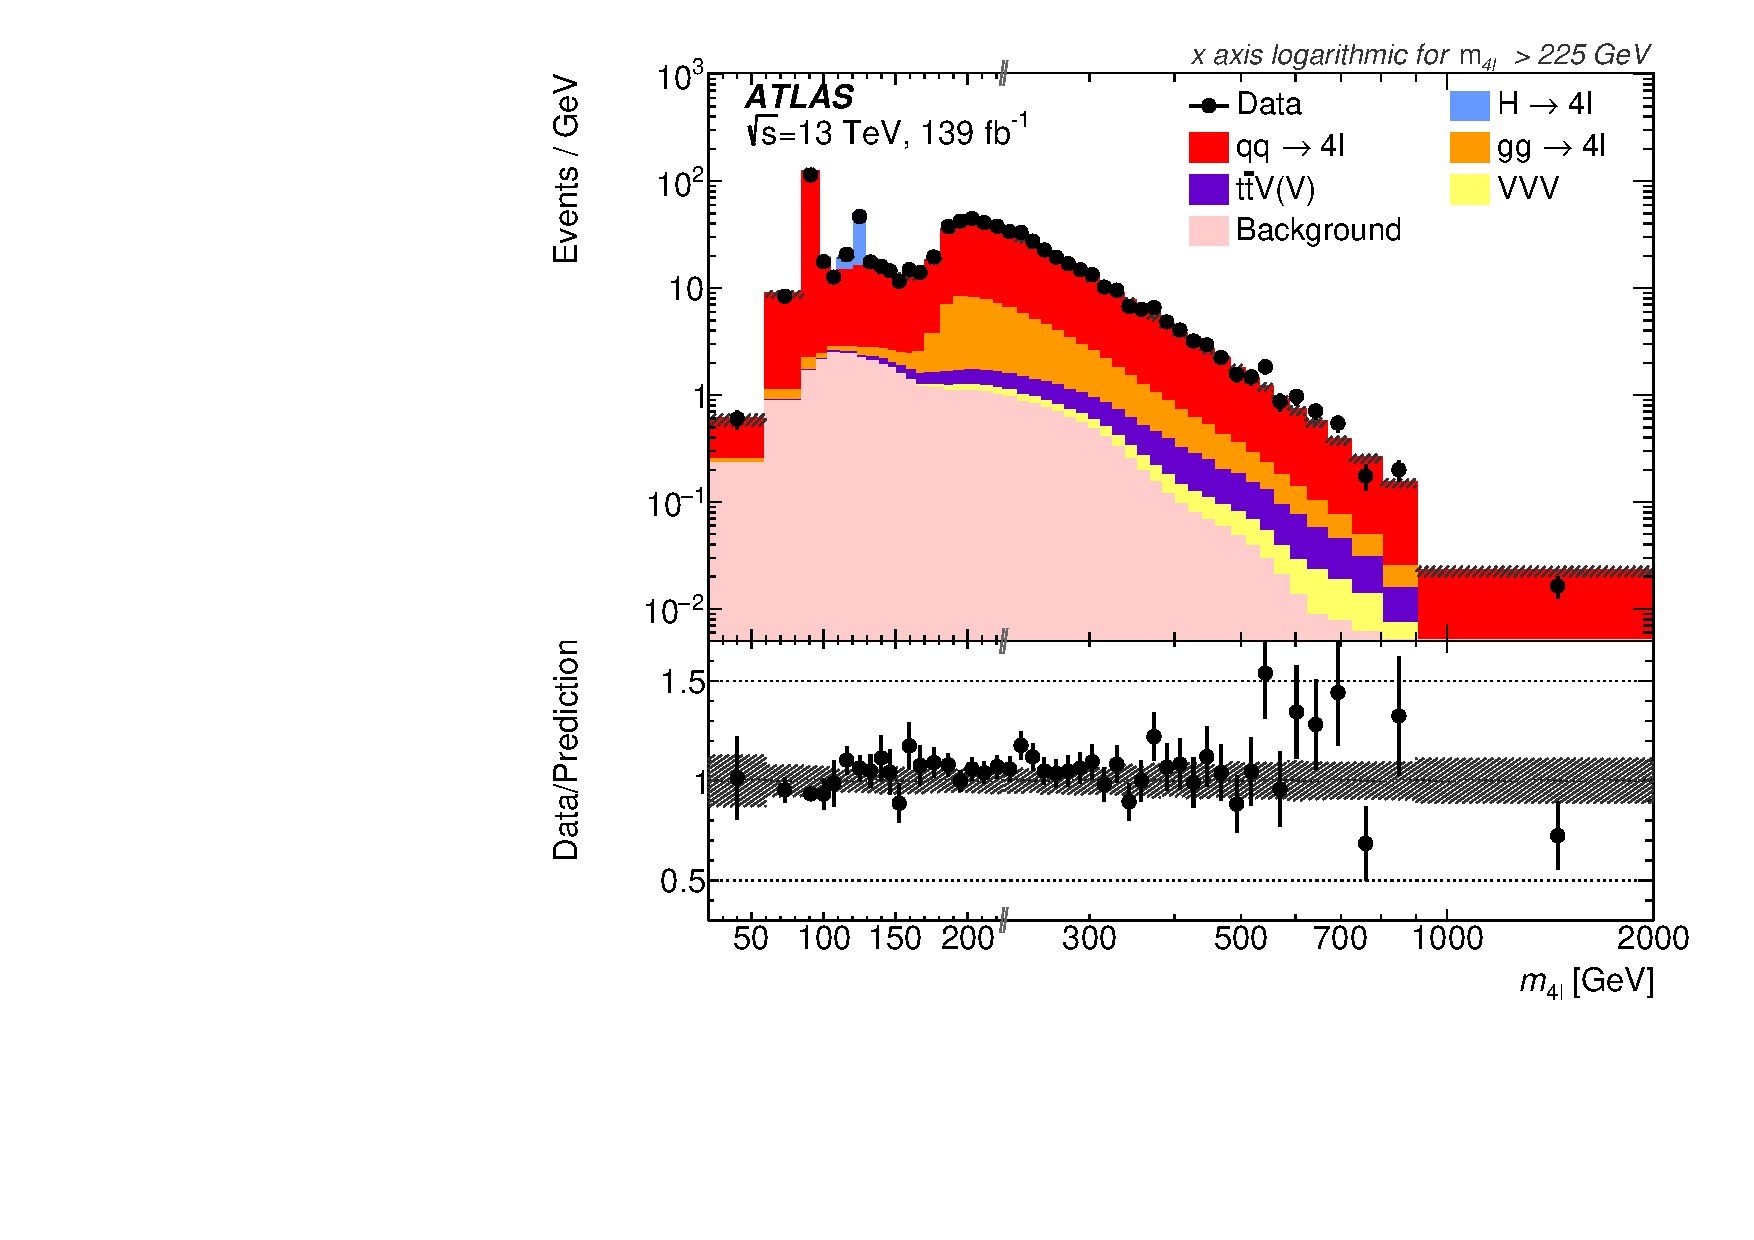
\includegraphics[width = 0.7\textwidth]{Figures/m4l/Overlay_M4l_0__forPaper.pdf}
    \caption{Observed reconstruction-level \mFourL{} distribution compared with the SM prediction, using
      \SHERPA{} for the \qqFourL{} simulation.
     The statistical uncertainty of the
      data is displayed as error bars and systematic uncertainties
      in the prediction are shown as a grey hashed band.  The
      ratio of the data to the prediction is shown in the lower
      panel.  The $x$-axis is on a linear scale until $\mFourL = 225$~\GeV,
where it switches to a logarithmic scale, as indicated by the double
dashes on the axis.
      There is one additional data event reconstructed with 
$\mFourL = 2.14$~\TeV, while 0.4 events are expected from simulation for
$\mFourL > 2$~\TeV. This figure is from Ref.~\cite{m4l2021_paper}. \label{fig:recoresults1}}
\end{figure}

 %% Unfolding and respective studies
\section{Correcting for detector effects}
\label{sec:unfolding}

When an observable is measured by a particle physics experiment, it is important to note that the measured distribution, (i.e. what the particle detector sees) is not what truly occurs at the particle-level. Rather, it is a convolution of the underlying physics process with the effects of the detector. The \ATLAS detector, although an astonishing feat of technology, is still subject to resolution, acceptance, and efficiency limitations. The data at the detector level is smeared and includes the effects of these limitations. For an inclusive measurement such as the four-lepton invariant mass distribution, it is often desirable to correct for these detector effects and present the data at the particle-level. In doing so, the measurement may be directly compared to theoretical predictions, as well as particle-level results from other experiments, in the years to come. In high energy physics, the term coined for this correction procedure is unfolding.

When Unfolding Makes Sense
4
1. Results from experiment A and B with different response function are to be
compared
2. It is too complicated to publish the response function of the detector along
with the data
Detector response might be very complex, e.g., time dependent
Sometimes computer code reflecting the response would have to be published
Danger that future users don't use the filter correctly

\subsection{Unfolding methodology}
\label{subsec:unfmethod}

Unfolding in particle physics can be more generally referred to as a deconvolution. The generic problem statement of deconvolution is to derive a relationship between the true distribution $T(x)$ and the recorded distribution $D(y)$. The two are related by a smearing function $R(x,y)$, which encompasses the instrumentation effects in making the measurement. 
\begin{equation} \label{eq:unfintegral}
    T(x)=\int S(x,y)D(y)dy
\end{equation}
Due to the discretised nature of histograms, the unfolding problem can be stated as a matrix equation:
\begin{equation} \label{eq:unfmatrix}
    x_i=S_{ij}y_j
\end{equation}
where $R$ represents the a smearing matrix of sorts, \todo{add more}$T$ is the true histogram at particle-level, and $D$ is the reconstructed histogram at detector-level. 

For the four-lepton invariant mass analysis, an iterative unfolding method motivated by Bayesian statistics, popularised by Giulio D’Agostini, is chosen. The method iteratively applies the three inputs described above to the measured distributions while using the particle-level SM prediction as a prior.

\subsubsection{An iterative Bayesian approach to unfolding}
\label{ssec:bayesianunfolding}
Let there be a set of causes $C_i$, that can produce one effect $E$. 
\begin{equation}
    P(C_i|E)=\dfrac{P(E|C_i)\cdot P(C_i)}{\Sigma_{k=1}P(E|C_k)\cdot P(C_k)}
\end{equation}

\begin{itemize}
    \item $P(C_i|E)$: given the effect, ithe conditional probability that it was produced from the $i$-th cause.
    \item $P(E|C_i)$: for the $i$-th cause, the conditional probability that the effect is produced.
    \item $P(C_i)$ is the initial probability of the $i$-th cause.
\end{itemize}
If there are multiple possible effects for the causes, then the formula can be generalized to be:
\begin{equation}
    P(C_i|E_j)=\dfrac{P(E_j|C_i)\cdot P(C_i)}{\sum_{k=1}P(E_j|C_k)\cdot P(C_k)}
\end{equation}
The number of expected events for each cause $C_i$ can be obtained by multiplying the number of observations made for effect $j$ with the probability it had been due to cause $i$, and summing over all effects:
\begin{equation} \label{eq:numcause}
    N(C_i)=\sum_jN(E_j)\cdot P(C_i|E_j).
\end{equation}
Here a parallel can be drawn back to equation \ref{eq:unfmatrix}, where $N(C)={N(C_1),N(C_2),...,N(C_n)}$ represents the number of events in the $n$ bins of the true histogram $x_i$, and $P(C_i|E_j)$ corresponds to $R$. Combining these equations, the procedure for estimating the true histogram can be written as:
\begin{equation}
    x_i=\sum_{j=1}^n\dfrac{R_{ij}\cdot P(x_i)}{\sum_{k=1}^nR_{kj}\cdot P(x_k)}y_j.
\end{equation}
Here the matrix defined as $R_{ij}$ is the response matrix. The denominator in the equation is a normalisation factor using the y-projection of the matrix. $P(x_i)$ is the prior, which is updated in each iteration with the unfolded true distribution $x_i$, also known as the posterior.
\todo[inline]{Perhaps mention other unfolding methods and justify choice of this one?}

\subsubsection{Unfolding inputs}

In this analysis the variables of interest are presented as histograms with a finite number of bins. In order to bring these distributions from reconstruction-level to particle-level, there are a number of correction factors to consider:

\begin{itemize}
    \item Fiducial fraction: this is a one-dimensional correction that accounts for events which do not enter into the fiducial region, but pass the detector-level selection nonetheless. These occur due to the finite resolution in the measurement the variables used to select events. The fiducial fraction is defined as the ratio of events that pass both fiducial and detector-level selection to events that pass detector-level selection only.
    \item Reconstruction efficiency: this accounts for the acceptance and efficiency of the detector in reconstructing an event. Of all the events that pass the fiducial selection, only a fraction will be successfully reconstructed and visible to the detector. Formally the reconstruction efficiency is also a one-dimensional correction; defined as the ratio of events which pass both the fiducial and detector-level selection to events that pass fiducial-level selection only.
    \item Migration matrix: each bin in the histogram of the measured observable represents a sub-range of observable values. Sometimes the detector may smear the observable's value high or low enough such that it gets filled to different bins in particle-level and detector-level. These are referred to as bin-to-bin migrations, and is corrected for by the migration matrix. This is constructed as a two-dimensional matrix using events which pass both fiducial and detector-level selection, with the value at particle-level on one axis and the value at detector-level on the other. The matrix, $M_{ij}$, represents the probability that an event which falls into bin $i$ at particle level will fall into bin $j$ when reconstructed at the detector-level. 
\end{itemize}

\subsubsection{Number of Bayesian iterations}

When using the iterative Bayesian method to unfold, the number iterations performed is a key parameter and must be optimised. The method, which uses the nominal MC distribution as an initial prior, results in a bias towards the original shape of the nominal prediction. A way to minimise this effect is to use the obtained unfolded distribution from the previous iteration as the prior for the subsequent unfolding iteration. The more iterations there are, the less dependence there is on the prior, and therefore the smaller the bias. A side effect, however, is that increasing the number of iterations also increases the statistical uncertainty. Fluctuations caused by limited statistics become amplified by the feedback in the algorithm. These effects are thoroughly studied in order to strike a balance between minimising the bias at the cost of increasing the statistical uncertainties.

One thousand toy distributions are generated using the detector-level Standard Model prediction where the value of each bin is randomly drawn from a Gaussian distribution. Each toy is unfolded following the procedure outlined in section \ref{ssec:bayesianunfolding}, where the nominal SM predictions are used to construct the response matrix and for the prior. The bias, written as
\begin{equation} \label{eq:unfbias}
    \text{Bias}_i=\dfrac{\sum_{j=1}^nM_{ij}\cdot x_j-y_i\cdot f_i}{y_i\cdot f_i},
\end{equation}
measures the difference between the product of the migration matrix and the unfolding output, and the product of the detector-level toy and the fiducial fraction. It is an assessment of the strength of the pull that the shape of the SM prior has on the unfolded toy result \todo{Read more about regularisation}. Additional, a statistical uncertainty from the unfolding procedure for each individual toy in each bin is quoted. Next, the bias significance\change[]{italics?} per bin is defined as the quotient of the bias and the statistical uncertainty. After sampling over all toys, the root-mean-square of the bias significance in each bin is calculated. Through the rms bias significance, the size of the bias in comparison to that of the statistical uncertainty is quantified and used as a criterion in determining the number of iterations. The requirement is to use the minimum the number of iterations needed for a bias significant lower than 0.5.

\missingfigure{Optimisation of number of unfolding iterations}

Figure \ref{fig:unfopt} shows the bias, the statistical uncertainty, and the rms bias significance for the inclusive \mFourL distribution. Here the minimum number of iterations for which the criterion is met is three. For the majority of the other measured distributions, three iterations of the unfolding are also found to be optimal. Two iterations are found to be sufficient for the following observables: \mZOne-\mFourL, \dPhill-\mFourL, and \dYPairs-\mFourL.

\subsection{Binning optimisation}
\label{subsec:binningopt}

The binnings of the measured distributions were optimised based on two factors: the number of events and the purity of each bin. Here the purity refers to the diagonal of the migration matrix normalised along truth, thus representing the fraction of truth events that end up in the same reconstructed event bin. There were a few iterations of the binning that were run with varying criteria, summarised in table \ref{tab:BinningVersions}.

The first iteration of the binnings were run with the nominal criteria. Here, depending on the number of events in the bin, the purity requirement varies. Bins with lower statistics have a high purity requirement to reduce bin-to-bin migrations. The minimum number of events required for each bin is 14. Between 14 and 20 events, the purity was required to be at least 80\%. Between 20 and 25 events the purity must be 70\% or higher. Finally for the higher statistics bins with more than 25 events the purity cut was 60\%. 

The binning algorithm is as follows. For the full \mFourL differential mass distribution from \unit{20}{\Gev} - \unit{2000}{\GeV}, the distribution was first split into very fine steps of \unit{1}{\GeV} bins from \unit{20}{\Gev}-\unit{450}{\GeV}. From \unit{450}{\Gev}-\unit{2000}{\GeV} wider steps of \unit{5}{\GeV} bins were used. Due to the fine nature of the bin widths, this initial binning failed to meet any of the binning criteria. Next, the binning algorithm starts from the low mass end and starts to merge adjacent bins together if the criteria were not met. For example, if bin number 1 [20,21] has > 10 events, the algorithm merges bin number 1 with the next bin. The new bin number 1 is now [20,22]. Once again, if this bin has > 10 events, it will merge again and become [20,23], and so on and so forth until 10 events has been reached. Of course the purity must also pass the required percentage for the number of events in the bin, otherwise further bin merging occurs.  

Next we have the \mFourL distributions in double differential slices of \ptFourL, \yFourL, and flavour channel. For these distributions, the fine binning was defined as the the binning of the full \mFourL differential mass distribution, i.e. the output of the algorithm described in the previous paragraph. Bins were once again checked for number events and purity, and merged as needed. This was implemented so that all \mFourL in each of the  \ptFourL, \yFourL, and flavour slices would have bin edges that match with the inclusive distribution. 

For the distributions measured double differentially in the four \mFourL regions corresponding to \Z, \Higgs, On-shell \ZZ, and Off-shell \ZZ, the same procedure was followed for binning optimisation. Each distribution had a fine binning defined, and the bins were merged from left to right of the x-axis until the criteria were met. 

\begin{table}[bp]
  \begin{tabular}{lllll}
                & Nominal              & High statistics             \\
    \midrule
                                & 14 (purity > 0.8) &   \\
     Minimum number of events & 20 (purity > 0.7) & 100    \\
                                &25 (purity > 0.6) &    \\
  \end{tabular}
  \caption{Three different versions of binning with varying criteria.}
  \label{tab:BinningVersions}
\end{table}

\subsection{Pre-unfolding weights}
\label{subsec:preuf}

When correcting the data for detector effects, one of the things to take into account is the efficiency correction. Recall from section \ref{subsec:unfmethod} that the efficiency correction is the fraction of reconstructed events that also pass the fiducial selection cuts. A significant contribution to this is the efficiency correction is efficiency in identifying, reconstructing, isolating, and track-to-vertex-association of (TTVA) leptons. These are dependent on lepton kinematics and calculated from Monte Carlo simulation, therefore they may not be accurate if the data differs from the prediction. To correct for this effect, the lepton efficiencies are measured as a function of the lepton transverse momentum (\pt) and pseudorapidity ($\eta$), and the inverse of this is applied as a per-lepton weight in the data. The term coined for this weight is the pre-unfolding weight, and as the name suggests it is applied prior to the unfolding procedure detailed in \ref{subsec:unfmethod}. 

\begin{figure}
    \begin{subfigure}{.49\textwidth}\centering
        \includegraphics[.99\textwidth]{Figures/m4l/UnfoldingStudies}
    \end{subfigure}
    \caption{Caption}
    \label{fig:my_label}
\end{figure}

Figure \ref{fig:preUF} shows the detector yield from simulation with and without the application of the pre-unfolding weights, compared to the particle yield. It is readily apparent that the detector yield comes much closer to the particle yield when pre-unfolding weights are applied. In some cases, the detector yield surpasses the particle yield around the resonance peaks. This is attributed to bin migrations, and has negligible effects on the final unfolded result. Also shown is the efficiency correction with and without the pre-unfolding weights. In general, a significant increase in efficiency throughout the whole \mFourL spectrum, ranging from 10\% at low mass, up to 25\% at high mass. The conclusion drawn from these plots is that a large portion of the event inefficiency can be accounted for using per-lepton corrections, bringing the reconstructed and particle level yield closer to one another, and minimising the correction needed when unfolding.

\subsection{Unfolding iterations optimization}
\label{ssec:unfoldingiterations}
With the observable binnings defined and the pre-unfolding weights applied, the next step is to optimize the number of iterations used in the unfolding. As described in Section \ref{ssec:bayesianunfolding}, the iterative Bayesian approach to unfolding uses the Standard Model prediction as an initial prior and therefore has a dependence on it. Fewer numbers of iterations therefore correspond to a larger regularizaton bias on the unfolded result. Contrarily, increasing the number of iterations reduces the bias at the cost of a larger statistical uncertainty and results that are more prone to large bin-to-bin fluctuations. The rest of this section describes the metric used to balance these effects and converge on an optimal number of iterations.

First, one thousand toy distributions are generated from the Standard Model predicted yield at the detector level by drawing random Gaussian distributed values for each bin. Under the assumption that the SM accurately describes the underlying physics, each toy distribution represents a possible observation. The toy distributions are unfolded using the nominal unfolding method (Section \ref{subsec:unfmethod}). The bias of the unfolded toy result is defined using the migration matrix $M$, the unfolded yield of the toy $U_{j}$ , detector-level yield of the toy $R_i$, and the fiducial fraction $f_i$ as:
\begin{equation*}
  \text{Bias}_{\text{reco bin }i} = \frac{\sum\limits_{\text{truth bin }j} M_{ij} \times U_{j} - R_{i} \times f_{i} }{R_{i} \times f_{i}},
\end{equation*}
The bias significance of the toy is then be calculated in each bin as the ratio of the bias and the estimated statistical uncertainty of the unfolding procedure. This ratio is a comparison of the sizes of the two effects. 

Next, the bias significance of the one thousand toys are combined into a singular root-mean-square value in each bin. As a result, a metric indicating how significant the bias is expected to be across a range of toy datasets assuming an underlying SM physics is created. The number of iterations is chosen to be the smallest possible while maintaining a root-mean-square bias significance of 0.5 or below. This choice corresponds to a factor two suppresion of the bias compared to the statistical uncertainty. For the majority of distributions, three iterations of the unfolding comfortably satisfy this criteria, whilst for \mZOne-\mFourL, \dPhill-\mFourL and \dYPairs-\mFourL two iterations is sufficient. 
% The bias defined in this way is a measure of to which degree the individual toy is pulled towards the original standard model shape by the regularisation procedure in the unfolding. 
\subsection{Closure tests}
\label{ssec:closuretests}
\subsubsection{Monte Carlo closure tests}

As detailed in Section \ref{subsec:unfmethod}, the unfolding procedure uses a response matrix that has been derived from Standard Model Monte Carlo predictions. A simple test that can be performed to check the validity of the unfolding method is to use the same SM MC prediction at reconstruction level as pseudo-data, unfold it, and compare it to the truth level prediction. This is a self-consistency check, and should yield the trivial result that the unfolded pseudo-data be identical to the truth distribution. This is the full MC closure test, and acts as a sanity check for the unfolding procedure. The test is shown in Figure \ref{fig:fullMCclosure} for the inclusive \mFourL distribution. Full closure is achieved as the unfolded distribution and the particle-level distribution are identical. This is the case for all other distributions as well.

Another similar validation, the half MC closure test, is also performed. This time, the SM samples are divided in two sets A and B based on whether their tagged event number is odd or even. Set A is used to construct the fiducial fraction, reconstruction efficiency, and migration matrix, while set B is used as pseudo-data and unfolded with the inputs from the set A. The unfolded distribution of the set B is then compared to the true distribution of the set B. The statistical uncertainties on both sub-samples are evaluated via the bootstrap method \cite{ATLAS_Bootsrap_2021}. Figure \ref{fig:halfMCclosure} shows the test result for the inclusive \mFourL spectrum. For this and all other distributions, closure is generally achieved within the statistical uncertainties in each bin, with no significant discrepancies. 

\begin{figure}
    \begin{subfigure}{.88\textwidth}\centering
        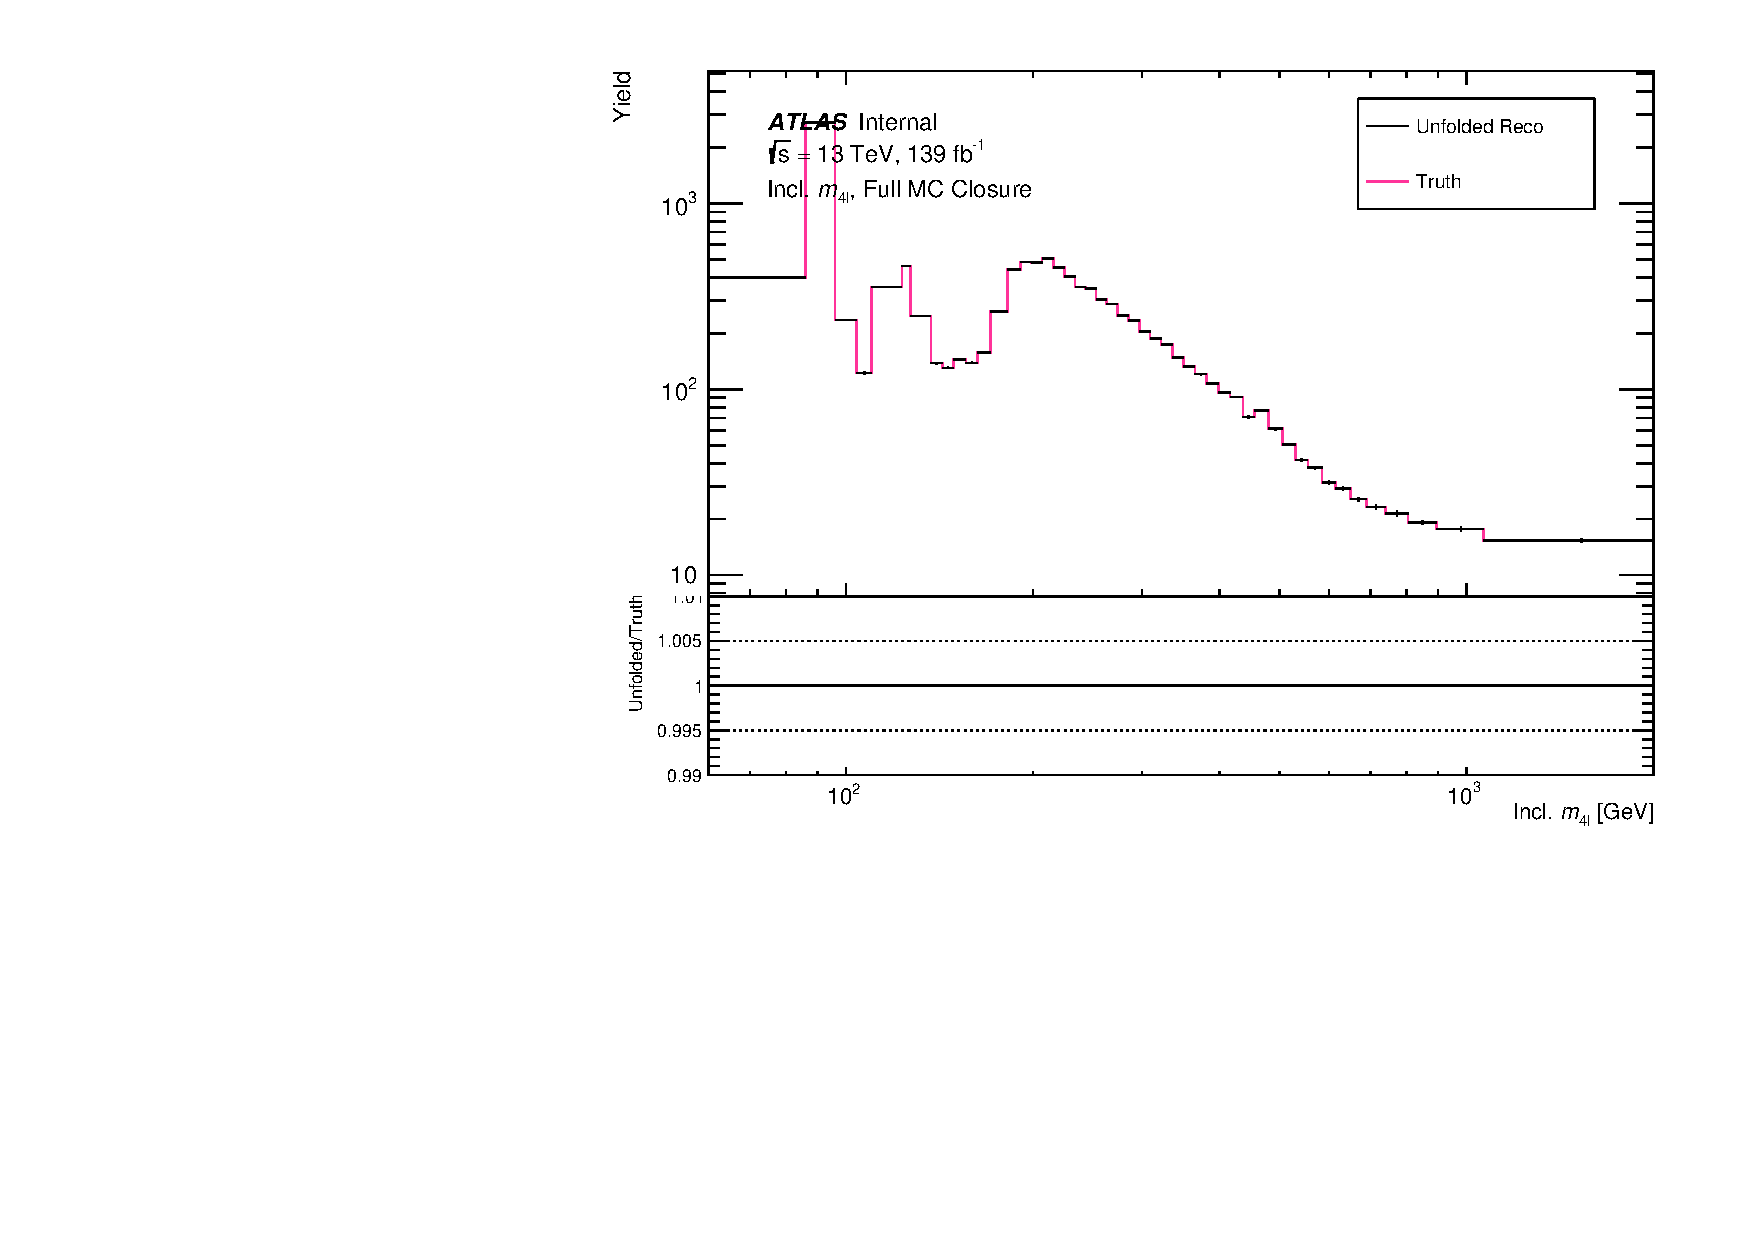
\includegraphics[width=0.90\linewidth]{Figures/m4l/MCClosure/FullMCClosure_inclm4l.pdf}\caption{}\label{fig:fullMCclosure}
    \end{subfigure}
        \begin{subfigure}{.8\textwidth}\centering
        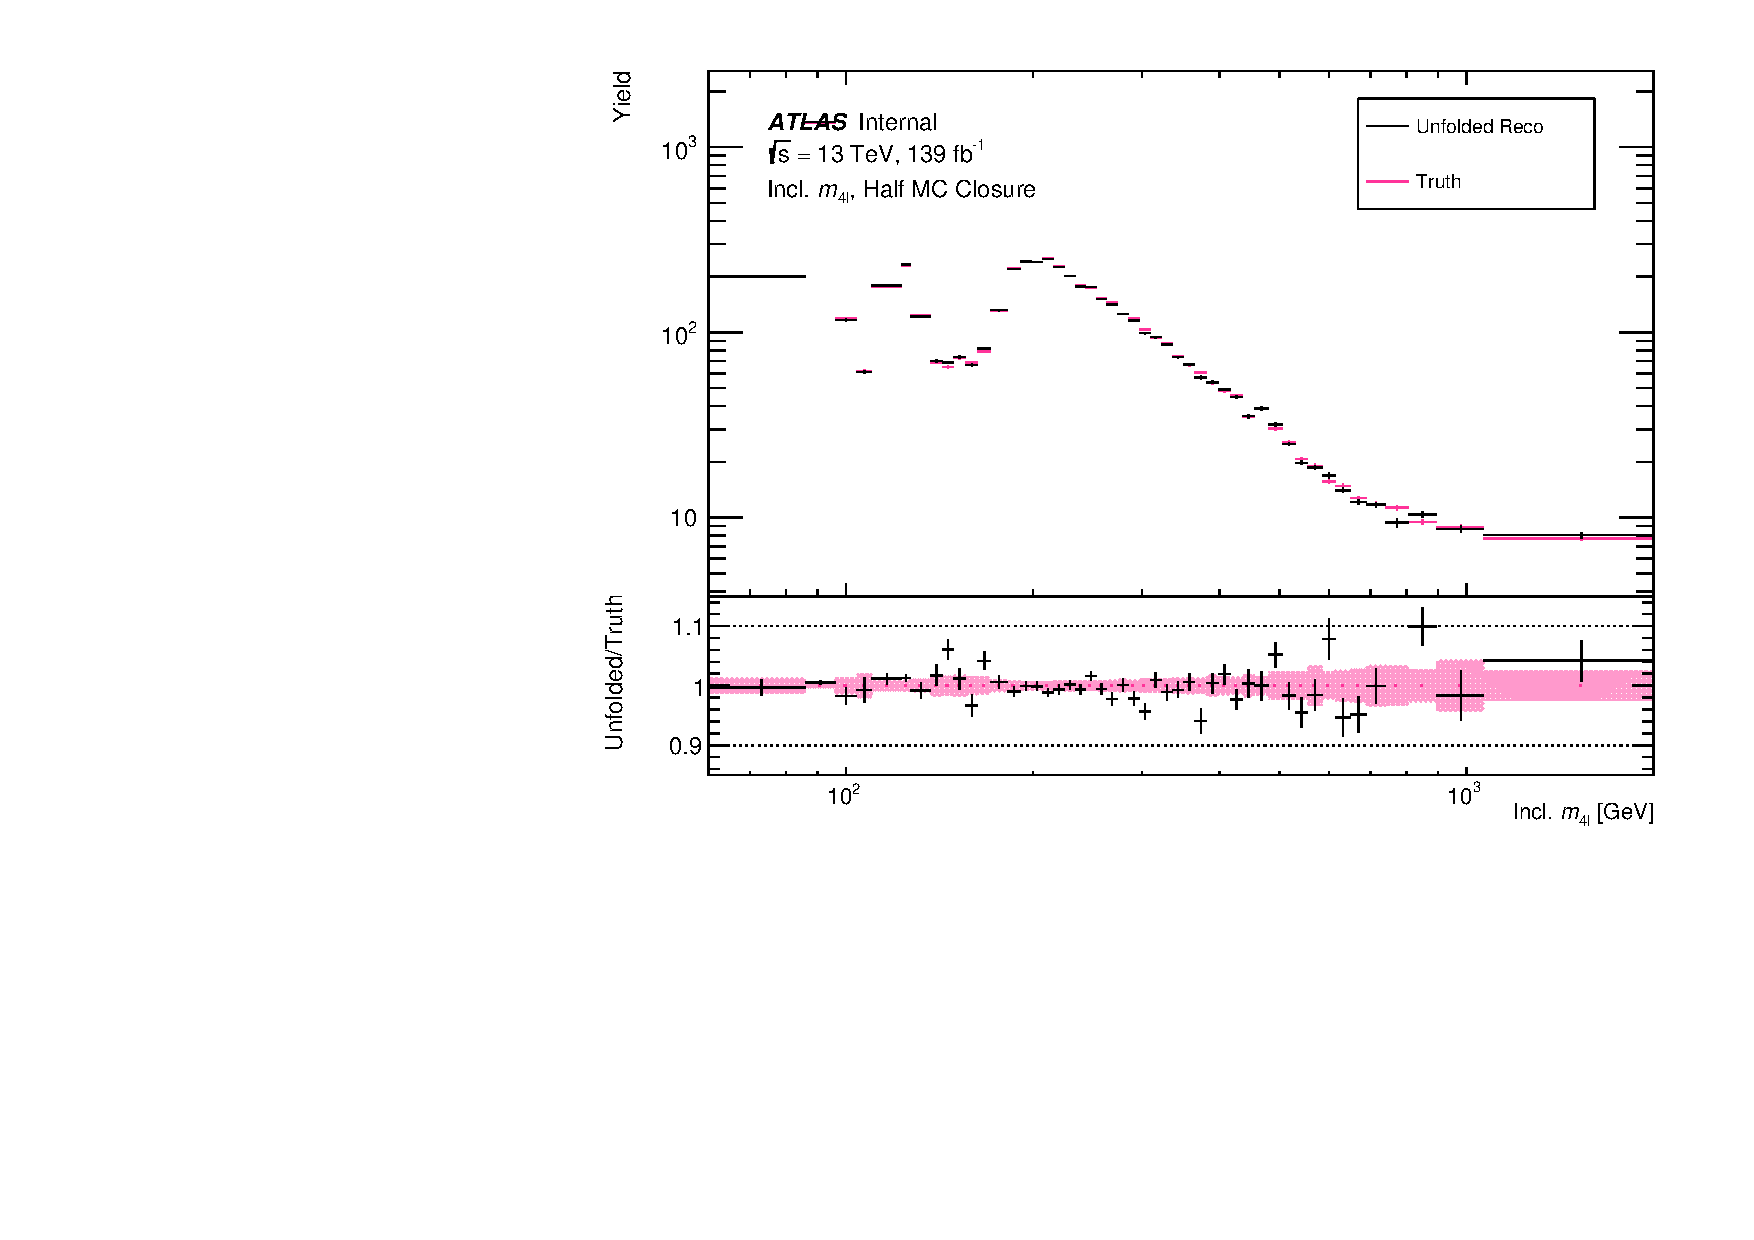
\includegraphics[width=0.99\linewidth]{Figures/m4l/MCClosure/HalfMCClosure_inclm4l.pdf}\caption{}\label{fig:halfMCclosure}
    \end{subfigure}
    \caption{Caption}
    \label{fig:MCclosure}
\end{figure}

\subsubsection{Data-driven closure tests}
\label{sssec:datadrivenclosure}
In order to assess the potential bias in the unfolding method, a data-driven closure test is performed separately for each measured distribution. For this test, a reweighting is conducted on the particle-level MC prediction such that the detector-level prediction represents more accurately the data. The function used for the reweighting is a smoothed function of the data to MC ratio. The reweighted prediction is used as pseudo-data and propagated through the nominal unfolding procedure. The difference between the reweighted particle-level prediction and the unfolded result in each bin is taken to be the systematic uncertainty of the unfolding method. A pictorial description of the process is given in Figure \ref{fig:m4ldatadriven} for the inclusive \mFourL spectrum. The associated systematic uncertainty is below 0.3\% across the full mass range. For the double differential observables, the derived systematic uncertainties averaging much less than 1\% but reaching 3\% in a few bins. Overall, it remains subdominant compared to other sources of uncertainty.
\begin{figure}[htb!]
    \begin{subfigure}{.49\textwidth}\centering
      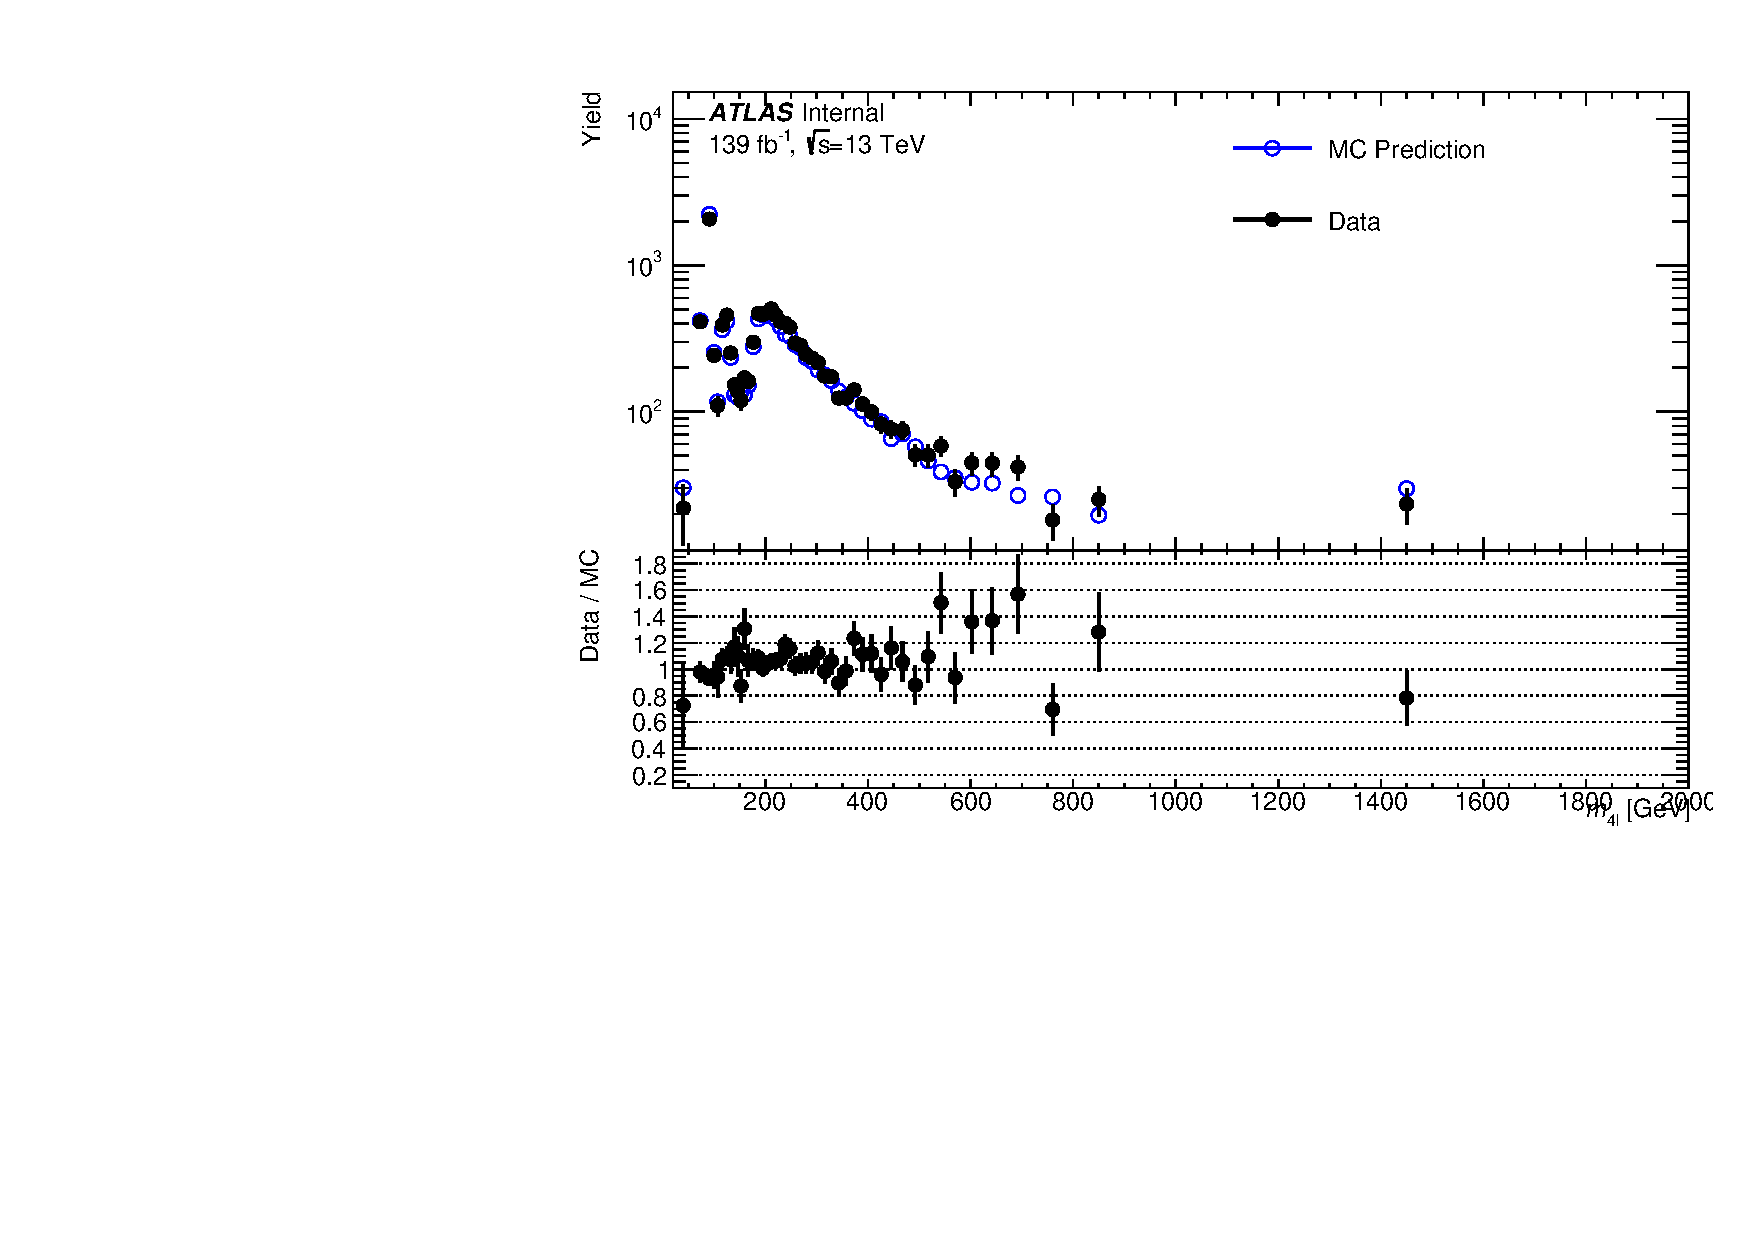
\includegraphics[width=.99\linewidth]{Figures/m4l/DataDriven/RatioM4l.pdf}\caption{}
    \end{subfigure}
    \begin{subfigure}{.49\textwidth}\centering
      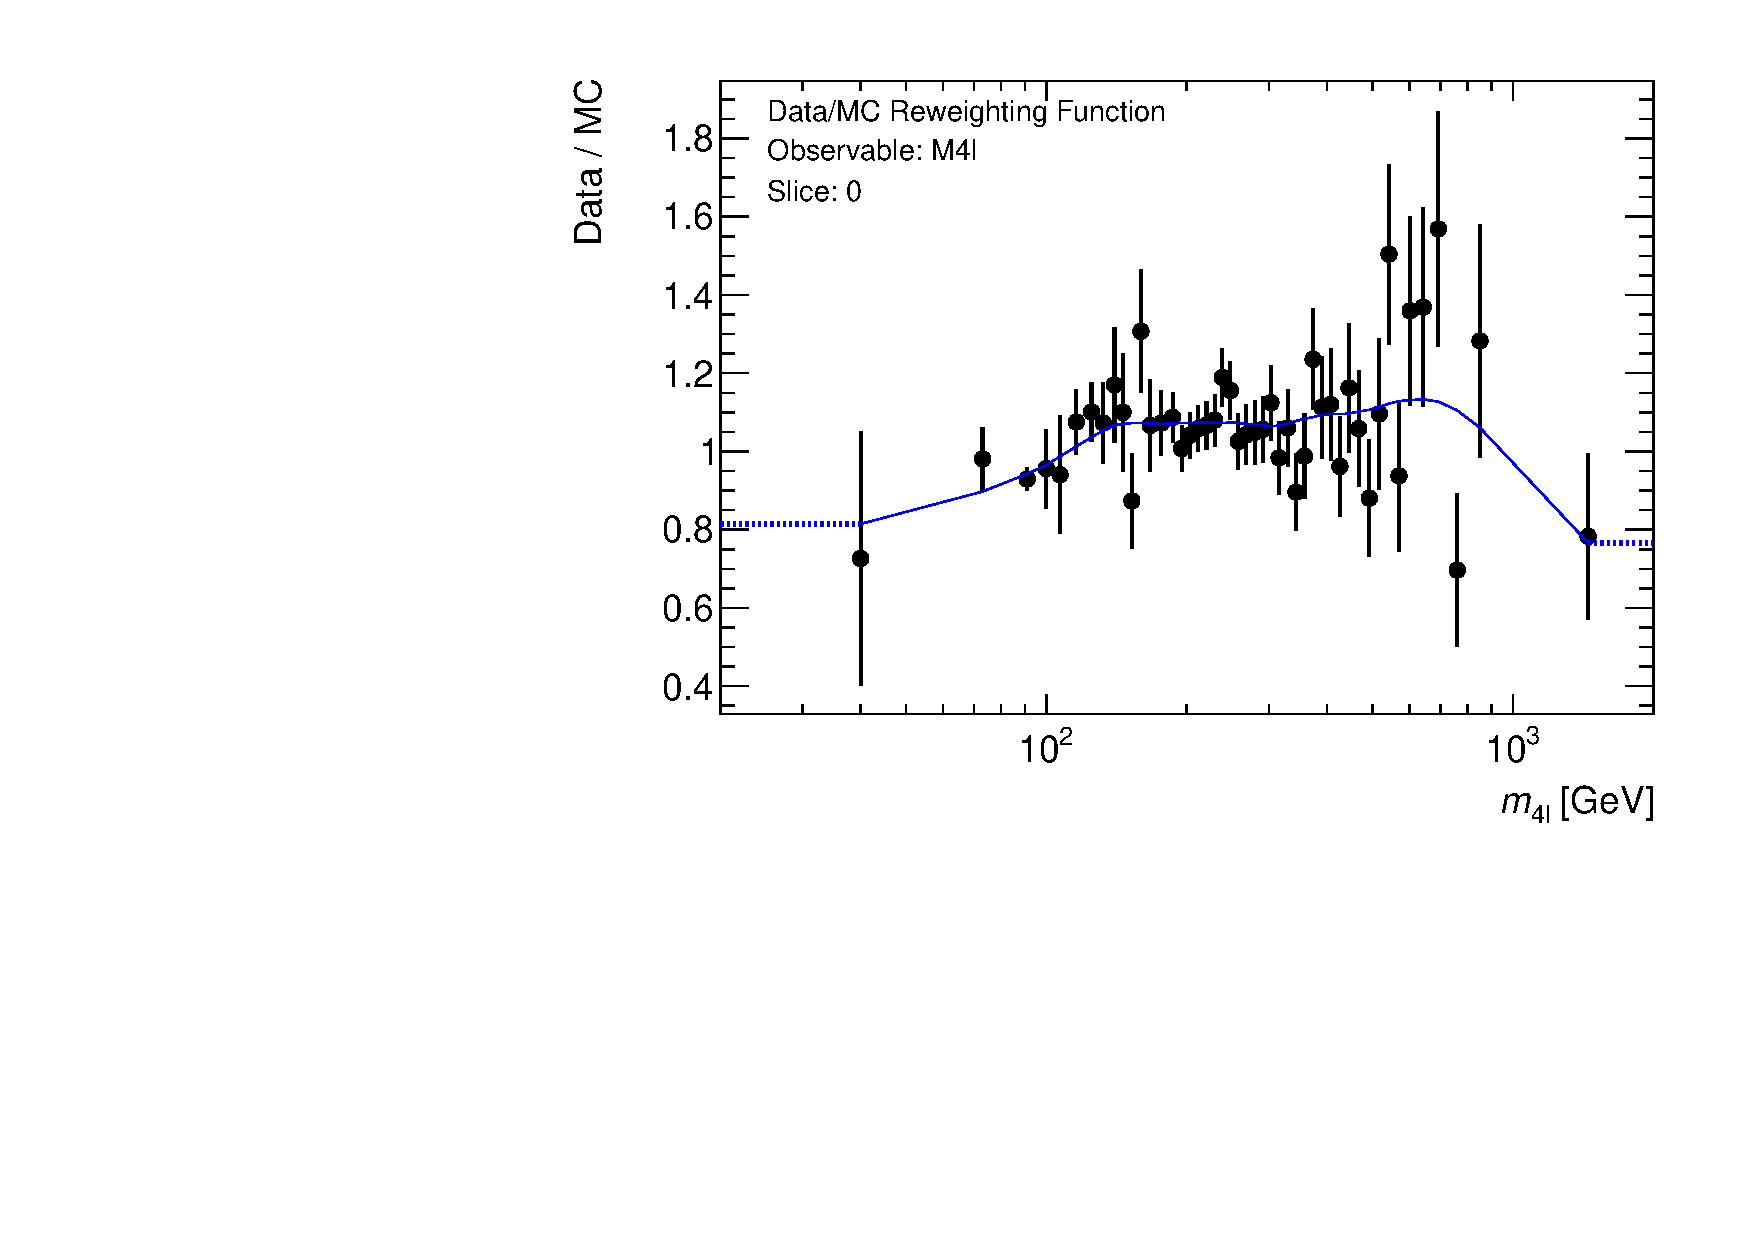
\includegraphics[width=.99\linewidth]{Figures/m4l/DataDriven/FitM4l-Slice0.pdf}\caption{}
    \end{subfigure}
    \begin{subfigure}{.49\textwidth}\centering
      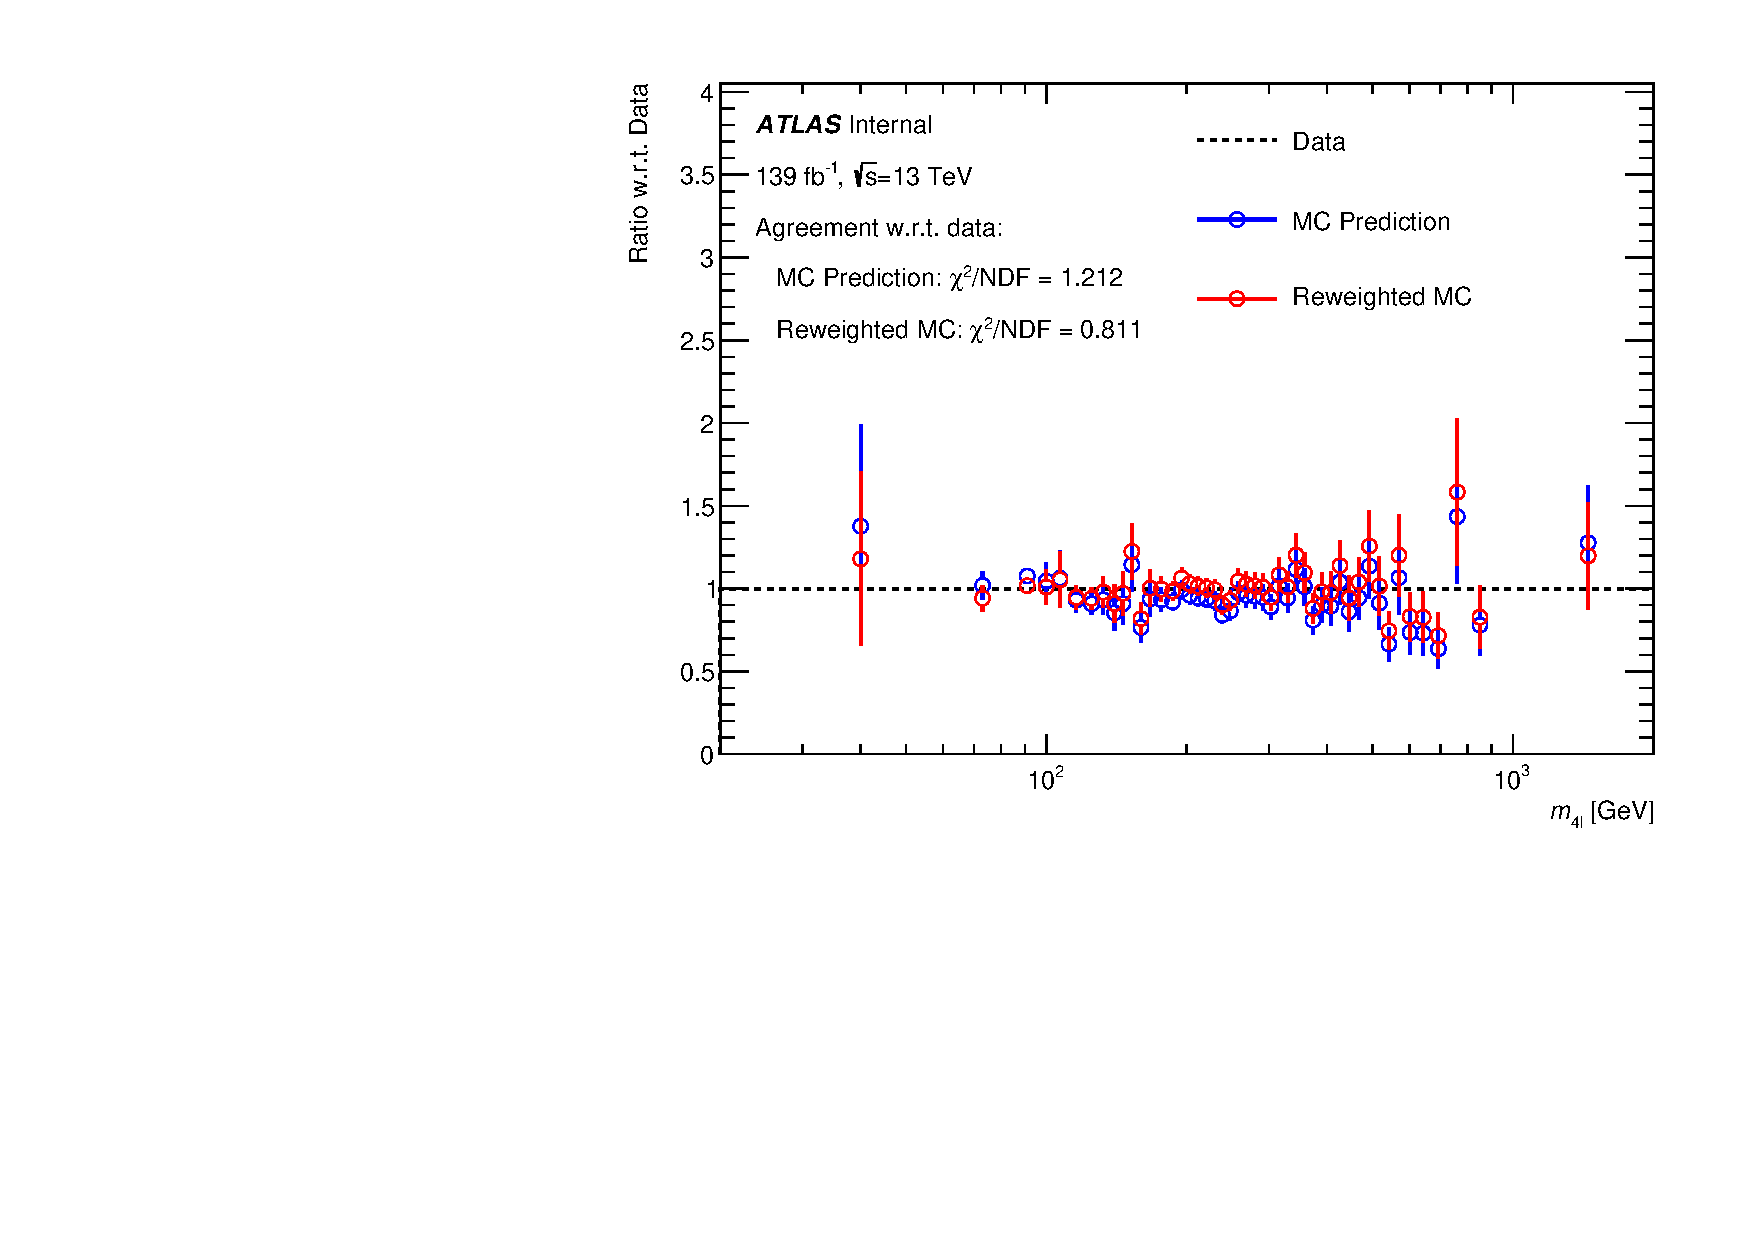
\includegraphics[width=.99\linewidth]{Figures/m4l/DataDriven/ReweightedM4l.pdf} \caption{}
    \end{subfigure}
    \begin{subfigure}{.49\textwidth}\centering
      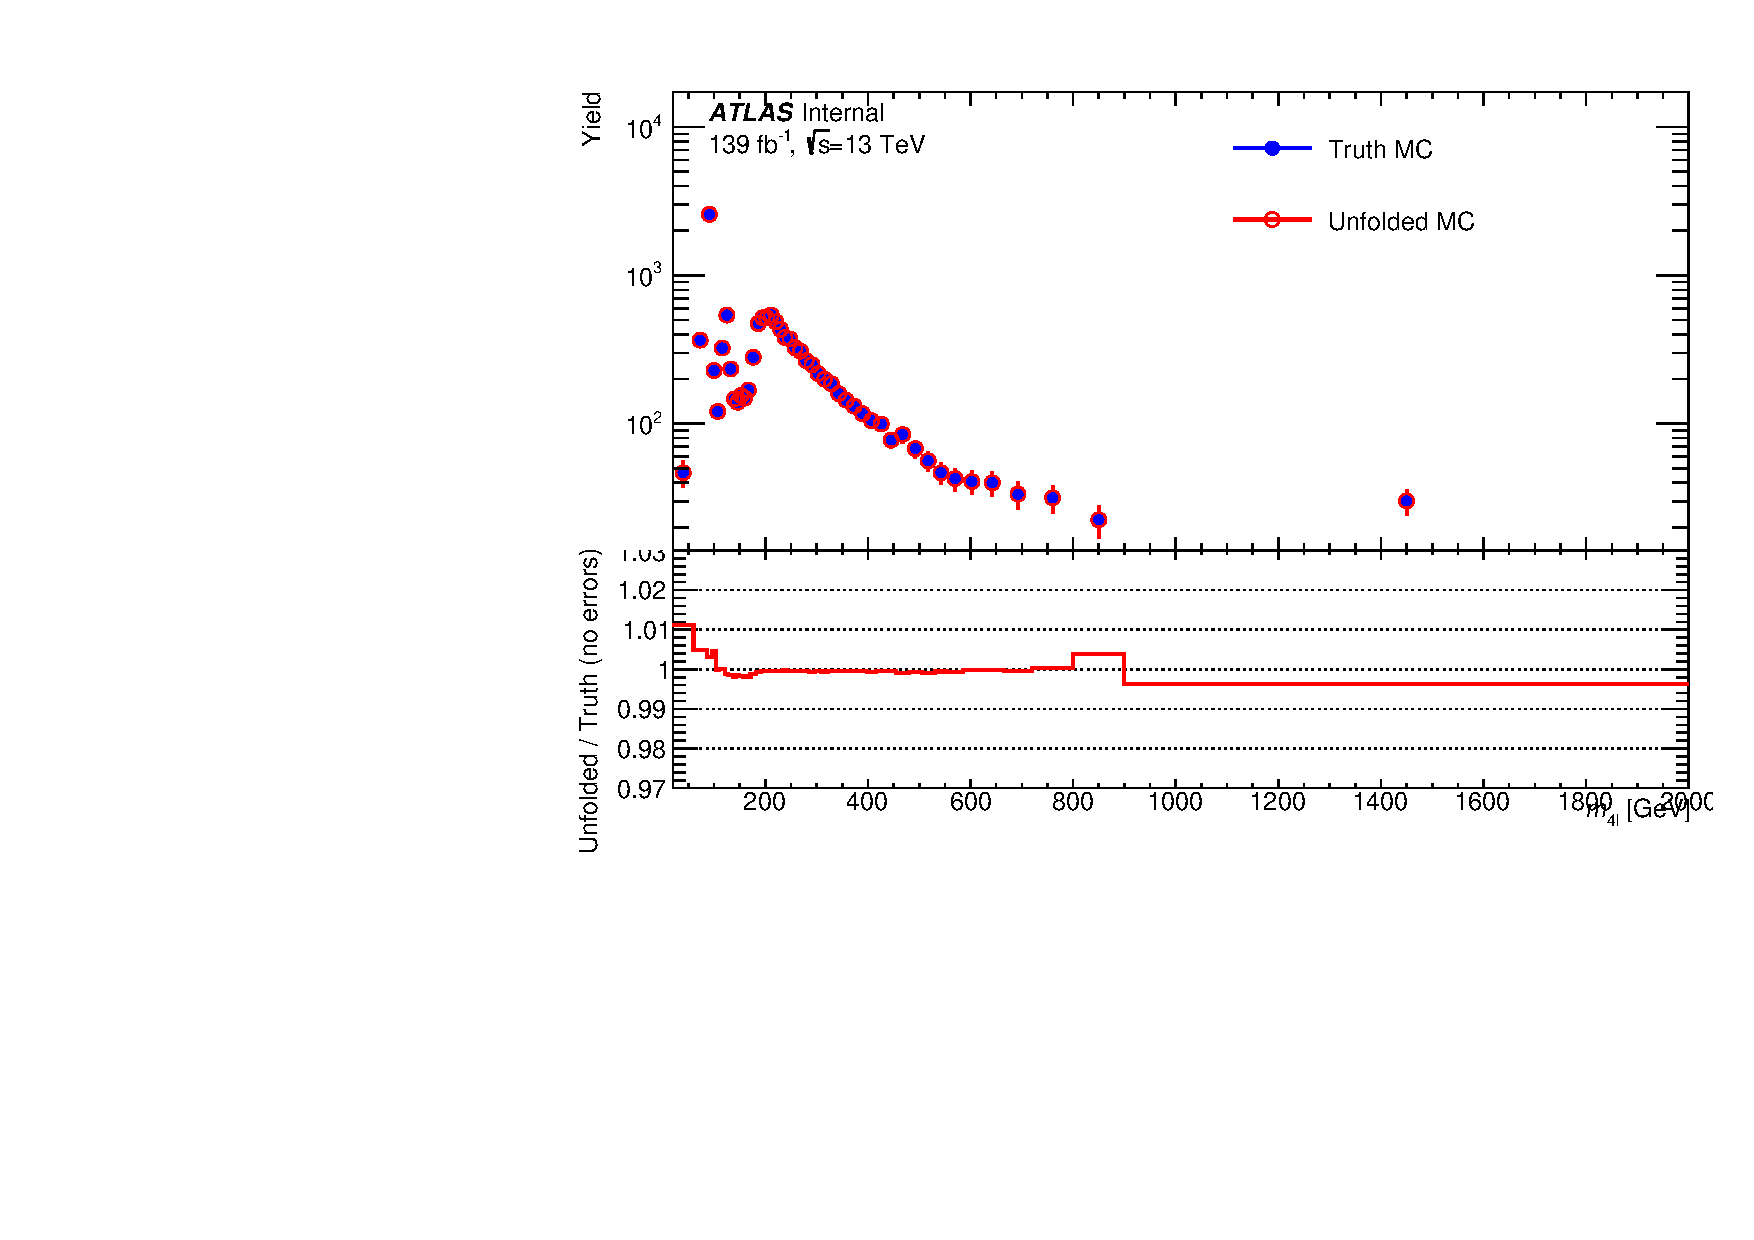
\includegraphics[width=.99\linewidth]{Figures/m4l/DataDriven/UnfoldedM4l.pdf}  \caption{}
    \end{subfigure}
    \caption{Step-by-step overview of the data-driven method for $\mFourL$. In (a), the observed data is compared to the nominal SM MC prediction at reconstruction-level. In (b), the reweighting function is obtained via smoothing of the data/MC ratio and is fixed to its last value in the final bins, as shown by the dashed lines. In (c), the truth-reweighted MC is compared to the nominal MC at reconstruction-level, showing, as expected, an improved agreement with the data. In (d), the difference in the ratio from unity is taken as the relative systematic uncertainty. \label{fig:m4ldatadriven}}
\end{figure}

\subsection{Injection studies}
\label{ssec:injectiontests}
Section \ref{ssec:closuretests} demonstrates that the unfolding procedure has closure when unfolding pseudo-data that agree with the Standard Model. Since the SM predictions themselves were used to derive the corrections and matrix used for unfolding, this is the expected case. The shape of real data is unknown, however, and may be different than the Standard Model prediction. Should the \mFourL spectrum be host to contributions that differ from the SM prediction, it is necessary to check that the unfolding procedure is nonetheless able to provide an accurate and unbiased particle-level result. In order to do this a number of injection tests were performed. The first step is to take the nominal SM prediction, and inject some amount of BSM signal into it. The reconstruction level yield of this modified sample is used as pseudo-data. It is run through the standard unfolding workflow in entirety, and compared to the particle level yield of the modified sample. Conceptually, this procedure is very similar to that of the Monte Carlo closure tests. 

A number of modifications were made to the nominal SM prediction, one set had the addition of a gluon-gluon fusion produced heavy Higgs boson with a mass of 300, 800, or \unit{1400}{\GeV} with either a narrow width or a width 15\% of its mass, and another set where the heavy Higgs was produced via vector-boson fusion. The \ggZZ process was also modified to have a larger event weight with respect to the SM prediction. These are described in full in Table \ref{tab:injectionsamples}. All of the models describe BSM scenarios with extremely large enhancements or resonances. 
\begin{table}[tbp]
    \begin{tabular}{lll}
                            & Injection samples & \\
        \midrule \\
                            &               & 300 GeV \\
         Gluon-gluon fusion &  Narrow width & 800 GeV\\
                            &               & 1400 GeV \\
                            &               & 300 GeV \\
                            & 15\% width    & 800 GeV \\
                            &               & 1400 GeV \\
         \midrule \\
                                & & 300 GeV \\
         Vector-boson fusion    & & 800 GeV \\
                                & & 1400 GeV \\
         \midrule \\
         \ggZZ Enhancement & \\
    \end{tabular}
  \caption{Modifications made to the nominal SM prediction for injection studies.}
  \label{tab:injectionsamples}
\end{table}

For each of the variations listed in Table \ref{tab:injectionsamples}, a range of cross-sections were injected and then unfolded with and without application of the pre-unfolding weights. In order to carve a more realistic scenario, one of the injected cross-sections for the heavy Higgs samples was set to be just within the two-sigma band of the data uncertainty. This was done by increasing the injected cross-section and calculating the $p$-value between the BSM prediction and the data until a $p$-value smaller than or equal to 0.05 is reached. This is the $p$-value corresponding to a two-sigma significance. The results from the injection tests corresponding to a two-sigma injected amount for all the gluon-gluon fusion BSM samples are shown in Figure~\ref{fig:m4l:injection}. The nominal SM prediction and the modified BSM + SM prediction at particle level are shown (SM truth and BSM truth respectively), along with two unfolded BSM distributions, one with pre-unfolding (pre-UF) weights applied and one without. The lower panel is the ratio of the unfolded BSM distribution to the true BSM distribution and is interpreted as the bias. 

Figure~\ref{fig:injection_6dot175fb_300w15} is also published in Reference~\cite{m4l2021_paper}. It shows the result of the injection test using a BSM model with a resonance mass of $m_{\mathrm{res}}=300~\GeV{}$ and width 15\% of the mass, with a cross-section of \unit{6.18}{\invfb}. Looking at the ratio panel, the bias goes up to 2.2\% without the application of the pre-unfolding weights (in green). With the weights applied, the bias is smaller and remains within a $\pm0.8\%$ range (in black). The same trend holds true for the rest of the 15\% width samples, see Figures~\ref{fig:injection_0dot862fb_800w15}-\ref{injection_0dot4032fb_1400w15}. Application of the pre-unfolding weights tend to result in a smaller bias, especially for 300~\GeV and 800~\GeV resonances. For the highest resonance mass at 1400~\GeV, the pre-unfolding has a notable effect only in the last \mFourL mass bin, where it reduces the bias from 10\% to 4\%.

The gluon-gluon fusion narrow-width heavy Higgs models' injection test results are presented in Figures~\ref{fig:injection_1dot24fb_300NW}-\ref{fig:injection_0dot19fb_1400NW}. The unfolding method is much more sensitive to, and therefore less robust to, the presence of narrow resonances. Here, the pre-unfolding is not as effective in mitigating the effects of the BSM signal. The differences between the unfolded BSM and the truth BSM, however, is still within 6\% bias for the 300~\GeV and 1400~\GeV resonance mass models. For the 800~\GeV model this goes up to 16\%. In all cases, the bias is well within the total uncertainty in the corresponding \mFourL mass bin. 

\begin{figure}[htb]
    \begin{subfigure}{.49\textwidth}\centering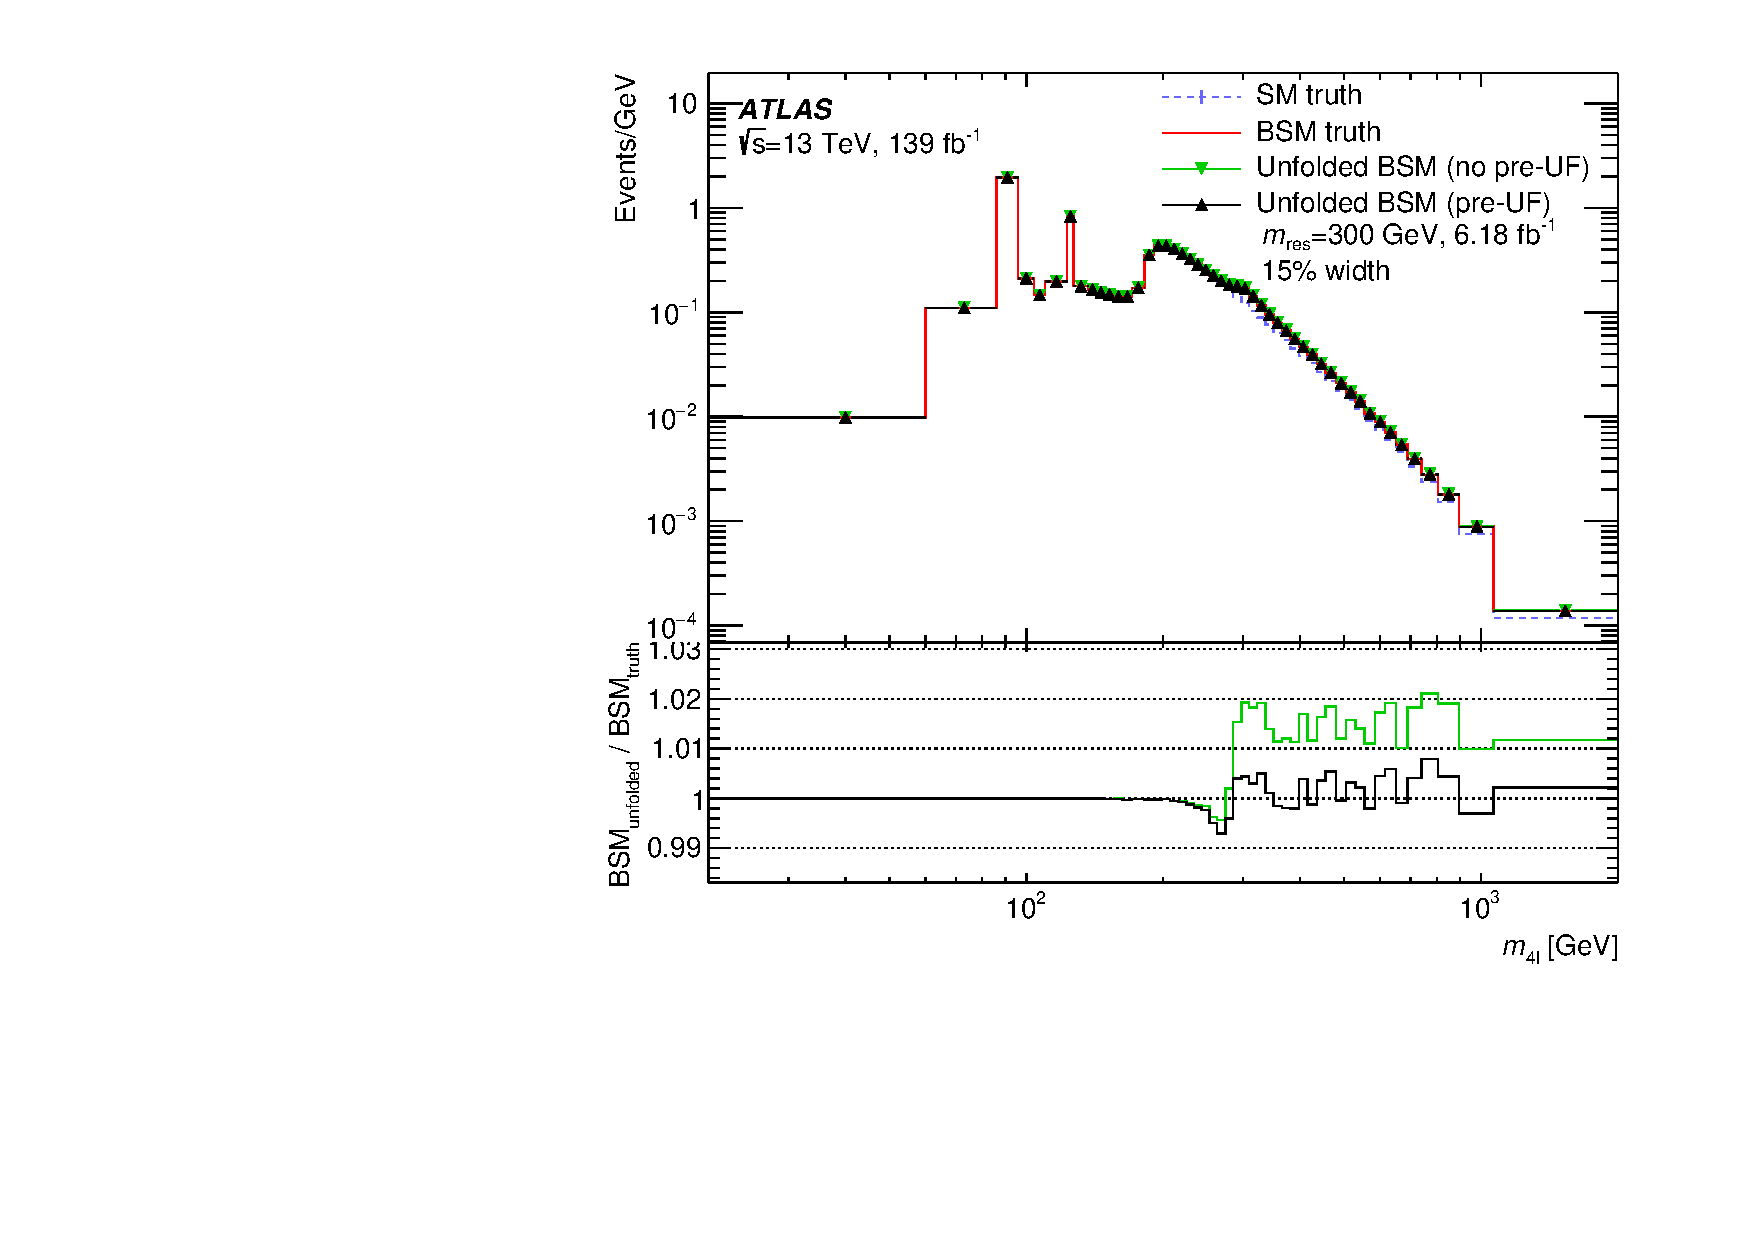
\includegraphics[width = 0.95\textwidth]{Figures/m4l/InjectionTests/6dot175fb_300w15_injection.pdf}\caption{}\label{fig:injection_6dot175fb_300w15}\end{subfigure}
    \begin{subfigure}{.49\textwidth}\centering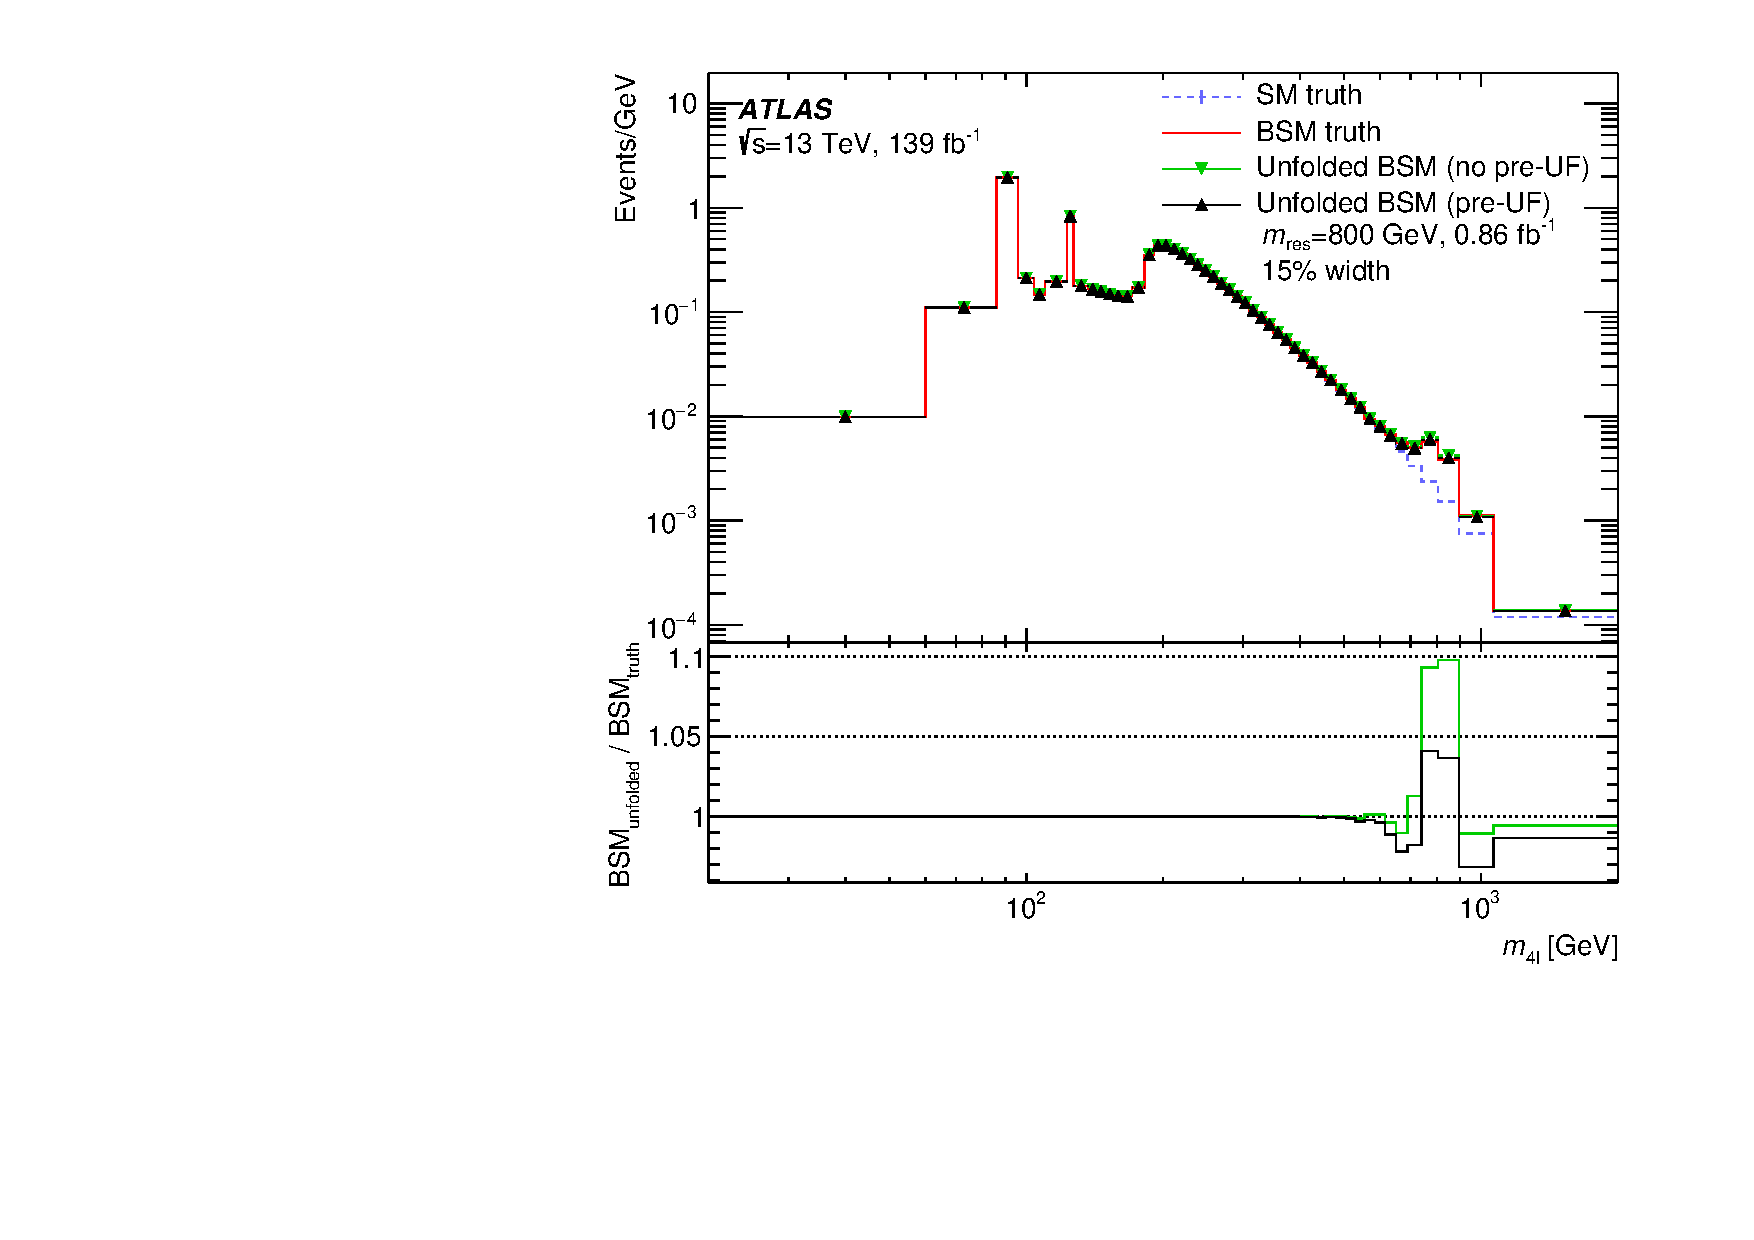
\includegraphics[width = 0.95\textwidth]{Figures/m4l/InjectionTests/0dot862fb_800w15_injection.pdf}\caption{}\label{fig:injection_0dot862fb_800w15}\end{subfigure}
    \begin{subfigure}{.49\textwidth}\centering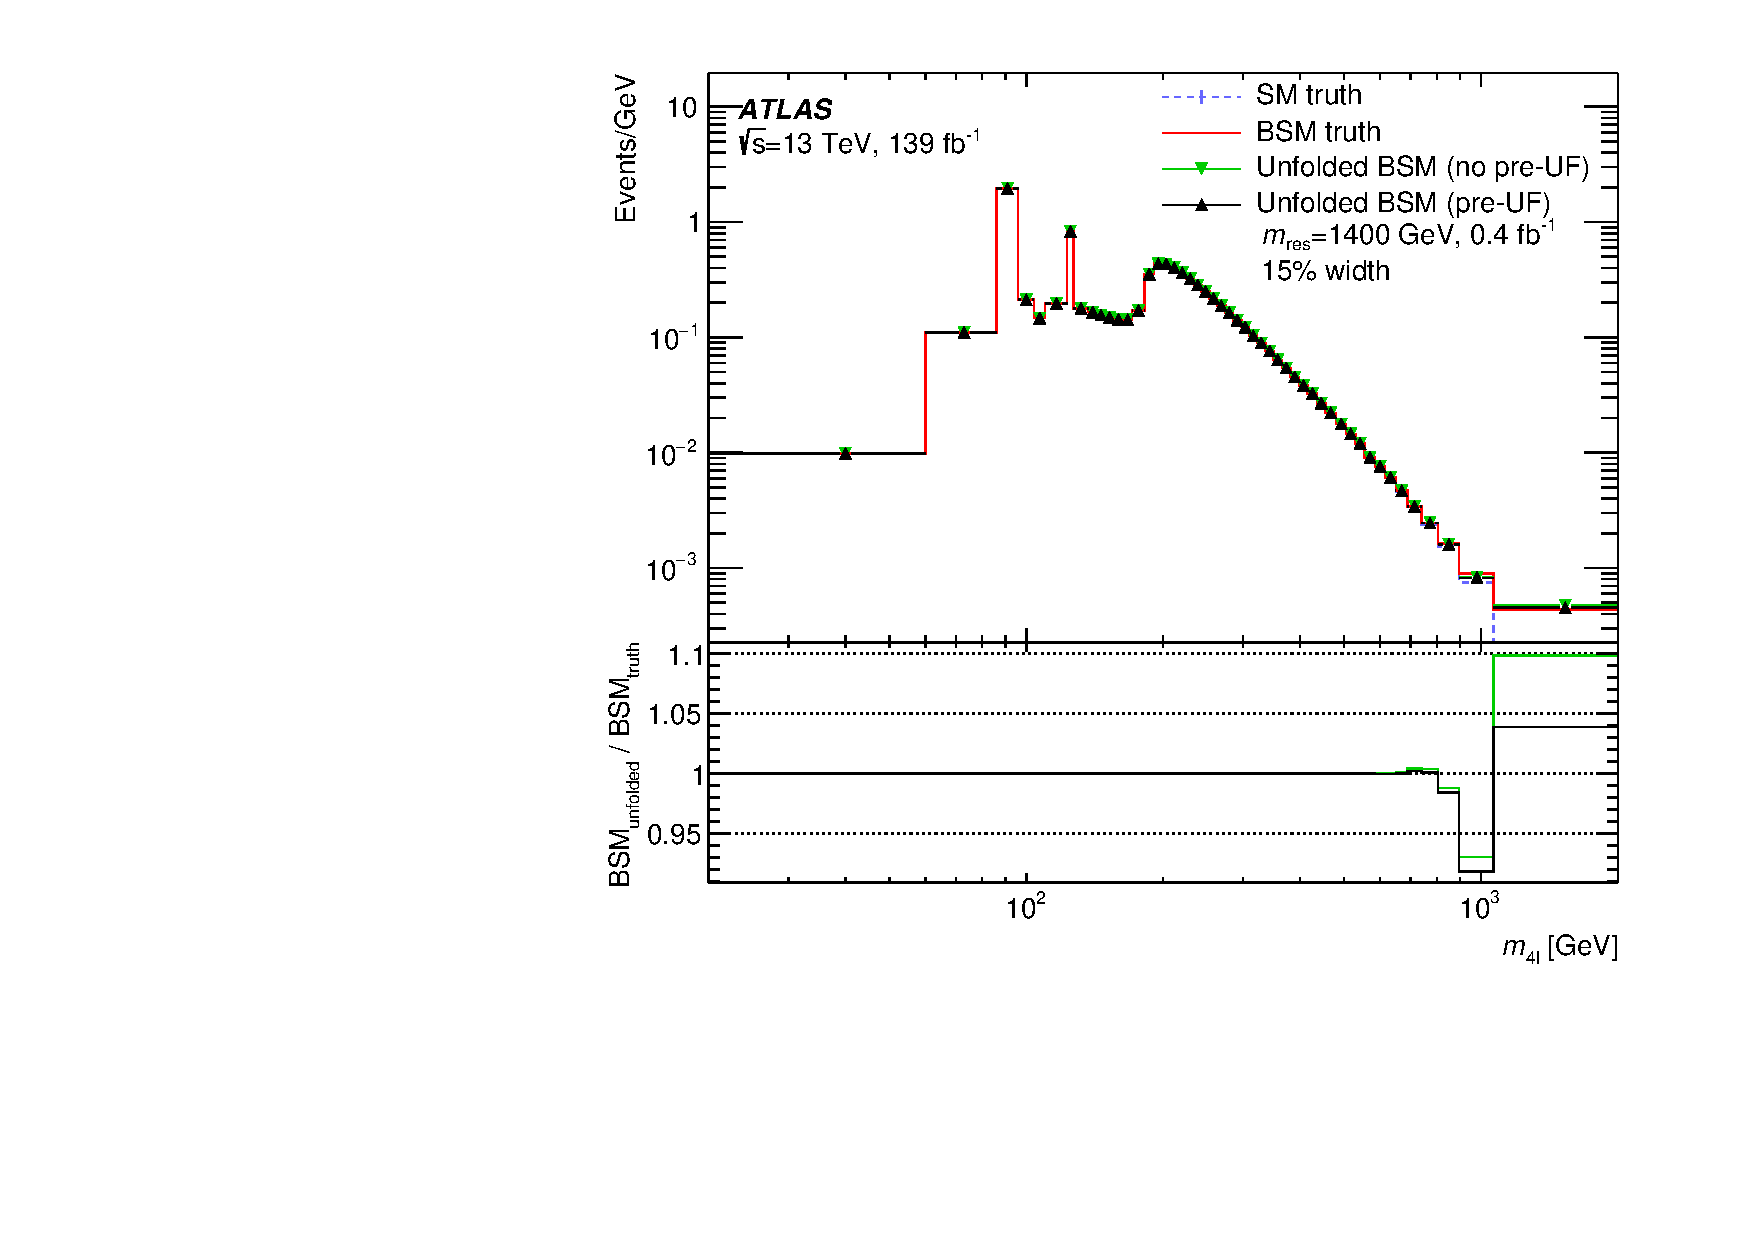
\includegraphics[width = 0.95\textwidth]{Figures/m4l/InjectionTests/0dot4032fb_1400w15_injection.pdf}\caption{}\label{fig:injection_0dot4032fb_1400w15}\end{subfigure}
    \begin{subfigure}{.49\textwidth}\centering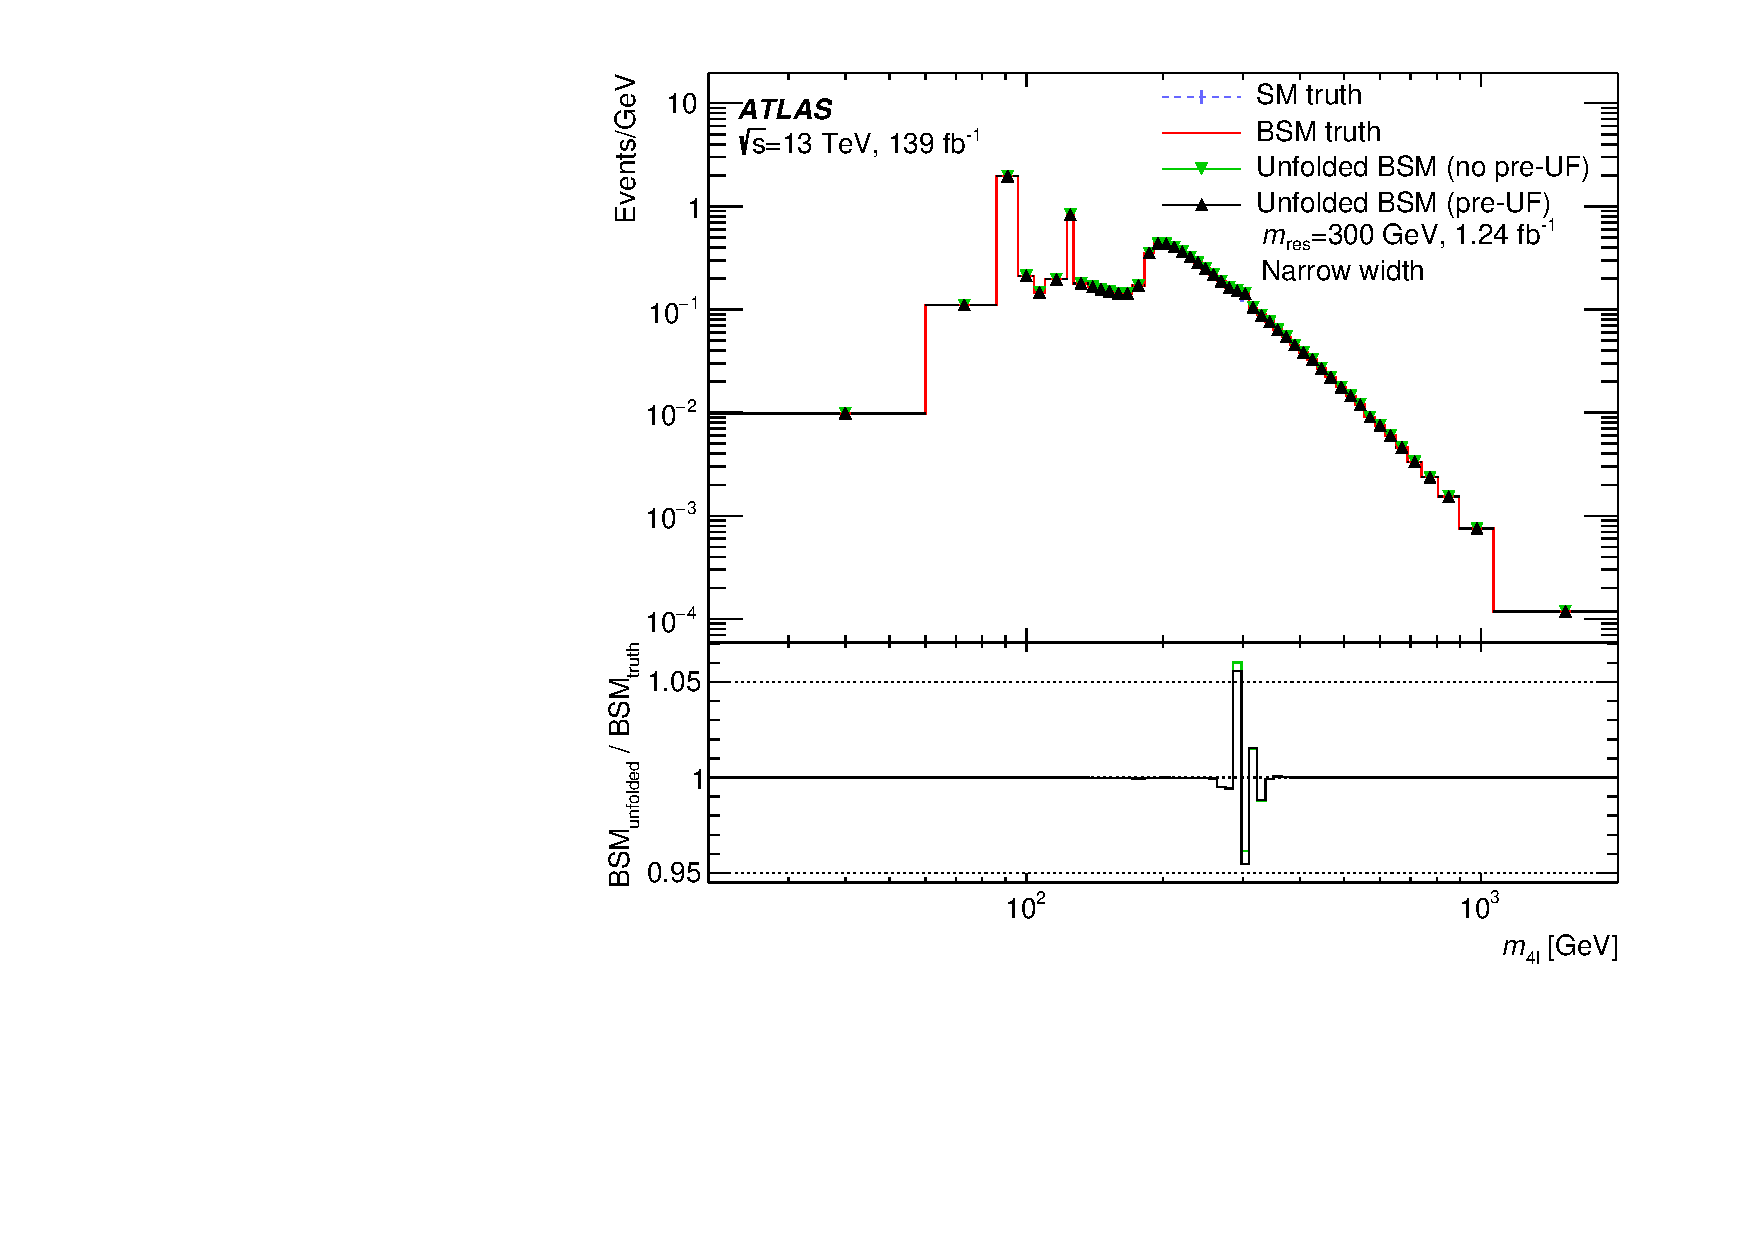
\includegraphics[width = 0.95\textwidth]{Figures/m4l/InjectionTests/1dot24fb_300NW_injection.pdf}\caption{}l\label{fig:injection_1dot24fb_300NW}\end{subfigure}
    \begin{subfigure}{.49\textwidth}\centering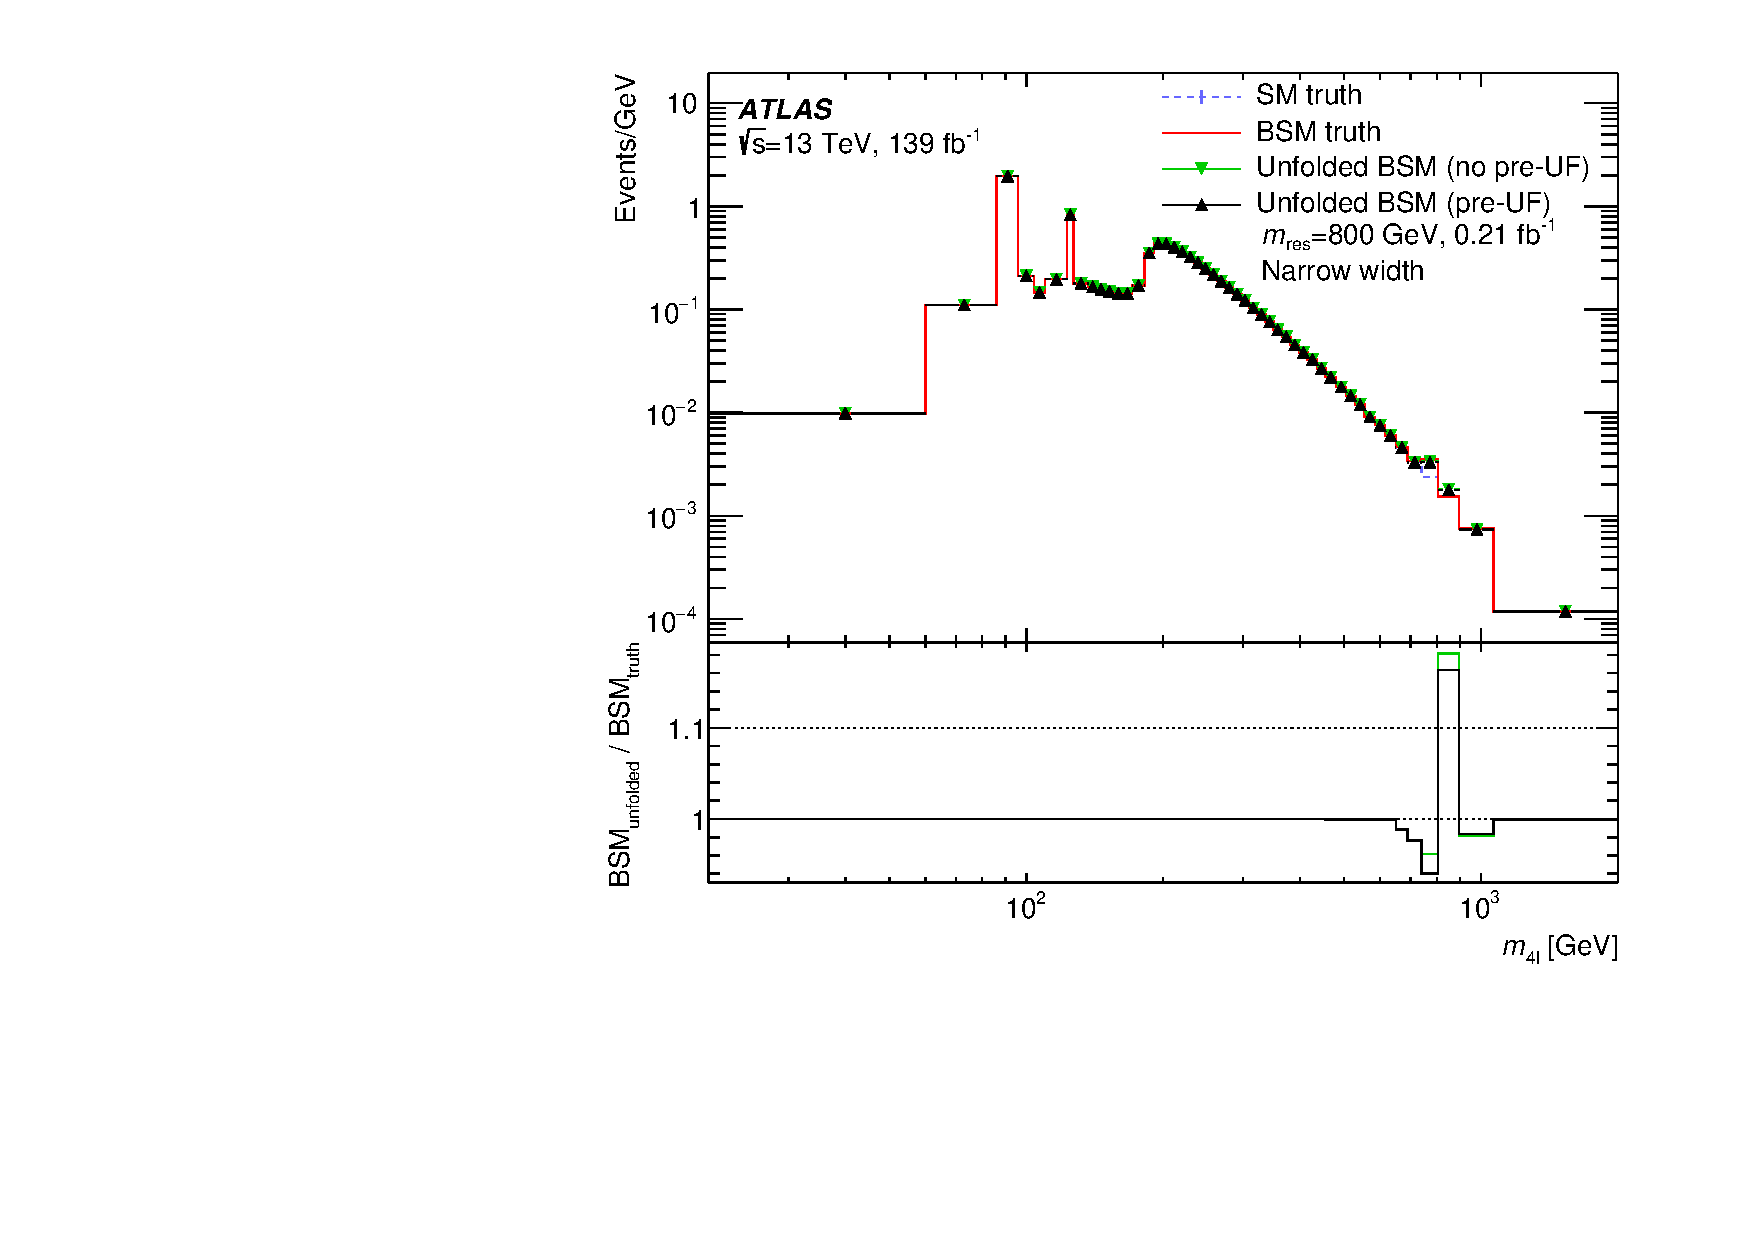
\includegraphics[width = 0.95\textwidth]{Figures/m4l/InjectionTests/0dot212fb_800NW_injection.pdf}\caption{}\end{subfigure}
    \begin{subfigure}{.49\textwidth}\centering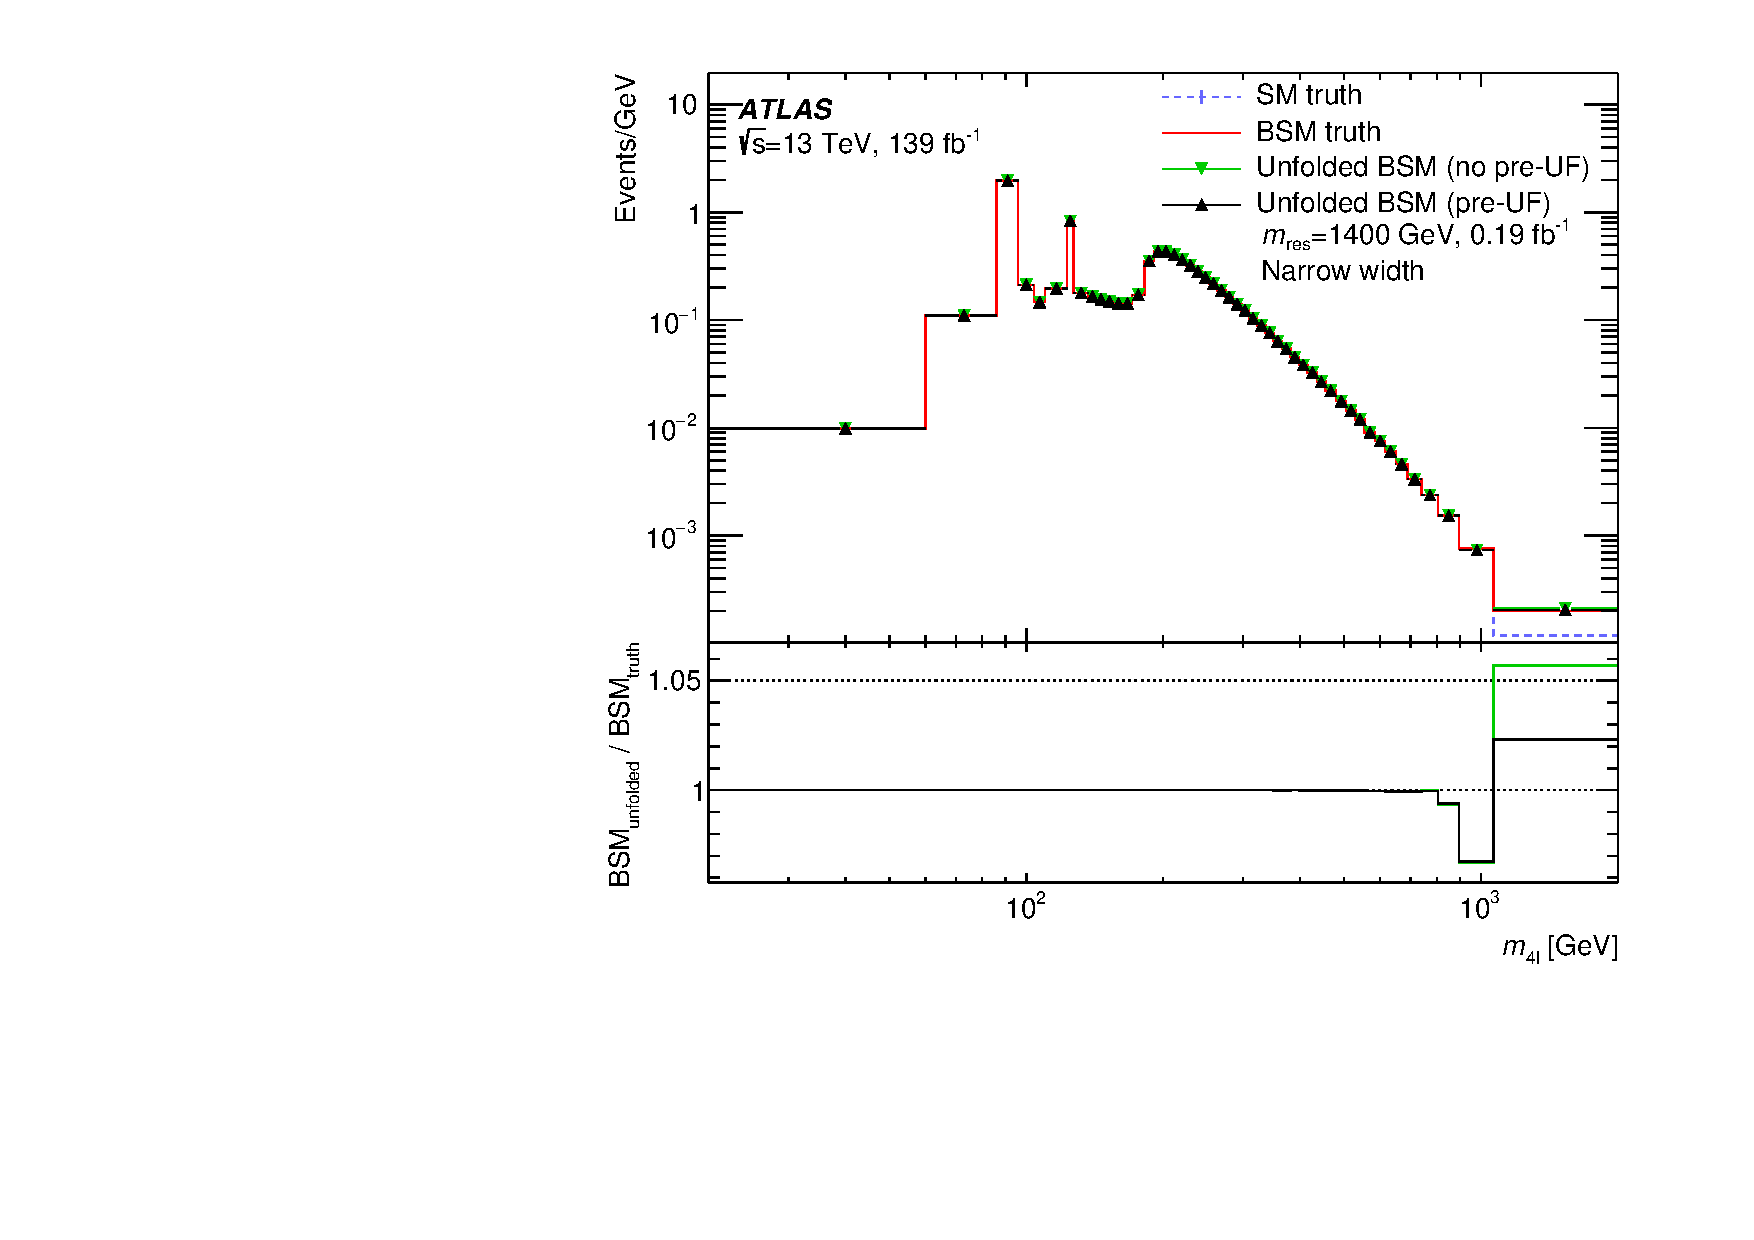
\includegraphics[width = 0.95\textwidth]{Figures/m4l/InjectionTests/0dot19fb_1400NW_injection.pdf}\caption{}\label{fig:injection_0dot19fb_1400NW}\end{subfigure}
    \caption{This figure shows the results of the BSM signal injection studies performed on the \mFourL distribution. Six BSM models are considered, with resonance masses at 300~\GeV, 800~\GeV, and 1400~\GeV, and with narrow widths or a width 15\% of the resonance mass. The cross-sections correspond to a $2\sigma$ signal significant with respect to the data uncertainty. Two unfolded distributions are shown with and without pre-unfolding (pre-UF) weights applied. The bottom panel shows the size of the bias.}
    \label{fig:m4l:injection}
\end{figure}
 \section{Results}
\label{sec:results}
\subsection{Measurements}
\label{ssec:xsecs}



Table~\ref{tab:fidxs} gives the measured cross-sections in the full
fiducial phase space
and in the four \mFourL{} regions, each dominated by different
processes, compared with the
theoretical predictions described in Section~\ref{sec:theory}. Two
predictions are shown, one where the \qqFourL{} process is simulated
with \SHERPA at NLO accuracy in  QCD and one where it is simulated with \POWHEG +
\pythia{} normalised to a prediction at NNLO accuracy in QCD, as
described in Section~\ref{sec:theory}. All the other SM processes are the same in the two
predictions.
The \SHERPA{} prediction is generally higher than the \POWHEG{} +
\pythia{} prediction in all but the on-shell  region, where the
predictions are very close.
The cross-sections measured in data generally agree with both predictions 
within the quoted uncertainties.
The data central values are above the  \POWHEG{} +
\pythia{} predictions in all regions, and
in all but the $\Z\rightarrow 4\ell$ region for \SHERPA. In the
on-shell region the \SHERPA{} prediction
is a bit more than $1\sigma$ below the data.
In Ref.~\cite{ATLAS:2020wny} the \HFourL{}  cross-section is measured
by ATLAS 
in a fiducial phase space that differs slightly from the \HFourL{} region measured here. 
The phase space is designed to minimise the contribution
from non-\HFourL{} processes.
In the dedicated Higgs measurement the cross-section is 
found to be slightly below the SM prediction. The dedicated Higgs measurement 
differs from the present measurement in using a slightly different phase space, in subtracting
non-Higgs processes using a data-driven approach, and in including a $\sim1\%$ 
contribution from  Higgs production in association with a $b$-quark pair in the prediction.

\begin{table}[t] 
  \centering
   \caption{Fiducial cross-sections in femtobarns in the full fiducial phase space and in the
      following regions of
      $\mFourL$: \ZFourL{}  ($60 < \mFourL < 100$~\GeV), \HFourL{}  ($120 <
\mFourL < 130$~\GeV), off-shell $\Z\Z$  ($20 <
\mFourL < 60$~\GeV\ or $100 <
\mFourL < 120$~\GeV\ or $130 <
\mFourL < 180$~\GeV) and  on-shell \Z\Z{} ($180 <
\mFourL < 2000$~\GeV), compared with particle-level predictions and their
    uncertainties as described in Section~\ref{sec:theory}. Two
    predictions are shown for the
    \qqFourL{} process simulated with 
    \SHERPA{} or with \POWHEG{} + \pythia{}. All other SM processes are the
    same for the two predictions. \label{tab:fidxs} }
    \begin{tabular} {c c c c c c }
      \hline
      & \multicolumn{5}{c}{Region} \\
      & Full   & $Z\rightarrow 4\ell$  & \HFourL{}  & Off-shell $ZZ$  & On-shell $ZZ$   \\
      \hline
      Measured        & 88.9              & 22.1              & 4.76                & 12.4                & 49.3 \\
      fiducial & $\pm$1.1 (stat.\,)    & $\pm$0.7 (stat.\,)    &  $\pm$0.29 (stat.\,)  & $\pm$0.5 (stat.\,)     & $\pm$0.8 (stat.\,) \\
      cross-section        & $\pm$2.3 (syst.\,)    & $\pm$1.1 (syst.\,)    &   $\pm$0.18 (syst.\,) & $\pm$0.6 (syst.\,)     & $\pm$0.8 (syst.\,) \\
      $[$fb$]$ 			         & $\pm$1.5 (lumi.)    & $\pm$0.4  (lumi.)  & $\pm$0.08 (lumi.)	   & $\pm$0.2 (lumi.)	   &   $\pm$0.8 (lumi.) \\
                              & $\pm$3.0 (total\,)   & $\pm$1.3 (total\,)   &   $\pm$0.35  (total\,)   & $\pm$0.8 (total\,)    &   $\pm$1.3 (total\,) \\
      \hline
      \SHERPA{}                            & 86$\pm$5          & 23.6$\pm$1.5      & 4.57$\pm$0.21       & 11.5$\pm$0.7       & 46.0$\pm$2.9 \\
      \POWHEG + \pythia{}         & 83$\pm$5          & 21.2$\pm$1.3      & 4.38$\pm$0.20       & 10.7$\pm$0.7       & 46.4$\pm$3.0 \\
      \hline
   \end{tabular}
\end{table}
The differential cross-section as a function of  \mFourL{} is shown in
Figure~\ref{fig:cross-sec-m4l}, in much
finer bins than those in Table~\ref{tab:fidxs}.
The breakdown of the contribution from different SM processes is also
shown.
The features seen in the reconstruction-level distribution in
Figure~\ref{fig:recoresults1} are also
present here.
The SM predictions agree well with the measurement within
uncertainties over the
entire \mFourL{} spectrum, with the same features seen as in the
comparisons in Table~\ref{tab:fidxs}.
For this distribution, and all the others shown below, two $p$-values for the observed data given the predicted SM cross-section
(using either \SHERPA{} or \POWHEG{} to model the \qqFourL{} contribution) are obtained
% from the $\chi^2$. This is defined as $\chi^2 = \left[ \sigdata - \sigpred
% \right] ^T C^{-1} \left[  \sigdata - \sigpred  \right]$, where \sigdata{} and $\sigpred$ are $k$-dimensional vectors from the measured and predicted differential
% cross-sections of a given observable respectively, and $C$ is the $k\times k$ total covariance
% matrix defined by the sum of the statistical and systematic
% covariances in \sigdata{} and \sigpred.
% The statistical
% covariance on \sigdata{}  is obtained from the expected number of SM events, as
described in Section~\ref{sec:unc}.
The $p$-value is the probability for the
$\chi^2$, with $k$ degrees of
freedom,  to have at
least the observed value.

\begin{figure}[tb]
  \centering
  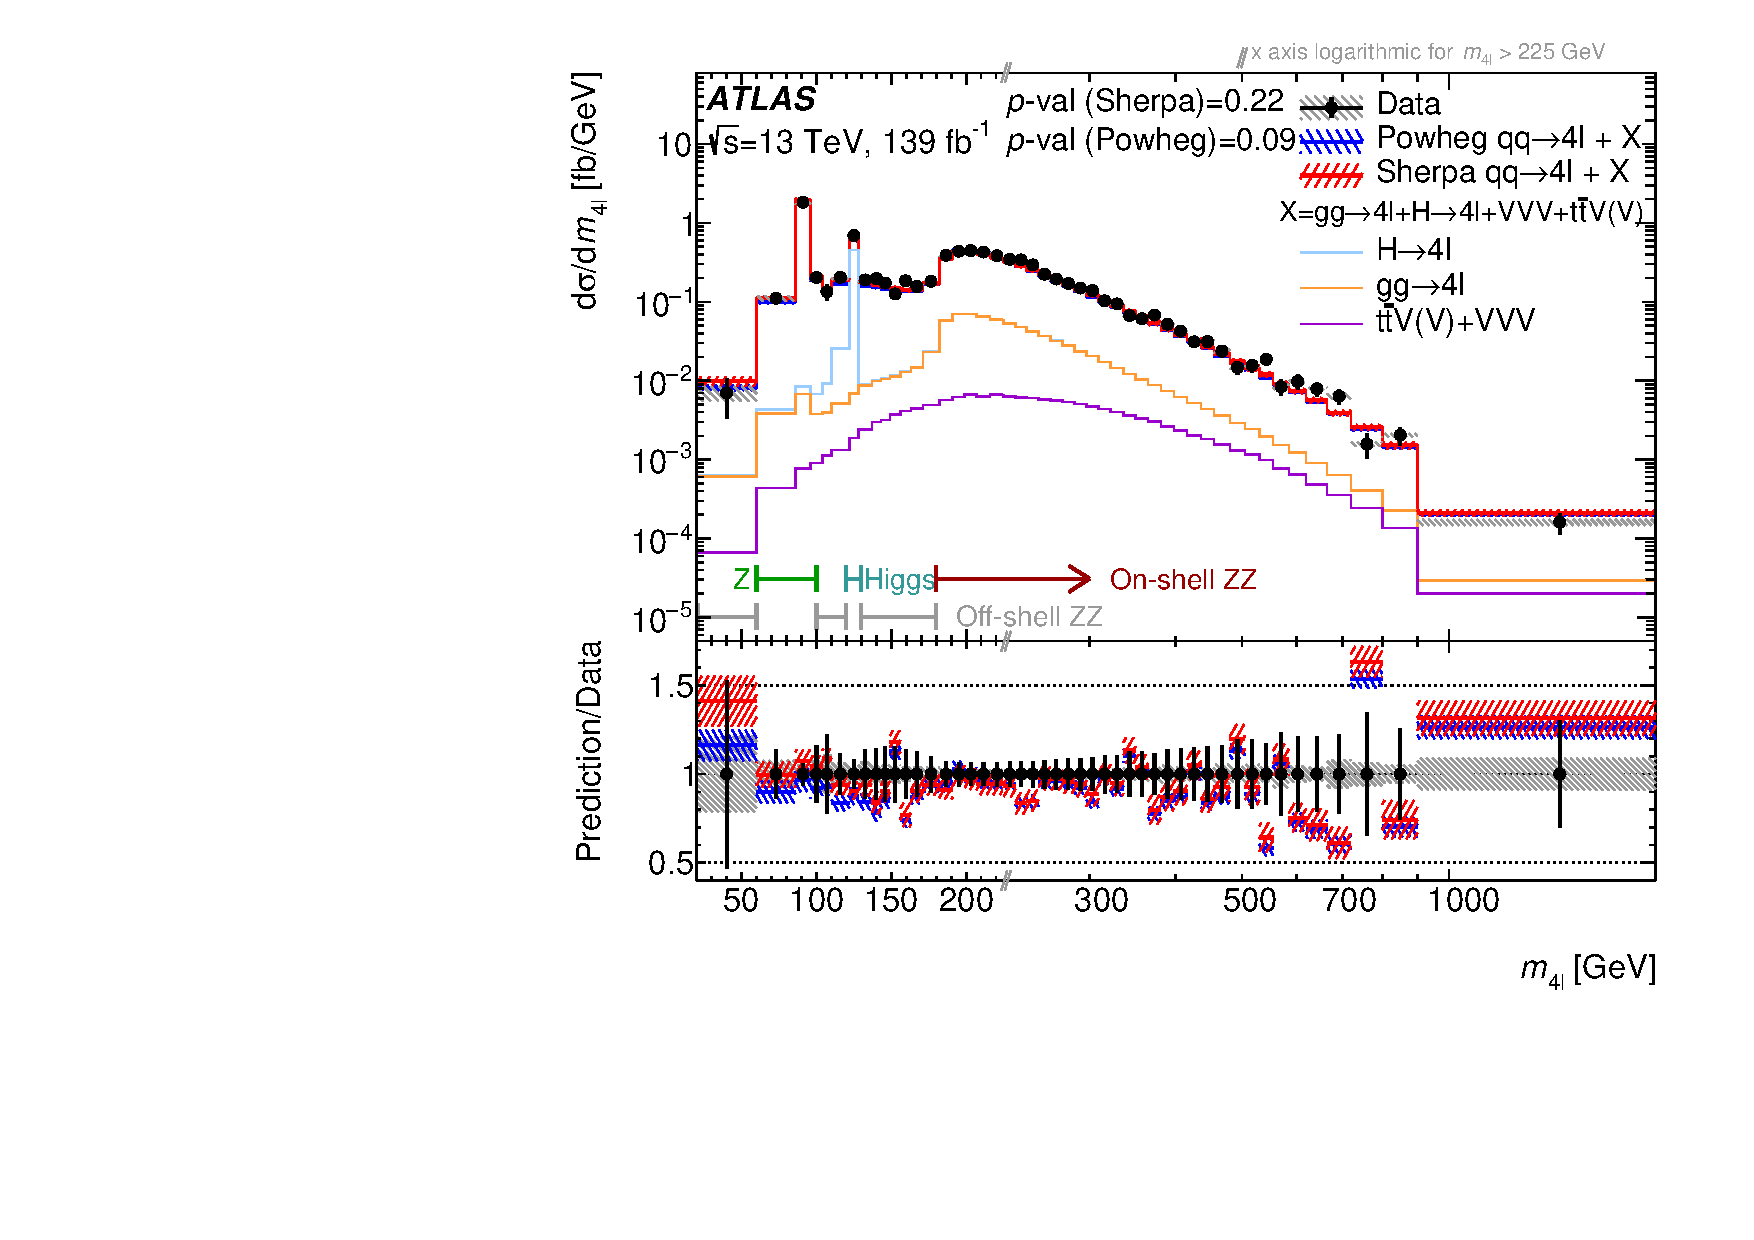
\includegraphics[width = 0.85\textwidth]{Figures/m4l/UnfoldedResults/linlog_Unfolded_Data_inclm4l.pdf} 
    \caption{Differential cross-section as a function of \mFourL. The measured data
  (black points)  are compared with the SM
  prediction using either \SHERPA{} (red, with red hashed
  band for the uncertainty) or \POWHEG{} + \pythia{} (blue,
  with blue hashed band for the uncertainty) to model the \qqFourL{} contribution. The error bars on the data points give the total uncertainty
  and the grey hashed band gives the systematic uncertainty. The
  breakdown of the contribution from different SM processes is also
  shown in successive stacked histograms.
  The short vertical lines terminating horizontal lines indicate the boundaries of the different
  \mFourL{} regions in which the other variables are measured.
  \Pvalue{}
  The
  lower panel shows the ratio of the SM predictions to the 
  data. The $x$-axis is on a linear scale until $\mFourL = 216$~\GeV,
  where it switches to a logarithmic scale. \label{fig:cross-sec-m4l}}
\end{figure}
In order to study the different \mFourL{} regions in more detail,  Figures~\ref{fig:mz1res} and~\ref{fig:mz2res} 
show the cross-section versus 
\mZOne{} and \mZTwo{} respectively in each region.
In the \HFourL{} region the contribution from Higgs production is
shown separately.

%% m4l vs pt4l
\begin{figure}[htb!]
    \begin{subfigure}{.49\textwidth}\centering
      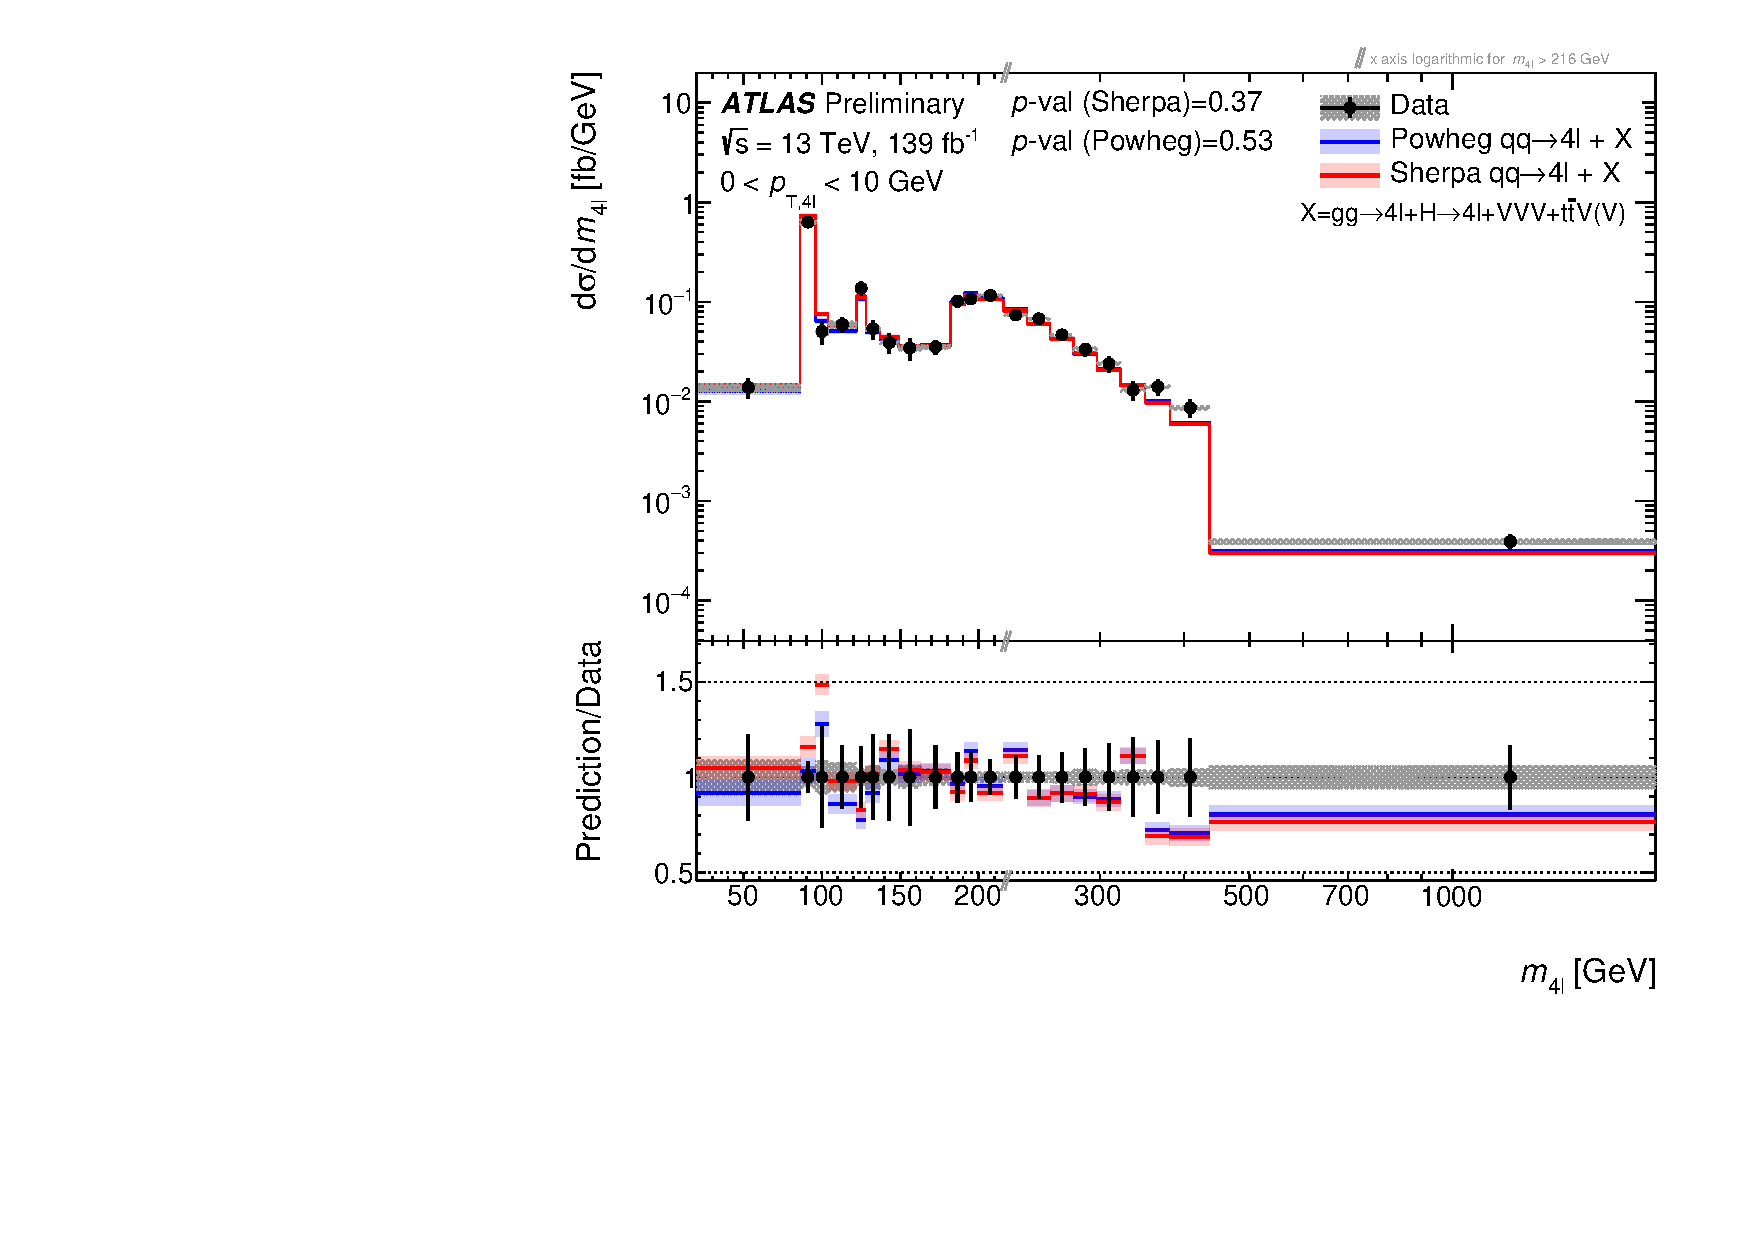
\includegraphics[width=.99\linewidth]{Figures/m4l/UnfoldedResults/linlog_Unfolded_Data_m4l_pt4l0-10.pdf}\caption{$\unit{0}{\GeV} <  \ptFourL  < \unit{10}{\GeV}$}\label{fig:sub-first}
    \end{subfigure}
    \begin{subfigure}{.49\textwidth}\centering
      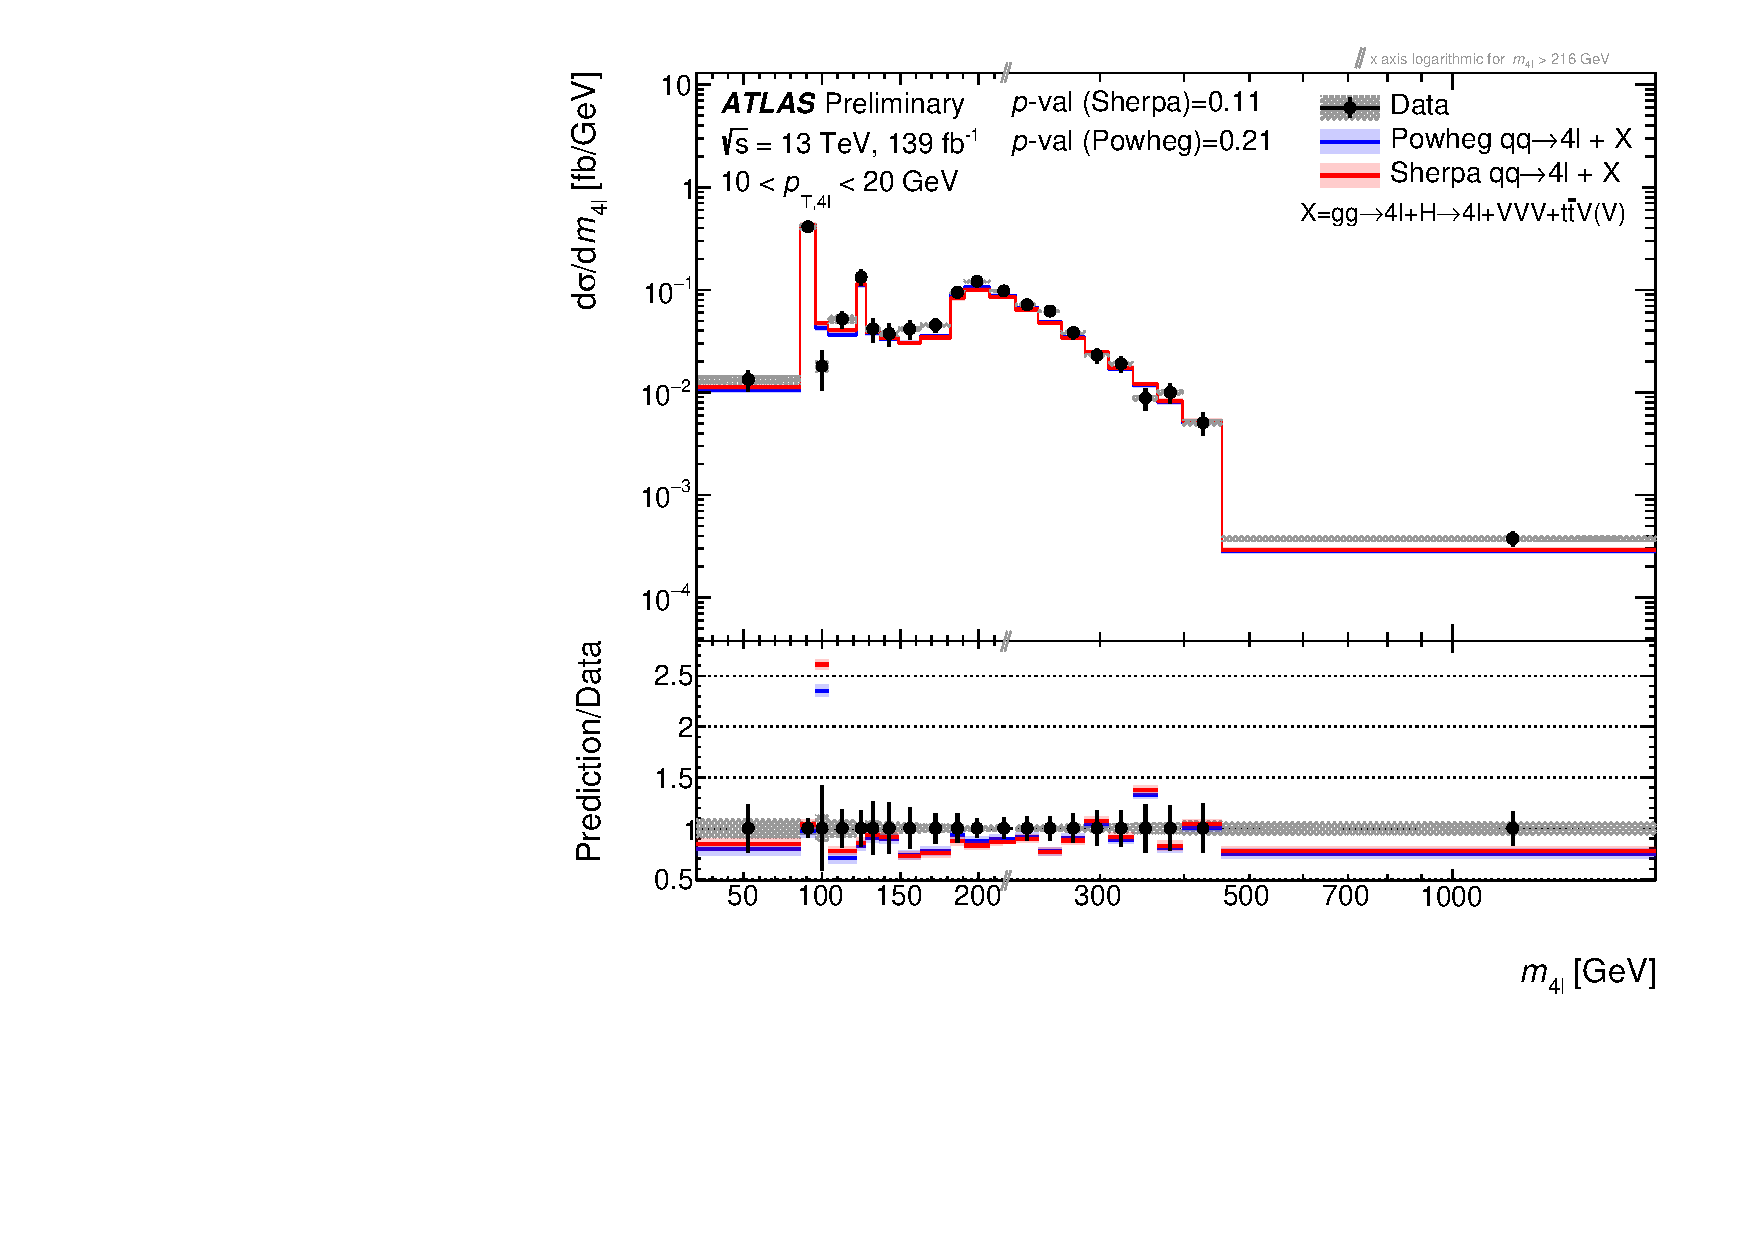
\includegraphics[width=.99\linewidth]{Figures/m4l/UnfoldedResults/linlog_Unfolded_Data_m4l_pt4l10-20.pdf} \caption{$\unit{10}{\GeV} <  \ptFourL  < \unit{20}{\GeV}$}\label{fig:sub-second}
    \end{subfigure}
    \begin{subfigure}{.49\textwidth}\centering
      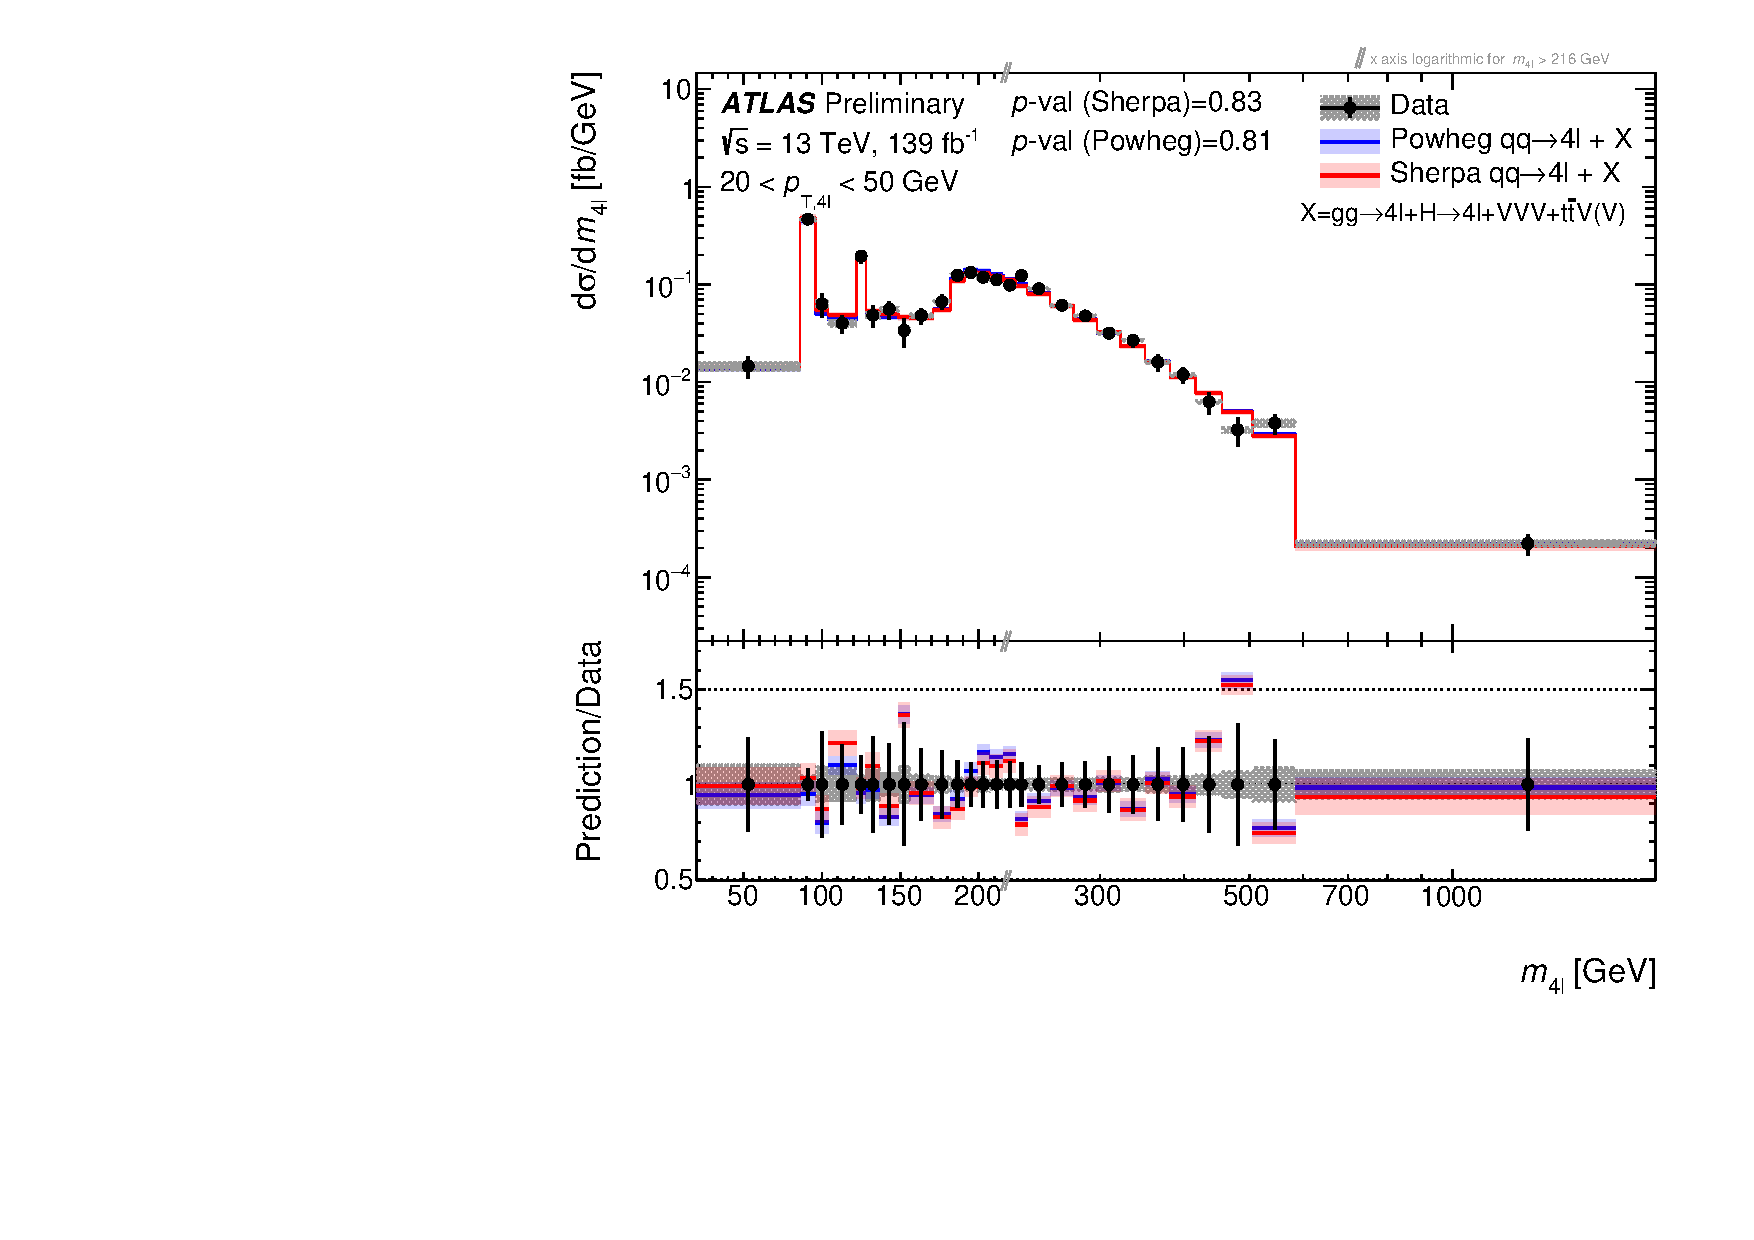
\includegraphics[width=.99\linewidth]{Figures/m4l/UnfoldedResults/linlog_Unfolded_Data_m4l_pt4l20-50.pdf}  \caption{$\unit{20}{\GeV} <  \ptFourL  < \unit{50}{\GeV}$}\label{fig:sub-third}
    \end{subfigure}
    \begin{subfigure}{.49\textwidth}\centering
      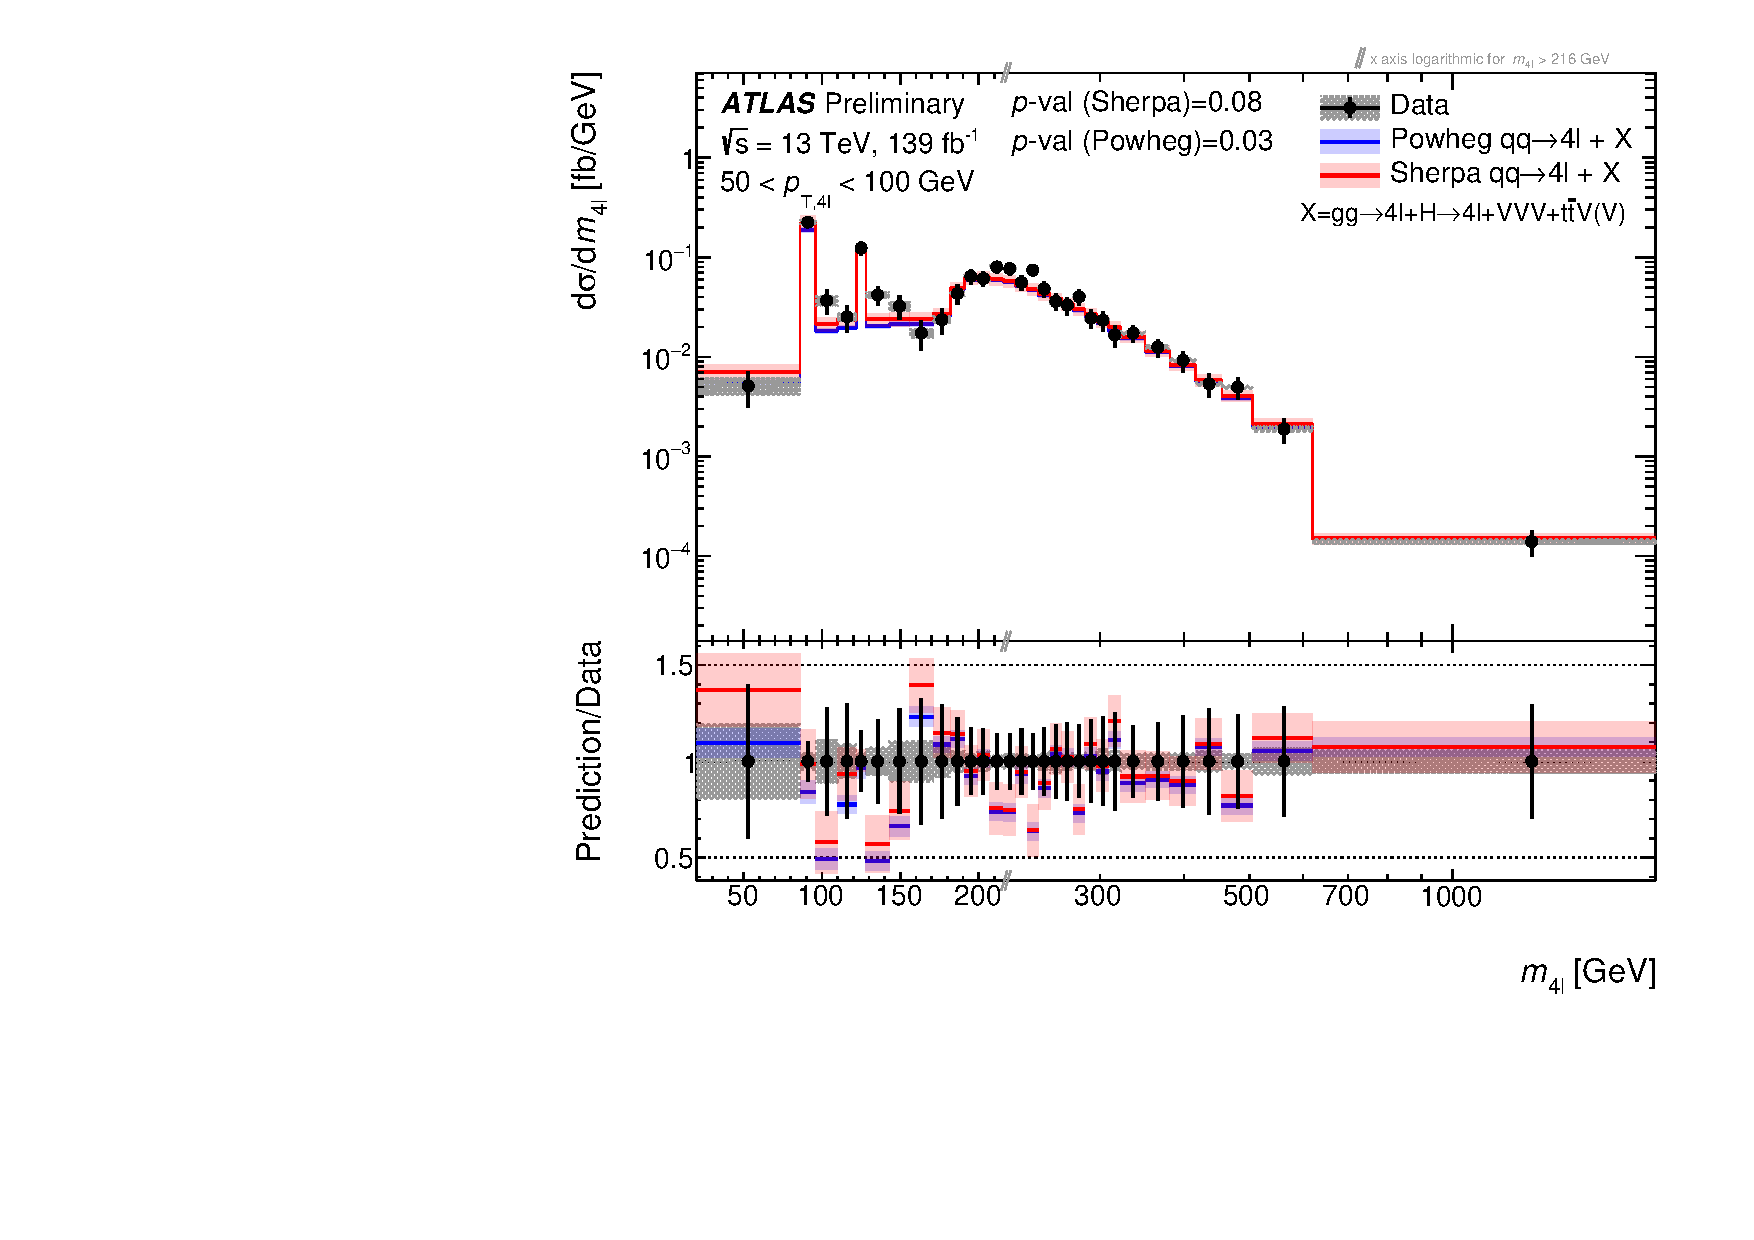
\includegraphics[width=.99\linewidth]{Figures/m4l/UnfoldedResults/linlog_Unfolded_Data_m4l_pt4l50-100.pdf}  \caption{$\unit{50}{\GeV} <  \ptFourL  < \unit{100}{\GeV}$}\label{fig:sub-fourth}
    \end{subfigure}
        \begin{subfigure}{.49\textwidth}\centering
      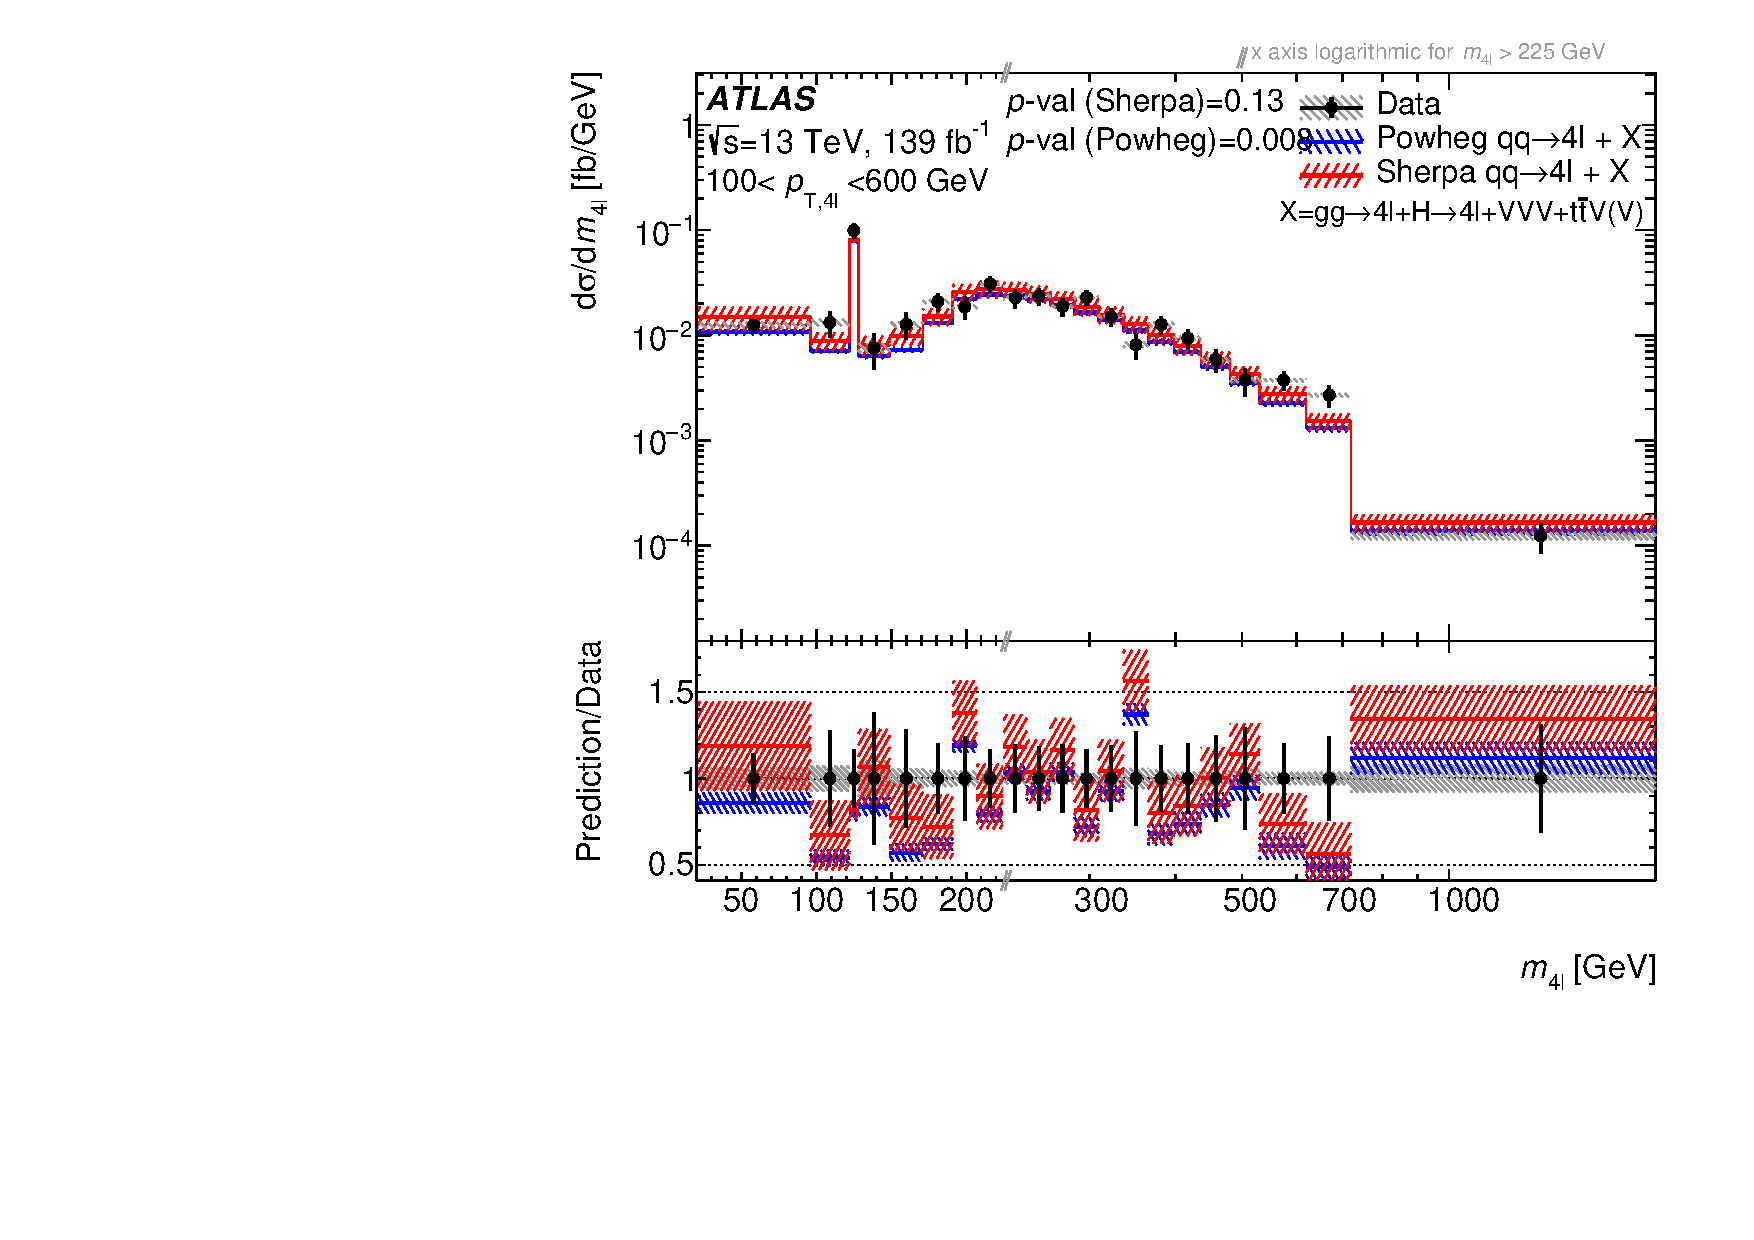
\includegraphics[width=.99\linewidth]{Figures/m4l/UnfoldedResults/linlog_Unfolded_Data_m4l_pt4l100-600.pdf}  \caption{$\unit{100}{\GeV} <  \ptFourL  < \unit{60 0}{\GeV}$}\label{fig:sub-fifth}
    \end{subfigure}
    \caption{Differential cross-section as a function of \mFourL{} in slices of \ptFourL{}. The measured data (black points) are  compared with the SM prediction using either \SHERPA{} (red, with red hashed band for the uncertainty) or \POWHEG{} + \pythia{} (blue, with blue hashed band for the uncertainty) to model the \qqFourL{} contribution. The error bars on the data points give the total uncertainty and the grey hashed band gives the systematic uncertainty. \Pvalue{} The  lower panel shows the ratio of the SM predictions to the data.}
    \label{fig:m4l_pt4l}
\end{figure}

%% m4l vs y4l
\begin{figure}[htb!]
    \begin{subfigure}{.49\textwidth}\centering
      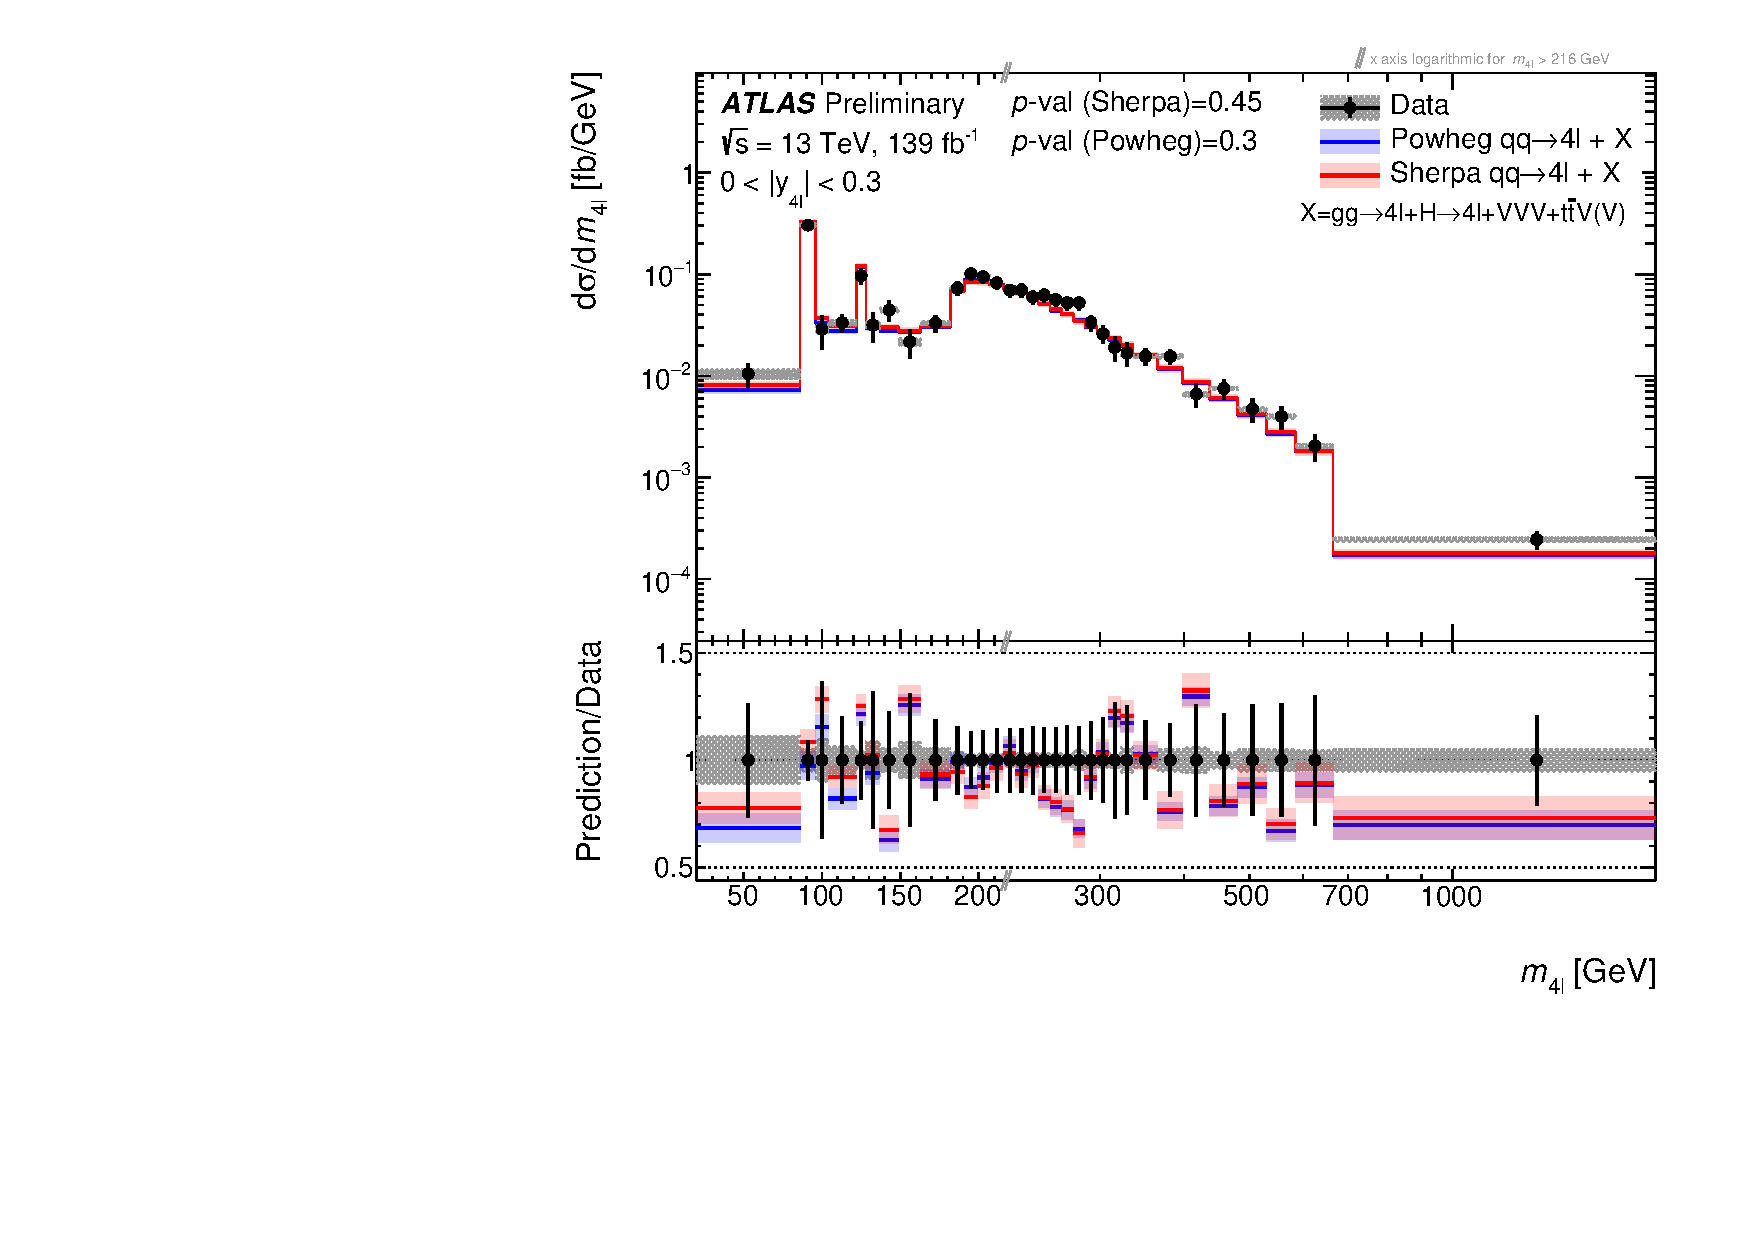
\includegraphics[width=.99\linewidth]{Figures/m4l/UnfoldedResults/linlog_Unfolded_Data_m4l_y4l0-0dot3.pdf}\caption{0 < \yFourL{} < 0.3}\label{fig:sub-first}
    \end{subfigure}
    \begin{subfigure}{.49\textwidth}\centering
      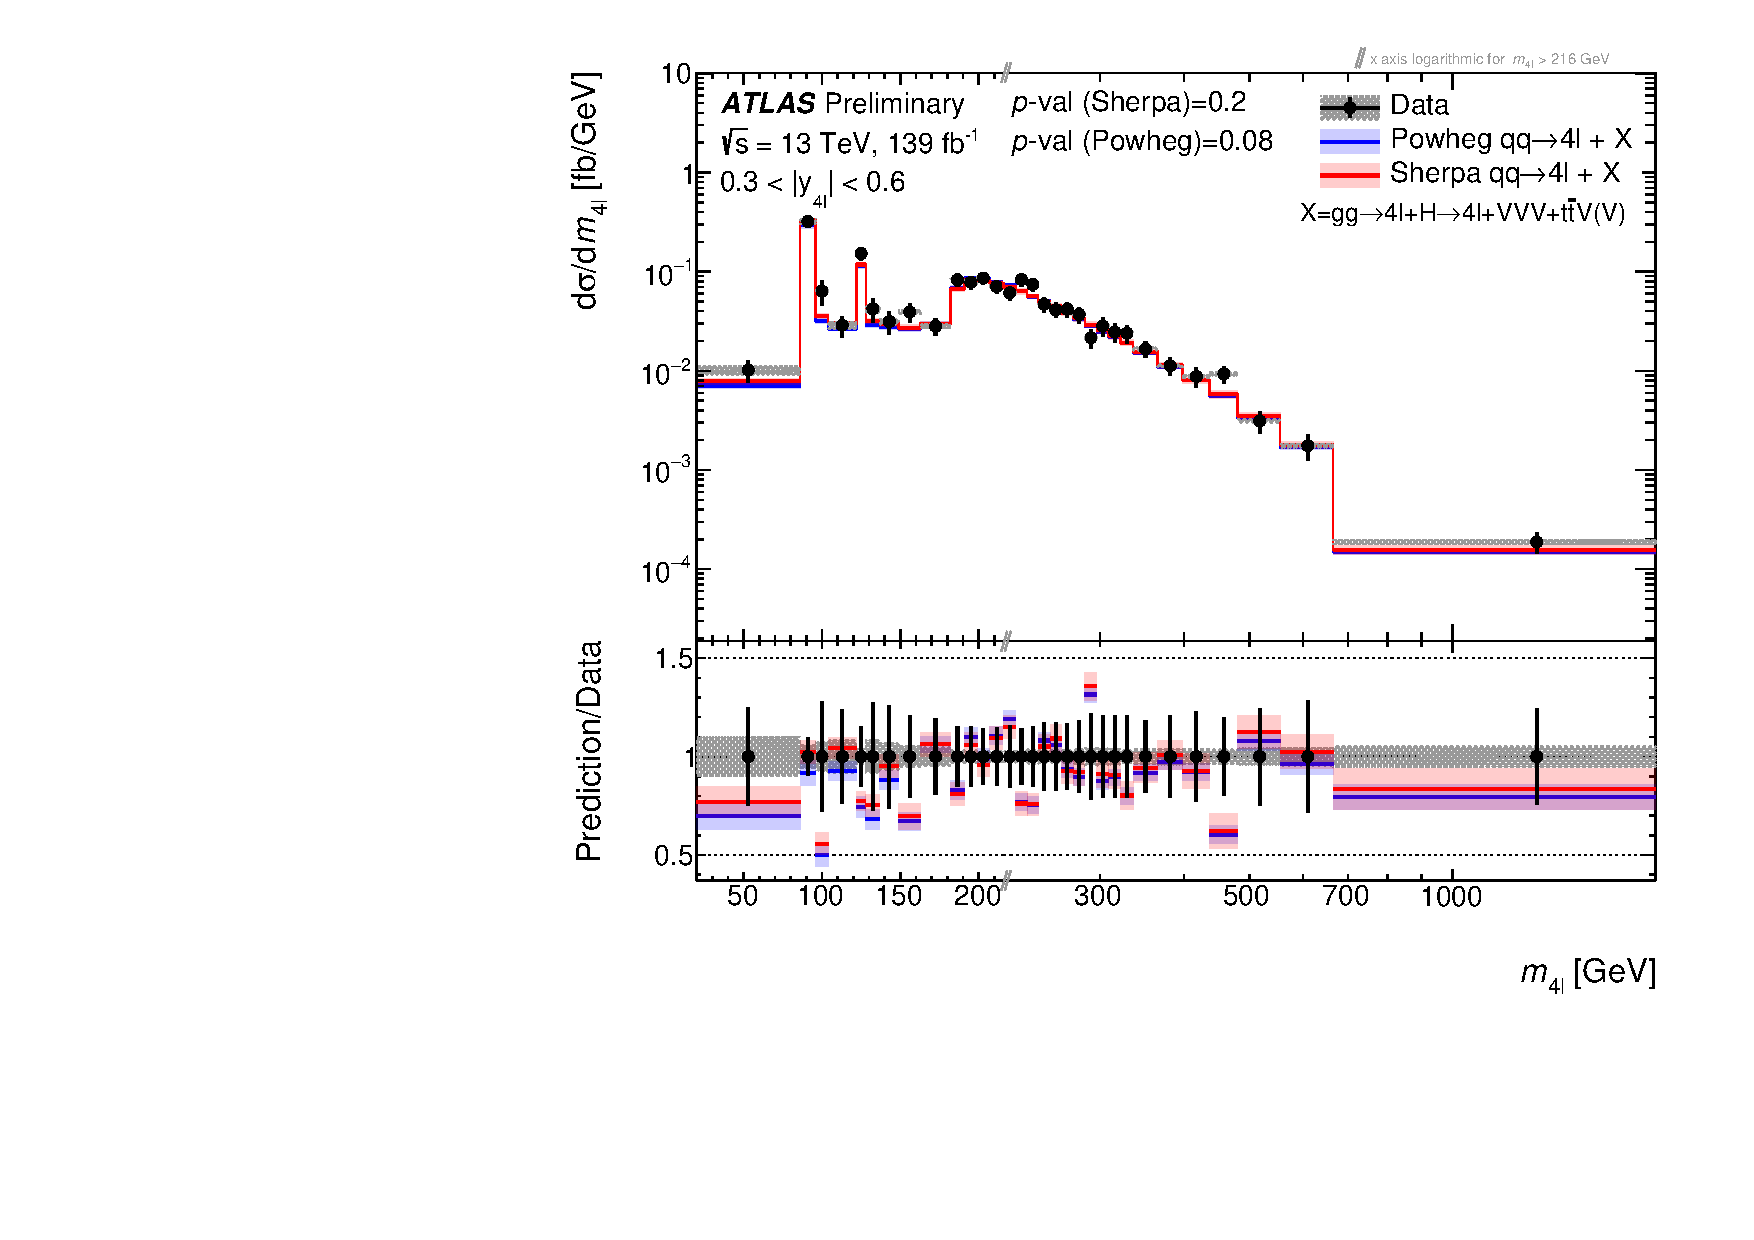
\includegraphics[width=.99\linewidth]{Figures/m4l/UnfoldedResults/linlog_Unfolded_Data_m4l_y4l0dot3-0dot6.pdf} \caption{0.3 < \yFourL{} < 0.6}\label{fig:sub-second}
    \end{subfigure}
    \begin{subfigure}{.49\textwidth}\centering
      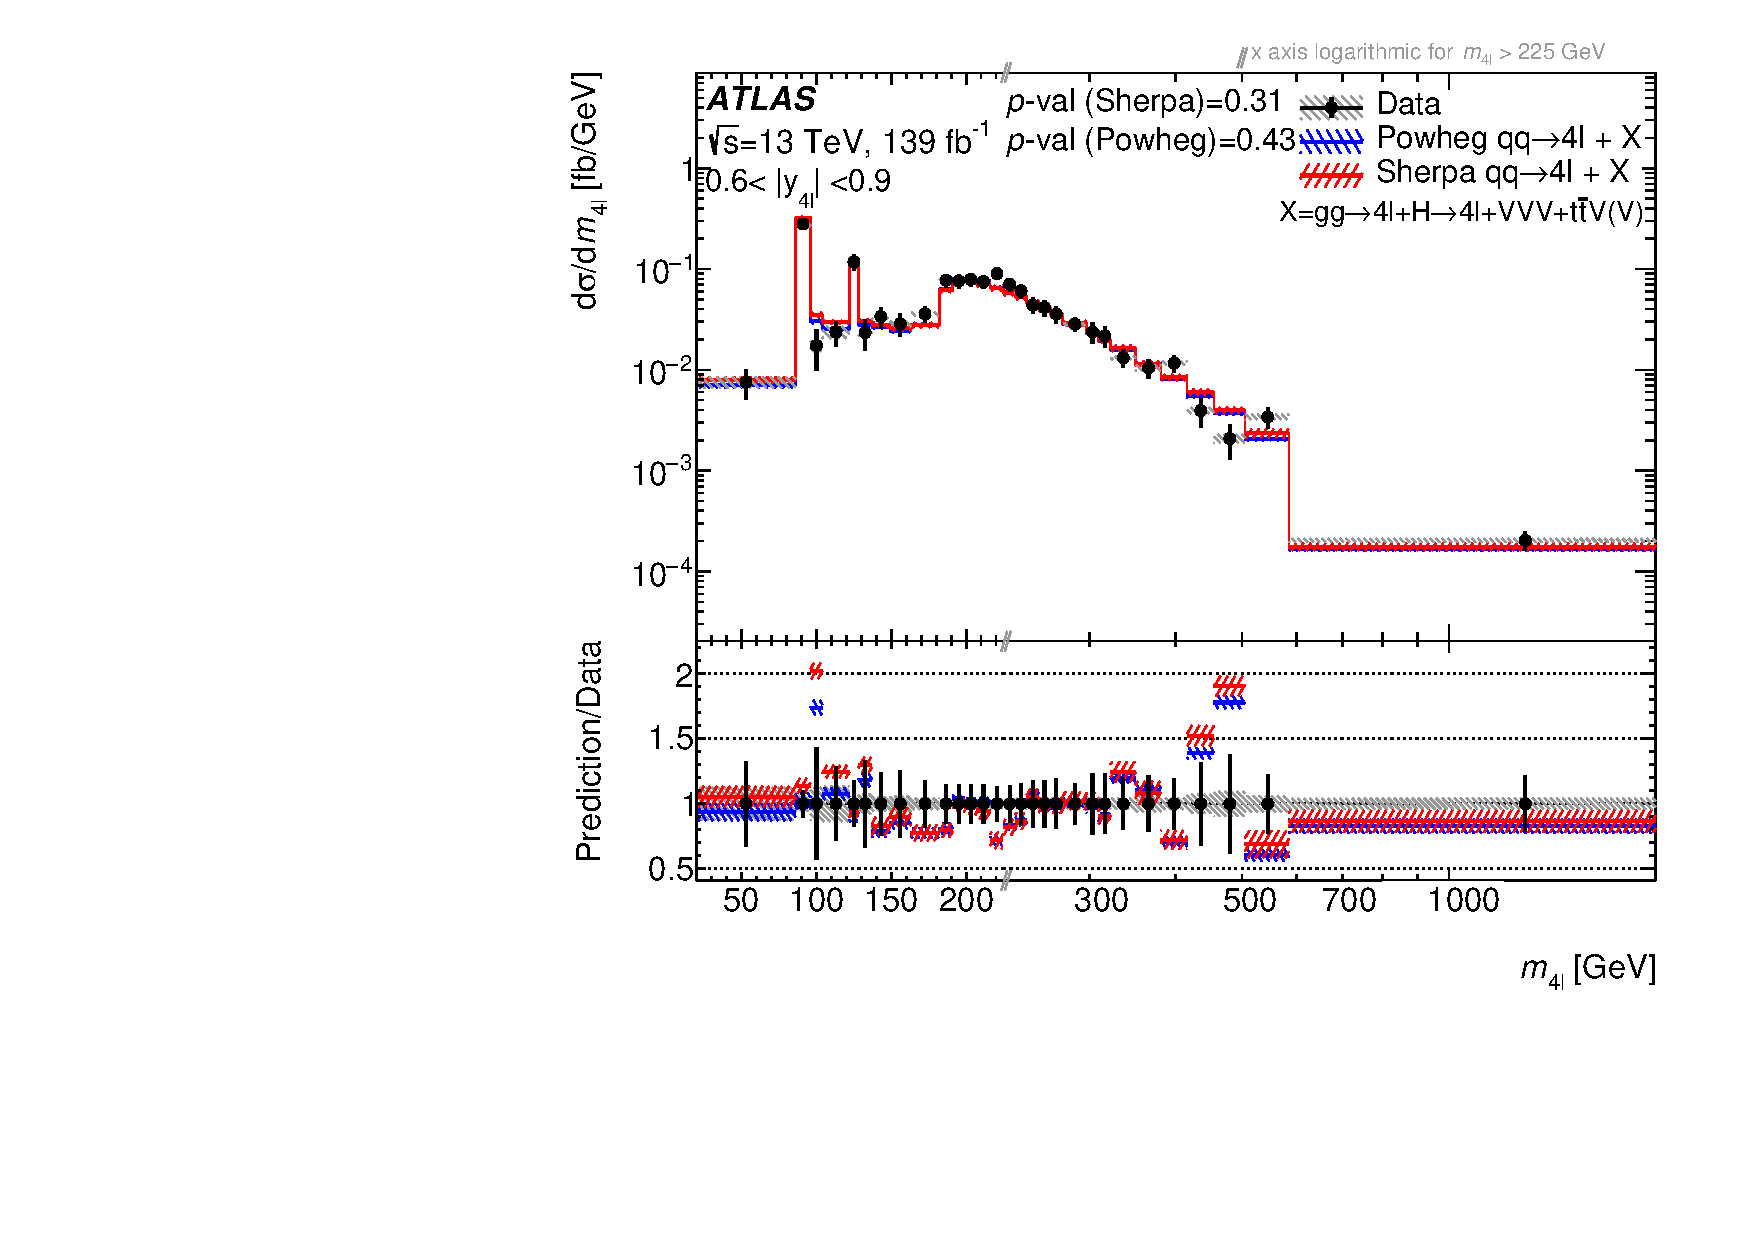
\includegraphics[width=.99\linewidth]{Figures/m4l/UnfoldedResults/linlog_Unfolded_Data_m4l_y4l0dot6-0dot9.pdf}  \caption{0.6 < \yFourL{} < 0.9}\label{fig:sub-third}
    \end{subfigure}
    \begin{subfigure}{.49\textwidth}\centering
      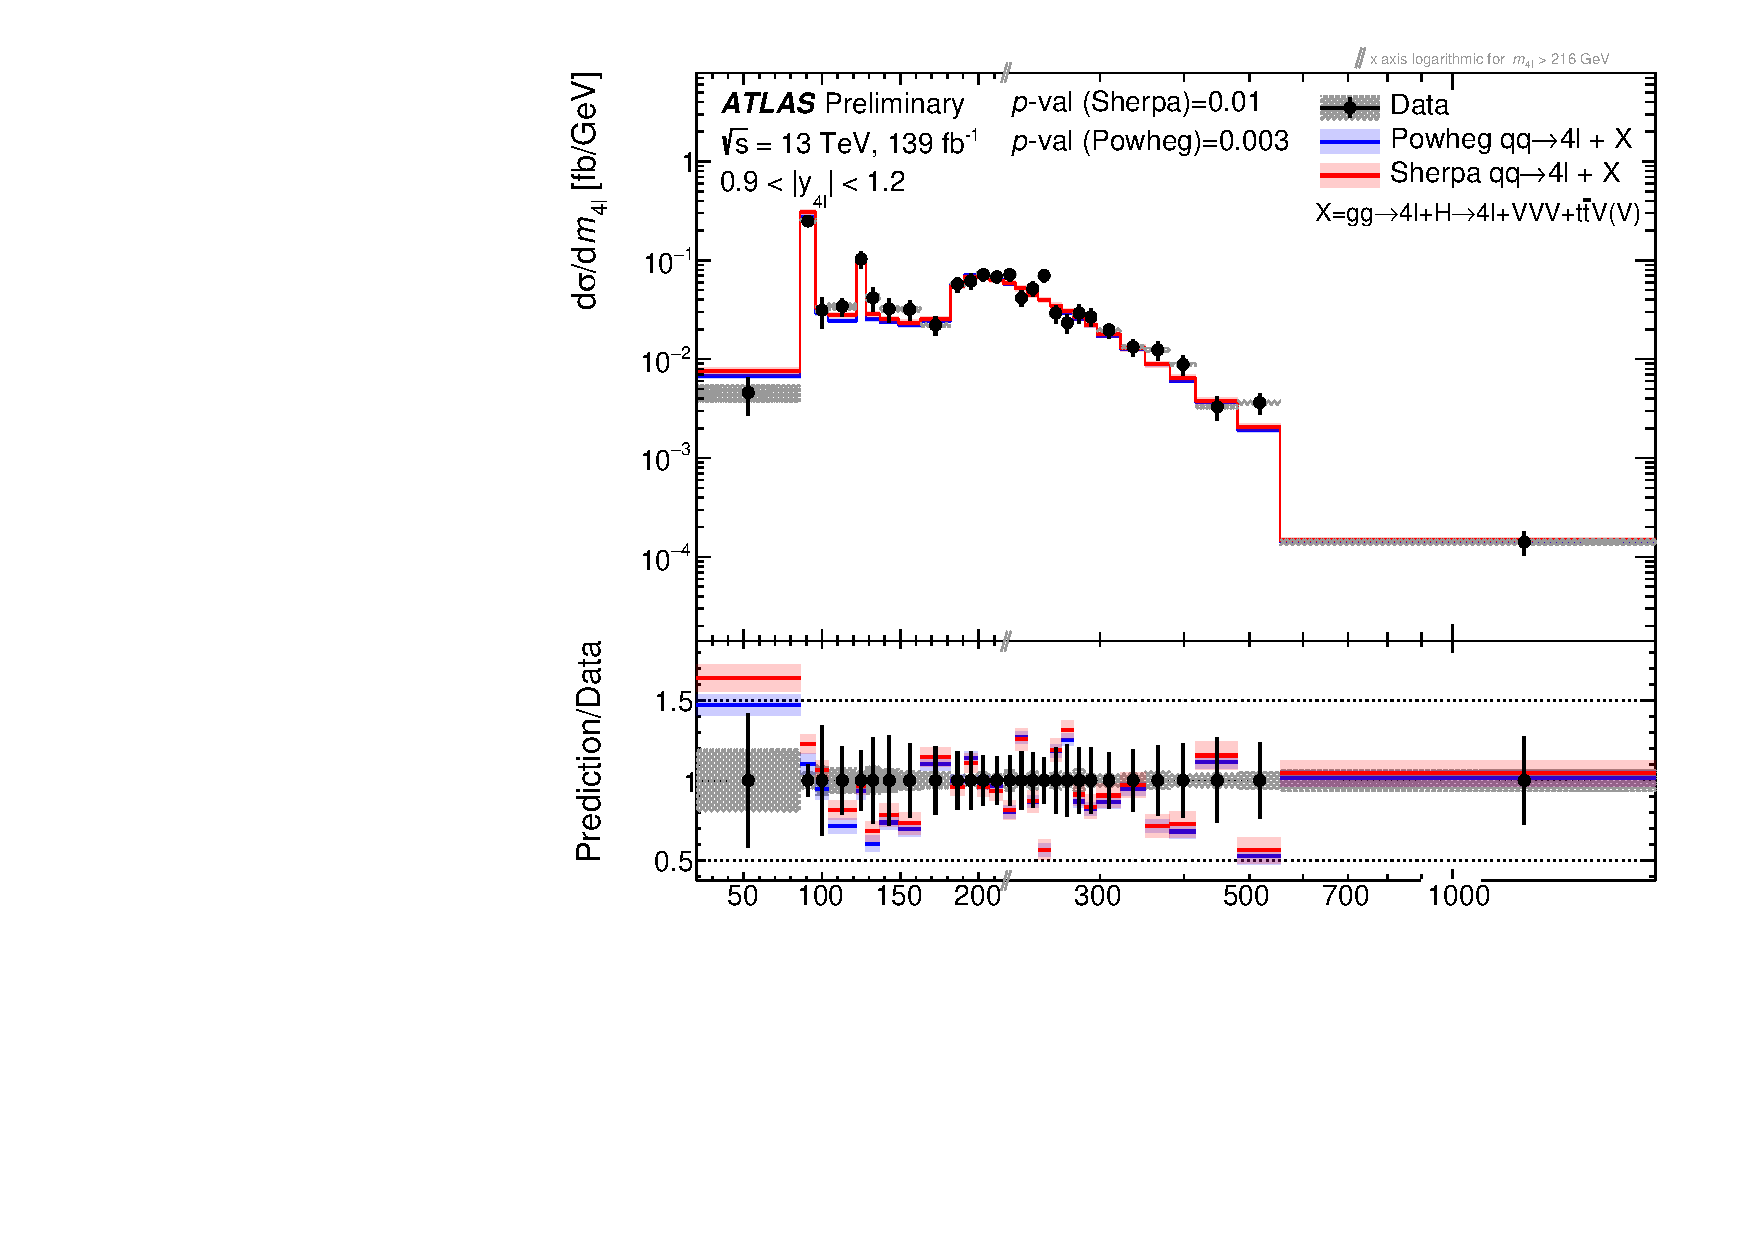
\includegraphics[width=.99\linewidth]{Figures/m4l/UnfoldedResults/linlog_Unfolded_Data_m4l_y4l0dot9-1dot2.pdf}  \caption{0.9 < \yFourL{} < 1.2}\label{fig:sub-fourth}
    \end{subfigure}
        \begin{subfigure}{.49\textwidth}\centering
      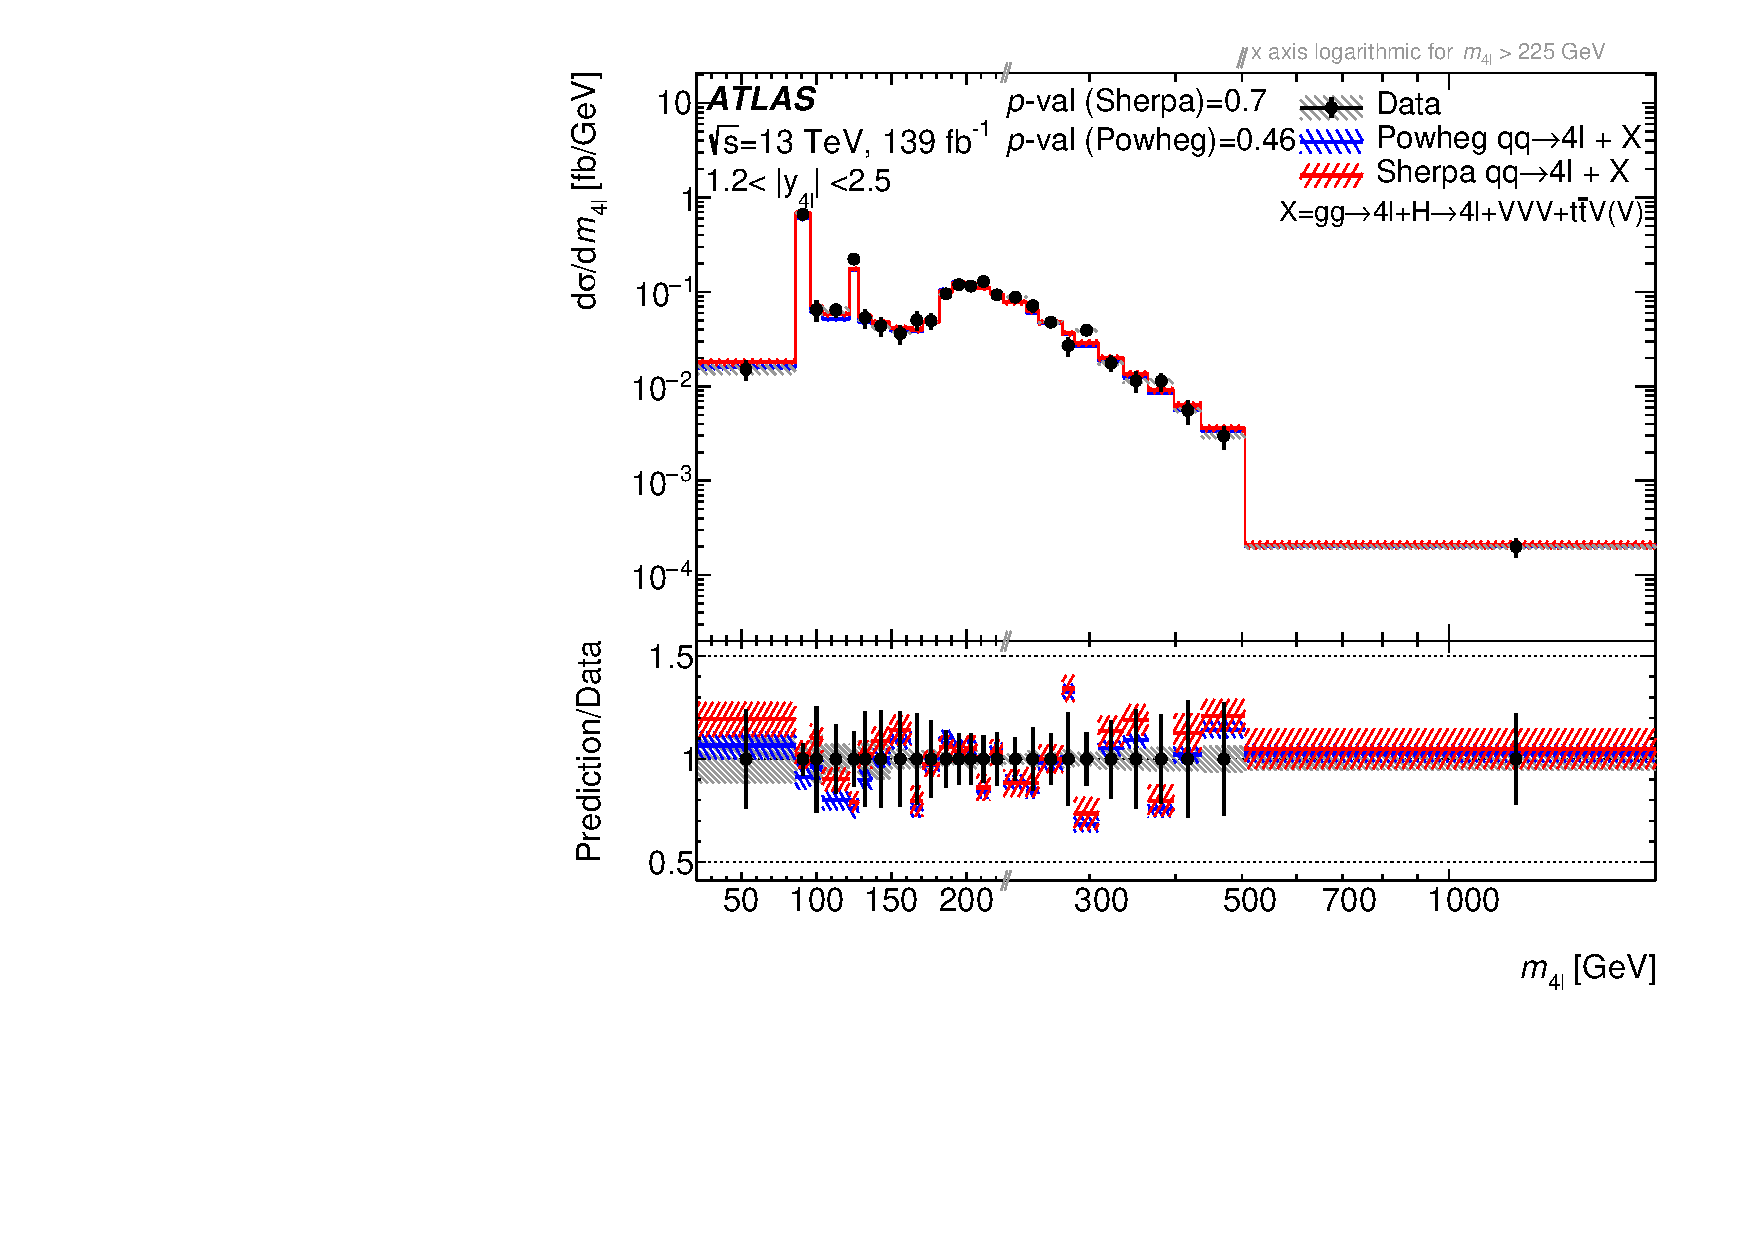
\includegraphics[width=.99\linewidth]{Figures/m4l/UnfoldedResults/linlog_Unfolded_Data_m4l_y4l1dot2-2dot5.pdf}  \caption{1.2 < \yFourL{} < 2.5}\label{fig:sub-fifth}
    \end{subfigure}
    \caption{Differential cross-section as a function of \mFourL{} in slices of \yFourL{}. The measured data (black points) are  compared with the SM prediction using either \SHERPA{} (red, with red hashed band for the uncertainty) or \POWHEG{} + \pythia{} (blue, with blue hashed band for the uncertainty) to model the \qqFourL{} contribution. The error bars on the data points give the total uncertainty and the grey hashed band gives the systematic uncertainty. \Pvalue{} The  lower panel shows the ratio of the SM predictions to the data.}
    \label{fig:m4l_y4l}
\end{figure}

%% m4l vs flavour
\begin{figure}[htb!]
    \begin{subfigure}{.49\textwidth}\centering
      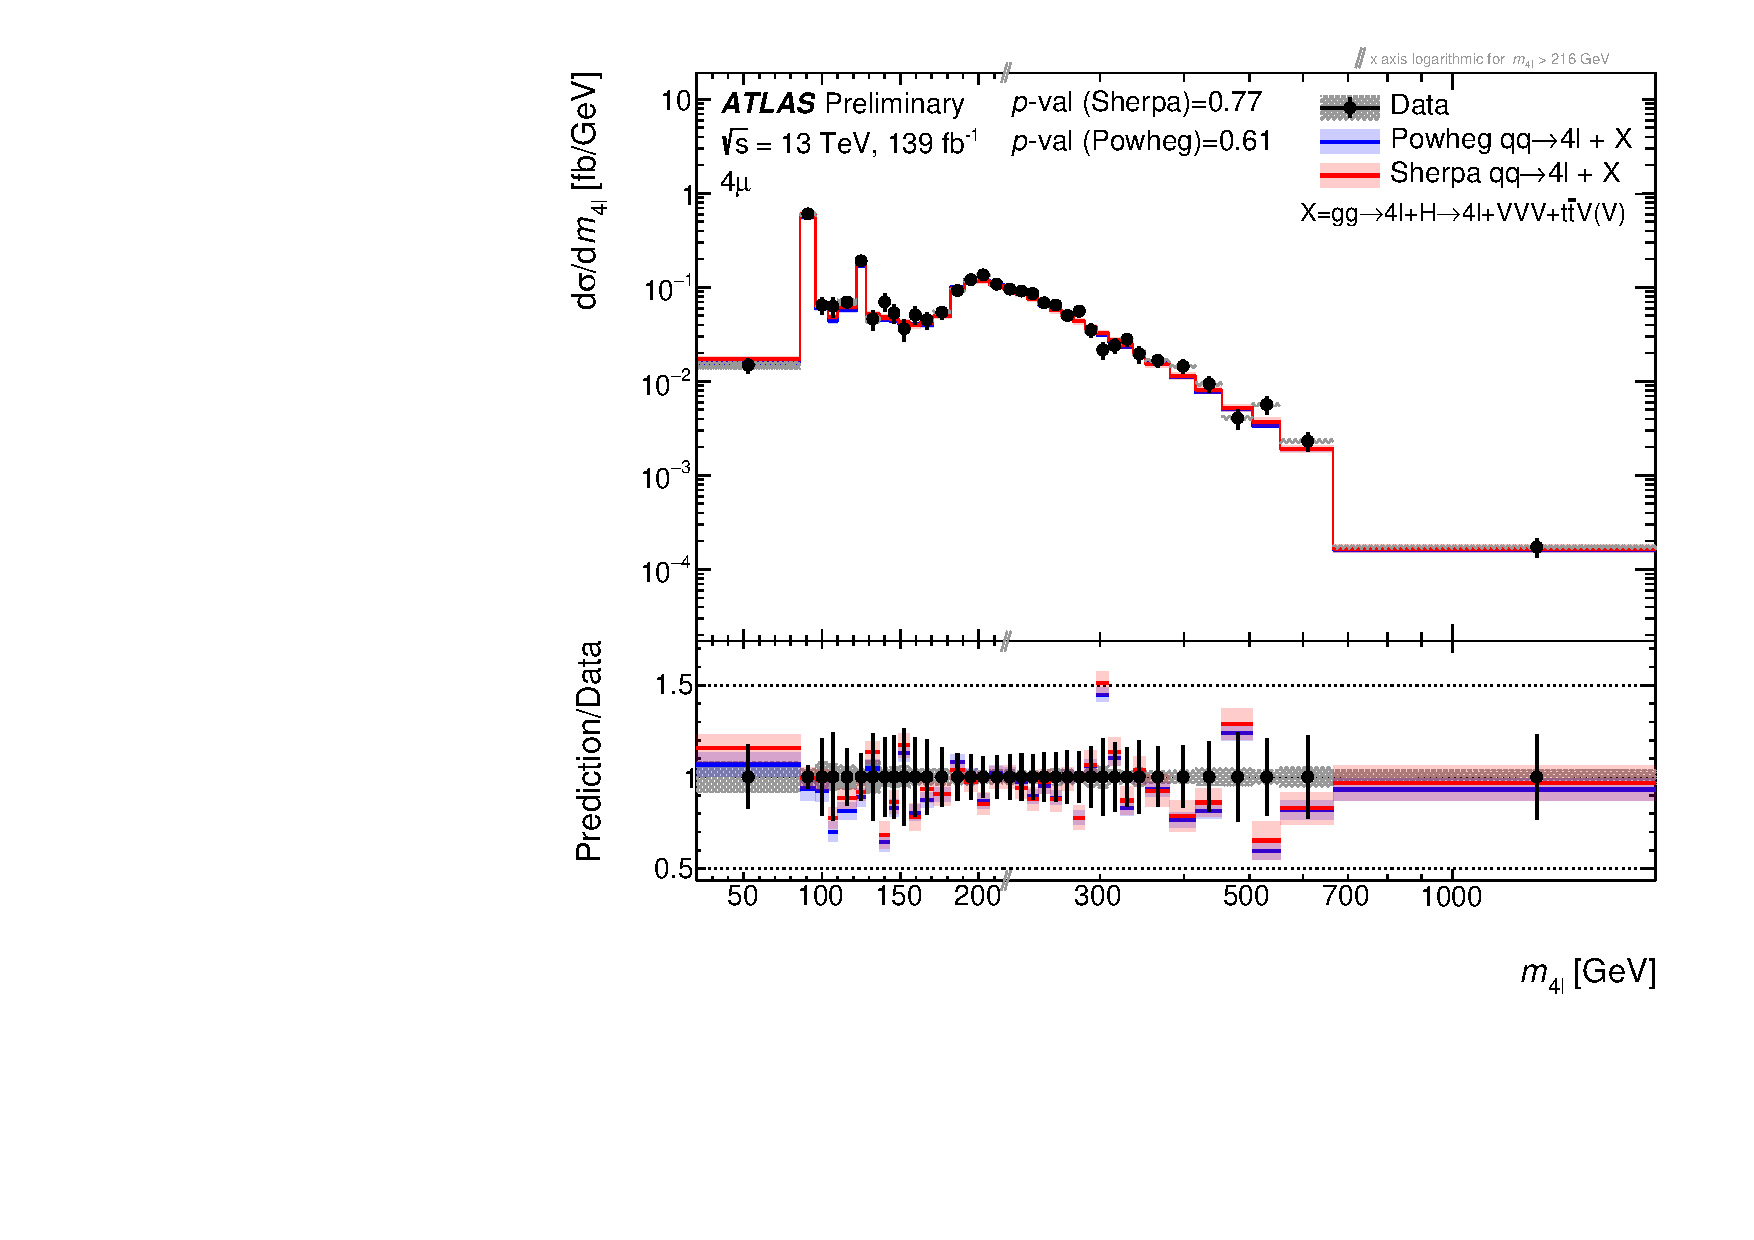
\includegraphics[width=.99\linewidth]{Figures/m4l/UnfoldedResults/linlog_Unfolded_Data_m4l_event_type4mu.pdf}\caption{$4\mu$ channel}\label{fig:sub-first}
    \end{subfigure}
    \begin{subfigure}{.49\textwidth}\centering
      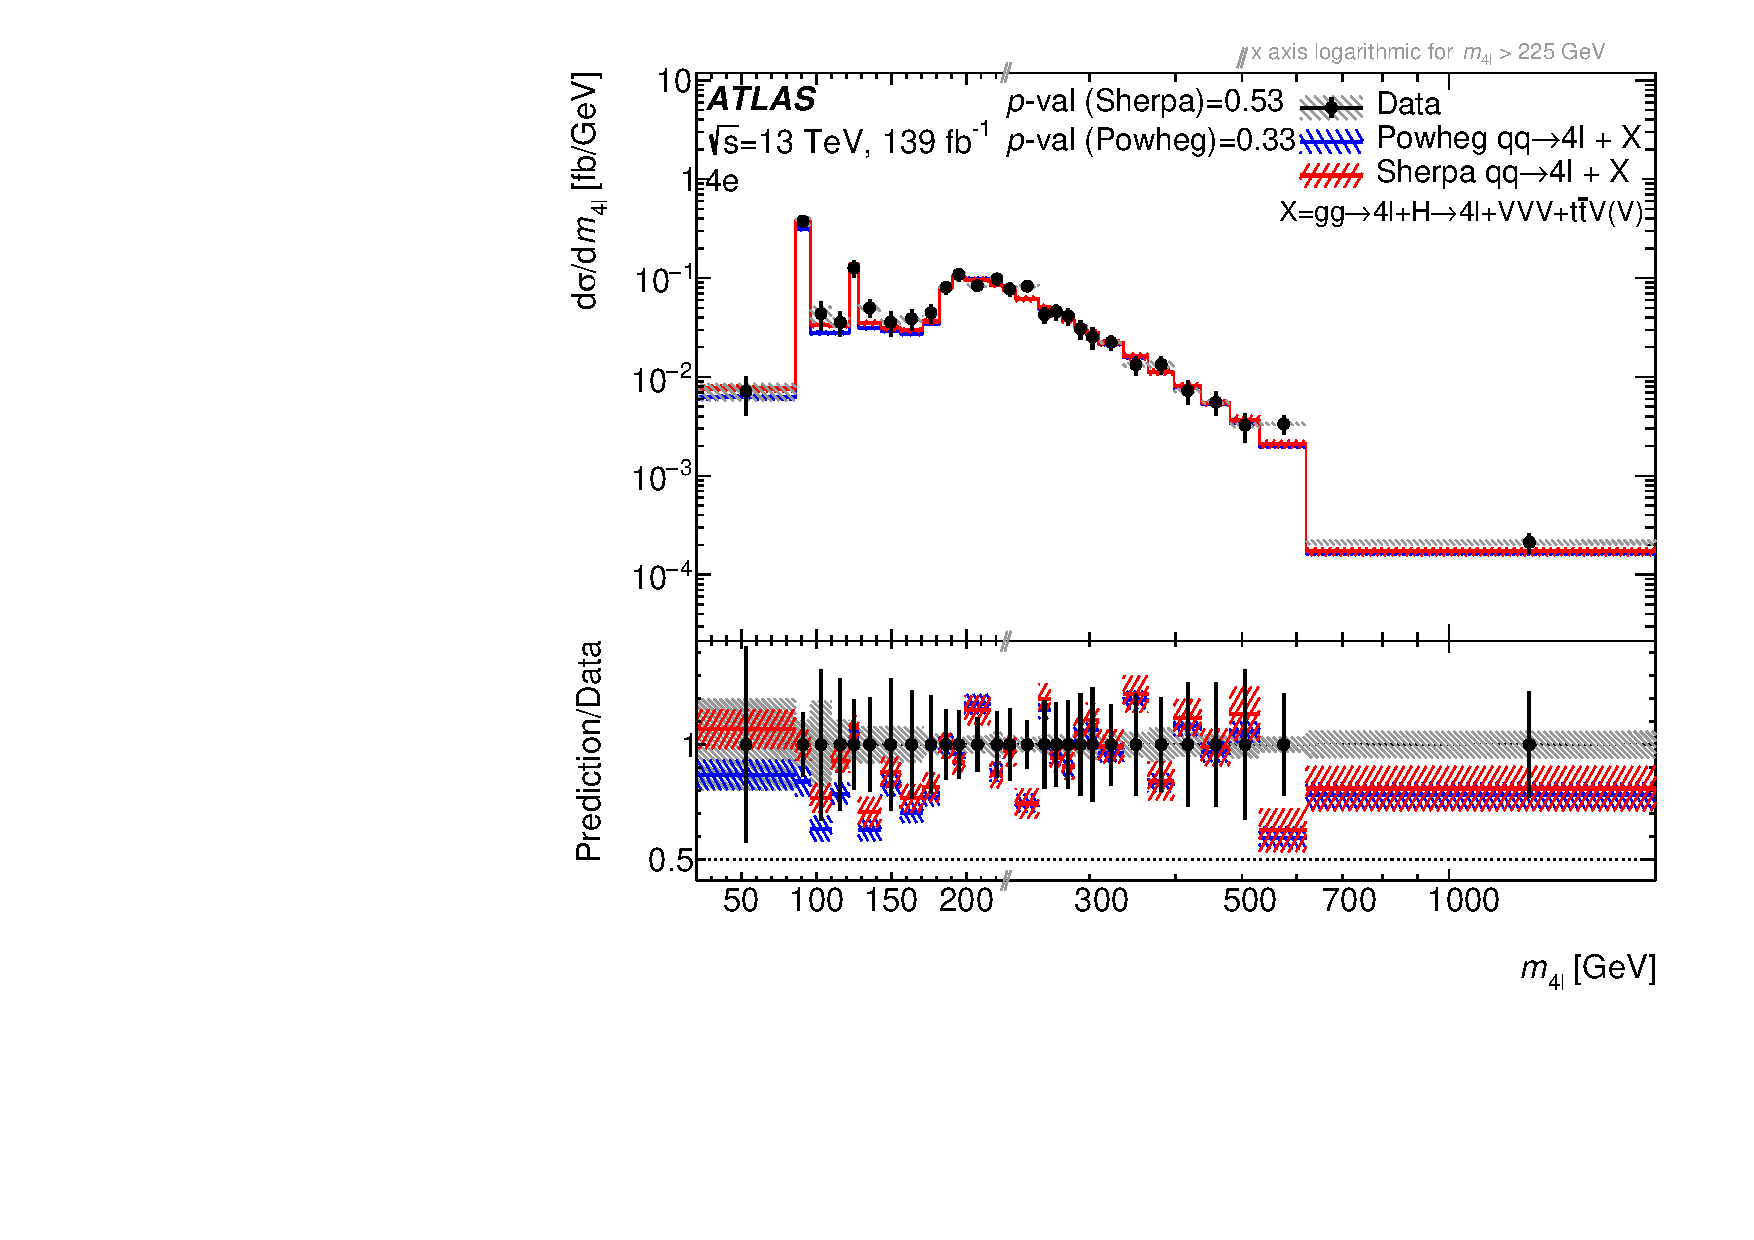
\includegraphics[width=.99\linewidth]{Figures/m4l/UnfoldedResults/linlog_Unfolded_Data_m4l_event_type4e.pdf} \caption{$4e$ channel}\label{fig:sub-second}
    \end{subfigure}
    \begin{subfigure}{.49\textwidth}\centering
      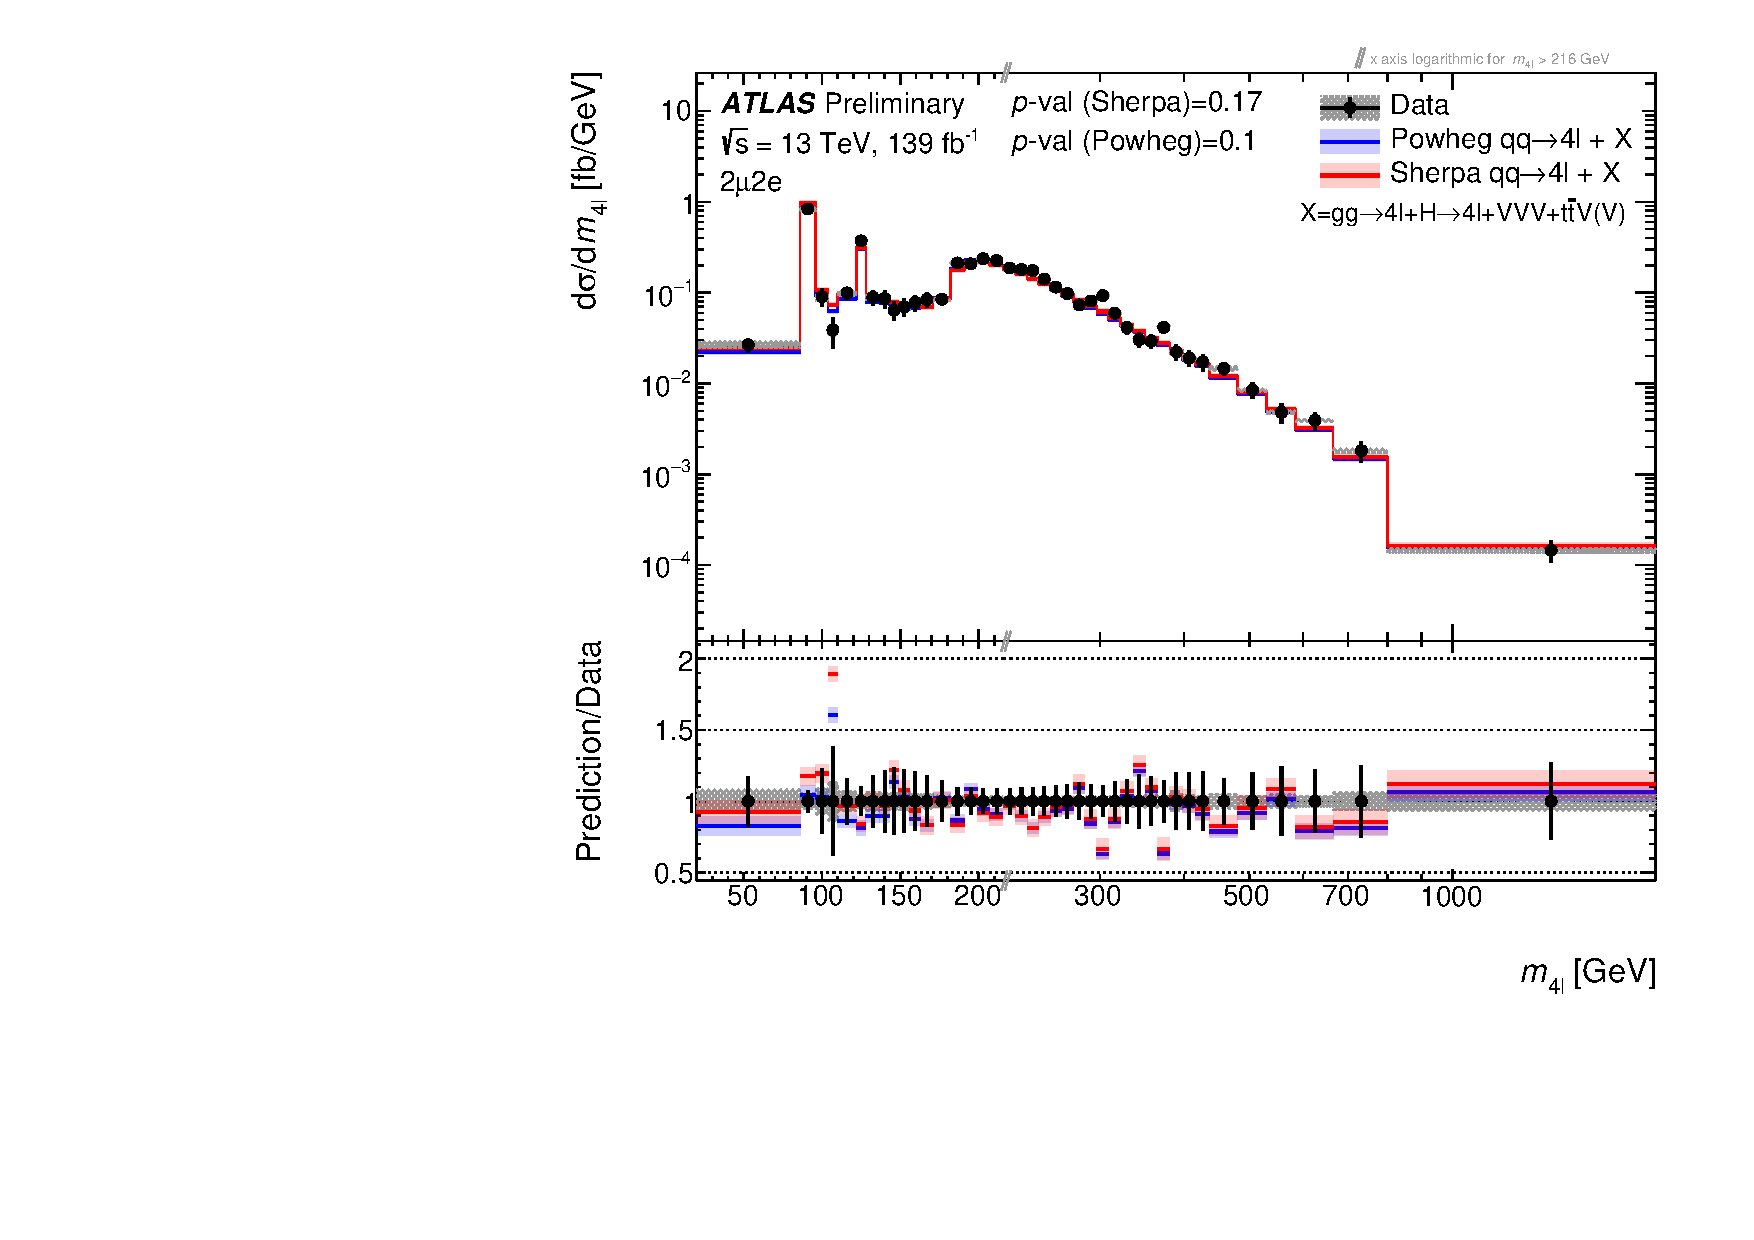
\includegraphics[width=.99\linewidth]{Figures/m4l/UnfoldedResults/linlog_Unfolded_Data_m4l_event_type2mu2e.pdf}  \caption{$2e2\mu$ channel}\label{fig:sub-third}
    \end{subfigure}
    \caption{Differential cross-section as a function of \mFourL{} for each lepton flavour channel. The measured data (black points)  are compared with the SM prediction using either \SHERPA{} (red, with red hashed band for the uncertainty) or \POWHEG{} + \pythia{} (blue, with blue hashed band for the uncertainty) to model the \qqFourL{} contribution. The error bars on the data points give the total uncertainty and the grey hashed band gives the systematic uncertainty. \Pvalue{} The lower panel shows the ratio of the SM predictions to the data.  The $x$-axis is on a linear scale until $\mFourL = 225$~\GeV, where it switches to a logarithmic scale.}
    \label{fig:m4l_flavour}
\end{figure}

%% m12 vs m4l
\begin{figure}[htb!]
    \begin{subfigure}{.49\textwidth}\centering
      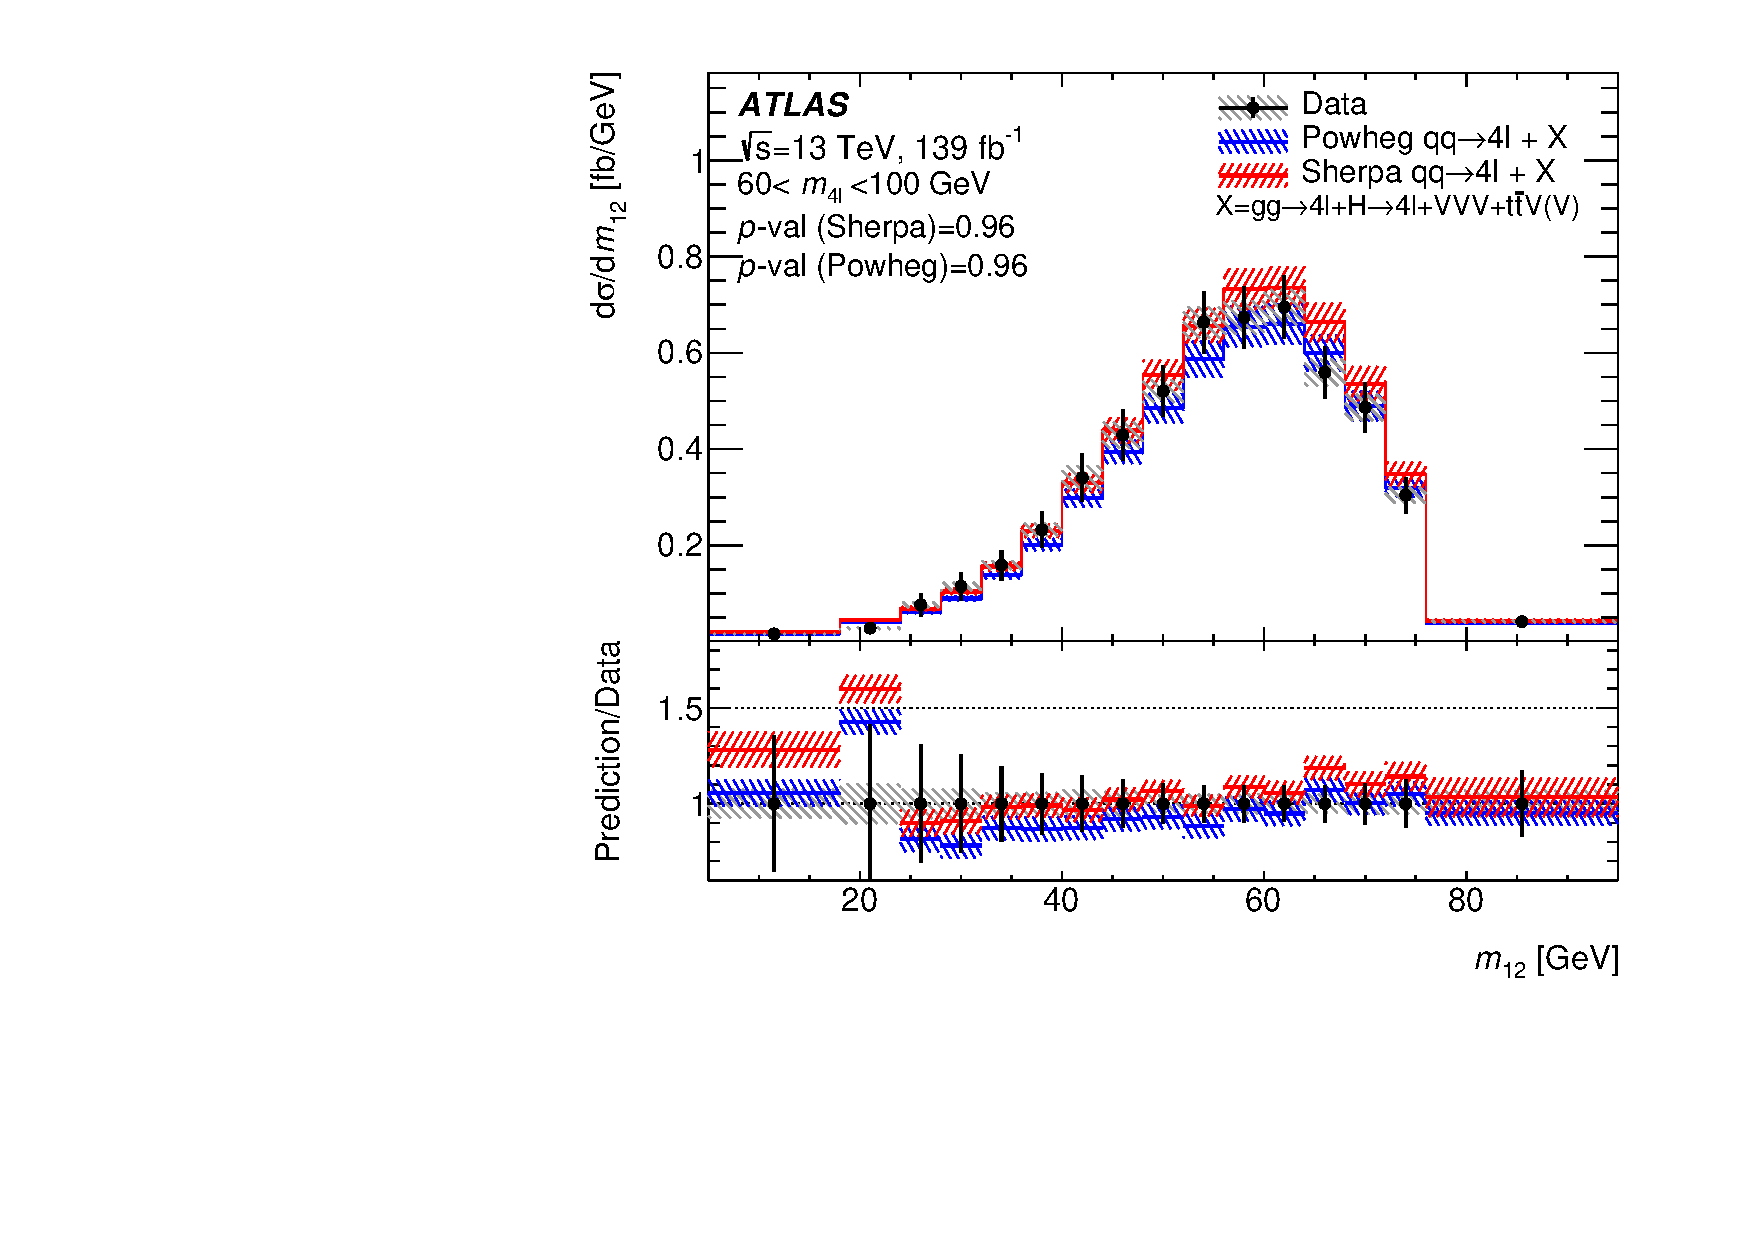
\includegraphics[width=.99\linewidth]{Figures/m4l/UnfoldedResults/linY_Unfolded_Data_m12_m4l60-100.pdf}  
      \caption{\ZFourL \ region}
      \label{fig:sub-first}
    \end{subfigure}
    \begin{subfigure}{.49\textwidth}\centering
      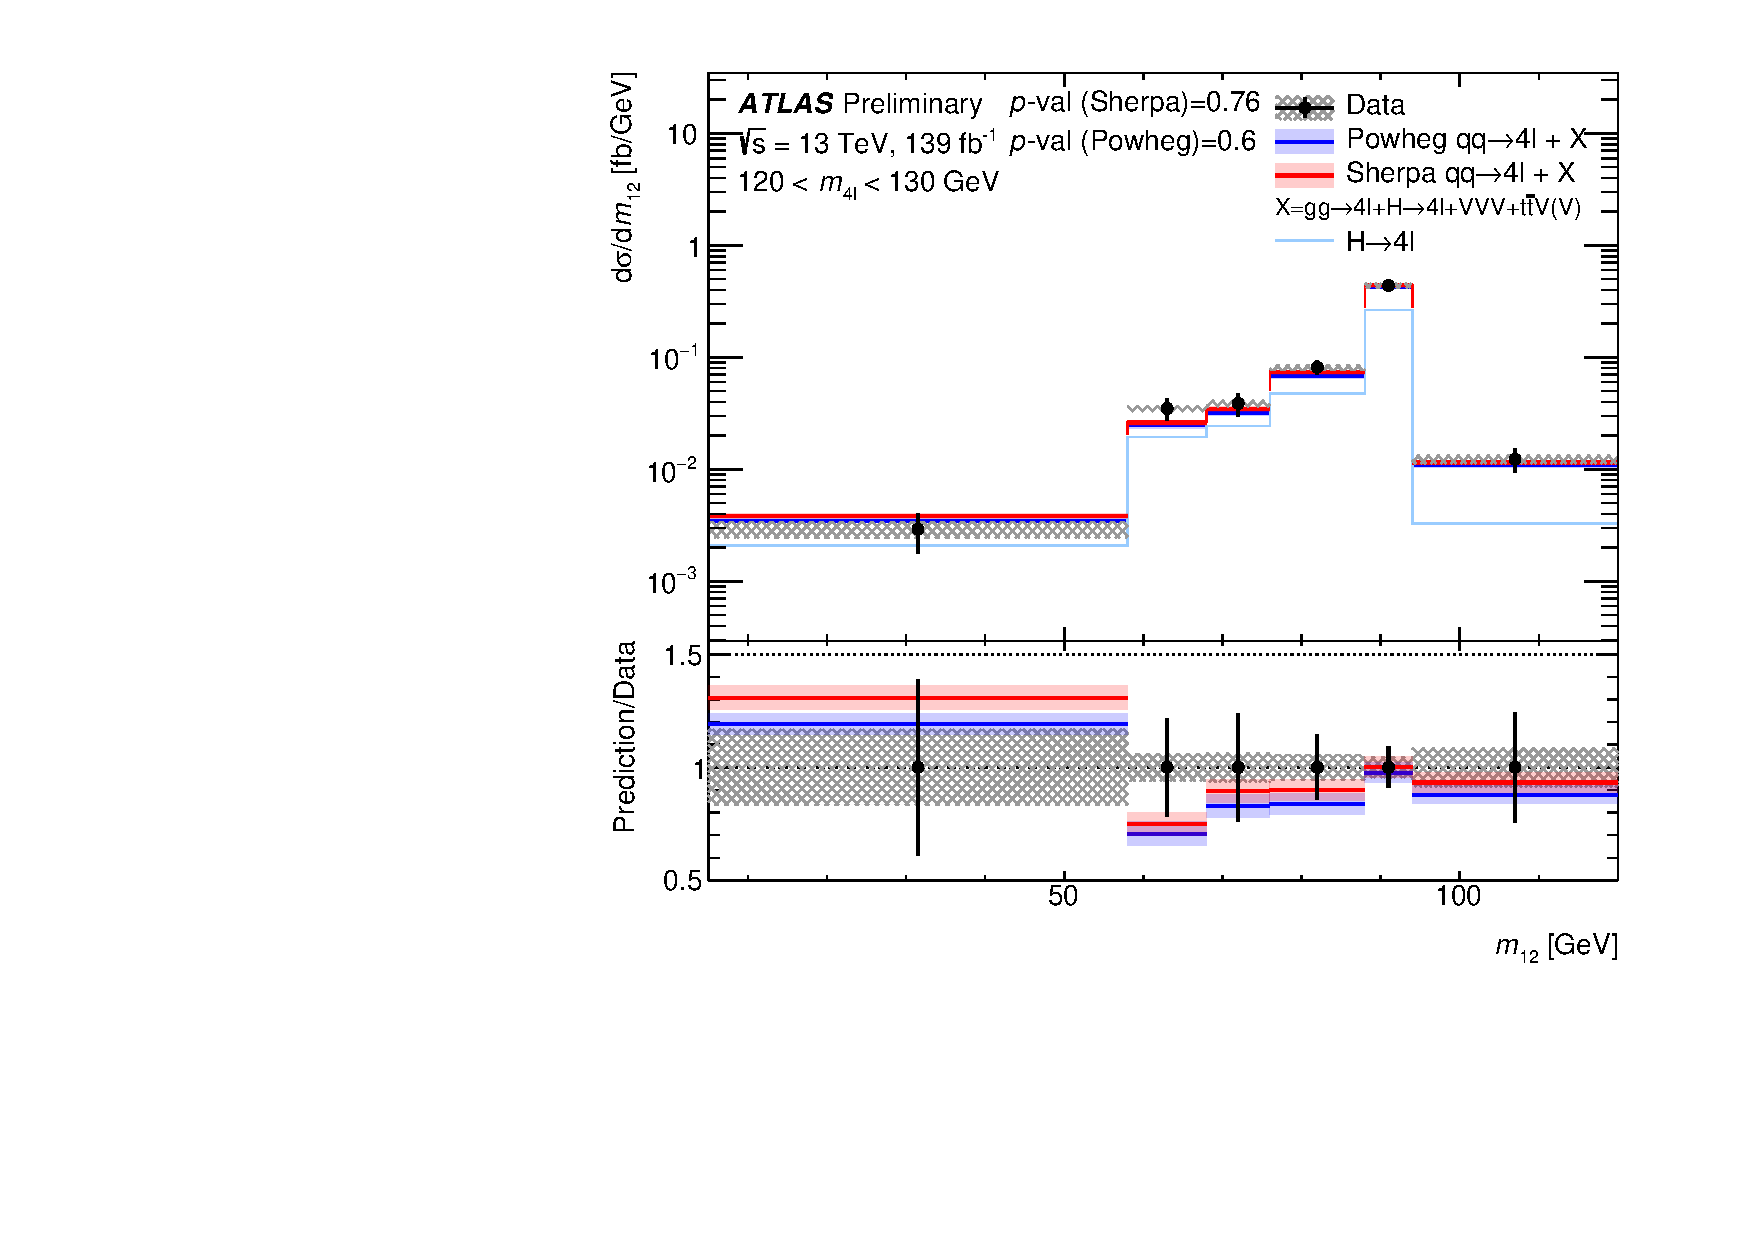
\includegraphics[width=.99\linewidth]{Figures/m4l/UnfoldedResults/higgs_Unfolded_Data_m12_m4l120-130.pdf}  
      \caption{\HFourL \ region}
      \label{fig:sub-second}
    \end{subfigure}
    \begin{subfigure}{.49\textwidth}
      \centering
      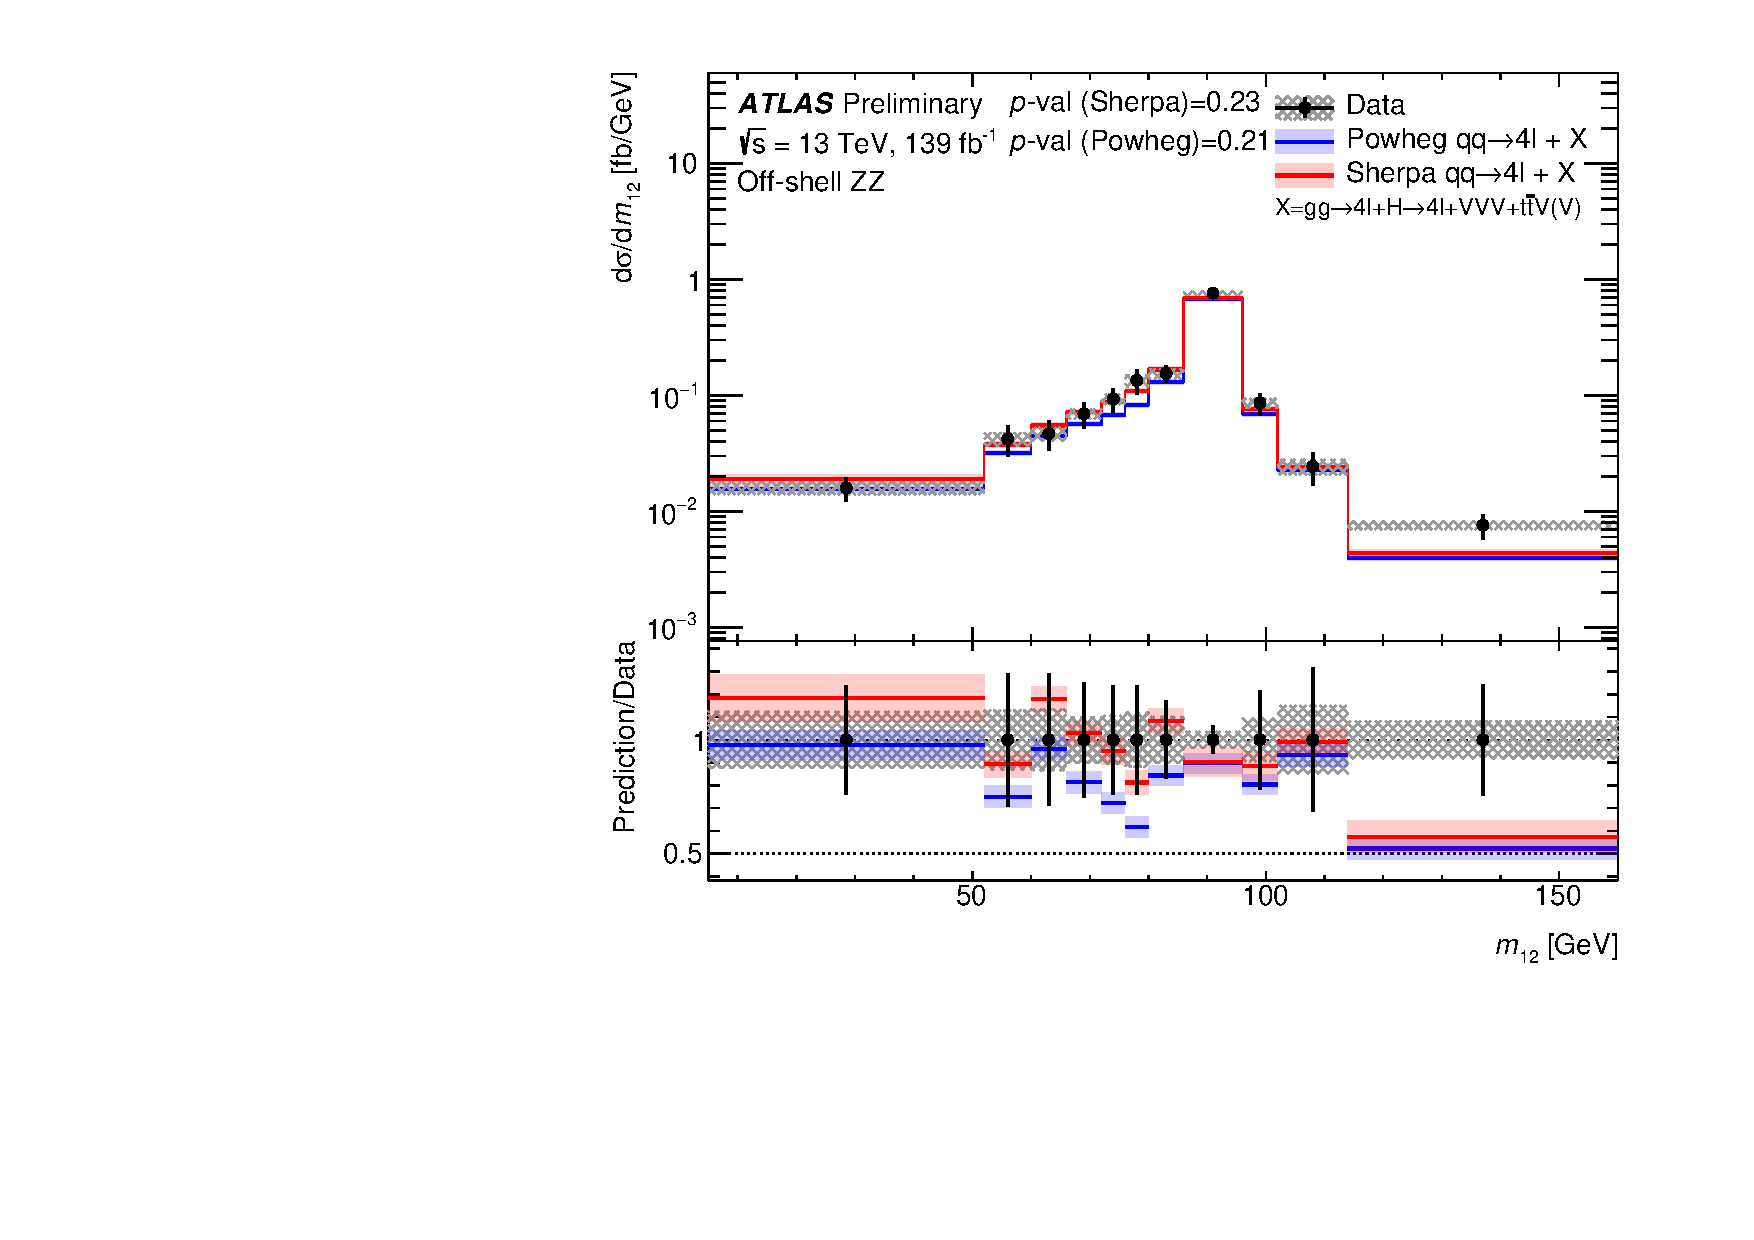
\includegraphics[width=.99\linewidth]{Figures/m4l/UnfoldedResults/Unfolded_Data_m12_m4loffshell.pdf}  
      \caption{Off-shell $\Z\Z$ region}
      \label{fig:sub-third}
    \end{subfigure}
    \begin{subfigure}{.49\textwidth}
      \centering
      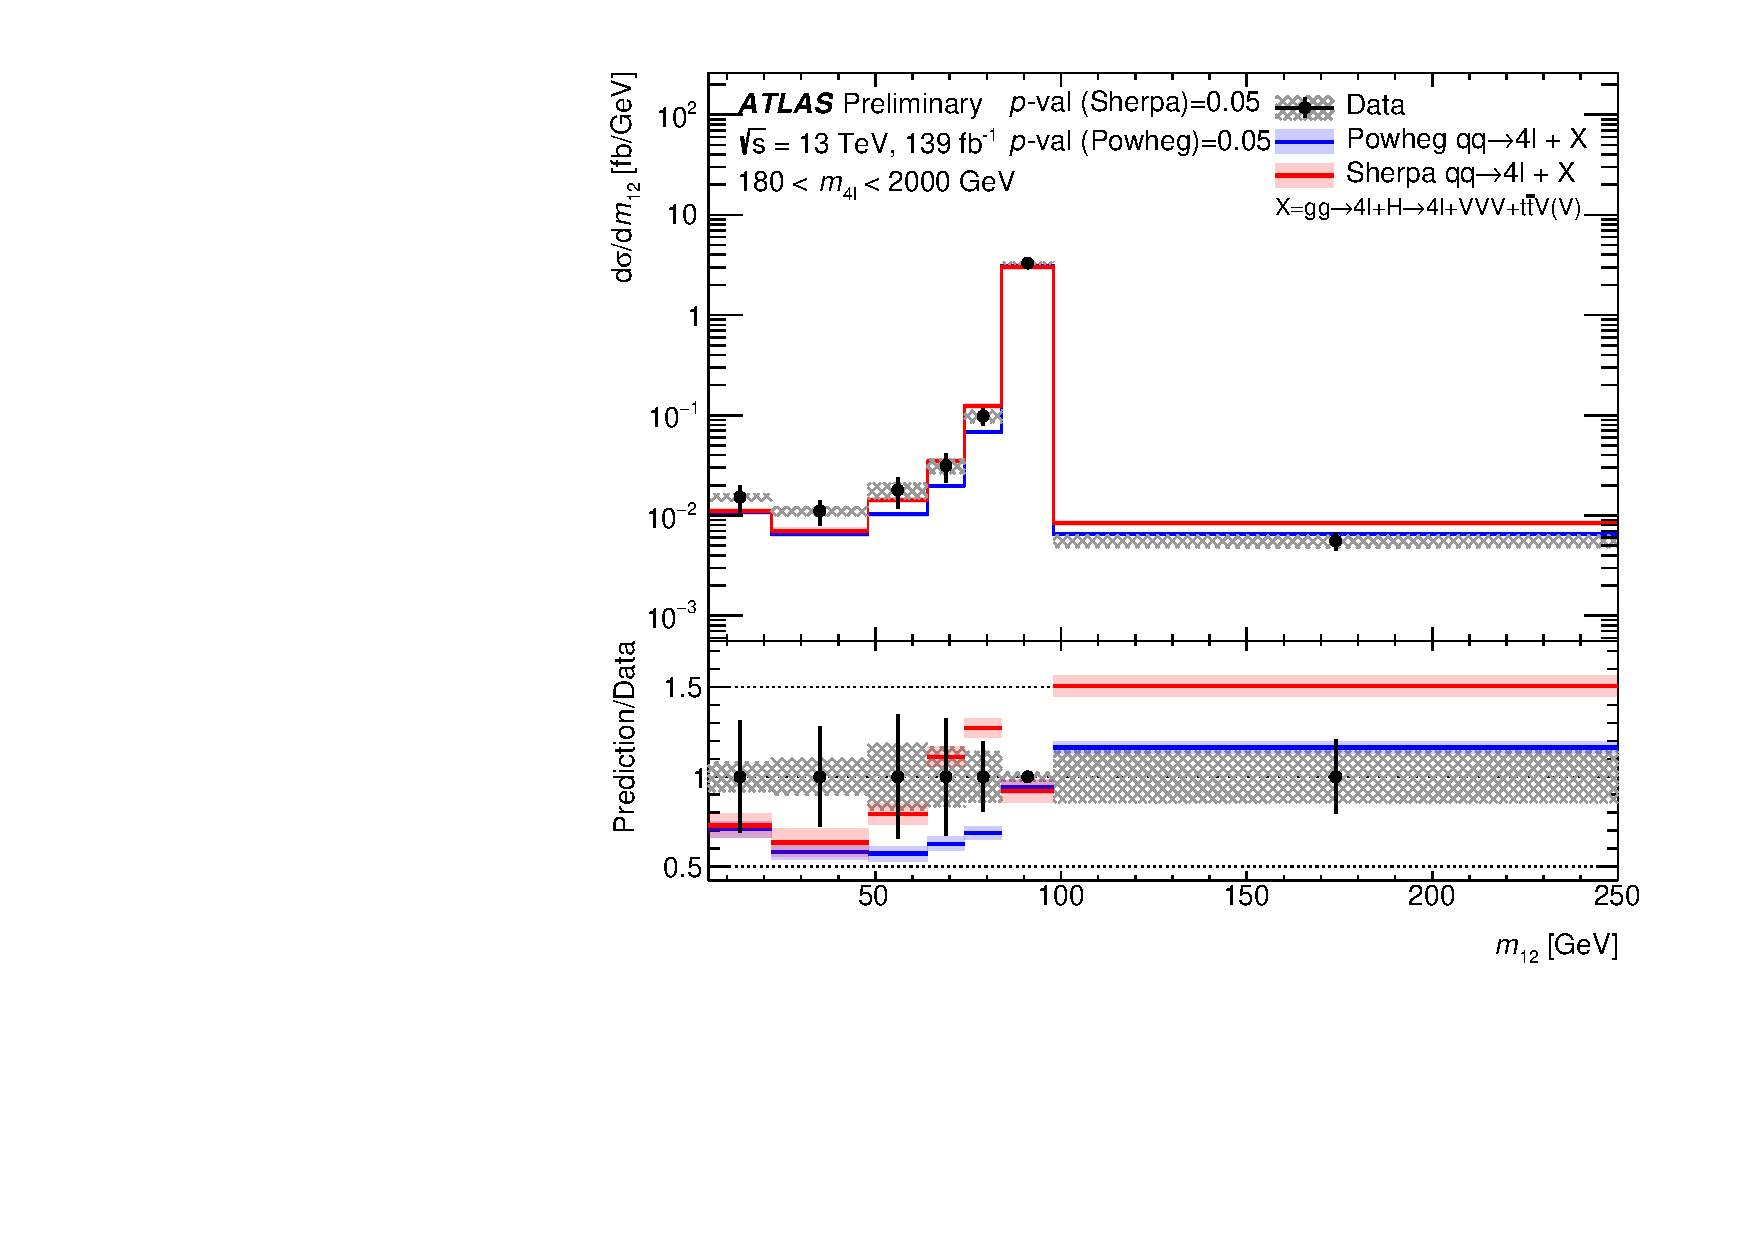
\includegraphics[width=.99\linewidth]{Figures/m4l/UnfoldedResults/Unfolded_Data_m12_m4l180-2000.pdf}  
      \caption{On-shell $\Z\Z$ region}
      \label{fig:sub-fourth}
    \end{subfigure}
    \caption{Differential cross-section as a function of \mZOne{} in the four
        \mFourL{} regions. The measured data (black points) are  compared with the SM prediction using either \SHERPA{} (red, with red hashed band for the uncertainty) or \POWHEG{} + \pythia{} (blue, with blue hashed band for the uncertainty) to model the \qqFourL{} contribution. In (b) the contribution from Higgs production is shown in addition to the total SM prediction. The error bars on the data points give the total uncertainty and the grey hashed band gives the systematic uncertainty. \Pvalue{} The  lower panel shows the ratio of the SM predictions to the data.}
    \label{fig:m12_m4l}
\end{figure}

%% m34 vs m4l
\begin{figure}[htb!]
    \begin{subfigure}{.49\textwidth}\centering
      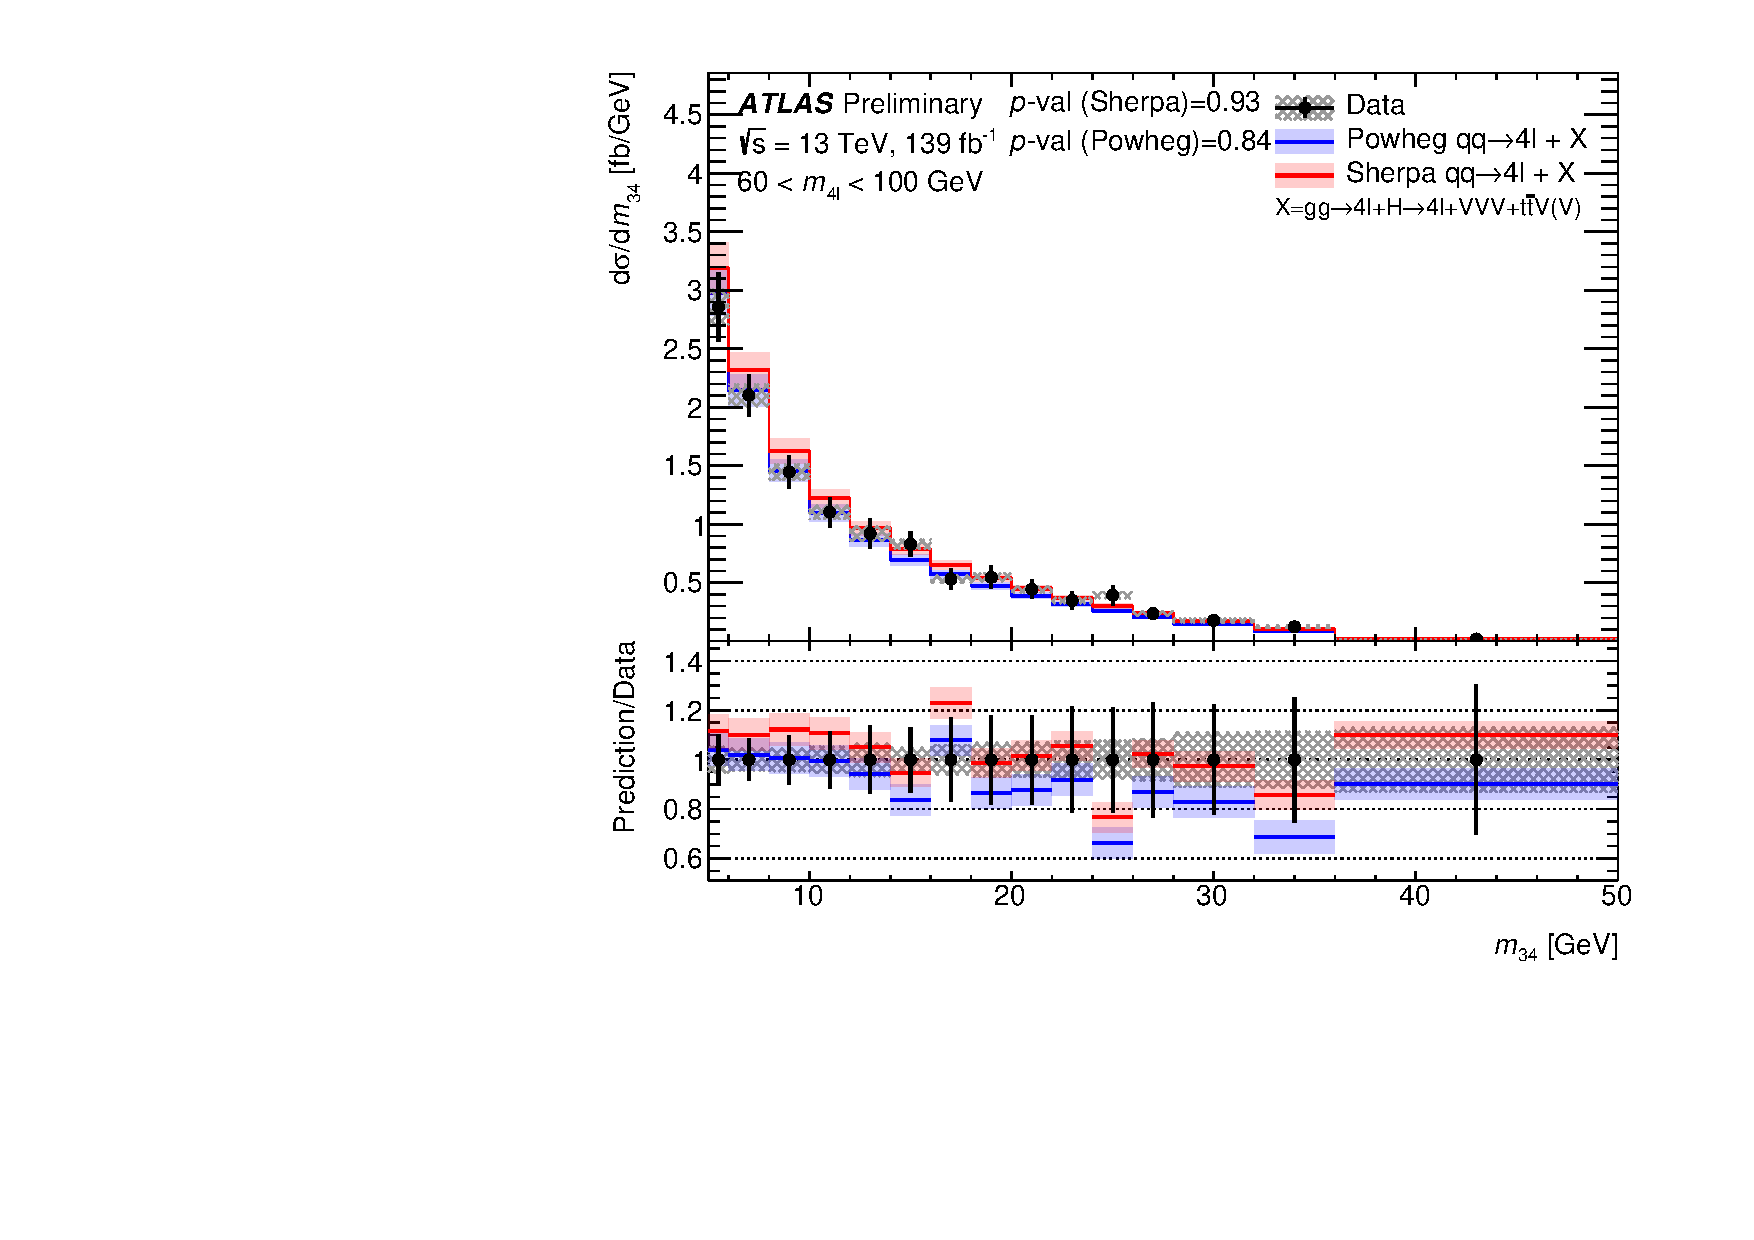
\includegraphics[width=.99\linewidth]{Figures/m4l/UnfoldedResults/linY_Unfolded_Data_m34_m4l60-100.pdf}\caption{\ZFourL \ region}\label{fig:sub-first}
    \end{subfigure}
    \begin{subfigure}{.49\textwidth}\centering
      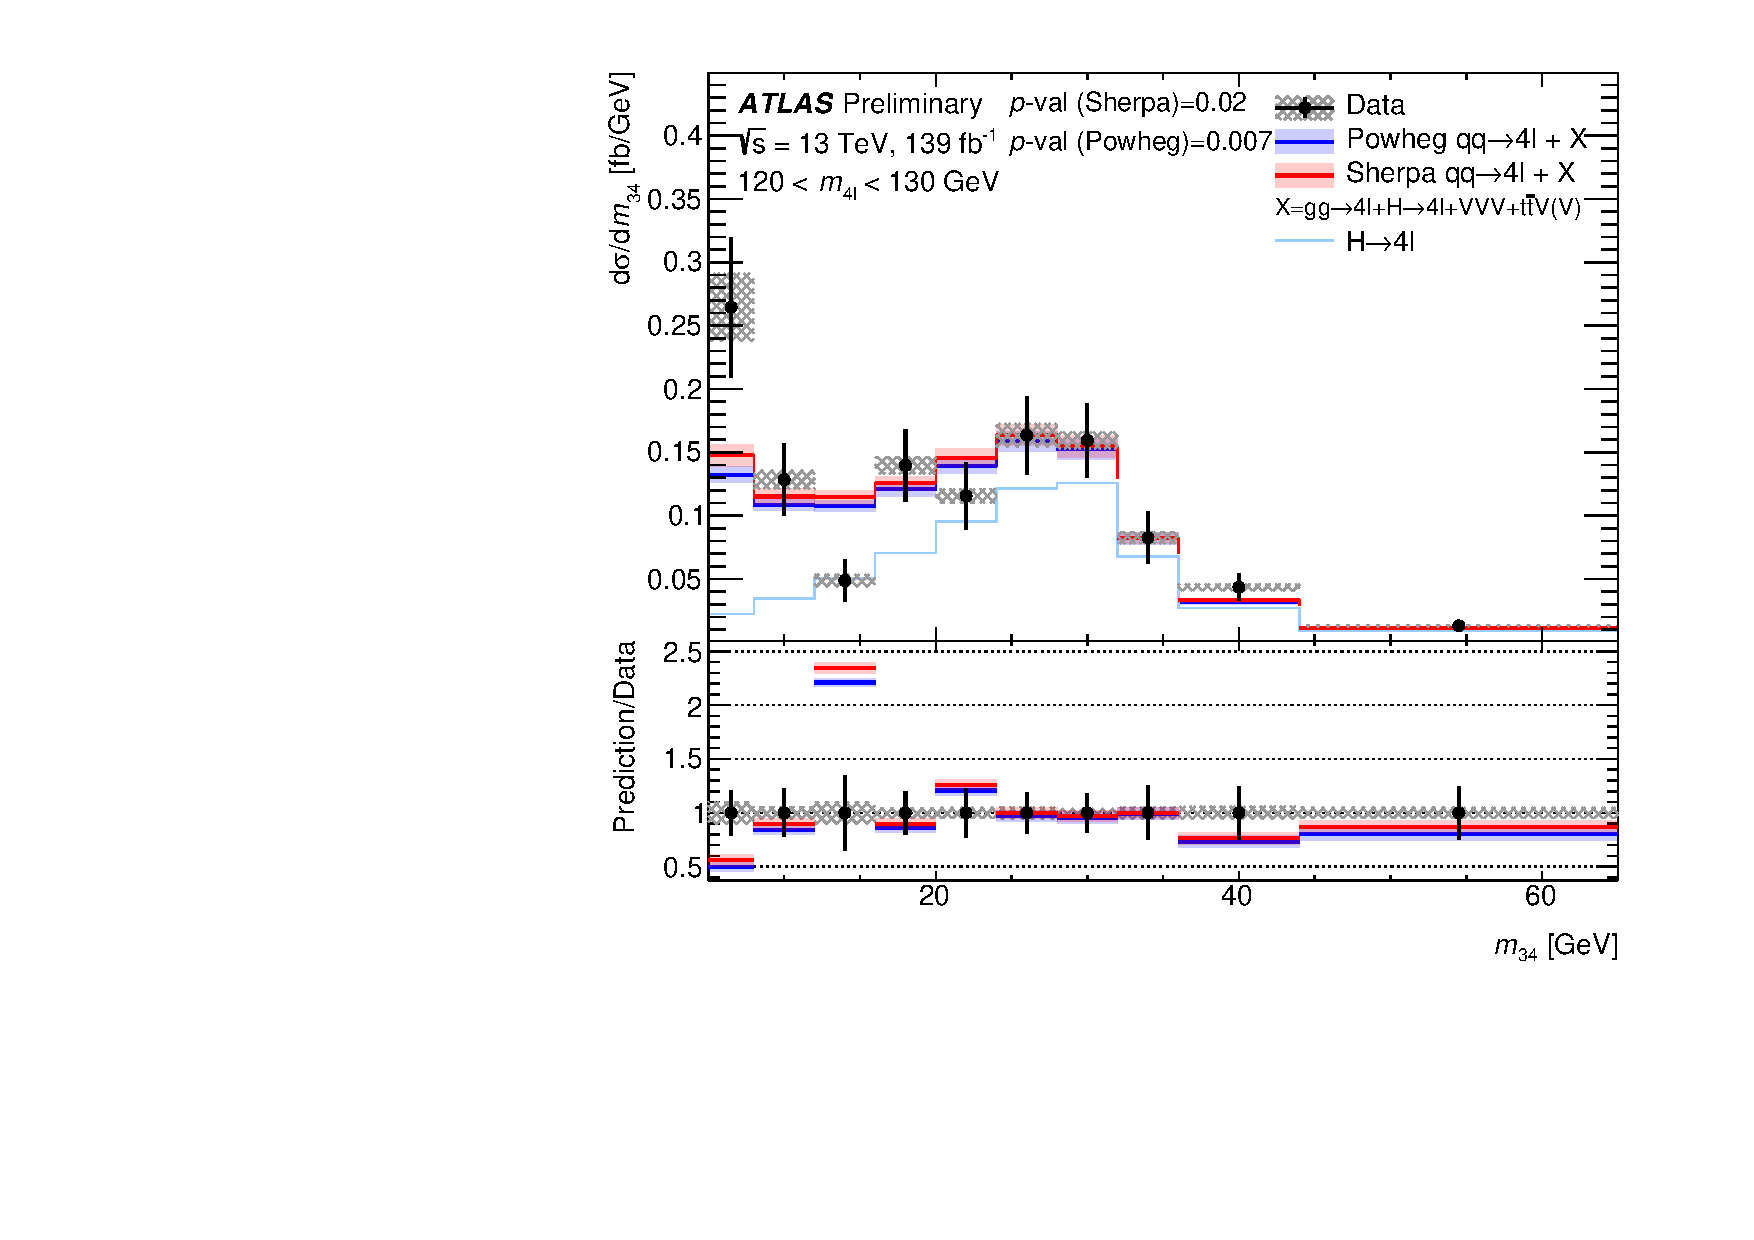
\includegraphics[width=.99\linewidth]{Figures/m4l/UnfoldedResults/higgs_linY_Unfolded_Data_m34_m4l120-130.pdf} \caption{\HFourL \ region}\label{fig:sub-second}
    \end{subfigure}
    \begin{subfigure}{.49\textwidth}\centering
      \includegraphics[width=.99\linewidth]{Figures/m4l/UnfoldedResults/linY_Unfolded_Data_m34_m4loffshell.pdf}  \caption{Off-shell $\Z\Z$ region}\label{fig:sub-third}
    \end{subfigure}
    \begin{subfigure}{.49\textwidth}\centering
      \includegraphics[width=.99\linewidth]{Figures/m4l/UnfoldedResults/Unfolded_Data_m34_m4l180-2000.pdf}  \caption{On-shell $\Z\Z$ region}\label{fig:sub-fourth}
    \end{subfigure}
    \caption{Differential cross-section as a function of \mZTwo{} in the four
        \mFourL{} regions. The measured data (black points) are  compared with the SM prediction using either \SHERPA{} (red, with red hashed band for the uncertainty) or \POWHEG{} + \pythia{} (blue, with blue hashed band for the uncertainty) to model the \qqFourL{} contribution. In (b) the contribution from Higgs production is shown in addition to the total SM prediction. The error bars on the data points give the total uncertainty and the grey hashed band gives the systematic uncertainty. \Pvalue{} The  lower panel shows the ratio of the SM predictions to the data.}
    \label{fig:m34_m4l}
\end{figure}

%% pt12 vs m4l
\begin{figure}[htb!]
    \begin{subfigure}{.49\textwidth}\centering
      \includegraphics[width=.99\linewidth]{Figures/m4l/UnfoldedResults/linlog_Unfolded_Data_pt12_m4l60-100.pdf}\caption{\ZFourL \ region}\label{fig:sub-first}
    \end{subfigure}
    \begin{subfigure}{.49\textwidth}\centering
      \includegraphics[width=.99\linewidth]{Figures/m4l/UnfoldedResults/linlog_Unfolded_Data_pt12_m4l120-130.pdf} \caption{\HFourL \ region}\label{fig:sub-second}
    \end{subfigure}
    \begin{subfigure}{.49\textwidth}\centering
      \includegraphics[width=.99\linewidth]{Figures/m4l/UnfoldedResults/linlog_Unfolded_Data_pt12_m4loffshell.pdf}  \caption{Off-shell $\Z\Z$ region}\label{fig:sub-third}
    \end{subfigure}
    \begin{subfigure}{.49\textwidth}\centering
      \includegraphics[width=.99\linewidth]{Figures/m4l/UnfoldedResults/linlog_Unfolded_Data_pt12_m4l180-2000.pdf}  \caption{On-shell $\Z\Z$ region}\label{fig:sub-fourth}
    \end{subfigure}
    \caption{Differential cross-section as a function of \ptZOne{} in the four
        \mFourL{} regions. The measured data (black points) are  compared with the SM prediction using either \SHERPA{} (red, with red hashed band for the uncertainty) or \POWHEG{} + \pythia{} (blue, with blue hashed band for the uncertainty) to model the \qqFourL{} contribution. In (b) the contribution from Higgs production is shown in addition to the total SM prediction. The error bars on the data points give the total uncertainty and the grey hashed band gives the systematic uncertainty. \Pvalue{} The  lower panel shows the ratio of the SM predictions to the data.}
    \label{fig:pt12_m4l}
\end{figure}

%% pt34 vs m4l
\begin{figure}[htb!]
    \begin{subfigure}{.49\textwidth}\centering
      \includegraphics[width=.99\linewidth]{Figures/m4l/UnfoldedResults/linlog_Unfolded_Data_pt34_m4l60-100.pdf}\caption{\ZFourL \ region}\label{fig:sub-first}
    \end{subfigure}
    \begin{subfigure}{.49\textwidth}\centering
      \includegraphics[width=.99\linewidth]{Figures/m4l/UnfoldedResults/linlog_Unfolded_Data_pt34_m4l120-130.pdf} \caption{\HFourL \ region}\label{fig:sub-second}
    \end{subfigure}
    \begin{subfigure}{.49\textwidth}\centering
      \includegraphics[width=.99\linewidth]{Figures/m4l/UnfoldedResults/linlog_Unfolded_Data_pt34_m4loffshell.pdf}  \caption{Off-shell $\Z\Z$ region}\label{fig:sub-third}
    \end{subfigure}
    \begin{subfigure}{.49\textwidth}\centering
      \includegraphics[width=.99\linewidth]{Figures/m4l/UnfoldedResults/linlog_Unfolded_Data_pt34_m4l180-2000.pdf}  \caption{On-shell $\Z\Z$ region}\label{fig:sub-fourth}
    \end{subfigure}
    \caption{Differential cross-section as a function of \ptZTwo{} in the four
        \mFourL{} regions. The measured data (black points) are  compared with the SM prediction using either \SHERPA{} (red, with red hashed band for the uncertainty) or \POWHEG{} + \pythia{} (blue, with blue hashed band for the uncertainty) to model the \qqFourL{} contribution. The error bars on the data points give the total uncertainty and the grey hashed band gives the systematic uncertainty. \Pvalue{} The  lower panel shows the ratio of the SM predictions to the data.}
    \label{fig:pt23_m4l}
\end{figure}

%% cosThetaStar1 vs m4l
\begin{figure}[htb!]
    \begin{subfigure}{.49\textwidth}\centering
      \includegraphics[width=.99\linewidth]{Figures/m4l/UnfoldedResults/linY_Unfolded_Data_cosThetaStar1_m4l60-100.pdf}\caption{\ZFourL \ region}\label{fig:sub-first}
    \end{subfigure}
    \begin{subfigure}{.49\textwidth}\centering
      \includegraphics[width=.99\linewidth]{Figures/m4l/UnfoldedResults/linY_Unfolded_Data_cosThetaStar1_m4l120-130.pdf} \caption{\HFourL \ region}\label{fig:sub-second}
    \end{subfigure}
    \begin{subfigure}{.49\textwidth}\centering
      \includegraphics[width=.99\linewidth]{Figures/m4l/UnfoldedResults/linY_Unfolded_Data_cosThetaStar1_m4loffshell.pdf}  \caption{Off-shell $\Z\Z$ region}\label{fig:sub-third}
    \end{subfigure}
    \begin{subfigure}{.49\textwidth}\centering
      \includegraphics[width=.99\linewidth]{Figures/m4l/UnfoldedResults/linY_Unfolded_Data_cosThetaStar1_m4l180-2000.pdf}  \caption{On-shell $\Z\Z$ region}\label{fig:sub-fourth}
    \end{subfigure}
    \caption{Differential cross-section as a function of \CTSOneTwo{} in the four
        \mFourL{} regions. The measured data (black points) are  compared with the SM prediction using either \SHERPA{} (red, with red hashed band for the uncertainty) or \POWHEG{} + \pythia{} (blue, with blue hashed band for the uncertainty) to model the \qqFourL{} contribution. The error bars on the data points give the total uncertainty and the grey hashed band gives the systematic uncertainty. \Pvalue{} The  lower panel shows the ratio of the SM predictions to the data.}
    \label{fig:cts12_m4l}
\end{figure}

%% cosThetaStar3 vs m4l
\begin{figure}[htb!]
    \begin{subfigure}{.49\textwidth}\centering
      \includegraphics[width=.99\linewidth]{Figures/m4l/UnfoldedResults/linY_Unfolded_Data_cosThetaStar3_m4l60-100.pdf}\caption{\ZFourL \ region}\label{fig:sub-first}
    \end{subfigure}
    \begin{subfigure}{.49\textwidth}\centering
      \includegraphics[width=.99\linewidth]{Figures/m4l/UnfoldedResults/linY_Unfolded_Data_cosThetaStar3_m4l120-130.pdf} \caption{\HFourL \ region}\label{fig:sub-second}
    \end{subfigure}
    \begin{subfigure}{.49\textwidth}\centering
      \includegraphics[width=.99\linewidth]{Figures/m4l/UnfoldedResults/linY_Unfolded_Data_cosThetaStar3_m4loffshell.pdf}  \caption{Off-shell $\Z\Z$ region}\label{fig:sub-third}
    \end{subfigure}
    \begin{subfigure}{.49\textwidth}\centering
      \includegraphics[width=.99\linewidth]{Figures/m4l/UnfoldedResults/linY_Unfolded_Data_cosThetaStar3_m4l180-2000.pdf}  \caption{On-shell $\Z\Z$ region}\label{fig:sub-fourth}
    \end{subfigure}
    \caption{Differential cross-section as a function of \CTSThreeFour{} in the four
        \mFourL{} regions. The measured data (black points) are  compared with the SM prediction using either \SHERPA{} (red, with red hashed band for the uncertainty) or \POWHEG{} + \pythia{} (blue, with blue hashed band for the uncertainty) to model the \qqFourL{} contribution. The error bars on the data points give the total uncertainty and the grey hashed band gives the systematic uncertainty. \Pvalue{} The  lower panel shows the ratio of the SM predictions to the data.}
    \label{fig:cts34_m4l}
\end{figure}

%% deltaPhiLeptons vs m4l
\begin{figure}[htb!]
    \begin{subfigure}{.49\textwidth}\centering
      \includegraphics[width=.99\linewidth]{Figures/m4l/UnfoldedResults/Unfolded_Data_deltaPhiLeadingLeptons_m4l60-100.pdf}\caption{\ZFourL \ region}\label{fig:sub-first}
    \end{subfigure}
    \begin{subfigure}{.49\textwidth}\centering
      \includegraphics[width=.99\linewidth]{Figures/m4l/UnfoldedResults/Unfolded_Data_deltaPhiLeadingLeptons_m4l120-130.pdf} \caption{\HFourL \ region}\label{fig:sub-second}
    \end{subfigure}
    \begin{subfigure}{.49\textwidth}\centering
      \includegraphics[width=.99\linewidth]{Figures/m4l/UnfoldedResults/Unfolded_Data_deltaPhiLeadingLeptons_m4loffshell.pdf}  \caption{Off-shell $\Z\Z$ region}\label{fig:sub-third}
    \end{subfigure}
    \begin{subfigure}{.49\textwidth}\centering
      \includegraphics[width=.99\linewidth]{Figures/m4l/UnfoldedResults/Unfolded_Data_deltaPhiLeadingLeptons_m4l180-2000.pdf}  \caption{On-shell $\Z\Z$ region}\label{fig:sub-fourth}
    \end{subfigure}
    \caption{Differential cross-section as a function of \dPhill{} in the four
        \mFourL{} regions. The measured data (black points) are  compared with the SM prediction using either \SHERPA{} (red, with red hashed band for the uncertainty) or \POWHEG{} + \pythia{} (blue, with blue hashed band for the uncertainty) to model the \qqFourL{} contribution. The error bars on the data points give the total uncertainty and the grey hashed band gives the systematic uncertainty. \Pvalue{} The  lower panel shows the ratio of the SM predictions to the data.}
    \label{fig:dPhill_m4l}
\end{figure}

%% deltaPhiPairs vs m4l
\begin{figure}[htb!]
    \begin{subfigure}{.49\textwidth}\centering
      \includegraphics[width=.99\linewidth]{Figures/m4l/UnfoldedResults/Unfolded_Data_deltaPhiPairs_m4l60-100.pdf}\caption{\ZFourL \ region}\label{fig:sub-first}
    \end{subfigure}
    \begin{subfigure}{.49\textwidth}\centering
      \includegraphics[width=.99\linewidth]{Figures/m4l/UnfoldedResults/Unfolded_Data_deltaPhiPairs_m4l120-130.pdf} \caption{\HFourL \ region}\label{fig:sub-second}
    \end{subfigure}
    \begin{subfigure}{.49\textwidth}\centering
      \includegraphics[width=.99\linewidth]{Figures/m4l/UnfoldedResults/Unfolded_Data_deltaPhiPairs_m4loffshell.pdf}  \caption{Off-shell $\Z\Z$ region}\label{fig:sub-third}
    \end{subfigure}
    \begin{subfigure}{.49\textwidth}\centering
      \includegraphics[width=.99\linewidth]{Figures/m4l/UnfoldedResults/Unfolded_Data_deltaPhiPairs_m4l180-2000.pdf}  \caption{On-shell $\Z\Z$ region}\label{fig:sub-fourth}
    \end{subfigure}
    \caption{Differential cross-section as a function of \dPhiPairs{} in the four
        \mFourL{} regions. The measured data (black points) are  compared with the SM prediction using either \SHERPA{} (red, with red hashed band for the uncertainty) or \POWHEG{} + \pythia{} (blue, with blue hashed band for the uncertainty) to model the \qqFourL{} contribution. The error bars on the data points give the total uncertainty and the grey hashed band gives the systematic uncertainty. \Pvalue{} The  lower panel shows the ratio of the SM predictions to the data.}
    \label{fig:dPhiPairs_m4l}
\end{figure}

%% deltaYPairs vs m4l
\begin{figure}[htb!]
    \begin{subfigure}{.49\textwidth}\centering
      \includegraphics[width=.99\linewidth]{Figures/m4l/UnfoldedResults/linY_Unfolded_Data_deltaYPairs_m4l60-100.pdf}\caption{\ZFourL \ region}\label{fig:sub-first}
    \end{subfigure}
    \begin{subfigure}{.49\textwidth}\centering
      \includegraphics[width=.99\linewidth]{Figures/m4l/UnfoldedResults/linY_Unfolded_Data_deltaYPairs_m4l120-130.pdf} \caption{\HFourL \ region}\label{fig:sub-second}
    \end{subfigure}
    \begin{subfigure}{.49\textwidth}\centering
      \includegraphics[width=.99\linewidth]{Figures/m4l/UnfoldedResults/linY_Unfolded_Data_deltaYPairs_m4loffshell.pdf}  \caption{Off-shell $\Z\Z$ region}\label{fig:sub-third}
    \end{subfigure}
    \begin{subfigure}{.49\textwidth}\centering
      \includegraphics[width=.99\linewidth]{Figures/m4l/UnfoldedResults/linY_Unfolded_Data_deltaYPairs_m4l180-2000.pdf}  \caption{On-shell $\Z\Z$ region}\label{fig:sub-fourth}
    \end{subfigure}
    \caption{Differential cross-section as a function of \dYPairs{} in the four
        \mFourL{} regions. The measured data (black points) are  compared with the SM prediction using either \SHERPA{} (red, with red hashed band for the uncertainty) or \POWHEG{} + \pythia{} (blue, with blue hashed band for the uncertainty) to model the \qqFourL{} contribution. The error bars on the data points give the total uncertainty and the grey hashed band gives the systematic uncertainty. \Pvalue{} The  lower panel shows the ratio of the SM predictions to the data.}
    \label{fig:dYPairs_m4l}
\end{figure}
 \section{Interpretations}
\label{sec:interpretations}
As a demonstration of how the data may be re-interpreted, two well-motivated BSM scenarios are selected and the unfolded measurements of section \ref{sec:results} are used to set exclusion limits on the parameter space of both. The first considers the Standard Model in an effective field theory (EFT) framework, and the second is a model that introduces a heavy Higgs and a new gauge boson. 

Each model has multiple variants which differ in value for some adjustable parameter. This could be, for example, the mass of a new particle or the strength of a new coupling constant These variants can be compared as explanations for the same observed data, and the probability of the variant being true can be calculated. This probability to obtain the exact data observations given the parameters at is known as the likelihood of that variant of the model. The maximum likelihood (ML) estimate is defined as the parameter value at which the likelihood at a maximum. Accordingly, a maximum likelihood estimator (MLE) returns the value of the parameter which, given the data, is most likely. 

A likelihood function is constructed using only the published results of the measurement and is used to set limits on the BSM models. It has the form
\begin{equation}\label{eq:likelihood}
    \mathcal{L} = \frac{1}{\sqrt{ \left(2\pi\right)^k | C |}} \exp \left( - \frac{1}{2} \left( \sigdata - \sigpred(\vec{\theta}) \right)^T C^{-1} \left(  \sigdata - \sigpred(\vec{\theta})  \right) \right) \times \prod_{i} \mathcal{G}\left(\theta_{i}, 0, 1\right),
\end{equation}
where $C$ is the measurement covariance matrix, and \sigdata and \sigpred $k$-dimensional vectors of the measured and predicted cross-sections respectively. The uncertainties in the BSM prediction are included as Gaussian constrained nuisance parameters $\theta$; meaning the uncertainties come from imperfect knowledge of the model parameters. This approach to calculate the likelihood is much less computationally expensive than an extensive Gaussian model. The total covariance matrix is $C$ is the sum of the statistical and systematics uncertainty matrices and the Standard Model theory uncertainty matrix. For the statistical uncertainty, the predicted uncertainty from the expected Standard Model yield is used instead of what is observed in data. This was the result of a study which showed that the data's downward fluctuations in bins with lower statistics resulted in a biased best fit value as well as non-optimal intervals, and a non-asymptotic test statistic \cite{m4l_internal_note}. 

For any given point in the BSM parameter space, there may be different effects on various distributions. In order to obtain the most stringent limit, it is necessary to examine the effect on each of the unfolded kinematic observable present in section \ref{sec:results}. There are a total of twelve observables - those that are measured in slices of another count as one observable with the slices combined. Due to the lack of statistical correlation between the observables, the one providing the best expected sensitivity is used to set the limit \cite{m4l2021_paper}.

\subsection{\ZFourL branching fraction}
The measured cross-section in the single $Z$ region from table \ref{tab:fidxs} is used to extract the single resonant \ZFourL decay branching fraction and the result is compared to previous LHC measurements \cite{3 missing citations}. For ease of comparison, phase space corrections are applied the branching fraction so it matches that of previous analyses. 

First, the predicted contribution from sources other than \qqFourL{} ($\sigma_{\text{non-}qq\to 4\ell}^{\text{pred}}=0.22\pm0.04$) are subtracted from the measured cross-section ($\sigma_{\text{meas}}$) in the \ZFourL enriched region. Next, contributions originating from $t-$channel $ZZ$ production rather than single $Z$ production are accounted for with $f_{Z}=0.952\pm0.005$. A tau correction factor of $f_{\tau}=0.99186\pm0.00014$ is also applied; this is the fraction of events where no leptons originate from tau decays. In the denominator, $\sigma_Z$ is the total production cross-section for single $Z$ as quoted in ATLAS measurement \cite{missing citation}. Finally, the fiducial correction factor $A_{\text{fid}}0.935 \pm 0.001$ accounts for the difference in the Z mass window definition. This calculation is written as
\begin{equation*}
    \mathcal{B}_{Z\rightarrow 4\ell} = \frac{\left(\sigma^{\text{meas}}-\sigma_{\text{non-}qq\to 4\ell}^{\text{pred}}\right) \times f_{\text{non-}\tau} \times (1-f_{\text{qqZZ, non-res}})}{\sigma_{Z} \times A_{\text{fid}}},
\end{equation*}
where 
\begin{equation*}
    \sigma_{\text{unfolded}} = \left(22.1 \pm 0.7(\text{stat}) \pm 1.1(\text{sys}) \pm 0.4 (\text{lumi})  \right)\text{fb} 
\end{equation*}
is the unfolded cross-section in the single $Z$ region (see Section~\ref{sec:results}) and  
\begin{equation*}
    \sigma_{\text{pred, non-qqZZ}} =  \left(0.222 \pm 0.036(\text{sys}) \pm 0.001 (\text{stat}) \pm 0.004 (\text{lumi}))\text{fb} = (0.22\pm 0.04 \right) \text{fb}
\end{equation*}
is the predicted contribution in the same region from sources other than $qq\to ZZ$. It is estimated using the respective theoretical predictions at particle-level. 

The resulting \ZFourL branching fraction is measured to be
\begin{align*}
    \mathcal{B}_{Z\rightarrow 4\ell} & = \left( 4.41 \pm 0.13 \left[\text{stat}\right] \pm 0.23 \left[\text{exp. sys}\right] \pm 0.09 \left[\text{theory}\right]\pm 0.12 \left[\text{lumi}\right] \right) \times 10^{-6} \\
    & =  \left( 4.41 \pm 0.30 \right) \times 10^{-6}
\end{align*}
with the quoted statistical, systematic, theoretical, luminosity, and combined uncertainties. This result is compatible with the previous measurements from \CMS and \ATLAS, and is the highest precision measurement of the \ZFourL branching fraction achieved at the \LHC to date. 

\subsection{EFT couplings}

A simple example of an effective field theory (EFT) is the Fermi theory of beta decay. In this theory postulated in 1933, the neutron decay occurs in a point-like manner to an electron, a proton, and a neutrino. In the underlying model (the SM), the "point" is characterised by the emission of a \W boson by a down quark which then transforms into an up quark. The \W boson decays to an electron and a neutrino. The Fermi theory effective Lagrangian describing this interaction contains $G_{\text{F}}$, the Fermi constant. $G_{\text{F}}$ is proportional to the ratio of the weak coupling constant to the mass of the \W boson. This was only discovered later on, however, and at the time knowing only the Fermi constant was a sufficient way to model the process. The \W boson has a mass that is an order of magnitude higher than the typical energy of $\beta$ decays, and has been integrated out in the Fermi theory. This is said to be an effective field theory calculation, which is consistent way to describe a higher-order process so long as the energy scale $E$ of the process is small compared to the energy scale $\Lambda$ of the mediating heavy state \cite{De_Simone_2016}. The scale hierarchy $E \ll \Lambda$ is a fundamental property of an EFT \cite{Brehmer2016}.

The Standard Model in the Effective Field Theory approach, often abbreviated as SMEFT, is an expansion of the Standard Model Lagrangian that introduces higher dimension operators suppressed by powers of $\Lambda$. The suppression increases by $\Lambda^1$ for each successive increase in dimension. $\Lambda$ represents the mass scale of BSM particles, and for the EFT to hold its validity the processes probed should be lower than $\Lambda$. The theory is required to contain the Standard Model gauge groups, and at low energies it must reduce to the Standard Model. The Standard Model Lagrangian contains operators of dimension-four, so the expansion for the SMEFT Lagrangian starts at dimension-five and is written as
\begin{equation}
    \lagrangian_{\text{SMEFT}}=\lagrangian_{\text{SM}} + \sum_{i}\dfrac{c_i^5}{\Lambda^{}}\mathcal{O}_i^5 + \sum_{i}\dfrac{c_i^6}{\Lambda^{2}}\mathcal{O}_i^6 + \sum_{i}\dfrac{c_i^7}{\Lambda^{3}}\mathcal{O}_i^7 + 
    \sum_{i}\dfrac{c_i^8}{\Lambda^{4}}\mathcal{O}_i^8 +\cdots
\end{equation}
where $\Lambda$ is the energy scale at which new physics appears, $\mathcal{O}_i^d$ are operators of dimension-$d$, and $c_i^d$ are the coupling constants for the operators, also called the Wilson coefficients. 

For each dimension, a complete set of operators must be computed for the expansion. Starting with dimension-five operators, S. Weinberg showed in reference \cite{Weinberg_1979} that it violates lepton number. Some decades later, reference \cite{de_Gouv_a_2014} demonstrated that there are no \SMgroup gauge-invariant odd-dimentional operators that preserve both baryon and lepton number \cite{Kobach_2016}. Higher even dimensions are very suppressed by factors of $\Lambda$. It is for these reasons that in the SMEFT framework considered for the four lepton analysis only dimension-six operators are considered. The effective Lagrangian is therefore defined as 
\begin{equation} \label{eq:SMEFTdim6lagragian}
    \lagrangian_{\text{SMEFT}}=\lagrangian_{\text{SM}} + \sum_{i}\dfrac{C_i^6}{\Lambda^{2}}\mathcal{O}_i^6.
\end{equation}
A common notation is to absorb the $\Lambda^2$ into the Wilson coefficient, thus redefining them as $c_i=\frac{C_i}{\Lambda^2}$. A complete and non-redundant basis for the fifty-nine independent dimension-six operators can be found in reference \cite{Grzadkowski_2010}.

% http://cds.cern.ch/record/2699893/files/CERN-THESIS-2019-205.pdf

Following the Lagrangian of equation \ref{eq:SMEFTdim6lagragian}, the amplitude is computed as
\begin{equation}
\mathcal M_{Mix} = \mathcal M_{SM} + c_i \mathcal M_{\text{EFT, }d=6}
\end{equation}
where $c_i$ represent any Wilson coefficient. The matrix element squared reads
\begin{equation}\label{eq:EFTamplitude}
 \left | \mathcal  M_{Mix} \right |^2  = 
\left |  \mathcal M_{SM} \right |^2 +
c_i 2 \mathcal R \left ( M_{SM}^{*} M_{\text{EFT, }d=6} \right) +
c_i^2  \left |  \mathcal M_{\text{EFT, }d=6} \right |^2. 
\end{equation}
Here the first term represents the Standard Model contribution, the third term is the pure BSM component, and the second term describes the interference effect between the Standard Model and the effective field theory. 

If the effective field theory framework is assessed in context of dimension-six and higher dimension operators, the square of the matrix element is written as 
\begin{equation}
  \begin{aligned}
  \left|\mathcal M\right|^2 =& \left| \mathcal M_{SM} + \frac{C_{i,6}}{\Lambda^{2}} \mathcal M_{\text{EFT, dim6},i}  + \frac{C_{i,8}}{\Lambda^{4}} \mathcal M_{\text{EFT, dim8},i} + \ldots \right|^2 \\
  \left|\mathcal M\right|^2 =& \underbrace{\left|\mathcal M_{SM}\right|^2}_{\mathcal{O}(1)} +  
  \underbrace{2 \frac{C_{i,6}}{\Lambda^{2}} \mathcal{R} \left(\mathcal M_{\text{EFT, dim6},i}^{\ast} \mathcal M_{SM} \right)}_{\mathcal{O}(\Lambda^{-2})}   \\ 
  &  + \underbrace{
      \frac{C_{i,6}^2}{\Lambda^{4}} \left| \mathcal M_{\text{EFT, dim6},i} \right|^2
      + 2 \frac{C_{i,8}}{\Lambda^{4}} \mathcal{R} \left(\mathcal M_{\text{EFT, dim8},i}^{\ast} \mathcal M_{SM} \right)
    }_{\mathcal{O}(\Lambda^{-4})} +  \ldots . 
  \end{aligned}
\end{equation}
The Wilson coefficients here are written in their raw form with the exponential of $\Lambda$ included in the denominator. It is interesting to note that the quadratic term of the dimension-six operators are suppressed by the same $\Lambda^{-4}$ as the interference term of the dimension-eight operators with the Standard Model contribution. This motivates the construction of a linear-only model alongside the full model, where terms higher than order $\Lambda^{-2}$ are ignored. For the dimension-six model, the linear-only limit sets the third term of equation \ref{eq:SMEFTXS} to zero. 

Considering the resulting limits set for the linear-only and the full EFT model, should the limits be largely compatible with one another then the implication is that the impact of possible higher-dimension operators is expected to be small. A difference in the two, however, indicates that sensitivity to the possibly neglected contributions could exist.

Following equation \ref{eq:EFTamplitude}, the cross-section prediction can also be decomposed into a Standard Model term, an interference term, and a BSM term. 
\begin{equation} \label{eq:SMEFTXS}
 \sigma(c_i)= \sigma_{\text{SM}} + \frac{\sigma_{\text{SM}}}{\sigma_{\text{SM(LO)}}}(c_i \sigma_{\text{INT}} + c^2_i \sigma_{d=6}).
\end{equation}
The SM prediction $\sigma_{SM}$ is the same one described in section \ref{sec:montecarlopred} using \SHERPA to simulate the \qqFourL process. The predictions for the interaction and BSM term are obtained using the \SMEFTsim \todo{define SMEFTsim command} package \cite{SMEFTsim}. There is an additional factor multiplied: the ratio of the best SM prediction to the leading order SM prediction. This corrects the BSM prediciton for higher order effects, under the assumption that said effects are the same for BSM contributions as they are for SM contributions. 
The limits on the Wilson coefficients are set using a profile likelihood method as described at the beginning of this section \ref{sec:interpretations}. 

To test a hypothesized value of $c$, it is useful to write the the profile likelihood ratio:
\begin{equation}
    \lambda(c) = \frac{\mathcal{L}( \vec{c}, \hat{\hat{\vec{\theta}}}(\vec{c})) } {\mathcal{L}(\hat{{\vec{c}}}, \hat{{\vec{\theta}}} )}
\end{equation}
where the numerator is the conditional maximum likelihood estimator for specified $\vec{c}$ while the denominator is the unconditional maximum likelihood estimator. 
From the definition of $\lambda(c)$ in, it is evident that that $\lambda(c)$ must lie between 0 and 1, where $\lambda$ near 1 implies good agreement between the data and the hypothesized value of $c$. Equivalently it is convenient to use the statistic
\begin{equation}\label{eq:lambda_simplified}
    q = - 2 \ln \lambda(c),
\end{equation}
where higher values of $q$ correspond to a stronger incompatibility between the data and $c$ \cite{gcowan}.

A screening procedure is used to identify the subset of the EFT parameters which contribute non-negligibly to the four-lepton final state. These twenty-two parameters are:
\begin{itemize}
  \item \chg, \chgtil, \chdd affecting the Higgs couplings\footnote{The tilde indicates a CP-violating term.};
  \item \chwb affecting the gauge boson couplings;
  \item \chd, \chu, \che, \chlone, \chlthr, \chqone, \chqthr affecting the $Z\to \ell\ell$ vertex;
  \item \ced, \cee, \ceu, \cld, \cle, \cll, \cllone, \clqone, \clqthr, \clu, \cqe from four-fermion interactions (contact terms).
\end{itemize}

\subsubsection{Limits}

\begin{table}[t]
  \centering
   \caption{The expected and observed confidence intervals at 95\%{}
     CL for the SMEFT Wilson coefficients, including both the linear and
     quadratic terms. The most sensitive
     observable indicated for each coefficient is used for the
     constraints. Only one coefficient is fitted at a time, with all
     others set to zero.\label{tab:eft} }

\begin{tabular} {c r c c }
    \hline
    \hline
  Coefficient & Observable  & 95\% CL Expected [\TeV$^{-2}$] &   95\% CL Observed [\TeV$^{-2}$]  \\ 
\hline
\chg         & \mZTwo{} vs. \mFourL{}      & $[-0.18,-0.027] \cup [-0.014,0.011]$ & $[-0.20,-0.029] \cup [-0.010,0.0    12]$  \\
\chgtil      & \mZTwo{} vs. \mFourL{}      & $[-0.031,0.031]                    $ & $[-0.033,0.033]$  \\
\chdd        & \mZTwo{} vs. \mFourL{}      & $[-0.45,0.44]                      $ & $[-0.60,0.29]  $       \\
\hline
\chwb        & \mZTwo{} vs. \mFourL{}      & $[-0.20,0.21]                      $ & $[-0.29,0.13]  $        \\
\hline
\chd         & \ptZOne{} vs. \mFourL{}     & $[-4.9,9.8]                        $ & $[-2.6,8.3]    $     \\
\chu         & \dPhill{} vs. \mFourL{}     & ~$[-11, 2.8]                        $ & $ [-13,-6.9]    \cup  [-1.5,4.4]    $     \\
\che         & \dPhiPairs{} vs. \mFourL{}  & $[-0.46,0.49]                      $ & $[-0.70,0.21]  $       \\
\chlone      & \dPhiPairs{} vs. \mFourL{}  & $[-0.39,0.37]                      $ & $[-0.19,0.55]  $       \\
\chlthr      & \dPhill{} vs. \mFourL{}     & $[-0.28,0.29]                      $ & $[-0.47,0.12]  $       \\
\chqone      & \mZTwo{} vs. \mFourL{}      & $[-0.93,0.69]                      $ & $[-1.6,0.43]   $      \\
\chqthr      & \dPhiPairs{} vs. \mFourL{}  & $[-0.34,0.33]                      $ & $[-0.15,0.52]  $       \\
\hline
\ced         & \mZTwo{} vs. \mFourL{}      & $[-0.49,0.39]                      $ & $[-0.51,0.41]  $      \\
\cee         & \mZTwo{} vs. \mFourL{}      & $[-38,35]                          $ & $[-33,42]      $  \\
\ceu         & \mFourL{}~~~~~~             & $[-0.21,0.35]                      $ & $[-0.14,0.21]  $       \\
\cld         & \mZTwo{} vs. \mFourL{}      & $[-0.40,0.34]                      $ & $[-0.41,0.36]  $     \\
\cle         & \mZTwo{} vs. \mFourL{}      & $[-23,22]                          $ & $[-21,26]      $   \\
\cll         & \mZTwo{} vs. \mFourL{}      & $[-23,21]                          $ & $[-20,25]      $   \\
\cllone      & \dPhiPairs{} vs. \mFourL{}  & $[-0.34,0.33]                      $ & $[-0.17,0.50]  $       \\
\clqone      & \mFourL                     & $[-0.14,0.28]                      $ & $[-0.086,0.17] $       \\
\clqthr      & \mZTwo{} vs. \mFourL{}      & $[-0.083,0.071]                    $ & $[-0.064,0.081]$       \\
\clu         & \mFourL~~~~~~               & $[-0.24,0.32]                      $ & $[-0.16,0.20]  $      \\
\cqe         & \mFourL~~~~~~               & $[-0.17,0.21]                      $ & $[-0.11,0.14]  $      \\
   \hline
   
     \hline
     \hline


  
   \end{tabular}
\end{table}

\begin{table}[t]
  \centering
   \caption{The expected and observed confidence intervals at 95\%{}
     CL for the SMEFT Wilson coefficients, including only linear terms. The most sensitive
     observable indicated for each coefficient is used for the
     constraints. Only one coefficient is fitted at a time, with all
     others set to zero.\label{tab:eft-linear} }

\begin{tabular} {c r c c }
\hline 
\hline 
Coefficient & Observable  & 95\% CL Expected [\TeV$^{-2}$] &   95\% CL Observed [\TeV$^{-2}$]  \\ 
\hline
\chg         & \mZTwo{} vs. \mFourL{}       &  $[-0.011,0.013]$ & $[-0.0090,0.015]$~~     \\
\chgtil      & \mZTwo{} vs. \mFourL{}       &  $-$              & $-$      \\
\chdd        & \mZTwo{} vs. \mFourL{}       &  $[-0.46,0.45] $  & $[-0.63,0.28]$     \\
\hline
\chwb        & \mZTwo{} vs. \mFourL{}       &  $[-0.21,0.20] $  & $[-0.29,0.13]$     \\
\hline
\chd         & \ptZOne{} vs. \mFourL{}      & $[-10,10]      $  & $[-3.0,18]$~    \\
\chu         & \dPhill{} vs. \mFourL{}      & $[-3.5,3.7]    $  & $[-1.6,6.1]$     \\
\che         & \dPhiPairs{} vs. \mFourL{}   & $[-0.47,0.46]  $  & $[-0.75,0.21]$     \\
\chlone      & \dPhiPairs{} vs. \mFourL{}   & $[-0.37,0.38]  $  & $[-0.19,0.57]$     \\
\chlthr      & \dPhill{} vs. \mFourL{}      & $[-0.29,0.29]  $  & $[-0.51,0.12]$     \\
\chqone      & \mZTwo{} vs. \mFourL{}       & $[-0.81,0.78]  $  & ~~$[-1.1,0.47] $    \\
\chqthr      & \dPhiPairs{} vs. \mFourL{}   & $[-0.34,0.35]  $  & $[-0.15,0.53]$     \\
\hline
\ced         & \mZTwo{} vs. \mFourL{}       & $[-1.3,1.8]    $  & $[-1.0,2.3] $~~    \\
\cee         & \mZTwo{} vs. \mFourL{}       & $[-59,65]      $  & ~~$[-25,100]   $\\
\ceu         & \mFourL{}~~~~~~                    & $[-0.62,0.45]  $  & $[-0.36,0.63]$     \\
\cld         & \mZTwo{} vs. \mFourL{}       & $[-1.8,2.5]    $  & $[-1.3,3.0]  $   \\
\cle         & \mZTwo{} vs. \mFourL{}       & $[-63,68]      $  & ~~$[-18,130]   $ \\
\cll         & \mZTwo{} vs. \mFourL{}       & $[-39,43]      $  & $[-17,70]    $ \\
\cllone      & \dPhiPairs{} vs. \mFourL{}   & $[-0.34,0.34]  $  & $[-0.18,0.50]$     \\
\clqone      & \mFourL~~~~~~                      & $[-0.76,0.40]  $  & ~~$[-4.1,0.53] $     \\
\clqthr      & \mZTwo{}  vs. \mFourL{}      & $[-0.059,0.083]$  & $[-0.050,0.098]$     \\
\clu         & \mFourL~~~~~~                      & $[-1.4,0.99]   $  & $[-0.78,1.4] $~~    \\
\cqe         & \mFourL~~~~~~                      & $[-1.1,0.83]   $  & $[-0.72,1.2] $~~    \\
\hline
\hline

  
   \end{tabular}
\end{table}

\subsection{Limits on B-L model}

In the theoretical community, several new physics scenarios have been postulated in which the gauge symmetry of the Standard Model are extended via \Ugroup{1} gauge symmetries beyond \Ugroup{1}$_Y$ \cite{}. This class of models is strongly reinforced by the observation of neutrino oscillations, evidence that neutrinos have non-zero mass. They predict three additional SM singlet fermions which are accounted for by right-handed neutrinos, thus enabling the seesaw mechanism of neutrino mass generation. 

One such model is based on the gauge group \SUgroup{3}$_C\times$\SUgroup{2}$_L\times$\Ugroup{1}$_Y\times$\Ugroup{1}$_{B-L}$, where $B-L$ stands for baryon-number-minus-lepton-number. The \Ugroup{1}$_{B-L}$ symmetry is accompanied by an additional neutral gauge boson $Z'$, an extra SM singlet Higgs $h_2$ which breaks the $B-L$ symmetry, and three generations of right-handed neutrinos. The $Z'$ couples to the SM via $g'$, and the new Higgs $h_2$ mixes with the SM Higgs with mixing angle $\alpha$. The introduction of these new particles may have a non-negligible impact on the phenomenology of the SM, and may manifest themselves in measurements taken at the LHC. 

A previous study of this model done within the \Contur framework defined six benchmark scenarios using the free parameters of the model. There are six free parameters in total: $M_{Z'}$, $g'$, $M_{h_2}$, $\sin \alpha$, $M_{N_i}$, and $V_{\ell N}$. These correspond to the mass of the new gauge boson and its coupling strength to the SM, the mass of the new Higgs and its mixing angle with the SM Higgs, and the mass  and coupling of the heavy neutrinos. The paper showed that \ATLAS measurements with a four-lepton final state provided significant constraints on certain regions of parameter space. In context of the model, contributions to the spectrum may come from the production of multiple $Z'$, the production of $h_2$ via gluon-gluon fusion which decays via $h_2\rightarrow Z'Z'$ or $h_2\rightarrow ZZ$, or the SM Higgs decaying to a pair of $Z'$. One sensitivity scan published in the study is repeated in this analysis in the plane of the sine of the mixing angle $\alpha$ and the mass of the exotic Higgs boson $m_{h_{\text{2}}}$. The new gauge boson $Z'$ is assumed to have a mass of 35 GeV, and weakly coupled to the SM with $g'=10^{-3}$. 


The study is presented in reference \cite{} and a detailed description of \Contur can be found in section \ref{sec:contur}. 

An alternate test statistic $\Tilde{q}$ for upper limits is defined using the likelihood function of equation \ref{eq:likelihood} as
\begin{equation}
    \tilde{q} = 
    \begin{cases}
        - 2 \ln \frac{\mathcal{L}( {\mu}, \hat{\hat{\vec{\theta}}}({\mu})) } {\mathcal{L}(0,         \hat{\hat{\vec{\theta}}}(0) )} & \hat\mu < 0, \\ 
        - 2 \ln \frac{\mathcal{L}( {\mu}, \hat{\hat{\vec{\theta}}}({\mu})) } {\mathcal{L}(\hat{\mu}, \hat{\vec{\theta}} )} & 0 \leq \hat\mu \leq \mu,  \\ 
        0 & \hat\mu > \mu.
    \end{cases}
    \label{eq:lambda_qtilde}
\end{equation}
Here the parameter $\mu$ dictates the strength of the BSM signal process. $\mu = 0$ and $\mu = 1$ correspond to the background-only hypothesis and the nominal signal hypothesis respectively \cite{m4l2021_paper}. The reason for setting qµ = 0
for ˆµ > µ is that when setting an upper limit, one would not regard data with ˆµ > µ as
representing less compatibility with µ than the data obtained, and therefore this is not taken
as part of the rejection region of the test. From the definition of the test statistic one sees that
higher values of qµ represent greater incompatibility between the data and the hypothesized
value of µ
%   \chapter{Re-interpreting results from LHC measurements}
\label{chap:reinterpretation}

\section{Constraints On New Theories Using Rivet (\contur)}
\label{sec:contur}

\section{Study of Vector-like-quarks}

\section{B-L model}


  %% To ignore a specific chapter while working on another, making the build faster, comment it out:
  %\input{chap4}
\end{mainmatter}

%% Produce the appendices
% \begin{appendices}
%   \chapter{State of the art Monte Carlo event generation}
\label{chap:pheno}

%% Restart the numbering to make sure that this is definitely page #1!
\pagenumbering{arabic}

%% Note that the citations in this chapter use the journal and
%% arXiv keys: I used the SLAC-SPIRES online BibTeX retriever
%% to build my bibliography. There are also quite a few non-standard
%% macros, which come from my personal collection. You can have them
%% if you want, or I might get round to properly releasing them at
%% some point myself.

\chapterquote{Laws were made to be broken.}%
{Christopher North, 1785--1854}%: Blackwood's Magazine May 1830

\section{Introduction}
A very crucial part of any ATLAS analysis is background modelling. The production of electroweak vector bosons in association with jets acts as a major background for a number of analyses, such as Higgs, top measurements, and in searches for new phenomena. The highest precision predictions from Monte Carlo generators generally match the matrix element to the parton shower, and merge together higher jet multiplicities. 

This multi-jet merging technique was recently implemented into \code{Herwig}. However, the generator and specific processes must be validated before samples can be mass produced for ATLAS use. Validation is often done with the help of measurements of V + jets production. In particular, the leptonic decay channels (via electrons or muons and their respective neutrinos) have a clean experimental signature, making them ideal for such studies. This report focuses on the production of V + jets using \code{Herwig}'s new next-to-leading order multi-jet merging algorithm.

\section{Comparing Herwig 7 Standalone and in Athena}
\noindent
Within ATLAS, almost all production workflow (event generation, simulation, event reconstruction, etc.) is done within Athena, the ATLAS python-based software framework. In order to ensure that running \code{Herwig 7} within the Athena interface does not introduce errors, a few validation runs were done to cross-check between \code{Herwig 7} standalone and Athena. 

Validation runs were done in \code{Herwig 7.1.1} standalone and \code{MCProd 7.9.9.7} release in athena. Plots for Z production are given 

\begin{figure}[h]
\begin{minipage}{17pc}
\includegraphics[width=17pc]{Figures/ZNLO-incl.pdf}
\caption{Figure caption for first of two sided figures.}
\end{minipage}\hspace{2pc}
\begin{minipage}{17pc}
\includegraphics[width=17pc]{Figures/ZNLO-Zpt.pdf}
\caption{Figure caption for sec-ond of two sided figures.}
\end{minipage} 
\end{figure}

\section{Merging Job Options}

Modifications to the \code{Herwig} input file (which is subsequently used to make the runcard) can be made under \code{Generator.addcommands}. External matrix element providers can be read in, and for the samples shown in this report, \code{MadGraph} and \code{OpenLoops} were used. The process selection is done via the following lines:

\noindent
\begin{verbatim}
do MergingFactory:Process p p -> e+ e- [ j j j ]
set MergingFactory:NLOProcesses 2
set Merger:MergingScale 10.*GeV}
\end{verbatim}

\noindent
which sets up an Z boson production (decaying to electron pairs) with 0, 1, 2, and 3 jets, and with 2 NLO QCD corrections up to the one jet process. The merging scale is what separates the usage of the parton shower and the matrix element. The \textsc{Herwig 7} authors recomment this to be between 10 and 30 GeV for the LHC.

The following lines control a preweighter, that can be used to force more events in higher HT or pt regions. The unweighted events are accepted with a enhanced probability $W$, that is divided from the event weight once the event is accepted. The probability $W = ($HT/scale)$^{\text{HTPower}} + ($pt$_{\text{max}}/$scale$)^{\text{MaxPTPower}}$. Note that the weights will therefore differ from 1 if the powers are not zero.

\noindent
\begin{verbatim}
set MPreWeight:HTPower 0
set MPreWeight:MaxPTPower 0
\end{verbatim}

The default scale and PDF choices were the lepton pair mass scale and the MMHT2014 PDFs. These can also be modified in the JO. Additional cuts may also be placed under \code{Cut Selection}. For the V + jets process, a lower cut was placed at 60 GeV for the lepton pair mass, and a upper limit at 120 GeV.

\subsection{Disabling \code{TestHepMC}}

\code{TestHepMC} caused an issue in the V + jets merged samples. After event generation in Herwig, \code{TestHepMC} filtered out most (if not all) muon events. While processing events, \code{TestHepMC} gives the following warning:

\begin{verbatim}
TestHepMC WARNING Found vertex position displaced by more than 1000mm
\end{verbatim}

\noindent and filters out all such events, which happened to be all muons. Consequently, the W$\rightarrow\mu\nu_{\mu}$ channel appeared to be empty, and the normalization for the electron and combined channels was skewed. A related issue occured in \code{Sherpa 2.2.4} where the \code{TestHepMC.NoDecayVertexStatuses} was not working properly, and so \code{TestHepMC} was turned off for \code{Sherpa}. Additional information and discussion can be found in \href{https://its.cern.ch/jira/browse/AGENE-1412?focusedCommentId=1672872&page=com.atlassian.jira.plugin.system.issuetabpanels%3Acomment-tabpanel#comment-1672872}{\textcolor{blue}{\code{AGENE-1412}}}. An extra snippet is therefore included in the V + jets JOs as well to disable \code{TestHepMC}. 

\begin{verbatim}
if hasattr(testSeq, "TestHepMC"):
           testSeq.remove(TestHepMC())
\end{verbatim}

\subsection{Disabling \code{COLLIER} in W's}

In the W[0*,1*,2*,3] merging setup, the integration process was parallelized into 373 integration jobs. 2 of these jobs failed due to an error in \code{COLLIER}, a fortran library for the numerical evaluation of one-loop scalar and tensor integrals. An additonal line was added to the JO to disable \code{COLLIER} (see below), the runcard was rebuilt, and the 2 failed jobs went to completion. This error appeared only the the W setup for merging up to 3 jets at LO.

\begin{verbatim}
generator.add_commands("""
...
set /Herwig/MatrixElements/Matchbox/Amplitudes/OpenLoops:UseCollier 0
...
""")

\end{verbatim}

\section{Some Statistics of Event Generation}

The runcard for each process is included in the Gridpack, and requires the most disk space. Size of runcards increase as merging goes to higher jet multiplicities. In the \code{Herwig 7.1.3} release, the runcard for Z+jets is of $\mathcal{O}$(500 MB) while the W+jets runcard is of $\mathcal{O}$(1 GB). While still large, it is a drastic improvement compared to the \code{Herwig 7.1.1} release, where the runcard sizes were of $\mathcal{O}$(10 GB).

\begin{center}
    \begin{table}[h]
        \caption{Size of runcards}
        \centering
        \begin{tabular}{@{}l*{7}{l}}
            \br
            Process&0*,1&0*,1*,2&0*,1*,2*,3\\
            \mr
            Z+jets&6.3 MB&19 MB&614 MB\\
            W+jets&6.6 MB&29 MB&1.4 GB\\
            \br
        \end{tabular}
    \end{table}
\end{center}

The number and fraction of negative and postive weighted events is give in Table \ref{tab:weights-time}. These values are for merging up to 3 jets at LO, and are extracted from the MC\_XS rivet routine.

\begin{center}
\begin{table}[h]
    \caption{Negative and positive weight event fractions, and speed of event generation. Values in table are for merged V+jets processes (0,1,2 jets at NLO and 3 jets at LO) .}
    \centering
    \begin{tabular}{@{}l*{7}{l}}
         \br
        Process&$\sigma_{\text{total}}$(pb)&N$_{\text{events}}$&N$_{\text{-ve}}$&N$_{\text{+ve}}$&d$\sigma/$dw(-ve)&d$\sigma/$dw(+ve)\\
        \mr
        Z[0*,1*,2*,3]&$1.95\times10^3$&$6.0\times10^5$&$2.33\times10^5$&$3.67\times10^5$&$2.56\times10^3$&$4.51\times10^3$\\
        W[0*,1*,2*,3]&$2.06\times10^4$&$5.06\times10^5$&$1.83\times10^5$&$3.24\times10^5$&$1.88\times10^4$&$3.94\times10^4$\\
        \br
    \end{tabular}
    \label{tab:weights-time}
\end{table}
\end{center}

Time of event generation is documented in Table \ref{tab:time}. The value of $\Delta$T was obtained by doing 10 separate runs of 500 events each. The time stamp on the output log file was used to calculate a $\Delta$T for each run. The final value given is the average of the 10 runs. For Z's, the time required for 100 events was on average 171 minutes. The W's were more speed efficient, at 116 minutes per 100 events.

\begin{center}
    \begin{table}[h]
        \caption{Event generation time}
        \centering
        \begin{tabular}{@{}l*{7}{l}}
            \br
            Process&$\Delta$Time for 100 events\\
            \mr
            Z[0*,1*,2*,3]&171 minutes\\
            W[0*,1*,2*,3]&116 minutes\\
            \br
        \end{tabular}
        \label{tab:time}
    \end{table}
\end{center}

\section{Setup Instructions}

Setup athena in your working directory with: 
\begin{verbatim}
asetup MCProd 20.7.7.9.23 here
\end{verbatim}

There are some modifications made by David Yallup (david.yallup@cern.ch) to the Herwig7\_i interface that are not in any of the latest builds. These are necessary for merging. To get the modifications, run the following commands in your working directory:

\begin{verbatim}
cmt co Generators/Herwig7_i
cd Generators/Herwig7_i/cmt
cmt broadcast "cmt config && make"
\end{verbatim}

\subsection{Event Generation from Gridpack}

All gridpacks contain a Herwig.run file, the Herwig-scratch folder, and a joboptions.py file. To generate events directly from the gripack, run something similar the following, swapping out the JO.py file and gridpack.tar.gz for the JO and gridpack you are working with. 

\begin{verbatim}
Generate_tf.py --jobConfig=JO.py --runNumber=1 --ecmEnergy=13000 
--randomSeed=1 --maxEvents=10--outputEVNTFile=evgen.root 
--generatorRunMode=run --inputGenConfFile=gridpack.tar.gz
\end{verbatim}

\subsection{Event Generation from Scratch}

Following the setup instructions provided in the previous section, any changes to the generator.add\_commands section of the JO will most likely require the runcard to be rebuilt (e.g. changing the number jet multiplicites to merge, modifying cuts, scale choices, etc). This section will run through the event generation process from scratch.

After tailoring the JO python file, the runcard can be built by running the following command. The \code{generatorJobNumber} option gives a starting point to Herwig for the parallelization of integration jobs (usually the number of jobs created will be close to this number). 

\begin{verbatim}
Generate_tf.py --jobConfig=JO.py --runNumber=1 --ecmEnergy=7000 --randomSeed=1 
--maxEvents=10 --outputEVNTFile=evgen.root --generatorRunMode=build 
--generatorJobNumber=50
\end{verbatim}

\noindent Once this has completed, the output will resemble:

\begin{verbatim}
23:05:07 ---------------------------------------------------
23:05:07 Process setup finished.
23:05:07 
23:05:07 ----------------------------------------------------
23:05:07 preparing integration jobs ...
23:05:07 ---------------------------------------------------
23:05:07 
23:05:07 Wrote 47 integration jobs
23:05:07 Please submit integration jobs with the
23:05:07 integrate --jobid=x
23:05:07 command for job ids from 0 to 46
23:05:07 
23:05:07 e.g.:
23:05:07 
23:05:07  for i in $(seq 0 46);do Herwig integrate --jobid=$i 
          HerwigMatchbox.run & done
23:05:07 
23:05:07 ---------------------------------------------------
\end{verbatim}

Depending on your process, making the integration grid can be computationally consuming, and is best done in a batch system. An example python script for batch submission is provided, though it will have to be modified depending on the system in use. 

Once the integration jobs have successfully completed, there should be an \code{.xml} file created for each job in \code{Herwig-scratch\textbackslash HerwigMatchbox}. Check that the number of \code{.xml} files matches the number of parallelized jobs before continuing. 

To then generate events, run the following command:

\begin{verbatim}
Generate_tf.py --jobConfig=JO.py --runNumber=9 --ecmEnergy=13000 --randomSeed=1 
--maxEvents=100 --outputEVNTFile=evgen.root --generatorRunMode=run 
--rivetAnas=ATLAS_ANALYSIS
\end{verbatim}

\noindent where \code{ATLAS\_ANALYSIS} can be replaced with the rivet analyses of interest, separated by a comma. Once again, since generating a large number of events can be quite resource consuming, it is a good idea to do it over a batch service. An example script adapted to the UCL batch farm is included along with the gridpacks. 

\section{Main Merging Results}

Figures \ref{fig8} and \ref{fig7} shows results from multi-jet merged samples at 7 TeV and 13 TeV respectively. In figure \ref{fig8}, two merged samples are provided. The red sample has up to two additional parton emissions at NLO accuracy and up to three additional parton emissions at LO accuracy. The blue sample has only NLO corrections up to one additional parton emission, and two additional parton emissions at LO accuracy. Both samples model the data very well up to the $N_{jet}=3$ bin for jet multiplicity. Beyond that, the red sample with merging up to 3 jets at LO gives a better prediction while the other undershoots drastically due to low statistics. The improvement of adding an extra leg in the merging procedure is better seen in (d), the $p_T$ of the third jet. The red sample is able to model the data reasonably well while the blue sample undershoots. Included as a third sample (in green) is a replica merged sample (of up to two jets at LO) generated in \textsc{Herwig 7} standalone as a cross check. All samples in figure \ref{fig7} were generated with \code{Herwig 7.1.1}. Results for the same Z + jets process at 13 TeV are given in Figure \ref{fig8}. This sample was generated in a newer release \code{Herwig 7.1.3}. 

\begin{figure}[ht] 
  \begin{subfigure}[b]{0.5\linewidth}
    \centering
    \includegraphics[width=0.85\linewidth]{Figures/ZMerging-7-incl.pdf} 
    \caption{Inclusive jet multiplicity} 
    \label{fig8:a} 
    \vspace{4ex}
  \end{subfigure}%% 
  \begin{subfigure}[b]{0.5\linewidth}
    \centering
    \includegraphics[width=0.85\linewidth]{Figures/ZMerging-7-excl.pdf}
    \caption{Exclusive jet multiplicity} 
    \label{fig8:b} 
    \vspace{4ex}
  \end{subfigure} 
  \begin{subfigure}[b]{0.5\linewidth}
    \centering
    \includegraphics[width=0.85\linewidth]{Figures/ZMerging-7-Zpt.pdf}
    \caption{Transverse momentum of the Z boson} 
    \label{fig8:c} 
  \end{subfigure}%%
  \begin{subfigure}[b]{0.5\linewidth}
    \centering
    \includegraphics[width=0.85\linewidth]{Figures/ZMerging-7-3jpt.pdf}
    \caption{Transverse momentum of the third jet} 
    \label{fig8:d} 
  \end{subfigure} 
  \caption{Predictions of the production cross section of a Z+jets at s=$\sqrt{7}$ TeV using \code{Herwig 7.1.1}, in the electron decay channel. The predictions are compared to data (in black) corresponding to an integrated luminosity of 4.6 fb$^{-1}$ collected by ATLAS. The total measurement uncertainty is indicated by the yellow band, and the statistical uncertainties of the prediction are indicated by the error bars.}
  \label{fig8} 
\end{figure}

\begin{figure}[ht] 
  \begin{subfigure}[b]{0.5\linewidth}
    \centering
    \includegraphics[width=0.85\linewidth]{Figures/ZMerging-13-incl.pdf} 
    \caption{Inclusive jet multiplicity} 
    \label{fig7:a} 
    \vspace{4ex}
  \end{subfigure}%% 
  \begin{subfigure}[b]{0.5\linewidth}
    \centering
    \includegraphics[width=0.85\linewidth]{Figures/ZMerging-13-excl.pdf}
    \caption{Exclusive jet multiplicity} 
    \label{fig7:b} 
    \vspace{4ex}
  \end{subfigure} 
  \begin{subfigure}[b]{0.5\linewidth}
    \centering
    \includegraphics[width=0.85\linewidth]{Figures/ZMerging-13-HT.pdf}
    \caption{Transverse hadronic energy} 
    \label{fig7:c} 
  \end{subfigure}%%
  \begin{subfigure}[b]{0.5\linewidth}
    \centering
    \includegraphics[width=0.85\linewidth]{Figures/ZMerging-13-3jpt.pdf}
    \caption{Transverse momentum of the third jet} 
    \label{fig7:d} 
  \end{subfigure} 
  \caption{Predictions of the production cross section of a Z+jets at s=$\sqrt{13}$ TeV using \code{Herwig 7.1.3}, in the electron decay channel. The predictions are compared to data (in black) corresponding to an integrated luminosity of 3.16 fb$^{-1}$ collected by ATLAS. The total measurement uncertainty is indicated by the yellow band, and the statistical uncertainties of the prediction are indicated by the error bars.}
  \label{fig7} 
\end{figure}

Figure \ref{fig9} gives the predictions for W + jets production at 7 TeV made in \code{Herwig 7.1.3}. The various different coloured samples correspond to different merging setups, as labelled in the legend, where the number indicates the additional merged legs and a * next to the number indicates NLO accuracy (LO otherwise). An aspect to note is that the mis-modelling of the red sample, which has the most additional parton emissions at LO and NLO accuracy, occurs seemingly sooner than the rest. Furthermore, while other samples undershoot, the red sample overshoots from $N_{\text{jets}}\geq3$ onwards. 

\begin{figure}[ht] 
  \begin{subfigure}[b]{0.5\linewidth}
    \centering
        \includegraphics[width=0.85\linewidth]{Figures/WMerging-incl.pdf} 
    \caption{Inclusive jet multiplicity} 
    \label{fig9:a} 
    \vspace{4ex}
  \end{subfigure}%% 
  \begin{subfigure}[b]{0.5\linewidth}
    \centering
    \includegraphics[width=0.85\linewidth]{Figures/WMerging-excl.pdf}
    \caption{Exclusive jet multiplicity} 
    \label{fig9:b} 
    \vspace{4ex}
  \end{subfigure} 
  \begin{subfigure}[b]{0.5\linewidth}
    \centering
    \includegraphics[width=0.85\linewidth]{Figures/WMerging-HT.pdf}
    \caption{Transverse hadronic activity} 
    \label{fig9:c} 
  \end{subfigure}%%
  \begin{subfigure}[b]{0.5\linewidth}
    \centering
    \includegraphics[width=0.85\linewidth]{Figures/WMerging-1jpt.pdf}
    \caption{Transverse momentum of the leading jet} 
    \label{fig9:d} 
  \end{subfigure} 
  \caption{Predictions of the production cross section of a W+jets at s=$\sqrt{7}$ TeV using \code{Herwig 7.1.3}, in the electron decay channel. The predictions are compared to data (in black) corresponding to an integrated luminosity of 4.6  fb$^{-1}$ collected by ATLAS. The total measurement uncertainty is indicated by the yellow band, and the statistical uncertainties of the prediction are indicated by the error bars.}
  \label{fig9} 
\end{figure}

%   \chapter{Unfolding inputs and studies}
\label{app:moreunf}
Figures~\ref{fig:pt4lunf}-\ref{fig:dphiunf} show the predicted detector-level and particle-level yields, as well as the reconstruction efficiency, the fiducial purity (equivalent to the diagonal elements of the migration matrices) and the fiducial fraction for each bin of each distribution, after the pre-unfolding weights are applied. Note, that the yields are normalized by bin width to show clearly that the number of events per bin satisfy the criteria we required, but this can lead to the distributions looking jumpy.

Figures~\ref{fig:pt4lmat}-\ref{fig:dphimat} show the migration matrices for each slice of all 2D distributions, and also the migration matrices across the slices in each distribution. They are separated purely for legibility, and the elements are normalized across the entire matrix in all cases. 

Figure~\ref{fig:newHmig} shows the migration between the \mFourL mass slices with the current definition and with the Higgs-enriched slice altered from 120-130~GeV to 115-130~GeV. Migrations between the Higgs-enriched bin and neighbouring off-shell bin do decrease minimally, but we are not convinced this is sufficient to motivate altering the binning at this stage.

Figures~\ref{fig:pt4lclos}-\ref{fig:dphiclos} show the results of unfolding the MC and comparing it to the particle-level MC as a cross-check for the method. All distributions close completely. 

Figures~\ref{fig:pt4lhalf}-\ref{fig:dphihalf} show the results of splitting the MC randomly into two subsets, unfolding one and validating it against the other. The bins of all distributions generally close within the uncertainties, which are produced by bootstrapping on both halves of the MC. 

%%inclusive vs m4l
%\begin{figure}[tbp]
%    \begin{subfigure}{.99\textwidth}\centering
%      \includegraphics[width=.99\linewidth]{Figures/m4l/UnfoldingStudies/v014_inputs/inclusive_vs_m4linputs.pdf}  
%    \end{subfigure}
%    \caption{In the left-hand panel, the number of predicted events passing the reconstruction- and fiducial- level selections are displayed as the detector yield and particle yield, respectively. They are given as a function of the four \mFourL regions: single Z, Higgs,  offshell ZZ, and onshell ZZ in that order. The right-hand panel shows the efficiency, fiducial purity and fiducial fraction in each of the same \mFourL regions.}
%    \label{fig:inclvm4lunf}
%\end{figure}
%%double differentials
\begin{figure}[htb]
    \begin{subfigure}{.99\textwidth}\centering
        \includegraphics[width = 0.75\textwidth]{Figures/m4l/UnfoldingStudies/v014_inputs/m4l_pt4l0-10inputs.pdf}
    \end{subfigure}
    \begin{subfigure}{.99\textwidth}\centering
        \includegraphics[width = 0.75\textwidth]{Figures/m4l/UnfoldingStudies/v014_inputs/m4l_pt4l10-20inputs.pdf}
    \end{subfigure}
    \begin{subfigure}{.99\textwidth}\centering
        \includegraphics[width = 0.75\textwidth]{Figures/m4l/UnfoldingStudies/v014_inputs/m4l_pt4l20-50inputs.pdf}
    \end{subfigure}
    \begin{subfigure}{.99\textwidth}\centering
        \includegraphics[width = 0.75\textwidth]{Figures/m4l/UnfoldingStudies/v014_inputs/m4l_pt4l50-100inputs.pdf}
    \end{subfigure}
    \begin{subfigure}{.99\textwidth}\centering
        \includegraphics[width = 0.75\textwidth]{Figures/m4l/UnfoldingStudies/v014_inputs/m4l_pt4l100-600inputs.pdf}
    \end{subfigure}   
    \caption{In the left-hand panels, the number of predicted events passing the reconstruction- and fiducial- level selections are displayed as the detector yield and particle yield, respectively. The right-hand panel shows the efficiency, fiducial purity and fiducial fraction. All variables are plotted as a function of the \mFourL bins, in slices of the \ptFourL variable which are stacked and labelled with the included \ptFourL range.
    \label{fig:pt4lunf}}
\end{figure}  

\FloatBarrier
\clearpage

%y4l
\begin{figure}[htb]
    \centering 
    \begin{subfigure}{.99\textwidth}\centering
      \includegraphics[width = 0.75\textwidth]{Figures/m4l/UnfoldingStudies/v014_inputs/m4l_y4l0-3inputs.pdf}
    \end{subfigure}
    \begin{subfigure}{.99\textwidth}\centering
      \includegraphics[width = 0.75\textwidth]{Figures/m4l/UnfoldingStudies/v014_inputs/m4l_y4l3-6inputs.pdf}
    \end{subfigure}
    \begin{subfigure}{.99\textwidth}\centering
      \includegraphics[width = 0.75\textwidth]{Figures/m4l/UnfoldingStudies/v014_inputs/m4l_y4l6-9inputs.pdf}
    \end{subfigure}
    \begin{subfigure}{.99\textwidth}\centering
      \includegraphics[width = 0.75\textwidth]{Figures/m4l/UnfoldingStudies/v014_inputs/m4l_y4l9-12inputs.pdf}
    \end{subfigure}
    \begin{subfigure}{.99\textwidth}\centering
      \includegraphics[width = 0.75\textwidth]{Figures/m4l/UnfoldingStudies/v014_inputs/m4l_y4l12-25inputs.pdf}
    \end{subfigure}
    \caption{In the left-hand panels, the number of predicted events passing the reconstruction- and fiducial- level selections are displayed as the detector yield and particle yield, respectively. The right-hand panel shows the efficiency, fiducial purity and fiducial fraction. All variables are plotted as a function of the \mFourL bins, in slices of the \yFourL variable which are stacked and labelled with the included \yFourL range.
    \label{fig:y4lunf}}
\end{figure}  

\FloatBarrier
\clearpage

\begin{figure}[htb]
    \centering 
    %elecs
    \begin{subfigure}{.99\textwidth}\centering
        \includegraphics[width = 0.75\textwidth]{Figures/m4l/UnfoldingStudies/v014_inputs/m4l_event_type0-1inputs.pdf}
    \end{subfigure}
    %muons
    \begin{subfigure}{.99\textwidth}\centering
        \includegraphics[width = 0.75\textwidth]{Figures/m4l/UnfoldingStudies/v014_inputs/m4l_event_type0-0inputs.pdf}
    \end{subfigure}
    %2mu2e
    \begin{subfigure}{.99\textwidth}\centering
        \includegraphics[width = 0.75\textwidth]{Figures/m4l/UnfoldingStudies/v014_inputs/m4l_event_type1-3inputs.pdf}
    \end{subfigure}
    \caption{In the left-hand panels, the number of predicted events passing the reconstruction- and fiducial- level selections are displayed as the detector yield and particle yield, respectively. The right-hand panel shows the efficiency, fiducial purity and fiducial fraction. All variables are plotted as a function of the \mFourL bins, in the $4e$, $4\mu$ and $2e2\mu$ flavour channels from top to bottom.
    \label{fig:chunf}}
\end{figure}  

\FloatBarrier
\clearpage

%%double differentials in coarse mass bins
%Z variables
\begin{figure}[htb]
    \centering 
    \begin{subfigure}{.99\textwidth}\centering
        \includegraphics[width = 0.75\textwidth]{Figures/m4l/UnfoldingStudies/v014_inputs/m12_m4l60-100inputs.pdf}
    \end{subfigure}
    \begin{subfigure}{.99\textwidth}\centering
        \includegraphics[width = 0.75\textwidth]{Figures/m4l/UnfoldingStudies/v014_inputs/m12_m4l120-130inputs.pdf}
    \end{subfigure}
    \begin{subfigure}{.99\textwidth}\centering
        \includegraphics[width = 0.75\textwidth]{Figures/m4l/UnfoldingStudies/v014_inputs/m12_m4l180-2000inputs.pdf}
    \end{subfigure}
    \begin{subfigure}{.99\textwidth}\centering
        \includegraphics[width = 0.75\textwidth]{Figures/m4l/UnfoldingStudies/v014_inputs/m12_m4loffshellinputs.pdf}
    \end{subfigure}
    \caption{In the left-hand panels, the number of predicted events passing the reconstruction- and fiducial- level selections are displayed as the detector yield and particle yield, respectively. The right-hand panel shows the efficiency, fiducial purity and fiducial fraction. All variables are plotted as a function of the \mZOne bins, in slices of the \mFourL variable which are stacked and labelled with the included \mFourL range.
    \label{fig:mZ1unf}}
\end{figure}  

\FloatBarrier
\clearpage

\begin{figure}[htb]
    \centering 
    \begin{subfigure}{.99\textwidth}\centering
        \includegraphics[width = 0.75\textwidth]{Figures/m4l/UnfoldingStudies/v014_inputs/m34_m4l60-100inputs.pdf}
    \end{subfigure}
    \begin{subfigure}{.99\textwidth}\centering
        \includegraphics[width = 0.75\textwidth]{Figures/m4l/UnfoldingStudies/v014_inputs/m34_m4l120-130inputs.pdf}
    \end{subfigure}
    \begin{subfigure}{.99\textwidth}\centering
        \includegraphics[width = 0.75\textwidth]{Figures/m4l/UnfoldingStudies/v014_inputs/m34_m4l180-2000inputs.pdf}
    \end{subfigure}
    \begin{subfigure}{.99\textwidth}\centering
        \includegraphics[width = 0.75\textwidth]{Figures/m4l/UnfoldingStudies/v014_inputs/m34_m4loffshellinputs.pdf}
    \end{subfigure}
    \caption{In the left-hand panels, the number of predicted events passing the reconstruction- and fiducial- level selections are displayed as the detector yield and particle yield, respectively. The right-hand panel shows the efficiency, fiducial purity and fiducial fraction. All variables are plotted as a function of the \mZTwo bins, in slices of the \mFourL variable which are stacked and labelled with the included \mFourL range.
    \label{fig:mZ2unf}}
\end{figure}  

\FloatBarrier
\clearpage

\begin{figure}[htb]
    \centering 
    \begin{subfigure}{.99\textwidth}\centering
        \includegraphics[width = 0.75\textwidth]{Figures/m4l/UnfoldingStudies/v014_inputs/pt12_m4l60-100inputs.pdf}
    \end{subfigure}
    \begin{subfigure}{.99\textwidth}\centering
        \includegraphics[width = 0.75\textwidth]{Figures/m4l/UnfoldingStudies/v014_inputs/pt12_m4l120-130inputs.pdf}
    \end{subfigure}
    \begin{subfigure}{.99\textwidth}\centering
        \includegraphics[width = 0.75\textwidth]{Figures/m4l/UnfoldingStudies/v014_inputs/pt12_m4l180-2000inputs.pdf}
    \end{subfigure}
    \begin{subfigure}{.99\textwidth}\centering
        \includegraphics[width = 0.75\textwidth]{Figures/m4l/UnfoldingStudies/v014_inputs/pt12_m4loffshellinputs.pdf}
    \end{subfigure}
    \caption{In the left-hand panels, the number of predicted events passing the reconstruction- and fiducial- level selections are displayed as the detector yield and particle yield, respectively. The right-hand panel shows the efficiency, fiducial purity and fiducial fraction. All variables are plotted as a function of the \ptZOne bins, in slices of the \mFourL variable which are stacked and labelled with the included \mFourL range.
    \label{fig:ptZ1unf}}
\end{figure}  

\FloatBarrier
\clearpage

\begin{figure}[htb]
    \centering 
    \begin{subfigure}{.99\textwidth}\centering
        \includegraphics[width = 0.75\textwidth]{Figures/m4l/UnfoldingStudies/v014_inputs/pt34_m4l60-100inputs.pdf}
    \end{subfigure}
    \begin{subfigure}{.99\textwidth}\centering
        \includegraphics[width = 0.75\textwidth]{Figures/m4l/UnfoldingStudies/v014_inputs/pt34_m4l120-130inputs.pdf}
    \end{subfigure}
    \begin{subfigure}{.99\textwidth}\centering
        \includegraphics[width = 0.75\textwidth]{Figures/m4l/UnfoldingStudies/v014_inputs/pt34_m4l180-2000inputs.pdf}
    \end{subfigure}
    \begin{subfigure}{.99\textwidth}\centering
        \includegraphics[width = 0.75\textwidth]{Figures/m4l/UnfoldingStudies/v014_inputs/pt34_m4loffshellinputs.pdf}
    \end{subfigure}
    \caption{In the left-hand panels, the number of predicted events passing the reconstruction- and fiducial- level selections are displayed as the detector yield and particle yield, respectively. The right-hand panel shows the efficiency, fiducial purity and fiducial fraction. All variables are plotted as a function of the \ptZTwo bins, in slices of the \mFourL variable which are stacked and labelled with the included \mFourL range.
    \label{fig:ptZ2unf}}
\end{figure}  

\FloatBarrier
\clearpage

%%All angular variables
\begin{figure}[htb]
    \centering 
    \begin{subfigure}{.99\textwidth}\centering
        \includegraphics[width = 0.75\textwidth]{Figures/m4l/UnfoldingStudies/v014_inputs/cosThetaStar1_m4l60-100inputs.pdf}
    \end{subfigure}
    \begin{subfigure}{.99\textwidth}\centering
        \includegraphics[width = 0.75\textwidth]{Figures/m4l/UnfoldingStudies/v014_inputs/cosThetaStar1_m4l120-130inputs.pdf}
    \end{subfigure}
    \begin{subfigure}{.99\textwidth}\centering
        \includegraphics[width = 0.75\textwidth]{Figures/m4l/UnfoldingStudies/v014_inputs/cosThetaStar1_m4l180-2000inputs.pdf}
    \end{subfigure}
    \begin{subfigure}{.99\textwidth}\centering
        \includegraphics[width = 0.75\textwidth]{Figures/m4l/UnfoldingStudies/v014_inputs/cosThetaStar1_m4loffshellinputs.pdf}
    \end{subfigure}
    \caption{In the left-hand panels, the number of predicted events passing the reconstruction- and fiducial- level selections are displayed as the detector yield and particle yield, respectively. The right-hand panel shows the efficiency, fiducial purity and fiducial fraction. All variables are plotted as a function of the \costhetastar bins, in slices of the \mFourL variable which are stacked and labelled with the included \mFourL range.
    \label{fig:costhet1unf}}
\end{figure}  

\FloatBarrier
\clearpage

\begin{figure}[htb]
    \centering 
    \begin{subfigure}{.99\textwidth}\centering
        \includegraphics[width = 0.75\textwidth]{Figures/m4l/UnfoldingStudies/v014_inputs/cosThetaStar3_m4l60-100inputs.pdf}
    \end{subfigure}
    \begin{subfigure}{.99\textwidth}\centering
        \includegraphics[width = 0.75\textwidth]{Figures/m4l/UnfoldingStudies/v014_inputs/cosThetaStar3_m4l120-130inputs.pdf}
    \end{subfigure}
    \begin{subfigure}{.99\textwidth}\centering
        \includegraphics[width = 0.75\textwidth]{Figures/m4l/UnfoldingStudies/v014_inputs/cosThetaStar3_m4l180-2000inputs.pdf}
    \end{subfigure}
    \begin{subfigure}{.99\textwidth}\centering
        \includegraphics[width = 0.75\textwidth]{Figures/m4l/UnfoldingStudies/v014_inputs/cosThetaStar3_m4loffshellinputs.pdf}
    \end{subfigure}
    \caption{In the left-hand panels, the number of predicted events passing the reconstruction- and fiducial- level selections are displayed as the detector yield and particle yield, respectively. The right-hand panel shows the efficiency, fiducial purity and fiducial fraction. All variables are plotted as a function of the \costhetastar bins, in slices of the \mFourL variable which are stacked and labelled with the included \mFourL range.
    \label{fig:costhet2unf}}
\end{figure}  

\FloatBarrier
\clearpage

\begin{figure}[htb]
    \centering 
    \begin{subfigure}{.99\textwidth}\centering
        \includegraphics[width = 0.75\textwidth]{Figures/m4l/UnfoldingStudies/v014_inputs/deltaPhiPairs_m4l60-100inputs.pdf}
    \end{subfigure}
    \begin{subfigure}{.99\textwidth}\centering
        \includegraphics[width = 0.75\textwidth]{Figures/m4l/UnfoldingStudies/v014_inputs/deltaPhiPairs_m4l120-130inputs.pdf}
    \end{subfigure}
    \begin{subfigure}{.99\textwidth}\centering
        \includegraphics[width = 0.75\textwidth]{Figures/m4l/UnfoldingStudies/v014_inputs/deltaPhiPairs_m4l180-2000inputs.pdf}
    \end{subfigure}
    \begin{subfigure}{.99\textwidth}\centering
        \includegraphics[width = 0.75\textwidth]{Figures/m4l/UnfoldingStudies/v014_inputs/deltaPhiPairs_m4loffshellinputs.pdf}
    \end{subfigure}
    \caption{In the left-hand panels, the number of predicted events passing the reconstruction- and fiducial- level selections are displayed as the detector yield and particle yield, respectively. The right-hand panel shows the efficiency, fiducial purity and fiducial fraction. All variables are plotted as a function of the \dPhiPairs bins, in slices of the \mFourL variable which are stacked and labelled with the included \mFourL range.
    \label{fig:dphipunf}}
\end{figure}  

\FloatBarrier
\clearpage

\begin{figure}[htb]
    \centering 
    \begin{subfigure}{.99\textwidth}\centering
        \includegraphics[width = 0.75\textwidth]{Figures/m4l/UnfoldingStudies/v014_inputs/deltaYPairs_m4l60-100inputs.pdf}
    \end{subfigure}
    \begin{subfigure}{.99\textwidth}\centering
        \includegraphics[width = 0.75\textwidth]{Figures/m4l/UnfoldingStudies/v014_inputs/deltaYPairs_m4l120-130inputs.pdf}
    \end{subfigure}
    \begin{subfigure}{.99\textwidth}\centering
        \includegraphics[width = 0.75\textwidth]{Figures/m4l/UnfoldingStudies/v014_inputs/deltaYPairs_m4l180-2000inputs.pdf}
    \end{subfigure}
    \begin{subfigure}{.99\textwidth}\centering
        \includegraphics[width = 0.75\textwidth]{Figures/m4l/UnfoldingStudies/v014_inputs/deltaYPairs_m4loffshellinputs.pdf}
    \end{subfigure}
    \caption{In the left-hand panels, the number of predicted events passing the reconstruction- and fiducial- level selections are displayed as the detector yield and particle yield, respectively. The right-hand panel shows the efficiency, fiducial purity and fiducial fraction. All variables are plotted as a function of the \dYPairs bins, in slices of the \mFourL variable which are stacked and labelled with the included \mFourL range.
    \label{fig:dypunf}}
\end{figure}  

\FloatBarrier
\clearpage

\begin{figure}[htb]
    \centering 
    \begin{subfigure}{.99\textwidth}\centering
        \includegraphics[width = 0.75\textwidth]{Figures/m4l/UnfoldingStudies/v014_inputs/deltaPhiLeadingLeptons_m4l60-100inputs.pdf}
    \end{subfigure}
    \begin{subfigure}{.99\textwidth}\centering
        \includegraphics[width = 0.75\textwidth]{Figures/m4l/UnfoldingStudies/v014_inputs/deltaPhiLeadingLeptons_m4l120-130inputs.pdf}
    \end{subfigure}
    \begin{subfigure}{.99\textwidth}\centering
        \includegraphics[width = 0.75\textwidth]{Figures/m4l/UnfoldingStudies/v014_inputs/deltaPhiLeadingLeptons_m4l180-2000inputs.pdf}
    \end{subfigure}
    \begin{subfigure}{.99\textwidth}\centering
        \includegraphics[width = 0.75\textwidth]{Figures/m4l/UnfoldingStudies/v014_inputs/deltaPhiLeadingLeptons_m4loffshellinputs.pdf}
    \end{subfigure}
    \caption{In the left-hand panels, the number of predicted events passing the reconstruction- and fiducial- level selections are displayed as the detector yield and particle yield, respectively. The right-hand panel shows the efficiency, fiducial purity and fiducial fraction. All variables are plotted as a function of the \dPhill bins, in slices of the \mFourL variable which are stacked and labelled with the included \mFourL range.
    \label{fig:dphiunf}}
\end{figure}  

\FloatBarrier
\clearpage

%%%%%%%%%%%%%%%%%%%%Migration matrices %%%%%%%%%%%%%%%%%%%%%%%%%%%%%%%%%%%%%%%
\begin{figure}[htb]
  \centering
  \begin{subfigure}{.65\textwidth}\centering\includegraphics[width = 0.99\textwidth]{Figures/m4l/UnfoldingStudies/v014_matrices/inclusive_vs_m4lMatrix.pdf}\end{subfigure}
 \caption{Migration matrices for the four \mFourL regions between the slices. \label{fig:inclvm4lmat}}
\end{figure}

%%%%%%%%%%%%%%%%%%%%Migration matrices %%%%%%%%%%%%%%%%%%%%%%%%%%%%%%%%%%%%%%%
\begin{figure}[htb]
  \centering
  \begin{subfigure}{.49\textwidth}\centering\includegraphics[width = 0.95\textwidth]{Figures/m4l/UnfoldingStudies/v014_matrices/m4l_pt4l0-10Matrix.pdf}\end{subfigure}
  \begin{subfigure}{.49\textwidth}\centering\includegraphics[width = 0.95\textwidth]{Figures/m4l/UnfoldingStudies/v014_matrices/m4l_pt4l10-20Matrix.pdf}\end{subfigure}
  \begin{subfigure}{.49\textwidth}\centering\includegraphics[width = 0.95\textwidth]{Figures/m4l/UnfoldingStudies/v014_matrices/m4l_pt4l20-50Matrix.pdf}\end{subfigure}
  \begin{subfigure}{.49\textwidth}\centering\includegraphics[width = 0.95\textwidth]{Figures/m4l/UnfoldingStudies/v014_matrices/m4l_pt4l50-100Matrix.pdf}\end{subfigure}
  \begin{subfigure}{.49\textwidth}\centering\includegraphics[width = 0.95\textwidth]{Figures/m4l/UnfoldingStudies/v014_matrices/m4l_pt4l100-600Matrix.pdf}\end{subfigure}
  \begin{subfigure}{.49\textwidth}\centering\includegraphics[width = 0.95\textwidth]{Figures/m4l/UnfoldingStudies/v014_matrices/m4l_pt4lMatrix.pdf}\end{subfigure}
 \caption{Migration matrices for the \mFourL bins in each \ptFourL slice of the \mFourL-\ptFourL distribution and between the slices.\label{fig:pt4lmat}}
\end{figure}

%%%%%%%%%%%%%%%%%%%%Migration matrices %%%%%%%%%%%%%%%%%%%%%%%%%%%%%%%%%%%%%%%

\begin{figure}[htb]
  \centering
  \begin{subfigure}{.49\textwidth}\centering\includegraphics[width = 0.95\textwidth]{Figures/m4l/UnfoldingStudies/v014_matrices/m4l_y4l0-3Matrix.pdf}\end{subfigure}
  \begin{subfigure}{.49\textwidth}\centering\includegraphics[width = 0.95\textwidth]{Figures/m4l/UnfoldingStudies/v014_matrices/m4l_y4l3-6Matrix.pdf}\end{subfigure}
  \begin{subfigure}{.49\textwidth}\centering\includegraphics[width = 0.95\textwidth]{Figures/m4l/UnfoldingStudies/v014_matrices/m4l_y4l6-9Matrix.pdf}\end{subfigure}
  \begin{subfigure}{.49\textwidth}\centering\includegraphics[width = 0.95\textwidth]{Figures/m4l/UnfoldingStudies/v014_matrices/m4l_y4l9-12Matrix.pdf}\end{subfigure}
  \begin{subfigure}{.49\textwidth}\centering\includegraphics[width = 0.95\textwidth]{Figures/m4l/UnfoldingStudies/v014_matrices/m4l_y4l12-25Matrix.pdf}\end{subfigure}
 \begin{subfigure}{.49\textwidth}\centering\includegraphics[width = 0.95\textwidth]{Figures/m4l/UnfoldingStudies/v014_matrices/m4l_y4lMatrix.pdf}\end{subfigure}
\caption{Migration matrices for the \mFourL bins in each \yFourL slice of the \mFourL-\yFourL distribution and between the slices.}
 \end{figure}

\FloatBarrier
\clearpage
%flavours

\begin{figure}[htb]
  \centering
  \begin{subfigure}{.49\textwidth}\centering\includegraphics[width = 0.95\textwidth]{Figures/m4l/UnfoldingStudies/v014_matrices/m4l_event_type0-1Matrix.pdf}\end{subfigure}
  \begin{subfigure}{.49\textwidth}\centering\includegraphics[width = 0.95\textwidth]{Figures/m4l/UnfoldingStudies/v014_matrices/m4l_event_type0-0Matrix.pdf}\end{subfigure}
  \begin{subfigure}{.49\textwidth}\centering\includegraphics[width = 0.95\textwidth]{Figures/m4l/UnfoldingStudies/v014_matrices/m4l_event_type1-3Matrix.pdf}\end{subfigure}
 \begin{subfigure}{.49\textwidth}\centering\includegraphics[width = 0.95\textwidth]{Figures/m4l/UnfoldingStudies/v014_matrices/m4l_event_typeMatrix.pdf}\end{subfigure}
\caption{Migration matrices for the \mFourL bins in each flavour slice and  between the flavour slices of the \mFourL-lepton flavour distribution (where no migration is seen, as expected).}
 \end{figure}

%%%%%%%%%%%%%%%%%%%%Migration matrices %%%%%%%%%%%%%%%%%%%%%%%%%%%%%%%%%%%%%%%

\begin{figure}[htb]
  \centering
  \begin{subfigure}{.49\textwidth}\centering\includegraphics[width = 0.95\textwidth]{Figures/m4l/UnfoldingStudies/v014_matrices/m12_m4l60-100Matrix.pdf}\end{subfigure}
  \begin{subfigure}{.49\textwidth}\centering\includegraphics[width = 0.95\textwidth]{Figures/m4l/UnfoldingStudies/v014_matrices/m12_m4l120-130Matrix.pdf}\end{subfigure}
  \begin{subfigure}{.49\textwidth}\centering\includegraphics[width = 0.95\textwidth]{Figures/m4l/UnfoldingStudies/v014_matrices/m12_m4l180-2000Matrix.pdf}\end{subfigure}
  \begin{subfigure}{.49\textwidth}\centering\includegraphics[width = 0.95\textwidth]{Figures/m4l/UnfoldingStudies/v014_matrices/m12_m4loffshellMatrix.pdf}\end{subfigure}
 \begin{subfigure}{.49\textwidth}\centering\includegraphics[width = 0.95\textwidth]{Figures/m4l/UnfoldingStudies/v014_matrices/m12_m4lMatrix.pdf}\end{subfigure}
\caption{Migration matrices for the \mZOne bins in each of the \mFourL slices of the \mZOne-\mFourL distribution and between the slices.}
 \end{figure}


%%%%%%%%%%%%%%%%%%%%Migration matrices %%%%%%%%%%%%%%%%%%%%%%%%%%%%%%%%%%%%%%%

\begin{figure}[htb]
  \centering
  \begin{subfigure}{.49\textwidth}\centering\includegraphics[width = 0.95\textwidth]{Figures/m4l/UnfoldingStudies/v014_matrices/m34_m4l60-100Matrix.pdf}\end{subfigure}
  \begin{subfigure}{.49\textwidth}\centering\includegraphics[width = 0.95\textwidth]{Figures/m4l/UnfoldingStudies/v014_matrices/m34_m4l120-130Matrix.pdf}\end{subfigure}
  \begin{subfigure}{.49\textwidth}\centering\includegraphics[width = 0.95\textwidth]{Figures/m4l/UnfoldingStudies/v014_matrices/m34_m4l180-2000Matrix.pdf}\end{subfigure}
  \begin{subfigure}{.49\textwidth}\centering\includegraphics[width = 0.95\textwidth]{Figures/m4l/UnfoldingStudies/v014_matrices/m34_m4loffshellMatrix.pdf}\end{subfigure}
  \begin{subfigure}{.49\textwidth}\centering\includegraphics[width = 0.95\textwidth]{Figures/m4l/UnfoldingStudies/v014_matrices/m34_m4lMatrix.pdf}\end{subfigure}
\caption{Migration matrices for the \mZTwo bins in each of the \mFourL slices of the \mZTwo-\mFourL distribution and between the slices.}
 \end{figure}


%%%%%%%%%%%%%%%%%%%%Migration matrices %%%%%%%%%%%%%%%%%%%%%%%%%%%%%%%%%%%%%%%

\begin{figure}[htb]
  \centering
  \begin{subfigure}{.49\textwidth}\centering\includegraphics[width = 0.95\textwidth]{Figures/m4l/UnfoldingStudies/v014_matrices/pt12_m4l60-100Matrix.pdf}\end{subfigure}
  \begin{subfigure}{.49\textwidth}\centering\includegraphics[width = 0.95\textwidth]{Figures/m4l/UnfoldingStudies/v014_matrices/pt12_m4l120-130Matrix.pdf}\end{subfigure}
  \begin{subfigure}{.49\textwidth}\centering\includegraphics[width = 0.95\textwidth]{Figures/m4l/UnfoldingStudies/v014_matrices/pt12_m4l180-2000Matrix.pdf}\end{subfigure}
  \begin{subfigure}{.49\textwidth}\centering\includegraphics[width = 0.95\textwidth]{Figures/m4l/UnfoldingStudies/v014_matrices/pt12_m4loffshellMatrix.pdf}\end{subfigure}
  \begin{subfigure}{.49\textwidth}\centering\includegraphics[width = 0.95\textwidth]{Figures/m4l/UnfoldingStudies/v014_matrices/pt12_m4lMatrix.pdf}\end{subfigure}
\caption{Migration matrices for the \ptZOne bins in each of the \mFourL slices of the \ptZOne-\mFourL distribution and between the slices.}
 \end{figure}

\FloatBarrier
\clearpage

%%%%%%%%%%%%%%%%%%%%Migration matrices %%%%%%%%%%%%%%%%%%%%%%%%%%%%%%%%%%%%%%%

\begin{figure}[htb]
  \centering
  \begin{subfigure}{.49\textwidth}\centering\includegraphics[width = 0.95\textwidth]{Figures/m4l/UnfoldingStudies/v014_matrices/pt34_m4l60-100Matrix.pdf}\end{subfigure}
  \begin{subfigure}{.49\textwidth}\centering\includegraphics[width = 0.95\textwidth]{Figures/m4l/UnfoldingStudies/v014_matrices/pt34_m4l120-130Matrix.pdf}\end{subfigure}
  \begin{subfigure}{.49\textwidth}\centering\includegraphics[width = 0.95\textwidth]{Figures/m4l/UnfoldingStudies/v014_matrices/pt34_m4l180-2000Matrix.pdf}\end{subfigure}
  \begin{subfigure}{.49\textwidth}\centering\includegraphics[width = 0.95\textwidth]{Figures/m4l/UnfoldingStudies/v014_matrices/pt34_m4loffshellMatrix.pdf}\end{subfigure}
  \begin{subfigure}{.49\textwidth}\centering\includegraphics[width = 0.95\textwidth]{Figures/m4l/UnfoldingStudies/v014_matrices/pt34_m4lMatrix.pdf}\end{subfigure}
\caption{Migration matrices of the \ptZTwo bins in each of the \mFourL slices of the \ptZTwo-\mFourL distribution and between the slices.}
 \end{figure}


%%%%%%%%%%%%%%%%%%%%Migration matrices %%%%%%%%%%%%%%%%%%%%%%%%%%%%%%%%%%%%%%%

\begin{figure}[htb]
  \centering
  \begin{subfigure}{.49\textwidth}\centering\includegraphics[width = 0.95\textwidth]{Figures/m4l/UnfoldingStudies/v014_matrices/cosThetaStar1_m4l60-100Matrix.pdf}\end{subfigure}
  \begin{subfigure}{.49\textwidth}\centering\includegraphics[width = 0.95\textwidth]{Figures/m4l/UnfoldingStudies/v014_matrices/cosThetaStar1_m4l120-130Matrix.pdf}\end{subfigure}
  \begin{subfigure}{.49\textwidth}\centering\includegraphics[width = 0.95\textwidth]{Figures/m4l/UnfoldingStudies/v014_matrices/cosThetaStar1_m4l180-2000Matrix.pdf}\end{subfigure}
  \begin{subfigure}{.49\textwidth}\centering\includegraphics[width = 0.95\textwidth]{Figures/m4l/UnfoldingStudies/v014_matrices/cosThetaStar1_m4loffshellMatrix.pdf}\end{subfigure}
  \begin{subfigure}{.49\textwidth}\centering\includegraphics[width = 0.95\textwidth]{Figures/m4l/UnfoldingStudies/v014_matrices/cosThetaStar1_m4lMatrix.pdf}\end{subfigure}
\caption{Migration matrices for the $\thetastar_{1}$ bins in each of the \mFourL slices of the $\thetastar_{1}$-\mFourL distribution and between the slices.}
 \end{figure}


%%%%%%%%%%%%%%%%%%%%Migration matrices %%%%%%%%%%%%%%%%%%%%%%%%%%%%%%%%%%%%%%%

\begin{figure}[htb]
  \centering
  \begin{subfigure}{.49\textwidth}\centering\includegraphics[width = 0.95\textwidth]{Figures/m4l/UnfoldingStudies/v014_matrices/cosThetaStar3_m4l60-100Matrix.pdf}\end{subfigure}
  \begin{subfigure}{.49\textwidth}\centering\includegraphics[width = 0.95\textwidth]{Figures/m4l/UnfoldingStudies/v014_matrices/cosThetaStar3_m4l120-130Matrix.pdf}\end{subfigure}
  \begin{subfigure}{.49\textwidth}\centering\includegraphics[width = 0.95\textwidth]{Figures/m4l/UnfoldingStudies/v014_matrices/cosThetaStar3_m4l180-2000Matrix.pdf}\end{subfigure}
  \begin{subfigure}{.49\textwidth}\centering\includegraphics[width = 0.95\textwidth]{Figures/m4l/UnfoldingStudies/v014_matrices/cosThetaStar3_m4loffshellMatrix.pdf}\end{subfigure}
  \begin{subfigure}{.49\textwidth}\centering\includegraphics[width = 0.95\textwidth]{Figures/m4l/UnfoldingStudies/v014_matrices/cosThetaStar3_m4lMatrix.pdf}\end{subfigure}
\caption{Migration matrices for the $\thetastar_{2}$ bins in each of the \mFourL slices of the $\thetastar_{2}$-\mFourL distribution and between the slices.}
 \end{figure}

\FloatBarrier

%%%%%%%%%%%%%%%%%%%%Migration matrices %%%%%%%%%%%%%%%%%%%%%%%%%%%%%%%%%%%%%%%

\begin{figure}[htb]
  \centering
  \begin{subfigure}{.49\textwidth}\centering\includegraphics[width = 0.95\textwidth]{Figures/m4l/UnfoldingStudies/v014_matrices/deltaPhiPairs_m4l60-100Matrix.pdf}\end{subfigure}
  \begin{subfigure}{.49\textwidth}\centering\includegraphics[width = 0.95\textwidth]{Figures/m4l/UnfoldingStudies/v014_matrices/deltaPhiPairs_m4l120-130Matrix.pdf}\end{subfigure}
  \begin{subfigure}{.49\textwidth}\centering\includegraphics[width = 0.95\textwidth]{Figures/m4l/UnfoldingStudies/v014_matrices/deltaPhiPairs_m4l180-2000Matrix.pdf}\end{subfigure}
  \begin{subfigure}{.49\textwidth}\centering\includegraphics[width = 0.95\textwidth]{Figures/m4l/UnfoldingStudies/v014_matrices/deltaPhiPairs_m4loffshellMatrix.pdf}\end{subfigure}
   \begin{subfigure}{.49\textwidth}\centering\includegraphics[width = 0.95\textwidth]{Figures/m4l/UnfoldingStudies/v014_matrices/deltaPhiPairs_m4lMatrix.pdf}\end{subfigure}
%  \begin{subfigure}{.49\textwidth}\centering\includegraphics[width = 0.95\textwidth]{Figures/m4l/UnfoldingStudies/v011_matrices/deltaPhiPairs_m4lMatrix.pdf}\end{subfigure}
\caption{Migration matrix for the \dPhiPairs bins in each of the \mFourL slices of the \dPhiPairs-\mFourL distribution and between the slices.}
 \end{figure}


%%%%%%%%%%%%%%%%%%%%Migration matrices %%%%%%%%%%%%%%%%%%%%%%%%%%%%%%%%%%%%%%%

\begin{figure}[htb]
    \centering
    \begin{subfigure}{.49\textwidth}\centering\includegraphics[width = 0.95\textwidth]{Figures/m4l/UnfoldingStudies/v014_matrices/deltaYPairs_m4l60-100Matrix.pdf}\end{subfigure}
    \begin{subfigure}{.49\textwidth}\centering\includegraphics[width = 0.95\textwidth]{Figures/m4l/UnfoldingStudies/v014_matrices/deltaYPairs_m4l120-130Matrix.pdf}\end{subfigure}
    \begin{subfigure}{.49\textwidth}\centering\includegraphics[width = 0.95\textwidth]{Figures/m4l/UnfoldingStudies/v014_matrices/deltaYPairs_m4l180-2000Matrix.pdf}\end{subfigure}
    \begin{subfigure}{.49\textwidth}\centering\includegraphics[width = 0.95\textwidth]{Figures/m4l/UnfoldingStudies/v014_matrices/deltaYPairs_m4loffshellMatrix.pdf}\end{subfigure}
    \begin{subfigure}{.49\textwidth}\centering\includegraphics[width = 0.95\textwidth]{Figures/m4l/UnfoldingStudies/v014_matrices/deltaYPairs_m4lMatrix.pdf}\end{subfigure}
    %  \begin{subfigure}{.49\textwidth}\centering\includegraphics[width = 0.95\textwidth]{Figures/m4l/UnfoldingStudies/v011_matrices/deltaYPairs_m4lMatrix.pdf}\end{subfigure}
    \caption{Migration matrices for the \dYPairs bins in each of the \mFourL slices of the \dYPairs-\mFourL distribution and between the slices.}
\end{figure}


%%%migration matrices %%%%%%%%%%%%%%%%%%%%%%%%%%%%%%%%%%%%%%%%%%%5

\begin{figure}[htb]
  \centering
  \begin{subfigure}{.49\textwidth}\centering\includegraphics[width = 0.95\textwidth]{Figures/m4l/UnfoldingStudies/v014_matrices/deltaPhiLeadingLeptons_m4l60-100Matrix.pdf}\end{subfigure}
  \begin{subfigure}{.49\textwidth}\centering\includegraphics[width = 0.95\textwidth]{Figures/m4l/UnfoldingStudies/v014_matrices/deltaPhiLeadingLeptons_m4l120-130Matrix.pdf}\end{subfigure}
  \begin{subfigure}{.49\textwidth}\centering\includegraphics[width = 0.95\textwidth]{Figures/m4l/UnfoldingStudies/v014_matrices/deltaPhiLeadingLeptons_m4l180-2000Matrix.pdf}\end{subfigure}
  \begin{subfigure}{.49\textwidth}\centering\includegraphics[width = 0.95\textwidth]{Figures/m4l/UnfoldingStudies/v014_matrices/deltaPhiLeadingLeptons_m4loffshellMatrix.pdf}\end{subfigure}
  \begin{subfigure}{.49\textwidth}\centering\includegraphics[width = 0.95\textwidth]{Figures/m4l/UnfoldingStudies/v014_matrices/deltaPhiLeadingLeptons_m4lMatrix.pdf}\end{subfigure}
%  \begin{subfigure}{.49\textwidth}\centering\includegraphics[width = 0.95\textwidth]{Figures/m4l/UnfoldingStudies/v011_matrices/deltaPhiLeadingLeptons_m4lMatrix.pdf}\end{subfigure}
\caption{Migration matrices for the \dPhill bins in each of the \mFourL slices of the \dPhill-\mFourL distribution and between the slices.\label{fig:dphimat}}
 \end{figure}
%%


% \end{appendices}

%% Produce the un-numbered back matter (e.g. colophon,
%% bibliography, tables of figures etc., index...)
\begin{backmatter}
  \begin{colophon}
  This thesis was made in \LaTeXe{} using the ``hepthesis'' class~\cite{hepthesis}. The bibliography was processed by Biblatex.
\end{colophon}

%% You're recommended to use the eprint-aware biblio styles which
%% can be obtained from e.g. www.arxiv.org. The file mythesis.bib
%% is derived from the source using the SPIRES Bibtex service.
% \bibliographystyle{h-physrev}
\bibliographystyle{unsrt}
\bibliography{mythesis}

%% I prefer to put these tables here rather than making the
%% front matter seemingly interminable. No-one cares, anyway!
\listoffigures
\listoftables

%% If you have time and interest to generate a (decent) index,
%% then you've clearly spent more time on the write-up than the 
%% research ;-)
%\printindex

\end{backmatter}

%% Close
\end{document}
